% 卷二 · 专项技术栈
% 编译：xelatex main.tex（建议编译两次）
\documentclass[
  lang=cn,
  scheme=chinese,
  chinesefont=ctexfont,
  11pt,
  oneside,
  device=normal,
  color=cyan,
  mode=fancy
]{elegantbook}

% 共用导言：教材模板 + 原讲义代码环境
% 在各卷 main.tex 中：% 共用导言：教材模板 + 原讲义代码环境
% 在各卷 main.tex 中：% 共用导言：教材模板 + 原讲义代码环境
% 在各卷 main.tex 中：\input{../templates/preamble.tex}
\makeatletter
% 保存原始层级，并将正文中的 \subsubsection 映射为书籍的 \subsection
\let\textbook@subsection\subsection
\let\textbook@subsubsection\subsubsection
\let\subsubsection\subsection
\makeatother

% example 环境显示名改为"示例"：本书的 example 均为可运行的操作演示，而非数学题式的"例题"
\renewcommand{\examplename}{示例}

\usepackage{bm}
\usepackage{amsmath,amssymb}
\usepackage{url}
\usepackage{subcaption}
\usepackage{array}
\usepackage{graphicx}
\usepackage{caption}
\usepackage{float}
\usepackage{enumitem}
\usepackage{booktabs}
\usepackage{listings}
\usepackage{xcolor}
\usepackage{hyperref}
\usepackage[framemethod=TikZ]{mdframed}

\graphicspath{{images/}{figures/}}

% 三卷共用封面与内标题页；各卷用 \TextbookVolume{1/2/3} 指定卷号。
\input{../templates/cover.tex}

\lstset{
  basicstyle=\ttfamily\small,
  keywordstyle=\color{blue}\bfseries,
  commentstyle=\color{gray}\itshape,
  stringstyle=\color{red},
  breaklines=true,
  columns=flexible,
  keepspaces=true,
}

\lstnewenvironment{tcode}
  {\lstset{
      language=C++,
      tabsize=4,
      frame=single,
      escapechar=`,
      breaklines=true,
      breakatwhitespace=true,
      numbers=left,
      numberstyle=\color{gray}\tiny,
  }}
  {}

\lstnewenvironment{tpython}
  {\lstset{
      language=Python,
      tabsize=4,
      frame=single,
      escapechar=`,
      breaklines=true,
      breakatwhitespace=true,
      numbers=left,
      numberstyle=\color{gray}\tiny,
  }}
  {}

\lstnewenvironment{tbash}
  {\lstset{
      language=bash,
      tabsize=4,
      frame=single,
      escapechar=`,
      breaklines=true,
      breakatwhitespace=true,
      numbers=left,
      numberstyle=\color{gray}\tiny,
  }}
  {}

\lstnewenvironment{tcpp}
  {\lstset{
      language=C++,
      tabsize=4,
      frame=single,
      escapechar=`,
      breaklines=true,
      breakatwhitespace=true,
      numbers=left,
      numberstyle=\color{gray}\tiny,
  }}   
  {}

% listings 附录：CMake / XML
\lstdefinelanguage{cmake}{
  keywords={cmake_minimum_required,project,find_package,add_executable,add_compile_options,
    target_include_directories,target_link_libraries,ament_auto_find_build_dependencies,
    ament_auto_add_executable,ament_auto_package,ament_package,rosidl_generate_interfaces,
    if,endif,set,file,GLOB,RELATIVE,REQUIRED},
  sensitive=true,
  morecomment=[l]{\#},
}
\lstdefinelanguage{XML}{
  morekeywords={xml,version,package,name,depend,buildtool_depend,exec_depend,export,build_type},
  sensitive=false,
}

\makeatletter
% 保存原始层级，并将正文中的 \subsubsection 映射为书籍的 \subsection
\let\textbook@subsection\subsection
\let\textbook@subsubsection\subsubsection
\let\subsubsection\subsection
\makeatother

% example 环境显示名改为"示例"：本书的 example 均为可运行的操作演示，而非数学题式的"例题"
\renewcommand{\examplename}{示例}

\usepackage{bm}
\usepackage{amsmath,amssymb}
\usepackage{url}
\usepackage{subcaption}
\usepackage{array}
\usepackage{graphicx}
\usepackage{caption}
\usepackage{float}
\usepackage{enumitem}
\usepackage{booktabs}
\usepackage{listings}
\usepackage{xcolor}
\usepackage{hyperref}
\usepackage[framemethod=TikZ]{mdframed}

\graphicspath{{images/}{figures/}}

% 三卷共用封面与内标题页；各卷用 \TextbookVolume{1/2/3} 指定卷号。
% 三卷共用的封面与内标题页。由 preamble.tex 载入。
% 封面文字为矢量文字；共用插画保存在 assets/covers/vision-optics.png。
\definecolor{coverink}{HTML}{16343E}
\definecolor{covermuted}{HTML}{536E76}
\definecolor{coveraqua}{HTML}{1FBABE}
\definecolor{coverpale}{HTML}{E8F7F7}
\definecolor{coveraccent}{HTML}{E97953}
\newcommand{\TextbookVolume}[1]{\def\TextbookVolumeNumber{#1}}
\TextbookVolume{1}
\newcommand{\TextbookCoverArt}{../assets/covers/vision-optics.png}
\newcommand{\TextbookTeamEmblem}{../assets/covers/team-emblem-cyan.pdf}
% 从项目加载字体，无须在系统安装；只作用于封面展示文字。
\IfFileExists{../fonts/站酷高端黑.ttf}{\def\textbookFontPath{../fonts/}}
  {\def\textbookFontPath{../../fonts/}}
\newfontfamily\textbookDisplayLatin[Path=\textbookFontPath,BoldFont=站酷高端黑.ttf]{站酷高端黑.ttf}
\newCJKfontfamily\textbookDisplayChinese[Path=\textbookFontPath,BoldFont=站酷高端黑.ttf]{站酷高端黑.ttf}
\newcommand{\textbookDisplayFont}{\textbookDisplayLatin\textbookDisplayChinese}

\makeatletter
\newcommand{\textbook@coverdata}{%
  \ifcase\TextbookVolumeNumber\relax
  \or
    \def\textbook@vol{卷一}\def\textbook@num{01}%
    \def\textbook@topic{基础通识}%
    \def\textbook@english{FOUNDATIONS}%
    \def\textbook@keywords{Linux\quad /\quad 现代 C++\quad /\quad CMake\quad /\quad Git}%
    \def\textbook@intro{我们先从开发环境开始，把第一个工程跑起来。\\再练好工具、语言与协作，为后面的专项学习打基础。}%
    \def\textbook@one{先把工作环境用顺手}\def\textbook@onedesc{装好并维护 Linux，练习命令行、Shell 和 Git，\\把每次修改记下来，让开发过程能再走一遍。}%
    \def\textbook@two{用 C++ 把程序写明白}\def\textbook@twodesc{从类与对象学到容器、资源管理和并发，\\弄清数据怎样流动、对象该由谁管理。}%
    \def\textbook@three{把工程搭起来，再验证结果}\def\textbook@threedesc{学会编译与链接，用 CMake 管好多文件工程，\\遇到错误按阶段排查，让程序顺利跑起来。}%
  \or
    \def\textbook@vol{卷二}\def\textbook@num{02}%
    \def\textbook@topic{专项技术栈}%
    \def\textbook@english{TOOLS \& METHODS}%
    \def\textbook@keywords{ROS2\quad /\quad OpenCV\quad /\quad 深度学习\quad /\quad 估计与控制}%
    \def\textbook@intro{把通识基础转化为可以使用的技术模块。\\沿自瞄、雷达与导航方向，组合自己的学习路径。}%
    \def\textbook@one{连接数据与模块}\def\textbook@onedesc{从 ROS2 到通信、相机与图像处理，\\搭建感知系统的数据入口和模块接口。}%
    \def\textbook@two{实现算法与计算}\def\textbook@twodesc{学习深度学习、GPU 加速、滤波与几何视觉，\\把输入数据变成可用于决策的估计结果。}%
    \def\textbook@three{按方向组合技能}\def\textbook@threedesc{结合控制、导航与相关专项，\\围绕具体任务选择方法并完成工程验证。}%
  \or
    \def\textbook@vol{卷三}\def\textbook@num{03}%
    \def\textbook@topic{RM 视觉概述}%
    \def\textbook@english{SYSTEMS IN COMPETITION}%
    \def\textbook@keywords{自瞄\quad /\quad 雷达\quad /\quad 导航\quad /\quad 工程准则}%
    \def\textbook@intro{把技术模块放回 RoboMaster 比赛场景。\\读懂系统链路、接口边界与实车调试的工程要求。}%
    \def\textbook@one{看清赛场任务}\def\textbook@onedesc{认识视觉组的职责与协作关系，\\建立自瞄、雷达、导航三个方向的全景。}%
    \def\textbook@two{串起感知与行动}\def\textbook@twodesc{沿相机、识别、估计与控制梳理数据流，\\说明各模块的输入、输出和接口责任。}%
    \def\textbook@three{形成工程判断}\def\textbook@threedesc{结合前端调试、工程准则与进阶地图，\\让系统设计与赛场验证形成完整的工作流程。}%
  \else
    \PackageError{cover}{Unsupported volume number}{Use 1, 2 or 3.}%
  \fi
}

% 使用整页坐标，内容不会因图片尺寸或正文页边距而挤到下一页。
\newcommand{\textbook@coverpage}{%
  \thispagestyle{empty}\null
  \begin{tikzpicture}[remember picture,overlay,x=\paperwidth,y=\paperheight]
    \begin{scope}[shift={(current page.south west)}]
      \fill[white] (0,0) rectangle (1,1);
      % 与学习导览呼应的轻量制图装饰，保持主标题和插画留白。
      \fill[coveraqua] (0,0.885) rectangle (0.014,0.974);
      \foreach \y in {0.64,0.665,...,0.84} {
        \draw[coveraqua!35,line width=0.35pt] (0.039,\y) -- (0.046,\y);
      }
      % 新版队徽使用同源矢量 PDF，SVG 母版位于 assets/covers。
      \node[anchor=west,inner sep=0pt] at (0.09,0.928)
        {\includegraphics[width=0.102\paperwidth]{\TextbookTeamEmblem}};
      \node[anchor=west,inner sep=0pt,text=coverink,
        font=\textbookDisplayFont\fontsize{25}{30}\selectfont]
        at (0.22,0.942) {NUAA};
      \draw[coveraqua!65,line width=0.6pt] (0.403,0.925) -- (0.403,0.957);
      \node[anchor=west,inner sep=0pt,text=coverink,
        font=\textbookDisplayFont\fontsize{23}{29}\selectfont]
        at (0.427,0.942) {长空御风};
      \node[anchor=west,inner sep=0pt,text=covermuted,font=\sffamily\fontsize{8.5}{12}\selectfont]
        at (0.22,0.905) {南京航空航天大学\quad /\quad 长空御风战队};
      \node[anchor=east,inner sep=0pt,text=covermuted,font=\sffamily\fontsize{9}{12}\selectfont]
        at (0.91,0.942) {ROBOMASTER};
      \node[anchor=east,inner sep=0pt,text=covermuted,font=\sffamily\fontsize{8}{11}\selectfont]
        at (0.91,0.919) {VISION TEAM};
      \draw[coveraqua!28,line width=0.5pt] (0.09,0.877) -- (0.91,0.877);
      \draw[coveraccent,line width=1.2pt] (0.09,0.877) -- (0.145,0.877);

      \node[anchor=north west,inner sep=0pt,align=left,text=coverink,
        font=\textbookDisplayFont\fontsize{54}{64}\selectfont]
        at (0.09,0.84) {视觉组\\培训教材};
      \fill[coverpale!40] (0.66,0.742) rectangle (0.932,0.85);
      \foreach \x in {0.66,0.687,...,0.931} {
        \draw[coveraqua!18,line width=0.3pt] (\x,0.742) -- (\x,0.85);
      }
      \foreach \y in {0.742,0.760,...,0.85} {
        \draw[coveraqua!18,line width=0.3pt] (0.66,\y) -- (0.932,\y);
      }
      \draw[coveraqua!40,line width=0.45pt] (0.796,0.796) ellipse [x radius=0.12,y radius=0.074];
      \draw[covermuted!65,line width=0.65pt] (0.653,0.824) -- (0.653,0.855) -- (0.69,0.855);
      \draw[covermuted!65,line width=0.65pt] (0.896,0.736) -- (0.939,0.736) -- (0.939,0.762);
      \fill[coveraccent] (0.664,0.736) rectangle (0.674,0.743);
      \node[anchor=center,inner sep=0pt,text=coveraqua!33!white,
        font=\textbookDisplayFont\fontsize{106}{106}\selectfont]
        at (0.796,0.796) {\textbook@num};
      \node[anchor=north east,inner sep=0pt,text=covermuted,
        font=\sffamily\fontsize{7}{10}\selectfont]
        at (0.932,0.718) {VOLUME\quad /\quad \textbook@num};
      \node[anchor=west,inner sep=0pt,text=coverink,
        font=\textbookDisplayFont\fontsize{27}{34}\selectfont]
        at (0.09,0.68) {\textbook@vol\quad /\quad \textbook@topic};
      \node[anchor=west,inner sep=0pt,text=covermuted,
        font=\sffamily\fontsize{9}{12}\selectfont]
        at (0.09,0.641) {\textbook@english};

      \node[anchor=center,inner sep=0pt] at (0.51,0.385)
        {\includegraphics[width=0.97\paperwidth]{\TextbookCoverArt}};
      % 插画周边仅保留两组定位角，不用整框压住镜头与光线。
      \draw[coveraqua!55,line width=0.6pt] (0.075,0.561) -- (0.075,0.592) -- (0.12,0.592);
      \draw[coveraqua!55,line width=0.6pt] (0.881,0.183) -- (0.925,0.183) -- (0.925,0.214);
      \fill[coveraccent] (0.914,0.177) rectangle (0.925,0.185);

      \path[fill=coverpale!52,draw=coveraqua!20,line width=0.4pt]
        (0.075,0.14) -- (0.912,0.14) -- (0.93,0.127)
        -- (0.93,0.102) -- (0.075,0.102) -- cycle;
      \node[anchor=west,inner sep=0pt,text=covermuted,
        font=\sffamily\fontsize{10}{14}\selectfont]
        at (0.09,0.118) {\textbook@keywords};
      \draw[coveraqua,line width=0.7pt] (0.09,0.089) -- (0.91,0.089);
      \draw[coveraccent,line width=1.2pt] (0.09,0.089) -- (0.145,0.089);
      \node[anchor=west,inner sep=0pt,text=coverink,
        font=\sffamily\fontsize{9}{12}\selectfont]
        at (0.09,0.058) {南京航空航天大学\quad 长空御风战队};
      \node[anchor=east,inner sep=0pt,text=covermuted,
        font=\sffamily\fontsize{9}{12}\selectfont]
        at (0.91,0.058) {\@version\quad /\quad VOL.\ \textbook@num};
    \end{scope}
  \end{tikzpicture}\clearpage
}

\newcommand{\textbook@learningrow}[4]{%
  % 切角信息面板与编号节点；连线统一在面板之前绘制。
  \path[fill=coverpale!38,draw=coveraqua!23,line width=0.5pt]
    (0.18,#1+0.047) -- (0.888,#1+0.047) -- (0.91,#1+0.031)
    -- (0.91,#1-0.074) -- (0.202,#1-0.074) -- (0.18,#1-0.058) -- cycle;
  \draw[coveraqua!65,line width=0.7pt] (0.146,#1+0.019) -- (0.18,#1+0.019);
  \path[fill=coverink] (0.086,#1+0.045) -- (0.137,#1+0.045)
    -- (0.154,#1+0.032) -- (0.154,#1-0.009) -- (0.103,#1-0.009)
    -- (0.086,#1+0.004) -- cycle;
  \node[anchor=center,inner sep=0pt,text=white,
    font=\textbookDisplayFont\fontsize{17}{20}\selectfont] at (0.120,#1+0.018) {#2};
  \node[anchor=north west,inner sep=0pt,text=coverink,
    font=\textbookDisplayFont\fontsize{17}{22}\selectfont] at (0.215,#1+0.027) {#3};
  \node[anchor=north west,inner sep=0pt,text=covermuted,align=left,
    font=\sffamily\fontsize{10.5}{17}\selectfont] at (0.215,#1-0.017) {#4};
  \node[anchor=north east,inner sep=0pt,text=covermuted,
    font=\sffamily\fontsize{6.5}{9}\selectfont] at (0.877,#1+0.027) {#2\ /\ 03};
  \draw[coveraqua,line width=1pt] (0.887,#1-0.060) -- (0.902,#1-0.060);
}

\newcommand{\textbook@titlepage}{%
  \thispagestyle{empty}\null
  \begin{tikzpicture}[remember picture,overlay,x=\paperwidth,y=\paperheight]
    \begin{scope}[shift={(current page.south west)}]
      \fill[white] (0,0) rectangle (1,1);
      % 留白中的工程制图语言：页边刻度、局部网格、切角与路径节点。
      \fill[coveraqua] (0,0.875) rectangle (0.014,0.972);
      \fill[coverink] (0,0.473) rectangle (0.008,0.603);
      \foreach \y in {0.22,0.24,...,0.84} {
        \draw[coveraqua!35,line width=0.35pt] (0.039,\y) -- (0.046,\y);
      }
      \node[anchor=west,inner sep=0pt,text=covermuted,
        font=\sffamily\fontsize{8}{11}\selectfont]
        at (0.10,0.943) {NUAA\quad /\quad 长空御风视觉组};
      \node[anchor=east,inner sep=0pt,text=covermuted,
        font=\sffamily\fontsize{8}{11}\selectfont]
        at (0.91,0.943) {LEARNING MAP\quad /\quad VOL.\ \textbook@num};
      \draw[coveraqua!45,line width=0.45pt] (0.10,0.922) -- (0.91,0.922);

      \fill[coverink] (0.10,0.870) -- (0.204,0.870) -- (0.217,0.883)
        -- (0.217,0.903) -- (0.10,0.903) -- cycle;
      \node[anchor=center,inner sep=0pt,text=white,
        font=\textbookDisplayFont\fontsize{11}{14}\selectfont]
        at (0.156,0.887) {\textbook@vol};
      \node[anchor=west,inner sep=0pt,text=covermuted,
        font=\sffamily\fontsize{8}{11}\selectfont]
        at (0.24,0.886) {\textbook@english};
      \node[anchor=north west,inner sep=0pt,text=coveraqua,
        font=\textbookDisplayFont\fontsize{35}{43}\selectfont]
        at (0.10,0.843) {学习导览};
      \node[anchor=north west,inner sep=0pt,text=coverink,
        font=\textbookDisplayFont\fontsize{26}{34}\selectfont]
        at (0.10,0.782) {\textbook@topic};
      \draw[coveraccent,line width=2.2pt] (0.10,0.731) -- (0.158,0.731);

      % 卷号嵌入坐标网格，图形限定在右侧，不穿过阅读文字。
      \fill[coverpale!45] (0.66,0.755) rectangle (0.92,0.868);
      \foreach \x in {0.66,0.686,...,0.92} {
        \draw[coveraqua!20,line width=0.3pt] (\x,0.755) -- (\x,0.868);
      }
      \foreach \y in {0.755,0.773,...,0.864} {
        \draw[coveraqua!20,line width=0.3pt] (0.66,\y) -- (0.92,\y);
      }
      \draw[coveraqua!45,line width=0.5pt] (0.792,0.810) ellipse [x radius=0.109,y radius=0.073];
      \draw[coverink,line width=0.8pt] (0.655,0.846) -- (0.655,0.872) -- (0.691,0.872);
      \draw[coverink,line width=0.8pt] (0.886,0.751) -- (0.925,0.751) -- (0.925,0.777);
      \node[anchor=center,inner sep=0pt,text=coverink,
        font=\textbookDisplayFont\fontsize{78}{85}\selectfont]
        at (0.792,0.811) {\textbook@num};
      \fill[coveraccent] (0.665,0.750) rectangle (0.676,0.758);
      \node[anchor=north east,inner sep=0pt,text=covermuted,
        font=\sffamily\fontsize{7}{10}\selectfont]
        at (0.918,0.732) {VOLUME\quad /\quad \textbook@num};
      \node[anchor=north west,inner sep=0pt,text=covermuted,align=left,
        font=\sffamily\fontsize{11}{19}\selectfont]
        at (0.10,0.701) {\textbook@intro};

      \node[anchor=west,inner sep=0pt,text=covermuted,
        font=\sffamily\fontsize{8}{11}\selectfont]
        at (0.10,0.626) {学习路径\quad /\quad 3 个阶段};
      \draw[coveraqua!65,line width=1pt] (0.120,0.580) -- (0.120,0.298);
      \foreach \y in {0.485,0.345} {
        \draw[coveraqua,line width=0.8pt] (0.115,\y+0.006) -- (0.120,\y) -- (0.125,\y+0.006);
      }
      \textbook@learningrow{0.558}{01}{\textbook@one}{\textbook@onedesc}
      \textbook@learningrow{0.418}{02}{\textbook@two}{\textbook@twodesc}
      \textbook@learningrow{0.278}{03}{\textbook@three}{\textbook@threedesc}

      \draw[coveraqua!55,line width=0.5pt] (0.10,0.173) -- (0.90,0.173);
      \draw[coveraccent,line width=1.2pt] (0.10,0.173) -- (0.16,0.173);
      \node[anchor=north west,inner sep=0pt,text=covermuted,align=left,
        font=\sffamily\fontsize{9}{16}\selectfont]
        at (0.10,0.149) {编写\quad \@author\\版本\quad \@version};
      \node[anchor=north east,inner sep=0pt,text=covermuted,align=right,
        font=\sffamily\fontsize{9}{16}\selectfont]
        at (0.90,0.149) {视觉组新人培训系列\\南京航空航天大学 · 长空御风战队};
      \node[anchor=north west,inner sep=0pt,text=covermuted,align=left,
        text width=0.8\paperwidth,font=\sffamily\fontsize{8.5}{13}\selectfont]
        at (0.10,0.081) {\@extrainfo};
    \end{scope}
  \end{tikzpicture}\clearpage
}

\renewcommand{\maketitle}{%
  \clearpage
  \hypersetup{pageanchor=false}%
  \begingroup
    \setstretch{1}\textbook@coverdata
    \textbook@coverpage
    \textbook@titlepage
  \endgroup
  \hypersetup{pageanchor=true}%
}
\makeatother


\lstset{
  basicstyle=\ttfamily\small,
  keywordstyle=\color{blue}\bfseries,
  commentstyle=\color{gray}\itshape,
  stringstyle=\color{red},
  breaklines=true,
  columns=flexible,
  keepspaces=true,
}

\lstnewenvironment{tcode}
  {\lstset{
      language=C++,
      tabsize=4,
      frame=single,
      escapechar=`,
      breaklines=true,
      breakatwhitespace=true,
      numbers=left,
      numberstyle=\color{gray}\tiny,
  }}
  {}

\lstnewenvironment{tpython}
  {\lstset{
      language=Python,
      tabsize=4,
      frame=single,
      escapechar=`,
      breaklines=true,
      breakatwhitespace=true,
      numbers=left,
      numberstyle=\color{gray}\tiny,
  }}
  {}

\lstnewenvironment{tbash}
  {\lstset{
      language=bash,
      tabsize=4,
      frame=single,
      escapechar=`,
      breaklines=true,
      breakatwhitespace=true,
      numbers=left,
      numberstyle=\color{gray}\tiny,
  }}
  {}

\lstnewenvironment{tcpp}
  {\lstset{
      language=C++,
      tabsize=4,
      frame=single,
      escapechar=`,
      breaklines=true,
      breakatwhitespace=true,
      numbers=left,
      numberstyle=\color{gray}\tiny,
  }}   
  {}

% listings 附录：CMake / XML
\lstdefinelanguage{cmake}{
  keywords={cmake_minimum_required,project,find_package,add_executable,add_compile_options,
    target_include_directories,target_link_libraries,ament_auto_find_build_dependencies,
    ament_auto_add_executable,ament_auto_package,ament_package,rosidl_generate_interfaces,
    if,endif,set,file,GLOB,RELATIVE,REQUIRED},
  sensitive=true,
  morecomment=[l]{\#},
}
\lstdefinelanguage{XML}{
  morekeywords={xml,version,package,name,depend,buildtool_depend,exec_depend,export,build_type},
  sensitive=false,
}

\makeatletter
% 保存原始层级，并将正文中的 \subsubsection 映射为书籍的 \subsection
\let\textbook@subsection\subsection
\let\textbook@subsubsection\subsubsection
\let\subsubsection\subsection
\makeatother

% example 环境显示名改为"示例"：本书的 example 均为可运行的操作演示，而非数学题式的"例题"
\renewcommand{\examplename}{示例}

\usepackage{bm}
\usepackage{amsmath,amssymb}
\usepackage{url}
\usepackage{subcaption}
\usepackage{array}
\usepackage{graphicx}
\usepackage{caption}
\usepackage{float}
\usepackage{enumitem}
\usepackage{booktabs}
\usepackage{listings}
\usepackage{xcolor}
\usepackage{hyperref}
\usepackage[framemethod=TikZ]{mdframed}

\graphicspath{{images/}{figures/}}

% 三卷共用封面与内标题页；各卷用 \TextbookVolume{1/2/3} 指定卷号。
% 三卷共用的封面与内标题页。由 preamble.tex 载入。
% 封面文字为矢量文字；共用插画保存在 assets/covers/vision-optics.png。
\definecolor{coverink}{HTML}{16343E}
\definecolor{covermuted}{HTML}{536E76}
\definecolor{coveraqua}{HTML}{1FBABE}
\definecolor{coverpale}{HTML}{E8F7F7}
\definecolor{coveraccent}{HTML}{E97953}
\newcommand{\TextbookVolume}[1]{\def\TextbookVolumeNumber{#1}}
\TextbookVolume{1}
\newcommand{\TextbookCoverArt}{../assets/covers/vision-optics.png}
\newcommand{\TextbookTeamEmblem}{../assets/covers/team-emblem-cyan.pdf}
% 从项目加载字体，无须在系统安装；只作用于封面展示文字。
\IfFileExists{../fonts/站酷高端黑.ttf}{\def\textbookFontPath{../fonts/}}
  {\def\textbookFontPath{../../fonts/}}
\newfontfamily\textbookDisplayLatin[Path=\textbookFontPath,BoldFont=站酷高端黑.ttf]{站酷高端黑.ttf}
\newCJKfontfamily\textbookDisplayChinese[Path=\textbookFontPath,BoldFont=站酷高端黑.ttf]{站酷高端黑.ttf}
\newcommand{\textbookDisplayFont}{\textbookDisplayLatin\textbookDisplayChinese}

\makeatletter
\newcommand{\textbook@coverdata}{%
  \ifcase\TextbookVolumeNumber\relax
  \or
    \def\textbook@vol{卷一}\def\textbook@num{01}%
    \def\textbook@topic{基础通识}%
    \def\textbook@english{FOUNDATIONS}%
    \def\textbook@keywords{Linux\quad /\quad 现代 C++\quad /\quad CMake\quad /\quad Git}%
    \def\textbook@intro{我们先从开发环境开始，把第一个工程跑起来。\\再练好工具、语言与协作，为后面的专项学习打基础。}%
    \def\textbook@one{先把工作环境用顺手}\def\textbook@onedesc{装好并维护 Linux，练习命令行、Shell 和 Git，\\把每次修改记下来，让开发过程能再走一遍。}%
    \def\textbook@two{用 C++ 把程序写明白}\def\textbook@twodesc{从类与对象学到容器、资源管理和并发，\\弄清数据怎样流动、对象该由谁管理。}%
    \def\textbook@three{把工程搭起来，再验证结果}\def\textbook@threedesc{学会编译与链接，用 CMake 管好多文件工程，\\遇到错误按阶段排查，让程序顺利跑起来。}%
  \or
    \def\textbook@vol{卷二}\def\textbook@num{02}%
    \def\textbook@topic{专项技术栈}%
    \def\textbook@english{TOOLS \& METHODS}%
    \def\textbook@keywords{ROS2\quad /\quad OpenCV\quad /\quad 深度学习\quad /\quad 估计与控制}%
    \def\textbook@intro{把通识基础转化为可以使用的技术模块。\\沿自瞄、雷达与导航方向，组合自己的学习路径。}%
    \def\textbook@one{连接数据与模块}\def\textbook@onedesc{从 ROS2 到通信、相机与图像处理，\\搭建感知系统的数据入口和模块接口。}%
    \def\textbook@two{实现算法与计算}\def\textbook@twodesc{学习深度学习、GPU 加速、滤波与几何视觉，\\把输入数据变成可用于决策的估计结果。}%
    \def\textbook@three{按方向组合技能}\def\textbook@threedesc{结合控制、导航与相关专项，\\围绕具体任务选择方法并完成工程验证。}%
  \or
    \def\textbook@vol{卷三}\def\textbook@num{03}%
    \def\textbook@topic{RM 视觉概述}%
    \def\textbook@english{SYSTEMS IN COMPETITION}%
    \def\textbook@keywords{自瞄\quad /\quad 雷达\quad /\quad 导航\quad /\quad 工程准则}%
    \def\textbook@intro{把技术模块放回 RoboMaster 比赛场景。\\读懂系统链路、接口边界与实车调试的工程要求。}%
    \def\textbook@one{看清赛场任务}\def\textbook@onedesc{认识视觉组的职责与协作关系，\\建立自瞄、雷达、导航三个方向的全景。}%
    \def\textbook@two{串起感知与行动}\def\textbook@twodesc{沿相机、识别、估计与控制梳理数据流，\\说明各模块的输入、输出和接口责任。}%
    \def\textbook@three{形成工程判断}\def\textbook@threedesc{结合前端调试、工程准则与进阶地图，\\让系统设计与赛场验证形成完整的工作流程。}%
  \else
    \PackageError{cover}{Unsupported volume number}{Use 1, 2 or 3.}%
  \fi
}

% 使用整页坐标，内容不会因图片尺寸或正文页边距而挤到下一页。
\newcommand{\textbook@coverpage}{%
  \thispagestyle{empty}\null
  \begin{tikzpicture}[remember picture,overlay,x=\paperwidth,y=\paperheight]
    \begin{scope}[shift={(current page.south west)}]
      \fill[white] (0,0) rectangle (1,1);
      % 与学习导览呼应的轻量制图装饰，保持主标题和插画留白。
      \fill[coveraqua] (0,0.885) rectangle (0.014,0.974);
      \foreach \y in {0.64,0.665,...,0.84} {
        \draw[coveraqua!35,line width=0.35pt] (0.039,\y) -- (0.046,\y);
      }
      % 新版队徽使用同源矢量 PDF，SVG 母版位于 assets/covers。
      \node[anchor=west,inner sep=0pt] at (0.09,0.928)
        {\includegraphics[width=0.102\paperwidth]{\TextbookTeamEmblem}};
      \node[anchor=west,inner sep=0pt,text=coverink,
        font=\textbookDisplayFont\fontsize{25}{30}\selectfont]
        at (0.22,0.942) {NUAA};
      \draw[coveraqua!65,line width=0.6pt] (0.403,0.925) -- (0.403,0.957);
      \node[anchor=west,inner sep=0pt,text=coverink,
        font=\textbookDisplayFont\fontsize{23}{29}\selectfont]
        at (0.427,0.942) {长空御风};
      \node[anchor=west,inner sep=0pt,text=covermuted,font=\sffamily\fontsize{8.5}{12}\selectfont]
        at (0.22,0.905) {南京航空航天大学\quad /\quad 长空御风战队};
      \node[anchor=east,inner sep=0pt,text=covermuted,font=\sffamily\fontsize{9}{12}\selectfont]
        at (0.91,0.942) {ROBOMASTER};
      \node[anchor=east,inner sep=0pt,text=covermuted,font=\sffamily\fontsize{8}{11}\selectfont]
        at (0.91,0.919) {VISION TEAM};
      \draw[coveraqua!28,line width=0.5pt] (0.09,0.877) -- (0.91,0.877);
      \draw[coveraccent,line width=1.2pt] (0.09,0.877) -- (0.145,0.877);

      \node[anchor=north west,inner sep=0pt,align=left,text=coverink,
        font=\textbookDisplayFont\fontsize{54}{64}\selectfont]
        at (0.09,0.84) {视觉组\\培训教材};
      \fill[coverpale!40] (0.66,0.742) rectangle (0.932,0.85);
      \foreach \x in {0.66,0.687,...,0.931} {
        \draw[coveraqua!18,line width=0.3pt] (\x,0.742) -- (\x,0.85);
      }
      \foreach \y in {0.742,0.760,...,0.85} {
        \draw[coveraqua!18,line width=0.3pt] (0.66,\y) -- (0.932,\y);
      }
      \draw[coveraqua!40,line width=0.45pt] (0.796,0.796) ellipse [x radius=0.12,y radius=0.074];
      \draw[covermuted!65,line width=0.65pt] (0.653,0.824) -- (0.653,0.855) -- (0.69,0.855);
      \draw[covermuted!65,line width=0.65pt] (0.896,0.736) -- (0.939,0.736) -- (0.939,0.762);
      \fill[coveraccent] (0.664,0.736) rectangle (0.674,0.743);
      \node[anchor=center,inner sep=0pt,text=coveraqua!33!white,
        font=\textbookDisplayFont\fontsize{106}{106}\selectfont]
        at (0.796,0.796) {\textbook@num};
      \node[anchor=north east,inner sep=0pt,text=covermuted,
        font=\sffamily\fontsize{7}{10}\selectfont]
        at (0.932,0.718) {VOLUME\quad /\quad \textbook@num};
      \node[anchor=west,inner sep=0pt,text=coverink,
        font=\textbookDisplayFont\fontsize{27}{34}\selectfont]
        at (0.09,0.68) {\textbook@vol\quad /\quad \textbook@topic};
      \node[anchor=west,inner sep=0pt,text=covermuted,
        font=\sffamily\fontsize{9}{12}\selectfont]
        at (0.09,0.641) {\textbook@english};

      \node[anchor=center,inner sep=0pt] at (0.51,0.385)
        {\includegraphics[width=0.97\paperwidth]{\TextbookCoverArt}};
      % 插画周边仅保留两组定位角，不用整框压住镜头与光线。
      \draw[coveraqua!55,line width=0.6pt] (0.075,0.561) -- (0.075,0.592) -- (0.12,0.592);
      \draw[coveraqua!55,line width=0.6pt] (0.881,0.183) -- (0.925,0.183) -- (0.925,0.214);
      \fill[coveraccent] (0.914,0.177) rectangle (0.925,0.185);

      \path[fill=coverpale!52,draw=coveraqua!20,line width=0.4pt]
        (0.075,0.14) -- (0.912,0.14) -- (0.93,0.127)
        -- (0.93,0.102) -- (0.075,0.102) -- cycle;
      \node[anchor=west,inner sep=0pt,text=covermuted,
        font=\sffamily\fontsize{10}{14}\selectfont]
        at (0.09,0.118) {\textbook@keywords};
      \draw[coveraqua,line width=0.7pt] (0.09,0.089) -- (0.91,0.089);
      \draw[coveraccent,line width=1.2pt] (0.09,0.089) -- (0.145,0.089);
      \node[anchor=west,inner sep=0pt,text=coverink,
        font=\sffamily\fontsize{9}{12}\selectfont]
        at (0.09,0.058) {南京航空航天大学\quad 长空御风战队};
      \node[anchor=east,inner sep=0pt,text=covermuted,
        font=\sffamily\fontsize{9}{12}\selectfont]
        at (0.91,0.058) {\@version\quad /\quad VOL.\ \textbook@num};
    \end{scope}
  \end{tikzpicture}\clearpage
}

\newcommand{\textbook@learningrow}[4]{%
  % 切角信息面板与编号节点；连线统一在面板之前绘制。
  \path[fill=coverpale!38,draw=coveraqua!23,line width=0.5pt]
    (0.18,#1+0.047) -- (0.888,#1+0.047) -- (0.91,#1+0.031)
    -- (0.91,#1-0.074) -- (0.202,#1-0.074) -- (0.18,#1-0.058) -- cycle;
  \draw[coveraqua!65,line width=0.7pt] (0.146,#1+0.019) -- (0.18,#1+0.019);
  \path[fill=coverink] (0.086,#1+0.045) -- (0.137,#1+0.045)
    -- (0.154,#1+0.032) -- (0.154,#1-0.009) -- (0.103,#1-0.009)
    -- (0.086,#1+0.004) -- cycle;
  \node[anchor=center,inner sep=0pt,text=white,
    font=\textbookDisplayFont\fontsize{17}{20}\selectfont] at (0.120,#1+0.018) {#2};
  \node[anchor=north west,inner sep=0pt,text=coverink,
    font=\textbookDisplayFont\fontsize{17}{22}\selectfont] at (0.215,#1+0.027) {#3};
  \node[anchor=north west,inner sep=0pt,text=covermuted,align=left,
    font=\sffamily\fontsize{10.5}{17}\selectfont] at (0.215,#1-0.017) {#4};
  \node[anchor=north east,inner sep=0pt,text=covermuted,
    font=\sffamily\fontsize{6.5}{9}\selectfont] at (0.877,#1+0.027) {#2\ /\ 03};
  \draw[coveraqua,line width=1pt] (0.887,#1-0.060) -- (0.902,#1-0.060);
}

\newcommand{\textbook@titlepage}{%
  \thispagestyle{empty}\null
  \begin{tikzpicture}[remember picture,overlay,x=\paperwidth,y=\paperheight]
    \begin{scope}[shift={(current page.south west)}]
      \fill[white] (0,0) rectangle (1,1);
      % 留白中的工程制图语言：页边刻度、局部网格、切角与路径节点。
      \fill[coveraqua] (0,0.875) rectangle (0.014,0.972);
      \fill[coverink] (0,0.473) rectangle (0.008,0.603);
      \foreach \y in {0.22,0.24,...,0.84} {
        \draw[coveraqua!35,line width=0.35pt] (0.039,\y) -- (0.046,\y);
      }
      \node[anchor=west,inner sep=0pt,text=covermuted,
        font=\sffamily\fontsize{8}{11}\selectfont]
        at (0.10,0.943) {NUAA\quad /\quad 长空御风视觉组};
      \node[anchor=east,inner sep=0pt,text=covermuted,
        font=\sffamily\fontsize{8}{11}\selectfont]
        at (0.91,0.943) {LEARNING MAP\quad /\quad VOL.\ \textbook@num};
      \draw[coveraqua!45,line width=0.45pt] (0.10,0.922) -- (0.91,0.922);

      \fill[coverink] (0.10,0.870) -- (0.204,0.870) -- (0.217,0.883)
        -- (0.217,0.903) -- (0.10,0.903) -- cycle;
      \node[anchor=center,inner sep=0pt,text=white,
        font=\textbookDisplayFont\fontsize{11}{14}\selectfont]
        at (0.156,0.887) {\textbook@vol};
      \node[anchor=west,inner sep=0pt,text=covermuted,
        font=\sffamily\fontsize{8}{11}\selectfont]
        at (0.24,0.886) {\textbook@english};
      \node[anchor=north west,inner sep=0pt,text=coveraqua,
        font=\textbookDisplayFont\fontsize{35}{43}\selectfont]
        at (0.10,0.843) {学习导览};
      \node[anchor=north west,inner sep=0pt,text=coverink,
        font=\textbookDisplayFont\fontsize{26}{34}\selectfont]
        at (0.10,0.782) {\textbook@topic};
      \draw[coveraccent,line width=2.2pt] (0.10,0.731) -- (0.158,0.731);

      % 卷号嵌入坐标网格，图形限定在右侧，不穿过阅读文字。
      \fill[coverpale!45] (0.66,0.755) rectangle (0.92,0.868);
      \foreach \x in {0.66,0.686,...,0.92} {
        \draw[coveraqua!20,line width=0.3pt] (\x,0.755) -- (\x,0.868);
      }
      \foreach \y in {0.755,0.773,...,0.864} {
        \draw[coveraqua!20,line width=0.3pt] (0.66,\y) -- (0.92,\y);
      }
      \draw[coveraqua!45,line width=0.5pt] (0.792,0.810) ellipse [x radius=0.109,y radius=0.073];
      \draw[coverink,line width=0.8pt] (0.655,0.846) -- (0.655,0.872) -- (0.691,0.872);
      \draw[coverink,line width=0.8pt] (0.886,0.751) -- (0.925,0.751) -- (0.925,0.777);
      \node[anchor=center,inner sep=0pt,text=coverink,
        font=\textbookDisplayFont\fontsize{78}{85}\selectfont]
        at (0.792,0.811) {\textbook@num};
      \fill[coveraccent] (0.665,0.750) rectangle (0.676,0.758);
      \node[anchor=north east,inner sep=0pt,text=covermuted,
        font=\sffamily\fontsize{7}{10}\selectfont]
        at (0.918,0.732) {VOLUME\quad /\quad \textbook@num};
      \node[anchor=north west,inner sep=0pt,text=covermuted,align=left,
        font=\sffamily\fontsize{11}{19}\selectfont]
        at (0.10,0.701) {\textbook@intro};

      \node[anchor=west,inner sep=0pt,text=covermuted,
        font=\sffamily\fontsize{8}{11}\selectfont]
        at (0.10,0.626) {学习路径\quad /\quad 3 个阶段};
      \draw[coveraqua!65,line width=1pt] (0.120,0.580) -- (0.120,0.298);
      \foreach \y in {0.485,0.345} {
        \draw[coveraqua,line width=0.8pt] (0.115,\y+0.006) -- (0.120,\y) -- (0.125,\y+0.006);
      }
      \textbook@learningrow{0.558}{01}{\textbook@one}{\textbook@onedesc}
      \textbook@learningrow{0.418}{02}{\textbook@two}{\textbook@twodesc}
      \textbook@learningrow{0.278}{03}{\textbook@three}{\textbook@threedesc}

      \draw[coveraqua!55,line width=0.5pt] (0.10,0.173) -- (0.90,0.173);
      \draw[coveraccent,line width=1.2pt] (0.10,0.173) -- (0.16,0.173);
      \node[anchor=north west,inner sep=0pt,text=covermuted,align=left,
        font=\sffamily\fontsize{9}{16}\selectfont]
        at (0.10,0.149) {编写\quad \@author\\版本\quad \@version};
      \node[anchor=north east,inner sep=0pt,text=covermuted,align=right,
        font=\sffamily\fontsize{9}{16}\selectfont]
        at (0.90,0.149) {视觉组新人培训系列\\南京航空航天大学 · 长空御风战队};
      \node[anchor=north west,inner sep=0pt,text=covermuted,align=left,
        text width=0.8\paperwidth,font=\sffamily\fontsize{8.5}{13}\selectfont]
        at (0.10,0.081) {\@extrainfo};
    \end{scope}
  \end{tikzpicture}\clearpage
}

\renewcommand{\maketitle}{%
  \clearpage
  \hypersetup{pageanchor=false}%
  \begingroup
    \setstretch{1}\textbook@coverdata
    \textbook@coverpage
    \textbook@titlepage
  \endgroup
  \hypersetup{pageanchor=true}%
}
\makeatother


\lstset{
  basicstyle=\ttfamily\small,
  keywordstyle=\color{blue}\bfseries,
  commentstyle=\color{gray}\itshape,
  stringstyle=\color{red},
  breaklines=true,
  columns=flexible,
  keepspaces=true,
}

\lstnewenvironment{tcode}
  {\lstset{
      language=C++,
      tabsize=4,
      frame=single,
      escapechar=`,
      breaklines=true,
      breakatwhitespace=true,
      numbers=left,
      numberstyle=\color{gray}\tiny,
  }}
  {}

\lstnewenvironment{tpython}
  {\lstset{
      language=Python,
      tabsize=4,
      frame=single,
      escapechar=`,
      breaklines=true,
      breakatwhitespace=true,
      numbers=left,
      numberstyle=\color{gray}\tiny,
  }}
  {}

\lstnewenvironment{tbash}
  {\lstset{
      language=bash,
      tabsize=4,
      frame=single,
      escapechar=`,
      breaklines=true,
      breakatwhitespace=true,
      numbers=left,
      numberstyle=\color{gray}\tiny,
  }}
  {}

\lstnewenvironment{tcpp}
  {\lstset{
      language=C++,
      tabsize=4,
      frame=single,
      escapechar=`,
      breaklines=true,
      breakatwhitespace=true,
      numbers=left,
      numberstyle=\color{gray}\tiny,
  }}   
  {}

% listings 附录：CMake / XML
\lstdefinelanguage{cmake}{
  keywords={cmake_minimum_required,project,find_package,add_executable,add_compile_options,
    target_include_directories,target_link_libraries,ament_auto_find_build_dependencies,
    ament_auto_add_executable,ament_auto_package,ament_package,rosidl_generate_interfaces,
    if,endif,set,file,GLOB,RELATIVE,REQUIRED},
  sensitive=true,
  morecomment=[l]{\#},
}
\lstdefinelanguage{XML}{
  morekeywords={xml,version,package,name,depend,buildtool_depend,exec_depend,export,build_type},
  sensitive=false,
}

% 卷二正文含较长的官方文档链接，允许 URL 在更多位置换行。
\usepackage{xurl}
\usepackage{needspace}
\setlength{\emergencystretch}{2em}

\title{长空御风视觉组培训教材}
\subtitle{卷二 · 专项技术栈}
\author{长空御风视觉组}
\institute{视觉组培训}
\date{\today}
\version{2026.08}
\TextbookVolume{2}
\extrainfo{四方向：自瞄 / 导航 / 决策 / 雷达。OpenCV、深度学习等为共用技能，按方向组合选修。}

\begin{document}

\maketitle

\frontmatter

\chapter*{编者说明}
\addcontentsline{toc}{chapter}{编者说明}
翻开这一卷，我们就要带着前面练过的基本功，开始解决视觉组里的具体问题了。

卷一里，我们从装好 Linux、熟悉命令行开始，学着用 Git 管理修改，用现代 C++ 组织数据、处理资源与并发，再用 CMake 把几个源文件构建成一个能运行的工程。走到这里，你应该已经能在自己的电脑上读懂、修改、构建一份程序，也能把修改和运行结果交给队友。如果这些事情还做不顺，先回去补一补，完成卷一的通识验收。后面的工具和算法都会用到它们，基础上的疑问不会因为翻过一页就自动消失。

不过，工程能编译，离解决实际问题还有一段路。相机拍到了画面，怎样找出我们关心的目标？有了目标的位置，怎样处理测量的抖动，又怎样把结果及时交给下一环？机器人怎样判断自己在哪、该怎么走，又怎样根据比赛状态决定下一步做什么？本卷会从这些问题出发，带你学习 ROS2、图像处理、深度学习，以及通信、成像、滤波、几何与控制等专项技术。卷一让我们有能力动手，这一卷要让动手做出的东西有依据、经得起检查。

组内按自瞄、导航、决策和雷达四个方向开展工作，它们会互相配合，你也不需要一口气学完所有章节。先和学长确认当前的任务，再安排学习顺序：自瞄从 ROS2、OpenCV 和相机入手，逐步走向识别、滤波、几何与控制；导航从 ROS2 走向定位、建图与路径执行；决策可以从 ROS2 的任务接口和导航章的行为树入手，关注怎样结合比赛状态、自身状态与感知结果选择任务，以及收到完成、失败或超时反馈后该怎么办；雷达则关注全场目标识别、坐标转换、多机通信和 SDR 接收解析。OpenCV、深度学习和 CUDA 等工具会在不同方向里用到，按任务补齐即可，标 $*$ 的小节也可以等需要时再读。选方向是给学习找一个落脚点，今后遇到问题，仍然要愿意走出自己熟悉的那几章。

这一卷里的陌生名词和公式会多一些，第一次读不顺很正常。先弄清它要解决什么问题，输入是什么，输出是什么，再跟着示例看它怎样工作。公式里的一个假设，可能就决定了方法能不能用在眼前的数据上；代码里一个参数的单位，也可能决定结果为什么总差一截。没想明白时，多画一张图、多检查一个中间结果，比把整段代码抄进工程里更有用。

学的时候，请给动手和核对结果留出时间。带编号的示例会说明操作步骤与预期结果，正文里的短代码片段则用来解释接口；Python 实验按说明准备 Python 3 和相应依赖。先跑通示例，再改一个条件，看看结果是否符合你的判断，最后独立完成练习和章末验收。遇到问题，把输入、配置、现象和已经尝试过的方法留下来。向学长求助时有据可查，将来换一位队友接手时，也少一些“当时怎么就能跑”的谜团。

也请记住，示例跑通只是开始。离线数据上的结果，换到真实相机、通信链路和机器人上，还要重新核对。不要急着给一次成功下结论，也不要因为一次失败就把所有参数改一遍。先确认哪一步出了变化，再提出猜测、动手验证，硬件实验就在对应设备上完成验收。这样的过程有时慢，却能让你知道自己究竟解决了什么。

等这些模块逐渐熟悉起来，卷三会带我们把它们放回自瞄、导航、决策和雷达的比赛链路，看看感知结果怎样支持任务选择，任务怎样交给导航等模块执行，接口怎样约定，问题怎样定位，又怎样和机械、电控的队友一起把系统调好。我们希望你带过去的，除了几个能运行的程序，还有解释结果、承认疑问和把事情做完的耐心。接下来，就从手头的一个问题开始。


\tableofcontents

\mainmatter

% ============================================================
\chapter{ROS2 基础}

\begin{introduction}
  \item 学习目标：创建功能包并验证节点通信；用 rqt、RViz2 与 Foxglove 观察曲线、图像和三维消息；编写 Launch；完成排障与 IDE 调试；比较大图像的 RMW 与组件布局，探测借出能力。
  \item 建议学时：基础约 1 周，图形化观测另用半天至 1 天，工程实践另用 2--3 天，大图像链路实验另用半天至 1 天。
  \item 本卷边界：先修卷一 Linux、C++ 与 CMake；本卷 ROS2 内容、命令与代码以 Ubuntu 22.04 和 Humble 为主；实车集成见卷三。
\end{introduction}

\section{ROS2 入门与环境安装}

\subsubsection{从代码到机器人控制}
通过之前的学习，相信大家已经对如何在CMake的帮助下使用C++编写代码有了一定的了解。
之后你们会学习一些针对特殊需求的库，比如OpenCV、cuda等。它们能解决一些特定的问题，比如视觉处理
和模型运行等。

在此之前，你们需要学会如何把将要学的这些内容连接起来。比如，机器人的相机、传感器、MCU 都会不断地发来数据，
我们需要一种“系统”能够从容地接住这些信息，处理以后再发送出去。
ROS2（Robot Operating System 2）是运行在 Linux 等操作系统之上的机器人软件框架。
它用节点组织功能，用话题、服务与动作连接模块；底层通信通常由 DDS（Data Distribution Service，数据分发服务）实现。
它不会替你消除所有并发问题。执行器决定回调怎样被调度，多个回调访问共享数据时，仍需考虑同步和对象生命周期，否则依旧会造成死锁等问题。
\paragraph*{ROS2的版本}
和 Ubuntu 一样，ROS2 也有不同的发行版。本卷统一以在Ubuntu 22.04 运行的 Humble Hawksbill 为主。
\begin{center}
\begin{tabular}{lll}
\toprule[1.5pt]
ROS2 发行版 & 对应 Ubuntu & 环境脚本 \\
\midrule[1pt]
Humble Hawksbill & 22.04 & \path{/opt/ros/humble/setup.bash} \\
Jazzy Jalisco & 24.04 & \path{/opt/ros/jazzy/setup.bash} \\
Lyrical Luth & 26.04 & \path{/opt/ros/lyrical/setup.bash} \\
\bottomrule[1.5pt]
\end{tabular}
\end{center}

\subsubsection{安装 Humble 并验证节点通信}
接下来我们把 ROS2 安装到 Ubuntu 22.04 中。如果已经安装了 Humble，可以直接跳到后面的环境验证示例。
\begin{note}
以下步骤根据 ROS2 Humble 官方安装教程整理：\url{https://docs.ros.org/en/humble/Installation/Ubuntu-Install-Debs.html}。书中给出本卷需要的安装流程；软件源配置将来有变化时，可以用这个链接核对。
\end{note}

\Needspace{7\baselineskip}
\textbf{1. 确认系统和字符编码。}这一步如果你之前安装Ubuntu时按照我们书上的步骤应该是直接没有问题的，不过我们还是按照官方教材的步骤放在这里：
\par\medskip\noindent\begin{minipage}{\linewidth}
\begin{tbash}
cat /etc/os-release
dpkg --print-architecture
locale
\end{tbash}
\end{minipage}\par\smallskip
系统应为 Ubuntu，版本为 22.04，代号为 jammy；这里的官方二进制包支持 amd64 和 arm64。locale 的输出应使用 UTF-8 编码，中文 UTF-8 环境也可以继续使用。如果看到 POSIX、C 或尚未配置 UTF-8，可以按官方示例生成英文 UTF-8 环境：
\par\medskip\noindent\begin{minipage}{\linewidth}
\begin{tbash}
sudo apt update
sudo apt install locales
sudo locale-gen en_US en_US.UTF-8
sudo update-locale LC_ALL=en_US.UTF-8 LANG=en_US.UTF-8
export LANG=en_US.UTF-8
export LC_ALL=en_US.UTF-8
locale
\end{tbash}
\end{minipage}\par\smallskip

\textbf{2. 配置软件源。}apt 要先知道去哪里下载 ROS2。我们先启用 Ubuntu 的 Universe 软件源，并安装后面下载文件需要的 curl：
\par\medskip\noindent\begin{minipage}{\linewidth}
\begin{tbash}
sudo apt update
sudo apt install software-properties-common curl
sudo add-apt-repository universe
\end{tbash}
\end{minipage}\par\smallskip
然后下载官方的 ros2-apt-source 配置包。它负责安装 ROS2 软件源配置和签名密钥，之后也能通过 apt 更新。下面分几行保存仓库名、版本号和文件名，方便你看清下载地址。请在同一个终端中依次执行：
\par\medskip\noindent\begin{minipage}{\linewidth}
\begin{tbash}
ROS_APT_SOURCE_REPO=ros-infrastructure/ros-apt-source
ROS_APT_SOURCE_VERSION=$(
  curl -fsSL \
    "https://api.github.com/repos/${ROS_APT_SOURCE_REPO}/releases/latest" \
    | grep -F '"tag_name"' | awk -F '"' '{print $4}'
)
echo "$ROS_APT_SOURCE_VERSION"
ROS_APT_SOURCE_FILE="ros2-apt-source_${ROS_APT_SOURCE_VERSION}.jammy_all.deb"
ROS_APT_SOURCE_URL="https://github.com/${ROS_APT_SOURCE_REPO}/releases/download"
curl -fL -o /tmp/ros2-apt-source.deb \
  "${ROS_APT_SOURCE_URL}/${ROS_APT_SOURCE_VERSION}/${ROS_APT_SOURCE_FILE}"
sudo dpkg -i /tmp/ros2-apt-source.deb
\end{tbash}
\end{minipage}\par\smallskip
echo 应输出一个版本号。文件名中的 jammy 对应前面检查过的 Ubuntu 22.04。如果版本号为空、下载失败或 dpkg 报错，先检查网络和系统版本，解决后再往下走。

\Needspace{12\baselineskip}
\textbf{3. 更新系统并安装 Humble。}软件源配置完成后，重新获取软件包列表，再更新已有软件包。
\begin{note}
新安装的 Ubuntu 22.04 尤其需要先更新 systemd、udev 等系统软件包。官方文档指出，跳过更新就安装 ROS2 依赖，可能触发关键系统软件包被移除。下面的 upgrade 会更新系统软件；执行前保存正在进行的工作，并阅读 apt 列出的变更，再确认继续。
\end{note}
\par\medskip\noindent\begin{minipage}{\linewidth}
\begin{tbash}
sudo apt update
sudo apt upgrade
sudo apt install ros-humble-desktop
sudo apt install ros-dev-tools
\end{tbash}
\end{minipage}\par\smallskip
本卷使用 desktop 安装，它包含 ROS2、RViz 和演示程序，方便后面直接观察节点和图像。ros-dev-tools 提供编译和管理 ROS2 功能包需要的开发工具，包括后面要用的 colcon、rosdep。

\textbf{4. 加载环境并验证。}安装完成后还要让当前终端找到 ROS2 的命令和软件包。下面先加载环境，再检查发行版，最后用两个终端实际收发消息。
命令通用形式为 \texttt{ros2 COMMAND [OPTIONS]}。COMMAND 是要做的事情，包名、程序名和话题名则换成你实际使用的名字。
\begin{center}
\begin{tabular}{ll}
\toprule[1.5pt]
命令 & 作用 \\
\midrule[1pt]
\texttt{ros2 run PACKAGE EXECUTABLE} & 启动包中的程序 \\
\texttt{ros2 node list} & 列出已发现的节点 \\
\texttt{ros2 topic list} & 列出话题 \\
\texttt{ros2 topic echo TOPIC} & 查看消息 \\
\texttt{ros2 interface show TYPE} & 查看接口字段 \\
\bottomrule[1.5pt]
\end{tabular}
\end{center}
其余选项用 \texttt{ros2 COMMAND --help} 查询。
\begin{example}
验证ROS2安装好后的环境：
\par\medskip\noindent\begin{minipage}{\linewidth}
\begin{tbash}
source /opt/ros/humble/setup.bash
printenv ROS_VERSION ROS_DISTRO
ros2 pkg executables demo_nodes_cpp
\end{tbash}
\end{minipage}\par\smallskip
printenv 应依次输出 2 和 humble，可执行程序列表中应能找到 talker 和 listener。接下来打开两个终端，每个终端都先加载环境，再分别运行 C++ 发布程序和 Python 订阅程序：
\par\medskip\noindent\begin{minipage}{\linewidth}
\begin{tbash}
# 终端一
source /opt/ros/humble/setup.bash
ros2 run demo_nodes_cpp talker
\end{tbash}
\end{minipage}\par\smallskip
\par\medskip\noindent\begin{minipage}{\linewidth}
\begin{tbash}
# 终端二
source /opt/ros/humble/setup.bash
ros2 run demo_nodes_py listener
\end{tbash}
\end{minipage}\par\smallskip
终端一应不断输出 Publishing，终端二应不断输出 I heard，消息中的 Hello World 文本和序号应对应。这样就把 C++、Python 两端的通信跑通了，完成后在两个终端分别按 Ctrl+C 停止。

每开一个新终端都要加载环境。这比较麻烦，我们可以在 \path{~/.bashrc} 末尾加上下面这一行，之后新开的 Bash 终端就会自动加载：
\par\medskip\noindent\begin{minipage}{\linewidth}
\begin{tbash}
source /opt/ros/humble/setup.bash
\end{tbash}
\end{minipage}\par\smallskip
使用 Zsh 时，将对应命令 \texttt{source /opt/ros/humble/setup.zsh} 加到 \path{~/.zshrc}。这里加载的是 ROS2 安装环境；后面自己编译工作空间后，还要加载工作空间的环境脚本。
\end{example}
\begin{exercise}
\label{ex:v2-ros-setup}
运行示例中的查询命令，记录当前 ROS2 发行版和 talker 所属包名，并用帮助命令找到启动它的语法。完成两个终端的收发验证，记录一组序号对应的消息。
\end{exercise}

\begin{conclusion}
安装流程是“检查系统与编码、配置软件源、更新并安装、加载环境、收发验证”。软件包安装在系统中，source 只改变当前终端的环境；能查到程序是第一步，实际收到消息才说明本节的通信示例跑通。
\end{conclusion}

\subsubsection{系统分层、节点与组件}
\paragraph*{ROS2的系统架构}
ROS2的系统架构如下图所示：
\begin{figure}[htbp]
    \centering
    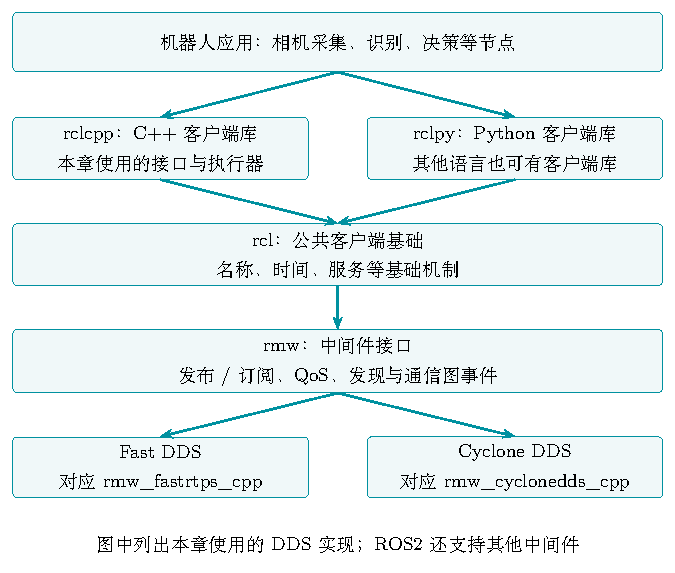
\includegraphics[width=0.8\textwidth]{ros2_arch_revised.pdf}
    \caption{本章使用的 ROS2 软件分层}
    \label{fig:ros2_arch}
\end{figure}
常见术语的含义：
\begin{itemize}
    \item \textbf{rclcpp}: ROS Client Library for C++，它是ROS2的C++客户端库，负责ROS2节点的创建、通信、生命周期管理等，我们使用的主要是这个库。
    \item \textbf{rmw}: ROS Middleware，它是ROS2的中间件接口，把上层的通信操作交给具体的中间件实现。
    \item \textbf{QoS}: Quality of Service，它是通信策略的集合，包含历史深度、可靠性、持久性等。
    \item \textbf{DDS}: Data Distribution Service，它是一种发布/订阅通信标准，Fast DDS 与 Cyclone DDS 是它的实现。ROS2 也可以通过 rmw 使用 Zenoh 等其他中间件。
\end{itemize}
\paragraph*{ROS2的节点与组件}
\textbf{ROS2的基本思想是分布式的、模块化的。}

节点（Node）是组织功能的逻辑单元。组件（Component）是可动态装载的节点实现，组件容器可在同一进程内装载多个节点。
先把下面的节点收发跑通；当图像变大、复制与调度开始影响延迟时，再按第\ref{sec:ros2-image-components}节把相邻节点组合起来。

我们可以用这个图来直观地理解ROS2的\textbf{节点}：
\begin{figure}[htbp]
    \centering
    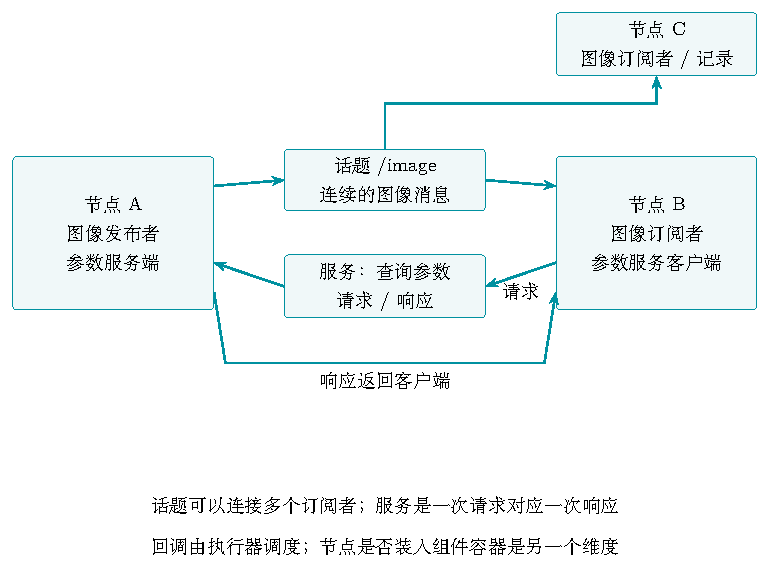
\includegraphics[width=0.8\textwidth]{ros2_node_revised.pdf}
    \caption{节点通过话题与服务通信}
    \label{fig:ros2_node}
\end{figure}

\begin{note}
如果想看节点与话题的动态关系，可以跟着官方节点教程操作：\url{https://docs.ros.org/en/humble/Tutorials/Beginner-CLI-Tools/Understanding-ROS2-Nodes/Understanding-ROS2-Nodes.html}。
\end{note}


这个图直观的反映了ROS2的模块化是依靠\textbf{节点}完成的，节点的职责可以是接收某个传感器的信息（比如相机），也可以是对数据进行处理的流程（比如对相机的图像进行滤波），也可以是提供服务（比如反馈相机的参数信息）
这些功能也可以在一个节点中完成。节点之间通过话题、服务或动作通信；回调由执行器（Executor）调度。


对于我们实际上手操作的情况下，我们更感知的操作方式有两种。
一是使用CLI tools（command-line interface），二是使用Client Libraries。
我们一般使用CLI tools来创建、运行、调试节点，而Client Libraries则用于编写节点的逻辑。

\Needspace{12\baselineskip}
\begin{example}
在终端一加载当前发行版环境后启动 talker；终端二加载相同环境，查询节点与话题：
\par\medskip\noindent\begin{minipage}{\linewidth}
\begin{tbash}
# 终端一
ros2 run demo_nodes_cpp talker
# 终端二
ros2 node list
ros2 topic info /chatter
ros2 topic echo /chatter
\end{tbash}
\end{minipage}\par\smallskip
\end{example}

\begin{exercise}
\label{ex:v2-ros-graph}
记录 /chatter 的消息类型、发布者数量。停止 talker 后重新查询，说明节点与话题的关系。
\end{exercise}

\begin{conclusion}
\begin{itemize}
\item 包组织源码和依赖，节点承担运行时功能，话题传递同类型消息。
\item 组件把节点装入进程；执行器调度回调。
\item QoS 决定通信策略，双方兼容才可能建立连接。
\end{itemize}
\end{conclusion}

\section{工作空间、节点与消息接口}
\subsubsection{创建工作空间与第一个功能包}
由图\ref{fig:ros2_arch}可以看到，rclcpp是ROS2的C++接口，我们在C++中使用这个来描述机器人的节点和节点之间的行为。
首先，你需要寻找一个你喜欢的地方新建一个文件夹，这个名字不重要，但建议起个有意义的名字。
\par\medskip\noindent\begin{minipage}{\linewidth}
\begin{tbash}
    mkdir -p ~/ros2_ws/src
    cd ~/ros2_ws/src
\end{tbash}
\end{minipage}\par\smallskip

这里把工作空间（就是文件夹）命名为ros2\_ws，并在其下创建了一个src文件夹，这个文件夹是ROS2的源代码存放的地方。

接着创建功能包（Package）。包组织代码和依赖，一个包可以包含多个节点程序。
\par\medskip\noindent\begin{minipage}{\linewidth}
\begin{tbash}
    ros2 pkg create --build-type ament_cmake my_package
\end{tbash}
\end{minipage}\par\smallskip
\Needspace{12\baselineskip}
此时的目录结构应类似：
\par\medskip\noindent\begin{minipage}{\linewidth}
\begin{tbash}
ros2_ws/
+-- src/
    +-- my_package/
        +-- CMakeLists.txt
        +-- package.xml
        +-- src/
\end{tbash}
\end{minipage}\par\smallskip

然后回到工作空间的根目录(ros2\_ws),输入以下命令编译这个包：

\par\medskip\noindent\begin{minipage}{\linewidth}
\begin{tbash}
    colcon build
\end{tbash}
\end{minipage}\par\smallskip

编译好的包会产生,build、install、log三个文件夹，其中 build 保存构建中间文件，install 保存安装后的程序、库和环境脚本，log 保存构建日志。

此时的目录结构应类似：
\par\medskip\noindent\begin{minipage}{\linewidth}
\begin{tbash}
ros2_ws/
+-- src/
|   +-- my_package/
|       +-- CMakeLists.txt
|       +-- package.xml
|       +-- src/
+-- build/
+-- install/
+-- log/
\end{tbash}
\end{minipage}\par\smallskip

稍后的完整工程给出普通 ament\_cmake 配置（代码\ref{lst:ros2-basic-cmake}），先学会显式声明依赖与安装目标。

之后我们就可以开始编写代码了。
\subsubsection{用 rclcpp 编写发布者与订阅者}

新建my\_node.cpp和my\_node.h文件。并在这两个文件中新建一个类my\_node，继承自rclcpp::Node。
Node类是ROS2提供的基础的类，我们会在这个基类上进行扩展。

其构造函数一般是用来设置节点的发布者和订阅者，绑定对应的回调函数。实现为代码\ref{lst:my_node_cpp}中的构造函数。
\paragraph*{编写发布者和订阅者}
要编写发布者和订阅者，我们需要使用rclcpp::Publisher和rclcpp::Subscription。
先在节点的类中定义一个私有成员变量，用来保存订阅者的句柄，并在构造函数中初始化。
需要注意，定义的应该是\texttt{rclcpp::Publisher<T>::SharedPtr} 与 \texttt{rclcpp::Subscription<T>::SharedPtr}即共享指针，

初始化的时候需要使用\texttt{create\_publisher<T>} 与 \texttt{create\_subscription<T>}这些模板函数。模板参数是消息类型，两者都要指定话题名和 QoS；订阅者还要提供收到消息后执行的回调。


\par\medskip\noindent\begin{minipage}{\linewidth}
\begin{tcode}
    string_publisher_ = create_publisher<std_msgs::msg::String>(
         "send",
         10
         );
\end{tcode}
\end{minipage}\par\smallskip
这个代码将类的成员变量string\_publisher\_绑定到话题名称为"send"的发布者，历史队列深度为10。这个话题名称是我随便起的，
QoS（Quality of Service，服务质量）包含历史深度、可靠性和持久性等策略。
整数 10 是 KeepLast 历史深度，不是“质量等级”。图像话题常使用 SensorDataQoS；发布与订阅策略必须兼容。
\begin{note}
把队列调大不会让处理更快。图像处理跟不上时，可能只是在积压更旧的帧。
\end{note}
这样变量string\_publisher\_所指的空间就有了一个发布者，它会发布std\_msgs::msg::String类型的消息。但是很明显你能发现它并不会发布消息，因为还没有编写发布消息的逻辑。
不妨在订阅回调中进行发布。

\par\medskip\noindent\begin{minipage}{\linewidth}
\begin{tcode}
    string_subscription_ = create_subscription<std_msgs::msg::String>(
         "receive",
         10,
         std::bind(&my_node::subscription_callback, this, std::placeholders::_1)
         );
\end{tcode}
\end{minipage}\par\smallskip
这个代码将类的成员变量string\_subscription\_绑定到话题名称为"receive"的订阅者，历史队列深度为10。
std::bind 将成员函数与当前对象 this 绑定，占位符 \texttt{std::placeholders::\_1} 接收传入的消息。
也可使用签名匹配的 lambda：\texttt{[this](std\_msgs::msg::String::SharedPtr msg)}。
这个绑定的成员函数就是所谓的订阅回调函数，它会在收到消息时被调用。然后就可以在这个函数中写收到信息之后要干什么了。
\par\medskip\noindent\begin{minipage}{\linewidth}
\begin{tcode}
void my_node::subscription_callback(const std_msgs::msg::String::SharedPtr msg)
{
 RCLCPP_INFO(get_logger(), "I hear %s", msg->data.c_str());
 auto message = std_msgs::msg::String();
 message.data = "I can hear:" + msg->data;
 string_publisher_->publish(message);
}
\end{tcode}
\end{minipage}\par\smallskip

函数体中第一行通过 RCLCPP 的日志系统打印收到的消息。这里使用 INFO 记录正常收包事件；日志级别、输出位置和高频日志限流统一见第\ref{sec:ros2-logging}节。

之后的三行是创建一个String消息类型，并设置它的data字段为收到的消息加上一段文字。然后使用刚刚定义的发布者发布这个消息。

这样我们就完成了一个最简单的ROS2节点，它可以发布和订阅消息，并且可以处理收到的消息。
接下来我们要确认消息真的经过了回调。你可以用 IDE 调试，不过先用终端跑通一遍，更容易判断是程序的问题还是 IDE 环境的问题。完整文件和运行步骤就在后面的第\ref{sec:ros2-project}节。
正式一点来说（比如在实车测试的时候），我们需要在终端中工作空间下，输入以下命令：
\par\medskip\noindent\begin{minipage}{\linewidth}
\begin{tbash}
    colcon build
    source install/setup.bash
    ros2 run my_package my_node
\end{tbash}
\end{minipage}\par\smallskip
然后打开 rqt 的 Message Publisher 与 Message Monitor，分别向话题发布与订阅消息，查看节点运行情况。完整工程跑通后，第\ref{sec:ros2-visualization}节会带我们继续用 rqt、RViz2 和 Foxglove 看曲线、图像与三维图形。

\begin{example}[能看见话题，为什么还收不到消息？]
先暂时放下自己的节点，开两个加载了相同环境的终端，用 CLI 把这个现象单独复现。终端一每秒发送一条消息，明确选择 best\_effort；终端二先要求 reliable：
\par\medskip\noindent\begin{minipage}{\linewidth}
\begin{tbash}
# 终端一
ros2 topic pub /qos_demo std_msgs/msg/String "{data: hello}" --rate 1 --wait-matching-subscriptions 0 --qos-reliability best_effort
# 终端二
ros2 topic echo /qos_demo std_msgs/msg/String --qos-reliability reliable
\end{tbash}
\end{minipage}\par\smallskip
这里把等待订阅者的数量设为 0，让发布端持续发送。你会看见 QoS 不兼容的提示，echo 收不到消息。这时别以为是ROS坏了，急着重装 ROS：只是因为发布端没有提供订阅端要求的可靠性。按 Ctrl+C 停止 echo，再把它的要求改为 best\_effort：
\par\medskip\noindent\begin{minipage}{\linewidth}
\begin{tbash}
ros2 topic echo /qos_demo std_msgs/msg/String --qos-reliability best_effort --once
ros2 topic info /qos_demo --verbose
\end{tbash}
\end{minipage}\par\smallskip
这次应收到 hello；详细信息还能看到各个端点的策略。可靠性只是其中一项，其他策略也必须兼容。结束后停止发布进程，避免它影响后面的实验。
\end{example}
\begin{exercise}
\label{ex:v2-ros-qos}
把发布者改为 reliable、订阅者保留 best\_effort，预测能否收包并实际验证；说明为什么双方策略不必完全相同。
\end{exercise}
\begin{note}
QoS 策略与兼容性表见官方文档：\url{https://docs.ros.org/en/humble/Concepts/Intermediate/About-Quality-of-Service-Settings.html}。
\end{note}

\subsubsection{用定时器周期发布消息}
\begin{note}
日志中的时间用于排查事件顺序。Unix 时间以 UTC 1970 年 1 月 1 日为纪元；ROS 时间还可能由仿真时钟提供，跨节点比较前先确认时钟来源。
\end{note}
这个非常简单，定义rclcpp::TimerBase 类型，然后用C++中的 \texttt{chrono} 库来提供定时器时间，再使用\texttt{create\_wall\_timer}绑定一个函数作为回调函数即可。
\par\medskip\noindent\begin{minipage}{\linewidth}
\begin{tcode}
    //定义成员变量
    rclcpp::TimerBase::SharedPtr timer_;
    //构造函数
    timer_ = create_wall_timer(
        std::chrono::milliseconds(1000), // 定时器间隔
        std::bind(&my_node::timer_callback, this)); // 回调函数
    //回调函数
    void my_node::timer_callback()
    {
        RCLCPP_INFO(get_logger(), "timer count=%d", ++cnt_);
        auto time_msg = std_msgs::msg::String();
        time_msg.data = "Now is " + std::to_string(cnt_);
        timer_publisher_->publish(time_msg);
    }
\end{tcode}
\end{minipage}\par\smallskip
这个回调函数会每秒钟被调用一次，打印一下回调计数，并发布计数消息。

\subsubsection{定义、生成与使用自定义消息}
自定义消息由字段组成。字段可使用基本类型，也可使用 ROS2 已有的消息类型，例如 \path{std_msgs/Header}。
以实际应用例子，我们的机器人在自瞄时传输瞄准的装甲板数据时，需要知道id(敌方装甲板的编号)，yaw(装甲板的偏航角度)等信息。
同时我们还要知道识别到的时间信息。与其把它们塞进一个难以检查的字符串，不如定义一条带类型的消息，让收发两边对字段和单位有共同约定。


在ROS 2中，使用RCLCPP接口创建自定义消息类型需要以下步骤：

1. 创建自定义消息包

首先，创建一个专门用于存放自定义消息的包。例如，创建一个名为my\_msgs的包：
\par\medskip\noindent\begin{minipage}{\linewidth}
\begin{tbash}
    ros2 pkg create --build-type ament_cmake my_msgs
\end{tbash}
\end{minipage}\par\smallskip

然后在该包中创建msg目录，用于存放自定义消息文件。


\begin{note}
包名如 \texttt{my\_msgs} 使用小写字母、数字和下划线，并以字母开头。消息文件名如 \texttt{My.msg} 以大写字母开头，只含字母和数字。两种名字不要混淆。
\end{note}


2. 定义自定义消息

在 msg 目录中创建 My.msg 文件，定义消息结构；yaw 在本例中以弧度表示。
\par\medskip\noindent\begin{minipage}{\linewidth}
\begin{tbash}
    std_msgs/Header header
    uint8 id
    float64 yaw
    bool detect_success
\end{tbash}
\end{minipage}\par\smallskip

3. 修改CMakeLists.txt文件和package.xml文件

建议直接看完整工程的代码\ref{lst:xml_2}

4. 编译自定义消息

在工作空间中运行以下命令以编译自定义消息：
\par\medskip\noindent\begin{minipage}{\linewidth}
\begin{tbash}
    colcon build --packages-select my_msgs
    source install/setup.bash
\end{tbash}
\end{minipage}\par\smallskip

编译后以 \texttt{\#include <my\_msgs/msg/my.hpp>} 引用生成的头文件。

5. 在节点中使用自定义消息

在其他节点中使用自定义消息时，需要在CMakeLists.txt中添加对my\_msgs的依赖，并在代码中包含自定义消息的头文件。就像其他ROS2自带的消息类型一样。


\begin{example}
完成完整工程的消息包后，加载工作空间环境，检查定义是否生成：
\par\medskip\noindent\begin{minipage}{\linewidth}
\begin{tbash}
source ~/ros2_ws/install/setup.bash
ros2 interface show my_msgs/msg/My
\end{tbash}
\end{minipage}\par\smallskip
输出应包含 header、id、yaw、detect\_success 四个字段；Header 的内部字段会展开显示。
\end{example}

\begin{exercise}
\label{ex:v2-ros-message}
给消息加入 float64 distance 字段，重新构建消息包，检查接口输出。约定 distance 单位为米。
\end{exercise}
\subsubsection{常用消息类型与接口查询}

1.\ std\_msgs

常用消息包括 \texttt{String}、\texttt{Int32}、\texttt{Float64} 等标量与数组类型。
\texttt{std\_msgs/Header} 含 \texttt{stamp}（时间戳）与 \texttt{frame\_id}（坐标系标识），几何与传感器消息常内嵌该头。

除了 std\_msgs，常用消息集合 common\_msgs 中还有 \texttt{geometry\_msgs}、\texttt{nav\_msgs}、\texttt{sensor\_msgs} 等。

2.geometry\_msgs。最常用的几何消息类型，定义了描述机器人状态的各种类型，比如点、速度、加速度、位姿等。

Vector3 用三个 float64 描述三维向量，例如速度或方向；表示空间中的位置点通常用 Point。两者看起来都有 x、y、z，不过表示的实际物理含义不同。带 Stamped 后缀的类型还提供 Header，让我们知道数据来自哪个坐标系、对应哪个时刻。
Quaternion、QuaternionStamped是传输四元数的消息类型。
Transform、TransformStamped是传输坐标系变换关系的消息类型。

3.sensor\_msgs。包含了传感器数据，包括图像、激光、雷达、IMU等。

主要用的就上面三种消息类型。



更多更详细内容请参考官方文档。

\begin{example}
完成本章完整工程后，查看接口定义并只接收一次定时器消息：
\par\medskip\noindent\begin{minipage}{\linewidth}
\begin{tbash}
source /opt/ros/humble/setup.bash
source ~/ros2_ws/install/setup.bash
ros2 interface show my_msgs/msg/My
ros2 interface show geometry_msgs/msg/Vector3
ros2 interface show geometry_msgs/msg/Point
ros2 interface show sensor_msgs/msg/Image
ros2 topic echo /timer_ --once
\end{tbash}
\end{minipage}\par\smallskip
先对照 Vector3 与 Point 的注释，再看看 Image 除了像素数据还有哪些描述字段。Header 的 frame\_id 只是坐标系标识，写一个名字不会替你完成坐标变换：后面使用 tf2 时才会把坐标系之间的关系连起来。
\begin{note}
Image 包含 height、width、encoding、step 和 data 等字段，CompressedImage 则描述压缩格式和压缩后的数据，别把它们混在一起。需要核对原始定义时，可以直接查看包中的消息文件：
\par\medskip\noindent\begin{minipage}{\linewidth}
\begin{tbash}
cat "$(ros2 pkg prefix --share sensor_msgs)/msg/Image.msg"
\end{tbash}
\end{minipage}\par\smallskip
这里查看的是 \texttt{sensor\_msgs::msg::Image} 的消息定义；它与\texttt{CompressedImage}是两个不同的类型。
\end{note}
\end{example}

\begin{exercise}
\label{ex:v2-ros-timer}
将定时器间隔改为 500 ms，重编译并用 ros2 topic hz /timer\_ 检查频率；再解释消息中的时间戳与计数器有何不同。
\end{exercise}

\begin{conclusion}
\begin{itemize}
\item 编辑 src 中的文件，回到工作空间根目录编译。
\item build 是构建过程，install 是运行入口，使用前加载 setup.bash。
\item 自定义接口先声明字段与依赖，再生成代码；订阅、发布和定时器句柄要持续存活。
\end{itemize}
\end{conclusion}

\subsubsection{服务调用与后续工具}
这部分是一些ROS2的较高级内容，主要是介绍名字和基本用途。
可以在需要的时候查找对应关键词。

\textbf{功能:}
\begin{enumerate}
    \item ROS2 launch，可以用来启动多个节点，并设置参数。用于启动复杂的系统。
    \item service的代码实现
    \item ROS2参数，可以通过launch文件设置参数，也可以在代码中设置参数。
    \item rosbag 用于记录和重放ROS2的消息。这点对于调试和分析非常有用，可以做到在家就能调试。
    \item 通过ROS2组件的形式启动ROS2节点。
\end{enumerate}

\textbf{包:}
\begin{enumerate}
    \item cv\_bridge 包，用于ROS2和OpenCV之间的互相转换。
    \item camera\_calibration 用于相机标定，配合参数管理与 image\_proc 图像校正；完整流程见第\ref{sec:ros2-camera-calibration}节。
    \item tf2 包，提供了一个坐标变换的框架。
    \item RViz2 用于可视化坐标系、位姿、轨迹和图形消息；rqt 与 Foxglove 的曲线、图像、标注和回放也会在第\ref{sec:ros2-visualization}节练习。
    \item moveit2 包，用于机械臂控制。
    \item navigation2 包，用于导航。
\end{enumerate}

\begin{example}
使用已安装的 demo 服务。终端一运行服务端，终端二调用后应得到 sum: 5。
\par\medskip\noindent\begin{minipage}{\linewidth}
\begin{tbash}
# 两个终端都先加载同一发行版环境
# 终端一
ros2 run demo_nodes_cpp add_two_ints_server
# 终端二
ros2 service call /add_two_ints example_interfaces/srv/AddTwoInts "{a: 2, b: 3}"
\end{tbash}
\end{minipage}\par\smallskip
\end{example}

\begin{exercise}
\label{ex:v2-ros-service}
用服务列表和接口查询命令查出该服务的请求、响应字段；说明这种一次请求与持续发布话题的区别。
\end{exercise}


\section{完整工程与收发验证}
\subsubsection{完整工程：组织文件并生成消息接口}
\label{sec:ros2-project}
刚才我们逐段写了节点和消息接口，现在把它们拼成一个能运行的小工程。完整源码就在本卷 \path{examples/ros2/basic-interfaces-demo}，包括两个包。my\_msgs 先生成消息类型，my\_package 再使用它；文件之间的关系如下：
\par\medskip\noindent\begin{minipage}{\linewidth}
\begin{lstlisting}[language={}]
basic-interfaces-demo/
  README.md
  my_msgs/
    CMakeLists.txt
    package.xml
    msg/My.msg
  my_package/
    CMakeLists.txt
    package.xml
    include/my_package/my_node.h
    src/my_node.cpp
    src/node_run.cpp
\end{lstlisting}
\end{minipage}\par\smallskip
你可以照着下面写，也可以把两个包复制到新工作空间的 src 中，再逐个核对。

\begin{example}[准备消息包与接口生成规则]
首先准备消息包。这个文件只写字段，不写 C++ 类定义，构建工具会自动生成代码。
\par\medskip\noindent\begin{minipage}{\linewidth}
\lstinputlisting[frame=single,language={},caption={my\_msgs/msg/My.msg}]{examples/ros2/basic-interfaces-demo/my_msgs/msg/My.msg}
\end{minipage}\par\smallskip

下面两份文件让 ROS2 知道“要生成哪个接口、依赖哪些类型”。std\_msgs 提供 Header，rosidl 提供接口代码生成过程；这两项都要先安装好。
\par\medskip\noindent\begin{minipage}{\linewidth}
\lstinputlisting[frame=single,language=cmake,label=lst:cmake_2,caption={my\_msgs/CMakeLists.txt}]{examples/ros2/basic-interfaces-demo/my_msgs/CMakeLists.txt}
\end{minipage}\par\smallskip
\par\medskip\noindent\begin{minipage}{\linewidth}
\lstinputlisting[frame=single,language=XML,label=lst:xml_2,caption={my\_msgs/package.xml}]{examples/ros2/basic-interfaces-demo/my_msgs/package.xml}
\end{minipage}\par\smallskip

\end{example}

\Needspace{35\baselineskip}
\subsubsection{完整工程：实现节点并声明构建依赖}
\begin{example}[把发布、订阅和定时器接起来]
接下来准备节点包。头文件声明节点类并保存发布者、订阅者和定时器句柄；把句柄放在成员中，节点运行时它们才会一直存活。
\par\medskip\noindent\begin{minipage}{\linewidth}
\lstinputlisting[frame=single,language=C++,label=lst:my_node_h,caption={my\_package/include/my\_package/my\_node.h},numbers=left,numberstyle={\color{gray}\tiny}]{examples/ros2/basic-interfaces-demo/my_package/include/my_package/my_node.h}
\end{minipage}\par\smallskip

实现文件中的构造函数先创建各个接口并绑定回调。收到 receive 后，字符串回调把内容加上前缀发到 send；定时器每秒发布一次计数和自定义消息。节点还订阅自己的 my\_msg，方便你在日志里看见字段确实经过了通信。
\lstinputlisting[frame=single,language=C++,lastline=52,label=lst:my_node_cpp,caption={my\_package/src/my\_node.cpp},numbers=left,numberstyle={\color{gray}\tiny}]{examples/ros2/basic-interfaces-demo/my_package/src/my_node.cpp}
定时器回调再填入时间戳、坐标系和检测结果，然后发布消息。下面接着展示同一文件，行号保持连续：
\par\medskip\noindent\begin{minipage}{\linewidth}
\lstinputlisting[frame=single,language=C++,firstline=53,firstnumber=53,lastline=68,caption={my\_node.cpp 的定时器回调},numbers=left,numberstyle={\color{gray}\tiny}]{examples/ros2/basic-interfaces-demo/my_package/src/my_node.cpp}
\end{minipage}\par\smallskip

\Needspace{9\baselineskip}
文件最后的自订阅回调只负责打印字段。这样我们不用再写第二个节点，也能先检查自定义消息是否按约定传了过来：
\par\medskip\noindent\begin{minipage}{\linewidth}
\lstinputlisting[frame=single,language=C++,firstline=69,firstnumber=69,caption={my\_node.cpp 的自定义消息回调},numbers=left,numberstyle={\color{gray}\tiny}]{examples/ros2/basic-interfaces-demo/my_package/src/my_node.cpp}
\end{minipage}\par\smallskip


最后由入口文件初始化 ROS2、创建节点并调用 spin。spin 让执行器调度回调。如果只创建对象却不进入执行器，回调不会按上面的预期工作。
\par\medskip\noindent\begin{minipage}{\linewidth}
\lstinputlisting[frame=single,language=C++,label=lst:node_run_cpp,caption={my\_package/src/node\_run.cpp},numbers=left,numberstyle={\color{gray}\tiny}]{examples/ros2/basic-interfaces-demo/my_package/src/node_run.cpp}
\end{minipage}\par\smallskip

节点包的构建规则显式找到 rclcpp、std\_msgs 和刚才的 my\_msgs，创建 my\_node 目标，并把它安装到 ROS2 能查到的位置。包清单中的 my\_msgs 依赖也让 colcon 能按正确顺序构建两个包。
\par\medskip\noindent\begin{minipage}{\linewidth}
\lstinputlisting[frame=single,language=cmake,label=lst:ros2-basic-cmake,caption={my\_package/CMakeLists.txt}]{examples/ros2/basic-interfaces-demo/my_package/CMakeLists.txt}
\end{minipage}\par\smallskip
\Needspace{19\baselineskip}
\par\medskip\noindent\begin{minipage}{\linewidth}
\lstinputlisting[frame=single,language=XML,label=lst:xml_1,caption={my\_package/package.xml}]{examples/ros2/basic-interfaces-demo/my_package/package.xml}
\end{minipage}\par\smallskip

\end{example}

\subsubsection{完整工程：编译并验证话题收发}
\begin{example}[先生成接口，再启动节点]
把两个包放进 \path{~/ros2_ws/src} 后，回到工作空间根目录构建。
\par\medskip\noindent\begin{minipage}{\linewidth}
\begin{tbash}
source /opt/ros/humble/setup.bash
cd ~/ros2_ws
colcon build --packages-up-to my_package
source install/setup.bash
ros2 run my_package my_node
\end{tbash}
\end{minipage}\par\smallskip
\texttt{--packages-up-to} 同时构建工作空间中的消息依赖。节点应每秒记录一次 timer count，并打印 id 为 1、yaw 为 0.25 的自定义消息。

终端二加载同一系统与工作空间环境后观察一次消息：
\par\medskip\noindent\begin{minipage}{\linewidth}
\begin{tbash}
source /opt/ros/humble/setup.bash
source ~/ros2_ws/install/setup.bash
ros2 topic echo /my_msg --once
ros2 topic echo /timer_ --once
ros2 topic echo /send
\end{tbash}
\end{minipage}\par\smallskip
先保持 send 的观察进程运行，再开一个同样加载环境的终端发送：
\par\medskip\noindent\begin{minipage}{\linewidth}
\begin{tbash}
ros2 topic pub --once /receive std_msgs/msg/String "{data: hello}"
\end{tbash}
\end{minipage}\par\smallskip
节点日志应显示收到 hello，send 应收到 I can hear:hello。按 Ctrl+C 结束节点和观察进程，再修改代码做练习。
\end{example}

\subsubsection{用 rqt 发布输入与监视回复}
\begin{example}[用 rqt 看见同一条消息经过了哪里]
终端里的收发已经跑通了，我们再把它搬到图形界面。先让 my\_node 保持运行，在同样加载了环境的两个终端分别打开插件：
\par\medskip\noindent\begin{minipage}{\linewidth}
\begin{tbash}
ros2 run rqt_gui rqt_gui --standalone rqt_publisher
ros2 run rqt_gui rqt_gui --standalone rqt_topic
\end{tbash}
\end{minipage}\par\smallskip
如果缺少插件，用 \texttt{sudo apt install ros-humble-rqt-publisher ros-humble-rqt-topic} 安装。

在 Message Publisher 中选择话题 /receive、类型 \texttt{std\_msgs/msg/String}，添加发布者。展开 data 字段，在 expression 列填入带引号的 Python 字符串 \texttt{'armor\_found'}，再勾选发布者启用发送。在 Message Monitor 中勾选 /receive、/send、/my\_msg 与 /timer\_ 并展开字段；你应看到输入、带前缀的回复和持续变化的计数，yaw 则保持 0.25。若没有值，先确认勾选的是话题左侧的监视框，再检查环境和消息类型。

\begin{figure}[htbp]
  \centering
  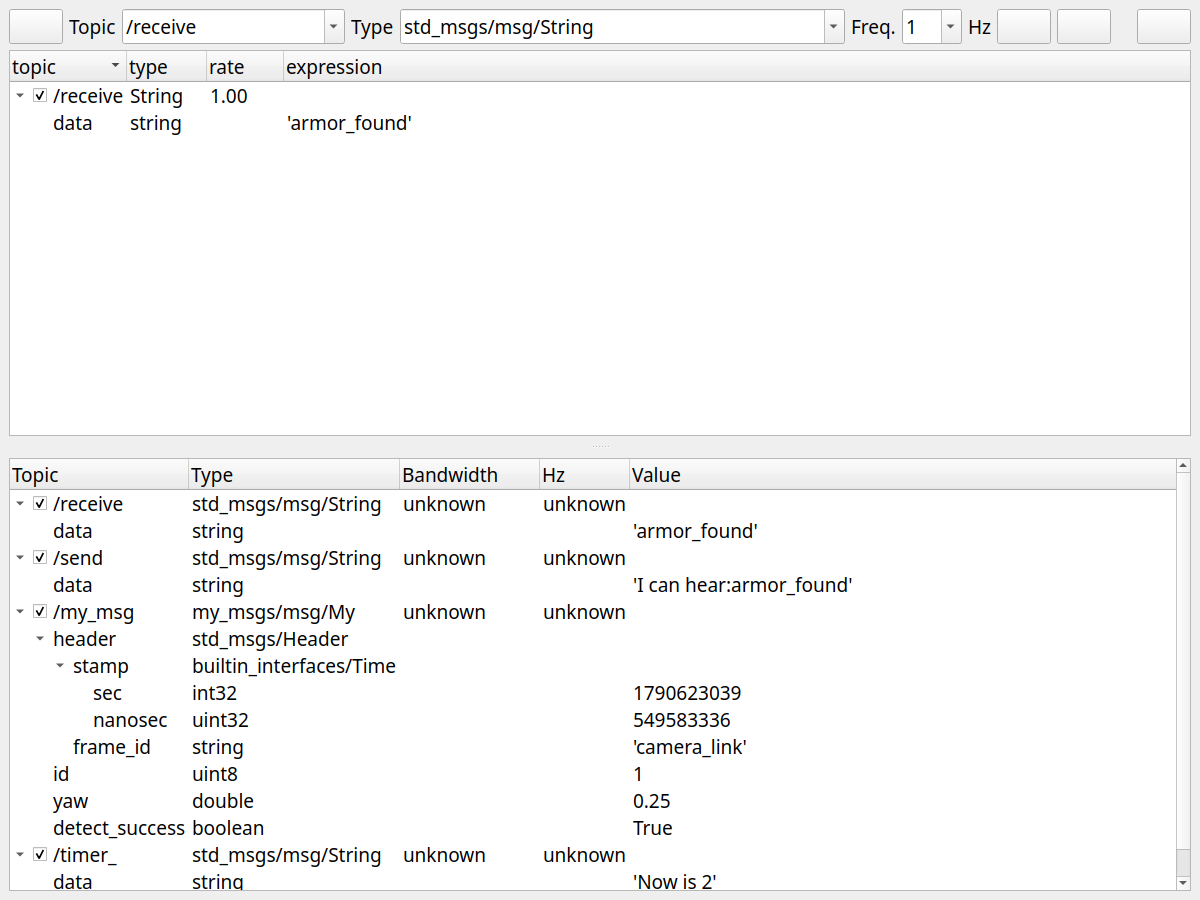
\includegraphics[width=0.8\textwidth]{ros2_rqt_revised.png}
  \caption{rqt 发布与监视插件：对照 receive 的输入与 send 的回复}
  \label{fig:ros2-rqt}
\end{figure}

图\ref{fig:ros2-rqt}中，上半部分是发布输入，下半部分是监视结果。重点看两条 data：输入是 armor\_found，回复多了 I can hear:，这正是字符串回调做的事情。你的窗口摆放可以不同，字段与话题应对应得上。

现在按 Ctrl+C 停止 my\_node。发布端还能发送 receive，但 send 不再有新回复；监视器可能暂时保留最后一条数据。重新启动节点后，如果话题条目被移除了，就重新勾选监视，再确认回复恢复。
\end{example}

\begin{exercise}
\label{ex:v2-ros-reply}
保持完整工程中的节点运行，把输入 hello 换成 armor\_found；记录 receive、send 的消息类型与返回内容。停止节点后再发一次，说明“命令发出了消息”和“程序处理了消息”有什么区别。
\end{exercise}

\section{rqt 与 RViz2 图形化观测}
\subsubsection{把消息画出来：先准备一组能对照的数据}
\label{sec:ros2-visualization}

前面我们已经在终端和 rqt 的消息监视器里看见了字段。不过，坐标在不在抖、图像有没有变色、检测框是不是跟着目标走，盯着一屏数字就有些费眼睛了。接下来我们把同一组数据放到曲线、图像和三维窗口里看。以后调程序时，你就可以把“好像不对”变成更具体的判断：哪一条曲线变了，哪一个坐标系反了，或者哪一帧的标注没有对上。

rqt 是一组可以拼在同一窗口里的 ROS 插件，适合快速发布、查字段、画曲线和看图像；RViz2 擅长把 ROS 的坐标系、位姿、轨迹和图形消息放进三维场景；Foxglove 则把这些观测放到一个布局里，还能通过桥接连接机器人、回放录制文件，并在曲线上做换算和测量。我们先把数据源准备好，再分别打开它们。

\begin{example}[一份数据源，三种观察方式]
本卷的 \path{examples/ros2/visualization-demo} 不需要相机，直接生成一块左右移动的绿色色块，以及绕圆运动的目标。它每 0.1 秒发布一次，话题与用途如下。
\begin{center}
\begin{tabular}{p{0.23\linewidth}p{0.38\linewidth}p{0.31\linewidth}}
\toprule
话题 & 消息类型 & 用来看什么\\
\midrule
\path{/viz/signal} & \path{std_msgs/msg/}\newline\path{Float64} & 正弦曲线\\
\path{/viz/pose} & \path{geometry_msgs/msg/}\newline\path{PoseStamped} & 位置与四元数朝向\\
\path{/viz/twist} & \path{geometry_msgs/msg/}\newline\path{TwistStamped} & 速度向量与角速度\\
\path{/viz/path} & \path{nav_msgs/msg/}\newline\path{Path} & 最近 120 个位置\\
\path{/viz/image} & \path{sensor_msgs/msg/}\newline\path{Image} & 640×360 的 rgb8 原图\\
\path{/viz/markers} & \path{visualization_msgs/msg/}\newline\path{MarkerArray} & 球、箭头、轨迹与文字\\
\path{/viz/annotations} & \path{foxglove_msgs/msg/}\newline\path{ImageAnnotations} & 二维框、中心点与标签\\
\path{/viz/scene} & \path{foxglove_msgs/msg/}\newline\path{SceneUpdate} & Foxglove 原生三维实体\\
\path{/tf} & \path{tf2_msgs/msg/}\newline\path{TFMessage} & map 到 target 的坐标变换\\
\bottomrule
\end{tabular}
\end{center}

先在 Ubuntu 22.04 / Humble 环境中安装本节用到的工具。之前装了 desktop 的话，RViz2 和部分 rqt 插件可能已经有了，再执行安装会由 apt 检查。
\par\medskip\noindent\begin{minipage}{\linewidth}
\begin{tbash}
source /opt/ros/humble/setup.bash
sudo apt update
sudo apt install ros-humble-rqt ros-humble-rqt-graph \
  ros-humble-rqt-publisher ros-humble-rqt-topic \
  ros-humble-rqt-plot ros-humble-rqt-image-view \
  ros-humble-rviz2 ros-humble-foxglove-msgs \
  ros-humble-tf2-ros python3-pyqtgraph
cd /你的教材目录/02-专项技术栈/examples/ros2/visualization-demo
python3 data_node.py
\end{tbash}
\end{minipage}\par\smallskip
把 cd 后的路径换成你的实际目录；几个 Python 文件放在同一目录，直接运行即可，不需要再创建功能包。后面开出的终端都加载同一套 Humble 环境，通信域与发现范围也保持一致。先让这个终端持续运行，在另一终端用 \texttt{ros2 topic list -t} 找到上表的话题，再用 \texttt{ros2 topic echo /viz/pose --once} 确认能收到消息。

项目文件很少，data\_node.py 负责定时发布，另外三个文件分别填写三维 Marker、图像标注和 Foxglove 场景；demo.rviz 保存本节的显示配置。下面先把数据源的完整代码放出来，三种图形消息的代码留到讲它们时再看。
\begin{lstlisting}[language={}]
visualization-demo/
  README.md
  data_node.py
  markers.py
  annotations.py
  scene.py
  demo.rviz
\end{lstlisting}
\lstinputlisting[language=Python,basicstyle=\ttfamily\fontsize{9.5}{11.5}\selectfont,caption={data\_node.py：统一生成位姿、曲线与图像}]{examples/ros2/visualization-demo/data_node.py}

构造函数保存发布者、TF 广播器和定时器，回调每次只取一次时间，供这组消息共用。位置沿着半径 1 m 的圆运动，线速度是位置对时间的导数；ROS使用四元数用来表示朝向，orientation.z 的含义不是 yaw。最近 120 个位姿组成 Path，\texttt{map -> target} 的 TF 则告诉查看器目标坐标系在哪里。

图像部分直接填入 RGB 字节：每个像素三个字节，所以 step 是 $640\times3$，data 的长度是 $360\times\text{step}$。绿色色块已经在原图里，检测框和文字由另一条标注话题提供。这样我们可以分别检查“图像到了没有”和“算法结果对上了没有”。这里只用合成色块演示接口，后面的 OpenCV 章节再把它换成实际图像处理。
\end{example}

\begin{exercise}\label{ex:v2-ros-viz-source}
启动数据源，记录 pose、image 和 annotations 的类型与一组时间戳。根据图像的 width、height、encoding、step 判断 data 应有多少字节；说明为什么标注需要沿用这帧图像的时间，而不是算法算完后的时间。
\end{exercise}

\subsubsection{rqt：连线、曲线与图像都看一遍}
\label{sec:ros2-rqt-views}

刚才的 Message Publisher 与 Message Monitor 解决了“发了什么、收到了什么”。现在再补上三个常用插件。你可以运行 \texttt{rqt}，从 Plugins 菜单依次加入 Introspection 下的 Node Graph、Visualization 下的 Plot 和 Image View；不同版本的菜单排法可能稍有变化，按插件名找即可。插件窗口可以拖动并停靠，常用布局通过 Perspectives 保存，下次打开再恢复。

\begin{example}[把位置变化与图像变化同时看见]
保持数据源运行，在加载环境的终端里按需打开下面的独立窗口，每条启动命令各占一个终端。通用写法是 \texttt{ros2 run <包名> <程序名> [插件参数]}，rqt\_plot 后面接要画的数值字段。
\par\medskip\noindent\begin{minipage}{\linewidth}
\begin{tbash}
ros2 run rqt_graph rqt_graph
ros2 run rqt_plot rqt_plot \
  /viz/signal/data /viz/pose/pose/position/x
ros2 run rqt_image_view rqt_image_view /viz/image
\end{tbash}
\end{minipage}\par\smallskip

在 Node Graph 里点击刷新，选择显示节点与话题的模式，找到 viz\_demo 到各话题的连线。查看器自己也是订阅者，会出现在图中；如果打开了隐藏叶子话题或调试节点的选项，一些线可能被过滤掉。它适合查“谁连接谁”，具体数据仍要到 Monitor、Plot 和 Image View 中看。

Plot 的输入框填 \path{/viz/signal/data}，点加号添加曲线；再填 \path{/viz/pose/pose/position/x} 添加第二条。这里用斜线走到消息内部的数值字段，不能只填整个 Pose。两条曲线分别是 $\sin t$ 与 $\cos t$，幅值约为 1，相差四分之一个周期。点击暂停可以冻结显示，移除曲线用减号或曲线菜单；缩放后用自动缩放或重置视图找回数据。不同绘图库的按钮位置会有差别，切换到 PyQtGraph 后再检查图例和坐标轴。

图\ref{fig:ros2-rqt-plot} 是这份数据在 Humble 的 rqt Plot 插件中实际画出的结果。蓝线看 signal.data，红线看 pose.position.x，先找幅值与相位关系，再回到数值字段核对。截图使用 PyQtGraph，并放大图例字号以便在书页里阅读。
\begin{figure}[htbp]
  \centering
  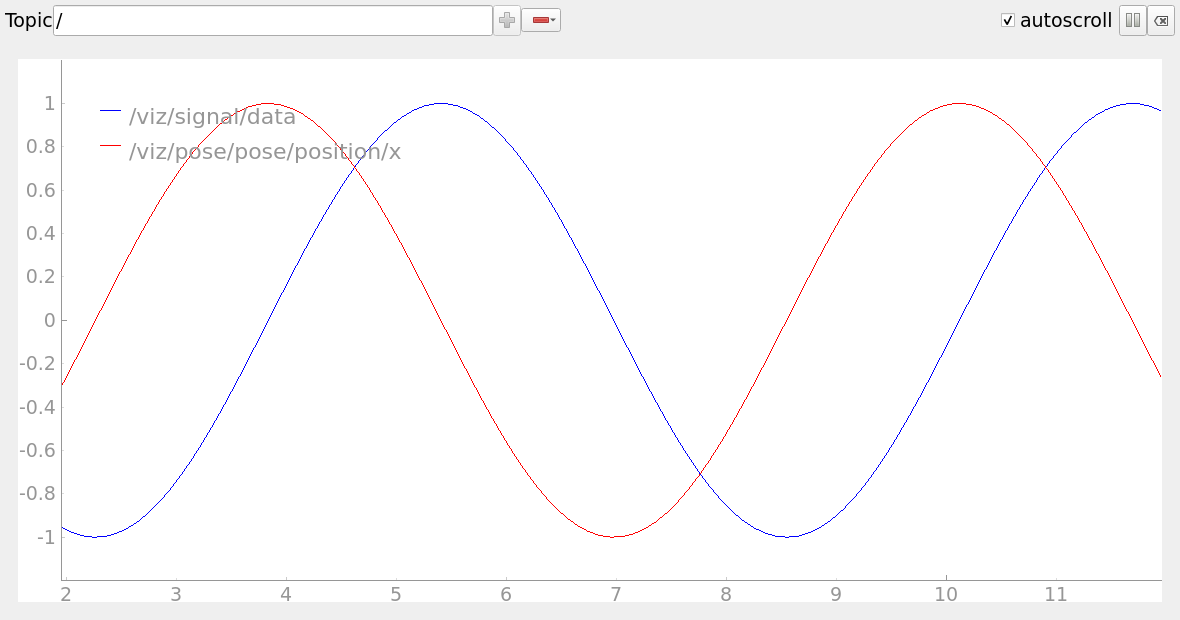
\includegraphics[width=\linewidth]{images/ros2_rqt_plot_revised.png}
  \caption{同一数据源的两条曲线：幅值约为 1，相差四分之一个周期}
  \label{fig:ros2-rqt-plot}
\end{figure}

Image View 的话题下拉框选择 \path{/viz/image}，传输方式使用 raw。你应看到深色背景上的绿色色块来回运动。调整窗口大小或缩放显示时注意保持纵横比，保存图像的按钮可以留下当前画面，后续对照算法结果会用得上。换到实际相机时，若驱动提供 compressed 传输，再选择对应方式；compressedDepth 用于深度图，不能当作普通彩色 JPEG 来选。

曲线空白时，先用 topic echo 确认字段有数据，再检查字段是不是数值、发布端是否仍在运行。图像空白时，检查话题类型和 QoS，并核对 encoding、step 与数据长度；红蓝颠倒往往是 RGB/BGR 顺序写错。rqt\_plot 使用自身的时间轴，不适合单凭两个窗口的横坐标判断传感器采集延迟。需要按消息时间对齐和测量时，我们下面用 Foxglove 再做一次。
\end{example}

\begin{exercise}\label{ex:v2-ros-rqt-views}
把 pose.position.y 加入曲线，与 x 对照，保存一张曲线和一帧原图。停止数据源，观察曲线与图像是否还保留最后结果，再重新启动。说明“窗口还有图”和“现在还在收到数据”有什么区别。
\end{exercise}

\subsubsection{RViz2：让坐标系、轨迹和图形各就各位}
\label{sec:ros2-rviz}

图像里的框只有像素位置，三维目标则还要说明相对于哪个坐标系。RViz2 的 Fixed Frame 是整个场景用来对齐数据的参考坐标系。比如消息写的是 camera，场景选的是 map，查看器就需要同一时刻从 camera 到 map 的 TF。本例的三维消息都写 map，并广播 map 到 target 的变换；图像的 camera\_optical 只用于二维原图显示，没有在这里假装完成相机外参标定。

\begin{example}[先手动加显示，再保存配置]
保持数据源运行，另开终端执行 \texttt{rviz2}。先在左侧 Global Options 中把 Fixed Frame 改成 \texttt{map}，再点 Add，按显示类型逐个添加：
\begin{center}
\begin{tabular}{p{0.20\linewidth}p{0.26\linewidth}p{0.46\linewidth}}
\toprule
显示类型 & 话题 & 观察结果\\
\midrule
Grid、TF & TF 订阅 /tf & 地面网格与 map、target 坐标轴\\
Pose & \path{/viz/pose} & 沿圆运动并转向的位姿箭头\\
Path & \path{/viz/path} & 最近 120 个位置连成的轨迹\\
MarkerArray & \path{/viz/markers} & 球、方向箭头、轨迹和文字\\
Image & \path{/viz/image} & 独立的二维原图窗口\\
\bottomrule
\end{tabular}
\end{center}
本例发布端使用 Reliable、Volatile、深度 10，先让各显示使用匹配的 QoS。接入常用的 Best Effort 相机或点云时，再在该显示的 Topic 属性中把 Reliability 调为 Best Effort。展开显示项的 Status 能看见错误原因；遇到 No transform 时先核对 frame\_id、时间戳和 TF 链，不要只把消息里的坐标系名字改成 map 来消掉提示。

视图选 Orbit，左键拖动旋转观察、滚轮拉近拉远；工具栏的 Move Camera 用于观察，Select 用于选中对象，Focus Camera 可以把视角移到目标附近。熟悉后通过 File / Save Config As 保存自己的 \texttt{.rviz} 文件。项目也提供了相同话题的配置，在项目目录中执行下面的命令即可恢复：
\par\medskip\noindent\begin{minipage}{\linewidth}
\begin{tbash}
rviz2 -d demo.rviz
ros2 run tf2_ros tf2_echo map target
\end{tbash}
\end{minipage}\par\smallskip
两个命令各占一个终端。前者打开显示，后者独立检查坐标变换；持续变化的平移和旋转应与场景中的 target 对应。Pose 是一份位置和朝向，Path 是一串带时间的位姿，TF 则连接坐标系，画面上看着相似的线和箭头，背后的消息各有用途。
图\ref{fig:ros2-rviz-views} 用提供的配置实际打开了这些显示。左上是原图，右边的蓝色球、切线方向箭头、黄色轨迹和 target 文字来自 MarkerArray；红色箭头来自 Pose，坐标轴来自 TF。
\begin{figure}[htbp]
  \centering
  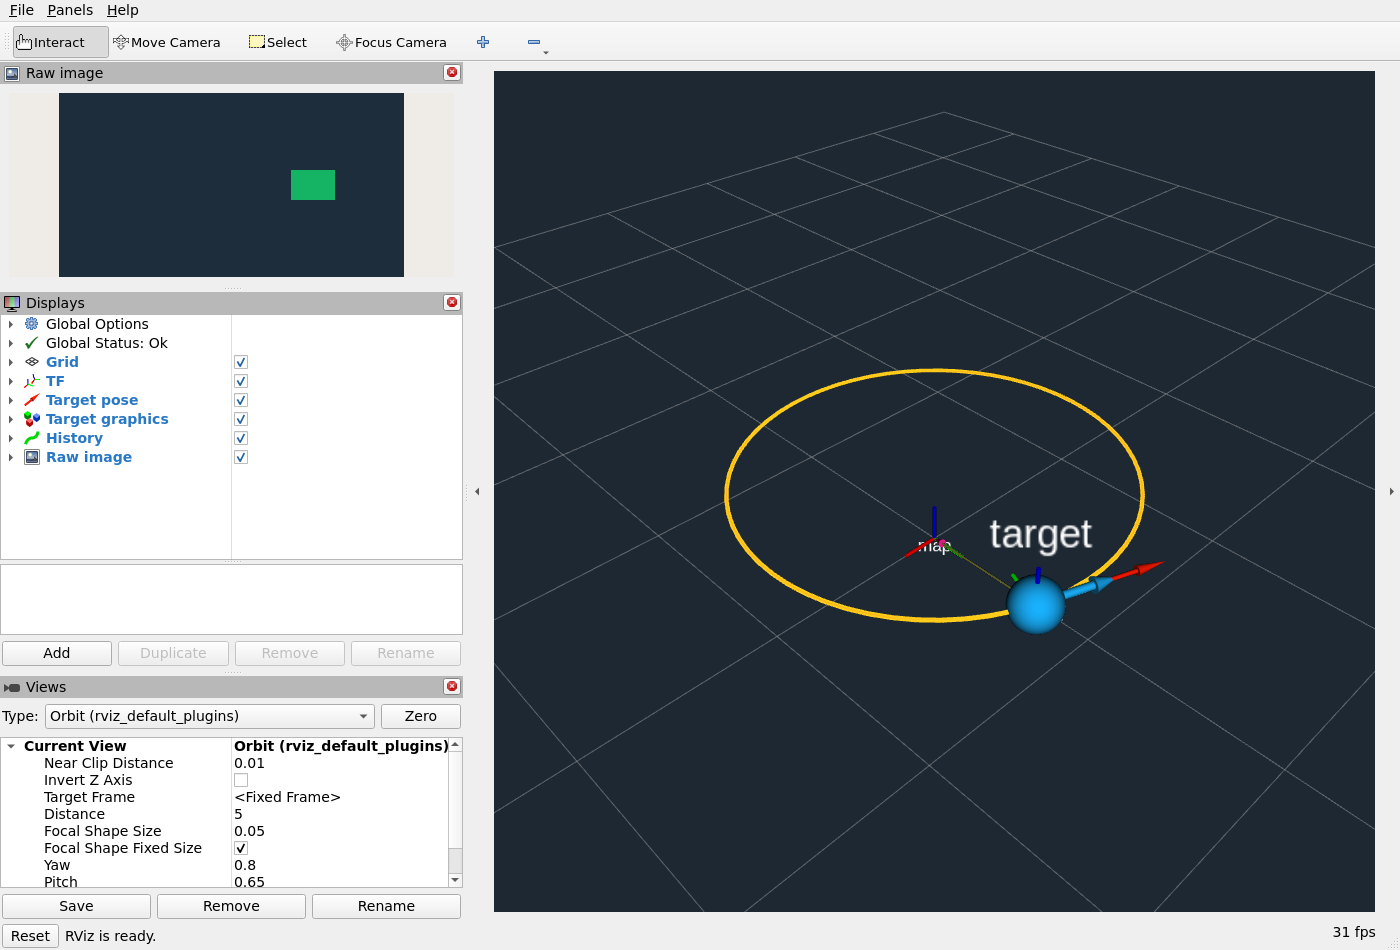
\includegraphics[width=\linewidth]{images/ros2_rviz_views_revised.png}
  \caption{Humble 中实际显示的原图、目标图形、位姿、轨迹与坐标轴}
  \label{fig:ros2-rviz-views}
\end{figure}
\end{example}

\subsubsection{Marker：绘制、更新与删除三维图形}
要给目标画一个球、给速度画一支箭头，或者在旁边放上编号，我们发布 \path{visualization_msgs/msg/Marker}。一次要更新多个图形时，把它们放进 MarkerArray.markers。RViz2 分别使用 Marker、MarkerArray 显示，Foxglove 的 3D 面板也能读取这两种 ROS 消息。

\begin{example}[球、箭头、轨迹和文字共用一份目标位置]
下面就是数据源调用的完整 markers.py。你可以对照每个图形的 type，再回到窗口找它。
\Needspace{8\baselineskip}
\lstinputlisting[language=Python,basicstyle=\ttfamily\fontsize{9.5}{11.5}\selectfont,caption={markers.py：填写并更新四种三维图形}]{examples/ros2/visualization-demo/markers.py}

\texttt{header.frame\_id} 决定坐标属于哪里，stamp 用来查相应时刻的 TF；pose 放图形的位置与朝向，单位四元数 \texttt{w=1} 表示不旋转。\texttt{ns} 和 id 一起标识图形，本例固定用 target 下的 0、1、2、3。下一次收到相同组合的 ADD，会更新已有图形，所以它能跟着目标移动；每帧都换一个新 id，则容易把过去的目标留满屏幕。

球的 scale 三个分量是三个方向的直径，CUBE 对应三个方向的边长；本例球的直径是 0.25 m。箭头可以用 pose 与长度表示，也可以像这里用 points 写出起点和终点；使用两点时，scale.x、y、z 分别控制箭杆直径、箭头直径和箭头长度。LINE\_STRIP 依次连接点，scale.x 是线宽；LINE\_LIST 每两个点画一段独立线，点数要成对。POINTS 用 scale.x、y 控制点的宽高，TEXT\_VIEW\_FACING 则用 scale.z 控制字高，内容填 text。

color 的 r、g、b、a 都在 0 到 1 之间，尤其别忘记 a：默认的 0 会让图形完全透明。给每个点设置 colors 时，数组长度要与 points 对应。需要网格模型还可以用 MESH\_RESOURCE 和 \texttt{package://包名/路径/model.dae} 等资源地址，先确认资源可被查看器读取，再考虑材质设置。更多图形类型可以查\href{https://github.com/ros2/ros2_documentation/blob/humble/source/Tutorials/Intermediate/RViz/Marker-Display-types/Marker-Display-types.rst}{Humble 的 Marker 类型说明}。

lifetime 设为 0 会一直保留，直到被更新或删除；本例设为 0.5 秒，每次更新重新计时，停止发布后就能看到图形消失。DELETE 删除同一个 ns/id，DELETEALL 清理该显示中的图形，通常不要在多人共用的话题上随手发送清空命令。\texttt{frame\_locked=true} 会让图形随着其 frame 的新 TF 移动；默认 false 按收到消息时的变换放置，是否持续跟随要按图形含义选择。

现在在另一终端切换本例的参数，先执行 false 并观察，再执行 true：
\par\medskip\noindent\begin{minipage}{\linewidth}
\begin{tbash}
ros2 param set /viz_demo show_target false
ros2 param set /viz_demo show_target true
\end{tbash}
\end{minipage}\par\smallskip
false 时 id 为 0 的球收到 DELETE，其他箭头、文字与轨迹继续显示；true 时再次 ADD 恢复球。这比只往消息数组里删掉球更明确：数组里没出现一个 id，并不表示查看器要删除它。
\end{example}

\begin{conclusion}
读三维画面时，我们要能回答三个问题：数据属于哪个坐标系，图形的尺寸和颜色有没有填对，同一个对象怎样更新和结束。TF 帮助对齐坐标，Marker 的 ns/id 帮助更新对象，lifetime 与删除动作帮助清理过期结果。它们都需要消息里的约定，查看器不会替我们猜。
\end{conclusion}

\begin{exercise}\label{ex:v2-ros-rviz-markers}
把球改成边长 0.25 m 的立方体，再改变颜色和寿命，记录结果。解释把 alpha 留成 0、每帧改 id、只从 MarkerArray 中移除一个元素各会发生什么；用 show\_target 演示明确删除与恢复。
\end{exercise}

\section{Foxglove：连接、观测与回放}
\subsubsection{Foxglove：安装、连接与保存自己的观察布局}
\label{sec:ros2-foxglove}

接下来我们把刚才分散的几个窗口放在一起。Foxglove 的桌面端与网页端使用相近的面板操作。桌面端安装在你用来观察数据的电脑，foxglove\_bridge 安装在运行 ROS 的环境里；通过桥接传过来的消息定义，如果是跨电脑，桌面端不必再装一整套相同的 ROS 工作空间。

\begin{example}[装好桌面端，再连接自己的数据源]
在 Ubuntu 22.04 中先用 \texttt{dpkg --print-architecture} 看架构，进入\href{https://foxglove.dev/download}{Foxglove 官方下载页}，选择 Linux 的 x64（amd64）或 arm64 包。把下载的 deb 放在 Downloads 中，用实际文件名安装：
\par\medskip\noindent\begin{minipage}{\linewidth}
\begin{tbash}
cd ~/Downloads
sudo apt install ./foxglove-studio-实际版本与架构.deb
\end{tbash}
\end{minipage}\par\smallskip
文件名可以用 Tab 补全，别把“实际版本与架构”原样输入。官方页面也给出 \texttt{sudo apt install ./foxglove-studio-*.deb} 的写法，使用通配符前先确认目录里只有本次要装的包。安装后从应用菜单打开 Foxglove；Windows/macOS 则在同页选对应安装包。桌面端后续更新按下载页的软件源说明执行。网页端可以直接打开 \url{https://app.foxglove.dev/}。

接着回到运行 Humble 的环境，保持数据源运行，在另一个终端安装并启动桥接：
\par\medskip\noindent\begin{minipage}{\linewidth}
\begin{tbash}
source /opt/ros/humble/setup.bash
sudo apt install ros-humble-foxglove-bridge
ros2 launch foxglove_bridge foxglove_bridge_launch.xml \
  address:=127.0.0.1 port:=8765
\end{tbash}
\end{minipage}\par\smallskip
本机练习把桥接监听在 127.0.0.1。Foxglove 中点 Open connection，选择 Foxglove WebSocket，地址填 \texttt{ws://localhost:8765}，再点 Open。连上后在 Topics 列表里找到 /viz 开头的话题，先加一个 Raw Messages 面板选择 /viz/pose，展开字段确认数据持续更新。

Foxglove 与 ROS 在不同电脑时，localhost 指的是查看器自己的电脑。这时把桥接的 address 参数设为 \texttt{0.0.0.0}。在可信实验网里，查看器填写机器人的实际 IP，例如 \nolinkurl{ws://192.168.1.20:8765}；这里的示例 IP 要换成你的地址，并核对端口与防火墙。这样实验服务会接受其他网卡上的连接，使用完按 Ctrl+C 关闭。

用 Add panel 添加 Raw Messages、Plot、Image 和 3D，可以拖动分隔线调整大小。把图像和三维场景放在一侧，曲线放在另一侧，就能边看目标边对照数值；各面板在左侧 Panel 设置中选择话题。调整好后打开 Layout 菜单，右键自己的布局，点 Save changes（保存更改），再用 Export（导出）留下 JSON 文件。队友导入后就能看到同样的面板和字段。自己的账号与版本决定布局存到个人还是团队，先确认保存位置。

本项目也附有 \texttt{foxglove-panels/} 中的面板配置。想先得到和示例一致的画面，可以在相应面板的设置页打开右上角菜单，选 Import/Export settings（导入/导出设置），粘贴该面板的 JSON 并应用；这一步只恢复选中的面板，最后仍要保存整个布局。下面我们逐个试清楚这些设置。
\end{example}

\subsubsection{Foxglove：给数字状态标注名称}
\begin{note}
“Annotate” 还有一种常见用法：给消息里的数字状态标上名字。比如 mode=1 到底表示待机还是跟踪？可以在自己的接口包（这里取名 viz\_interfaces）中写下面两份完整消息定义，再按前面自定义接口的步骤把它们加入 rosidl\_generate\_interfaces，重新构建并加载 install 环境。
\begin{lstlisting}[language={}]
# msg/Mode.msg
uint8 IDLE=0
uint8 TRACKING=1
uint8 LOST=2
\end{lstlisting}
\begin{lstlisting}[language={}]
# msg/TargetState.msg
viz_interfaces/Mode mode_foxglove_enum
uint8 mode
\end{lstlisting}
带 \texttt{\_foxglove\_enum} 后缀的字段紧挨在 mode 前面，给 Foxglove 提供常量定义；发布时仍给 mode 填 0、1、2。Raw Messages 与 State Transitions 可以同时展示数字和名字，曲线仍直接取 \texttt{.mode}。ROS2 中只有常量的 Mode 消息会带一个序列化填充字节，这不是只改注释就能完成的显示设置。另一种写法是在 Mode 中增加 \texttt{uint8 data}，外层使用 \texttt{viz\_interfaces/Mode mode}，此时数值路径变为 \texttt{.mode.data}。这里的状态名标注与后面画在图像上的 ImageAnnotations 各有用途，定义方式见\href{https://docs.foxglove.dev/docs/visualization/annotate-ros-enum-fields}{官方枚举标注说明}。

\begin{figure}[H]
  \centering
  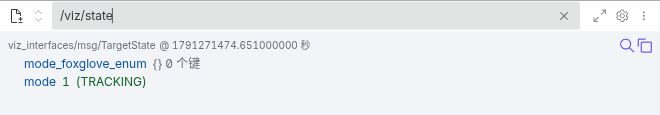
\includegraphics[width=0.9\linewidth]{images/ros2_foxglove_enum_revised.jpg}
  \caption{Humble 构建上述接口后发布 mode=1，Raw Messages 同时显示数字 1 与 TRACKING；常量定义字段本身仍是空对象。}
  \label{fig:ros2-foxglove-enum}
\end{figure}
\end{note}

\subsubsection{Foxglove Plot：字段路径与数值换算}
\label{sec:ros2-foxglove-plot}

先在 Plot 中把 X-axis value type 选为 Timestamp，添加两个 Series，Y-value 分别填 \path{/viz/signal.data} 和 \path{/viz/pose.pose.position.x}。Foxglove 用点号进入字段，与刚才 rqt\_plot 的斜线路径不同。输入路径时可以使用字段补全，也可以在 Raw Messages 中先确认字段层级，再复制相应路径。

\begin{example}[不用改发布程序，把四元数画成角度]
给 Plot 再加一条曲线，Y-value 填下面的完整路径。\texttt{.@rpy} 放在四元数对象后，转换结果还有 roll、pitch、yaw 三个字段，我们继续选 yaw，再把弧度换成角度。
\begin{lstlisting}[language={}]
/viz/pose.pose.orientation.@rpy.yaw.@degrees
\end{lstlisting}
这里只有 yaw 旋转，曲线会不断增长，到角度的表示边界后跳回另一端；这次跳变来自角度的周期表示，不表示目标突然转了整圈。真实三维姿态涉及旋转顺序，\texttt{.@rpy} 按 XYZ 内禀顺序转换，\texttt{.@ypr} 按 ZYX 顺序转换，先确认你要比较的角度定义。直接画 orientation.z 得到的只是四元数的一个分量。

这些后缀是 Foxglove 的字段路径函数（当前文档称 FoxQL），对查看器里的值做变换。常用写法整理如下，具体函数和版本差异可查\href{https://docs.foxglove.dev/docs/visualization/foxql}{官方函数说明}。
\begin{center}
\begin{tabular}{p{0.35\linewidth}p{0.57\linewidth}}
\toprule
字段后缀 & 用法与条件\\
\midrule
\nolinkurl{.@rpy.yaw}、\nolinkurl{.@rpy.roll} & 从 x/y/z/w 四元数中取欧拉角，结果是弧度；可继续选 pitch。\\
\nolinkurl{.@degrees}、\nolinkurl{.@radians} & 弧度转角度、角度转弧度，输入单位要先确认。\\
\nolinkurl{.@abs}、\nolinkurl{.@negative} & 取绝对值、改变符号，方便检查误差幅值或轴向。\\
\nolinkurl{.@mul(1000)}、\nolinkurl{.@div(1000)} & 乘除常数，例如米转毫米、毫秒转秒。\\
\nolinkurl{.@add(1)}、\nolinkurl{.@sub(1)} & 加减常数，用于比较带固定偏置的量。\\
\nolinkurl{.@norm} & 对 x/y/z 向量或数值数组取欧氏模长，例如速度大小。\\
\nolinkurl{.@length} & 取数组长度，例如 Path 中当前保存的位姿数。\\
\nolinkurl{.@sqrt}、\nolinkurl{.@log10} & 平方根、十进制对数，先检查输入取值范围。\\
\nolinkurl{.@sin}、\nolinkurl{.@cos} & 三角函数，输入使用弧度。\\
\nolinkurl{.@delta} & 相邻样本的值之差，结果单位与原值相同。\\
\nolinkurl{.@derivative} & 相邻样本的差除以时间差，单位变成原单位每秒。\\
\nolinkurl{.@timedelta} & 相邻样本之间的时间差，单位是秒。\\
\bottomrule
\end{tabular}
\end{center}

\Needspace{8\baselineskip}
在本例中可以直接试下面几条路径：
\begin{lstlisting}[language={}]
/viz/signal.data.@abs
/viz/pose.pose.position.x.@mul(1000)
/viz/twist.twist.linear.@norm
/viz/path.poses.@length
/viz/pose.pose.position.x.@derivative
/viz/pose.pose.position.x.@timedelta
\end{lstlisting}
第一条把正弦波的负半轴翻上来；第二条把米换成毫米；第三条的速度大小接近 1 m/s；第四条增加到 120 后保持不变。第五条可以与 \path{/viz/twist.twist.linear.x} 对照，差分会有离散采样误差；第六条约为 0.1 秒。函数可以顺序组合，例如先 \texttt{.@rpy.yaw} 再 \texttt{.@degrees}，每一步都接收上一步的结果。

取数组中的一项用 \texttt{[0]}，取全部用 \texttt{[:]}，例如 \path{/viz/markers.markers[0].pose.position.x}。把许多数组元素一起画进一条时间曲线，可能会在每个时刻连出一堆折线；想观察一个目标时，先选固定项或按 id 过滤。图形对象的数组顺序可能变化，工程里更可靠的路径是 \path|/viz/markers.markers[:]{id==0}.pose.position.x|，先在 Raw Messages 核对筛选结果，再加到曲线。

\begin{note}
\texttt{.@delta}、\texttt{.@derivative}、\texttt{.@timedelta} 需要 Timestamp 横轴，不能用在 XY 或 Array index 横轴上；一条函数链最多用一个这样的时间序列函数。函数缺失或路径报错时先检查客户端版本。用差分看角速度时，还要处理角度绕回和噪声，否则 $179^\circ$ 到 $-179^\circ$ 的表示变化会产生很大的假尖峰。
\end{note}

\end{example}

\subsubsection{Foxglove Plot：时间对齐与两点测量}
\begin{example}[按同一种时间来源比较曲线与轨迹]
消息里有正确填写的 \texttt{header.stamp} 时，我们\textbf{优先用它来画曲线}。在 Series 的 Timestamp 设置中选择 Header stamp（中文界面为“ROS 头时间戳”），这样比较的是数据采集或生成的时刻。传输和处理有延迟时，两条本来同时采集的数据也能按原来的时间对齐；\texttt{.@derivative} 和 \texttt{.@timedelta} 同样使用这里选定的时间来源。

本例的 pose、twist 和 path 都有 header，因此共同选 Header stamp；Float64 没有 header，signal 使用 Log time。这里先用它对照波形；真要精确比较 signal 与位姿的相位，就给自定义信号消息增加 Header，在同一次采样填入相同时间，再统一选 Header stamp。Log time 在实时连接中表示消息被接收的时刻，在录制文件中是原来的记录时刻，适合从接收侧观察消息间隔。先在 Raw Messages 确认 header.stamp 有效、持续更新，并核对比较对象使用同一种时钟；全为零或填错时，先修发布端。比较多条曲线时别混用采集时间与接收时间，采样频率不一样时也别把提示框中的最近一次值当成同一时刻的新样本。

现在点 Plot 工具栏中的 Inspection（两点检查）工具，依次选择两个曲线点。图例区域会显示两点的坐标以及沿各轴的差值：时间曲线的 $\Delta x$ 是时间间隔，$\Delta y$ 是数值变化。比如同一条正弦曲线的两个相邻峰值，间隔应该约为 $2\pi$ 秒。按 Esc 取消已选点，再按一次退出工具。

\begin{figure}[H]
  \centering
  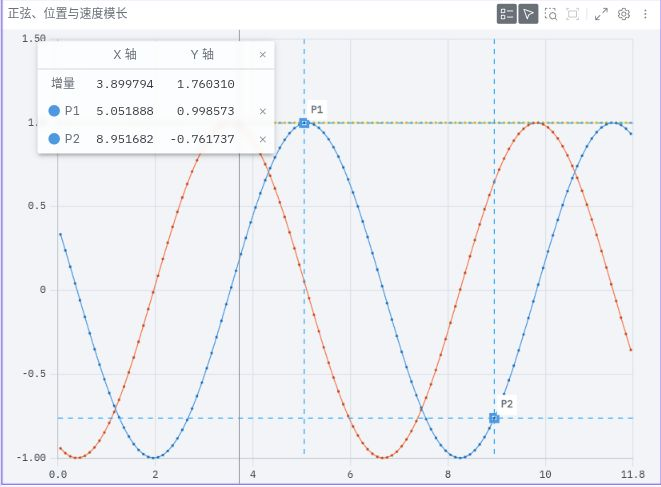
\includegraphics[width=0.96\linewidth]{images/ros2_foxglove_plot_measure_revised.jpg}
  \caption{打开点检查后选中 P1、P2；本次实测横轴差约 3.900 s，正弦值差约 1.760，两项单位分别读。}
  \label{fig:ros2-foxglove-plot-measure}
\end{figure}

还可以把 X-axis value type 改成 Expression，X-value 填 \path{/viz/pose.pose.position.x}，Y-value 填 \path{/viz/pose.pose.position.y}，Time range 选 All，Axis scales 选 1:1。这样会画出平面上的圆轨迹，两轴单位都是米，用两点检查还可以读到直线距离。时间曲线的横轴是秒、纵轴是米时，沿两轴的差值各有用途，把它们合成一个“距离”就没有物理意义了。

\begin{figure}[H]
  \centering
  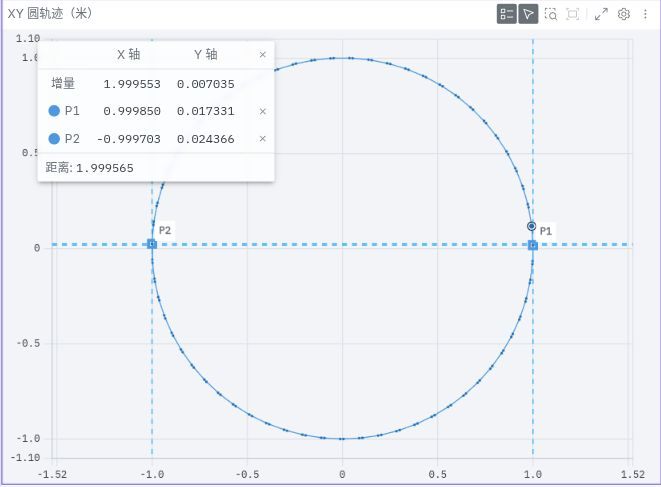
\includegraphics[width=0.96\linewidth]{images/ros2_foxglove_xy_measure_revised.jpg}
  \caption{XY 图的两轴都取位置，等比例显示圆轨迹；选取接近相对的两个采样点，实测距离为 1.999565 m。}
  \label{fig:ros2-foxglove-xy-measure}
\end{figure}

滚轮缩放、拖动平移，选中面板后按 r 或双击重置视图；按 z 进入框选缩放。按住 Alt 只缩放横轴，Shift 只缩放纵轴。曲线比较多时给 Series 改一个带单位的 Label，必要时分到不同面板或第二纵轴；右键图表导出 CSV，保留字段路径、时间来源和单位，后面复查才知道画的是什么。完整操作见\href{https://docs.foxglove.dev/docs/visualization/panels/plot}{官方 Plot 面板说明}。
\end{example}

\begin{exercise}\label{ex:v2-ros-foxglove-plot}
画出 yaw 的角度曲线、速度模长和相邻消息时间差。用 Inspection 测量正弦曲线两个相邻峰值的间隔，再用 XY 图测量圆上相对两点的距离。记录表达式、时间来源和单位，解释为什么时间曲线上的两轴差值不能直接合成空间距离。
\end{exercise}

\subsubsection{Foxglove 的 Image：把检测框与原图对上}
\label{sec:ros2-image-annotations}

先在 Image 面板选择 \path{/viz/image}。绿色色块应该和 rqt 中一样，但检测框不会因为你有一条“包含四个点的普通消息”就自动出现。Foxglove 识别的是明确的标注类型，这里使用 \path{foxglove_msgs/msg/ImageAnnotations}，里面按用途放 circles、points 和 texts。它们属于像素坐标，原点在图像左上角，x 向右、y 向下，和刚才以米为单位的三维 Marker 分开填写。

\begin{example}[原图不动，框、中心与标签单独发布]
下面是完整的 annotations.py。四个角点组成 LINE\_LOOP，查看器自动连接最后一点与第一点；圆和文字分别用自己的标注类型，颜色仍要填 alpha。
\Needspace{12\baselineskip}
\lstinputlisting[language=Python,basicstyle=\ttfamily\fontsize{9.5}{11.5}\selectfont,caption={annotations.py：二维框、中心和标签}]{examples/ros2/visualization-demo/annotations.py}

box 的 points 是像素位置，thickness 是像素线宽，fill\_color.a 默认 0，框内保持透明；CircleAnnotation 的 diameter 是直径。TextAnnotation 的 position 是文字区域的左下锚点，整个图像坐标仍以左上为原点，font\_size 用像素表示。这里的 confidence 是为展示准备的固定文本，示例没有执行目标识别。

回到 Image 的 Panel 设置，在可用标注话题中勾选 \path{/viz/annotations}，确认它显示为 ImageAnnotations，再打开 General 中的 Sync timestamps。你应看到黄色框包住绿色色块，红色小圆标出中心，文字在框上方；关闭标注话题时，原图仍保留色块。原图可以选择适合窗口、1:1 像素等缩放方式，查看像素值时把显示缩放与原图坐标分清。

\begin{figure}[H]
  \centering
  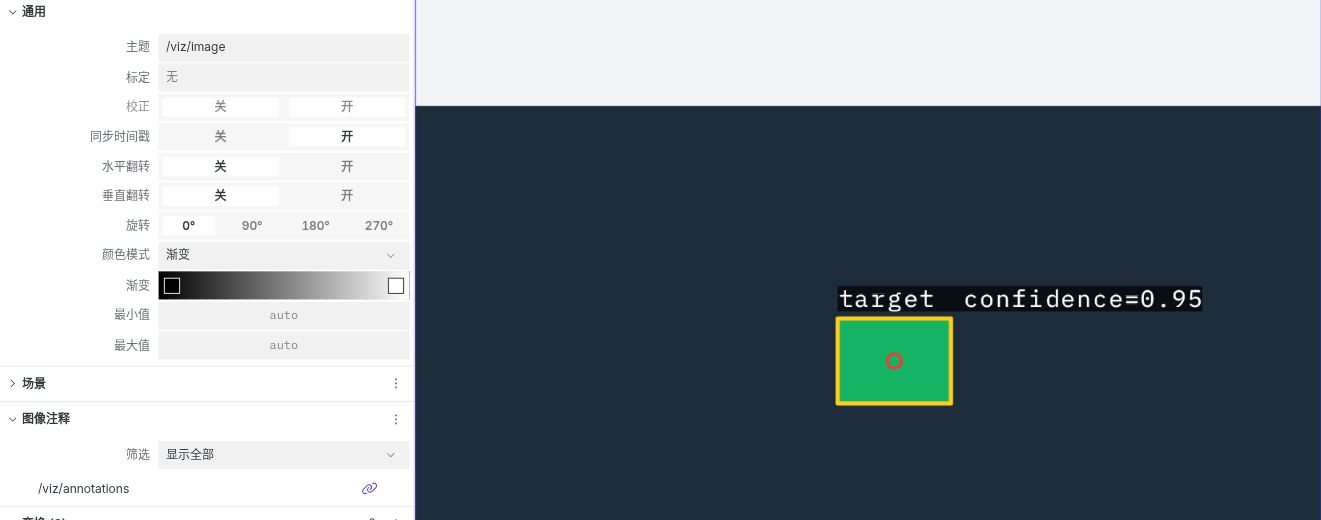
\includegraphics[width=0.96\linewidth]{images/ros2_foxglove_image_sync_revised.jpg}
  \caption{Image 面板打开时间戳同步，并启用 /viz/annotations；黄色框、红色中心与文字和原图一起显示。}
  \label{fig:ros2-foxglove-image-sync}
\end{figure}

同步匹配的是消息时间戳，不是“同样每秒发十次”。本例在同一次回调中把 image.header.stamp 传给每一个标注，新版 ImageAnnotations 的顶层 timestamp 也使用同一个值。算法稍晚算完时，仍把结果关联到输入图像的 header.stamp，别换成处理完成时的当前时间。旧版消息没有顶层 timestamp 时，客户端会使用标注元素的 timestamp，因此代码也给每一项填入同一时间。

打开同步后画面不更新，先检查是否只有框没有图、某个已勾选的标注话题停发，或两边时间差了一点；这里要求时间戳完全一致。本例把标注统一晚填 50 ms 后，客户端显示“等待同步消息”，恢复原图时间后又能正常更新。把检测框坐标按另一种图像尺寸计算，或者把归一化的 0 到 1 坐标直接填成像素，也会让框挤到角落里。前面合成图像的位移有意与圆运动分别定义，这些二维框用于演示像素标注，没有用相机模型把三维位置投影进图像。

真实相机的 CompressedImage 也可以在 Image 面板显示；需要叠加三维物体投影时，还要提供 CameraInfo 中的内参与坐标变换。单纯显示二维框不要求 CameraInfo；投影与畸变处理留到相机标定章节，别为了能看到框就随便填一份内参。像素标注、同步和投影的设置见\href{https://docs.foxglove.dev/docs/visualization/panels/image}{Image 面板说明}，字段类型见\href{https://docs.foxglove.dev/docs/sdk/schemas/image-annotations}{ImageAnnotations 定义}。
\end{example}

\begin{exercise}\label{ex:v2-ros-image-annotations}
把框的线宽改成 5 像素、中心圆直径改成 20 像素，保存一帧带标注的画面。再临时把所有标注时间戳加 50 ms，观察开启同步后的现象，恢复代码后重启。说明显示错误来自坐标、时间还是图像编码，并给出核对办法。
\end{exercise}

\subsubsection{Foxglove 3D：场景实体与空间测量}
\label{sec:ros2-foxglove-3d}

在 3D 的 Panel 设置里把 Display frame 选为 map，打开 TF、/viz/pose、/viz/path 与 /viz/markers，你应看到和 RViz2 对应的目标及轨迹。点一个对象可以查看其话题、编号与字段，再打开 Raw Messages 查同一对象。想跟着目标观察时可以选择 target 为跟随的坐标系；先用 map 看清整个运动，再切换视角，避免把相机视角的变化误认成目标运动。

\begin{example}[一个 SceneEntity 组合多个三维图形]
ROS Marker 可以直接共用，Foxglove 也提供原生的 \path{foxglove_msgs/msg/SceneUpdate}。它的 entities 中每个 SceneEntity 都有 frame\_id、timestamp、字符串 id、lifetime 和 frame\_locked，再把方块、箭头、线、文字等放到 cubes、arrows、lines、texts 数组中。下面的 scene.py 在同一个实体里组合一个方块和一段文字。
\lstinputlisting[language=Python,basicstyle=\ttfamily\fontsize{9.5}{11.5}\selectfont,caption={scene.py：把多个图元组合成一个三维实体}]{examples/ros2/visualization-demo/scene.py}

在 3D 中关闭 /viz/markers，打开 /viz/scene，绿色方块与文字就来自这份消息。cube 的 pose 给位置与朝向，size 给三轴尺寸；text.billboard 让文字朝向查看相机，scale\_invariant 让 font\_size 按屏幕像素表示，否则字高按世界坐标中的尺寸解释。本例每次沿用 target 这个 id，在同一话题中替换已有实体，lifetime 为 0.5 秒，停止更新后会过期。

SceneUpdate.deletions 可以放 SceneEntityDeletion，填写新时间、type 为 MATCHING\_ID、id 为 target，删除同话题中的旧实体；ALL 清理该话题已有实体。需要持续删除时先停止该实体的发布，否则下一条 entities 更新又会加回来。Marker 使用 ns/id 与 action，SceneUpdate 使用实体 id 和独立的 deletions 数组，各按自己的消息定义填写。RViz2 的默认显示不直接识别 SceneUpdate，使用哪种接口也要考虑队友的查看工具。

再点 3D 右侧的 Measure 工具，选择两个点读距离。默认点击落在地面平面上，测量实体表面或点云点时按住 Alt 启用吸附（macOS 用 Option），确认端点确实贴在对象上。世界坐标单位为米，量一个已知 0.25 m 的方块可以帮助检查尺度。测到的只是当前展示的几何结果；坐标变换或尺寸填错时，尺子也会跟着量错。图形接口与测量控制分别见\href{https://docs.foxglove.dev/docs/sdk/schemas/scene-update}{SceneUpdate 定义}和\href{https://docs.foxglove.dev/docs/visualization/panels/3d}{3D 面板说明}。
\end{example}

\subsubsection{MCAP 录制与回放：把一次观察留下来}
\begin{example}[录一段，再慢慢找不对劲的时刻]
实时数据太快时，我们先把它留下。Humble 默认常用的 db3 不保存全部自定义消息定义，这里安装 MCAP 存储插件，并明确使用 \texttt{-s mcap}。保持数据源运行，在新的工作目录中录制本例的话题：
\par\medskip\noindent\begin{minipage}{\linewidth}
\begin{tbash}
sudo apt install ros-humble-rosbag2-storage-mcap
mkdir -p ~/ros_viz_recordings
cd ~/ros_viz_recordings
ros2 bag record -s mcap -o viz_demo_01 \
  /viz/signal /viz/pose /viz/twist /viz/path /viz/image \
  /viz/markers /viz/annotations /viz/scene /tf
\end{tbash}
\end{minipage}\par\smallskip
录十几秒后按 Ctrl+C，让录制器正常收尾；输出目录要用尚不存在的名字，第二次可以改成 viz\_demo\_02。先用 \texttt{ros2 bag info viz\_demo\_01} 核对话题和消息数量，再关闭实时连接，在 Foxglove 用 Open local file(s) 打开目录里的 \texttt{.mcap} 文件，并恢复自己的布局。文件从容器产生时，先找到宿主能访问的实际路径。

回放可以暂停、拖动时间线、降低播放速度。点 Plot 上的一个时间点，回放位置会跳到那里，Image 和 3D 也跟着显示该时刻附近的数据。再用两点检查量周期、位置变化或处理异常持续多久；图像与标注开启同步时，查看同一帧的对应关系。实时模式没有“跳到刚才那一刻”的录制时间线，这也是我们要留下文件的原因。

\begin{figure}[H]
  \centering
  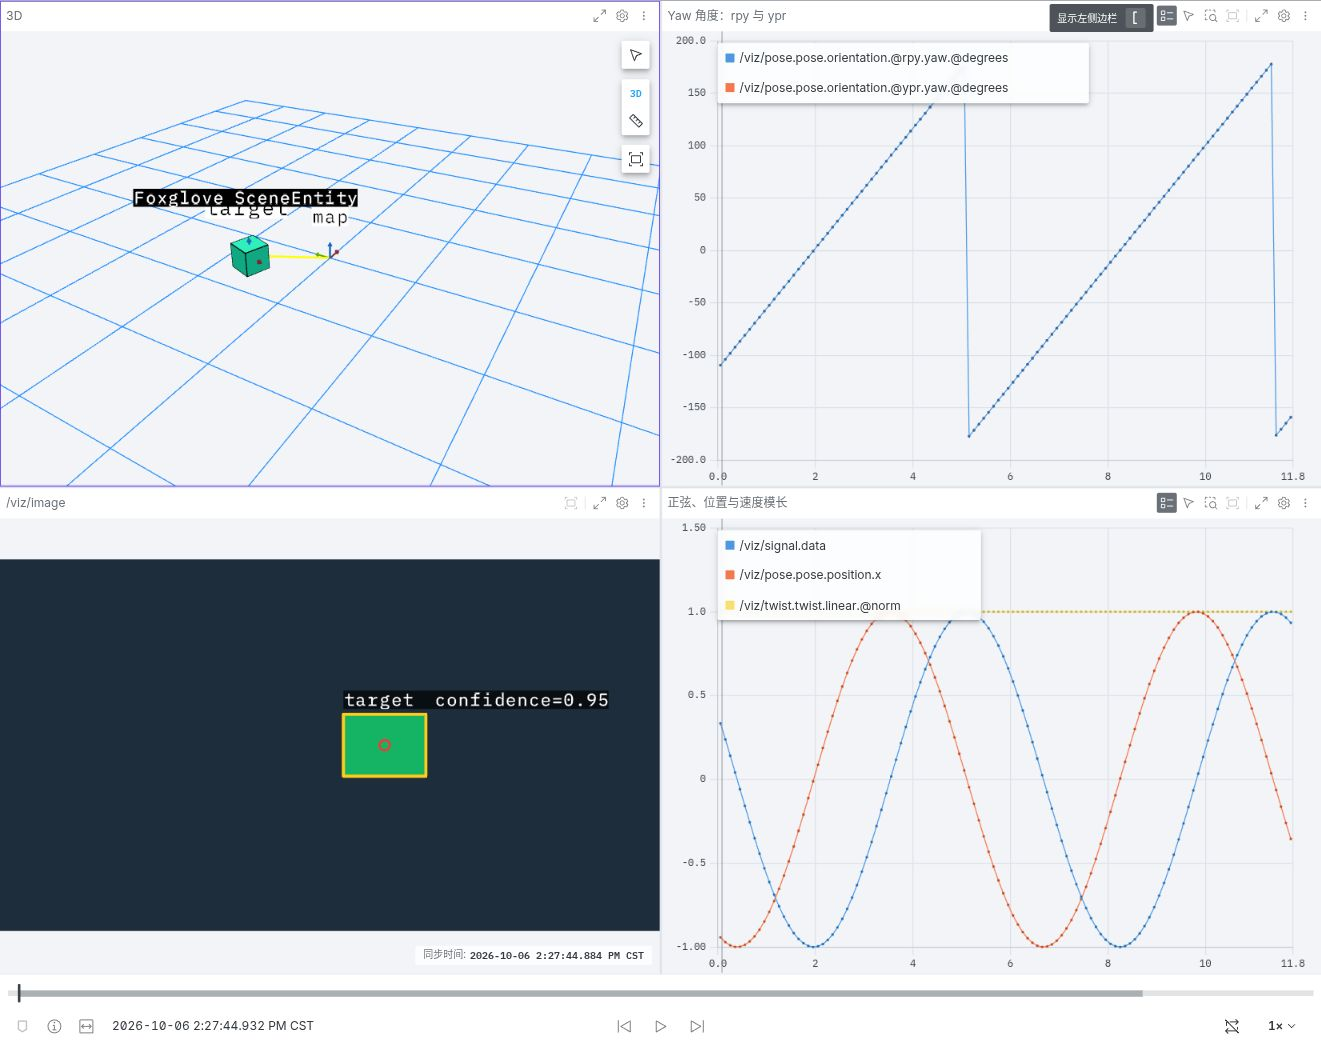
\includegraphics[width=0.98\linewidth]{images/ros2_foxglove_replay_revised.jpg}
  \caption{同一份 MCAP 的暂停画面：左侧对照 SceneEntity 和原图标注，右侧查看 yaw、位置与速度模长；下方时间线选择要复查的时刻。}
  \label{fig:ros2-foxglove-replay}
\end{figure}

录制与显示支路也会消费带宽、CPU 和存储。本节 640×360、10 Hz 的数据用来练工具；接上高帧率相机时，按后面的大图像链路章节安排降频观测支路，再检查显示或录制是否影响主链路。
\end{example}

\begin{conclusion}
现在我们有了几种互相补充的观察方式：先用消息字段确认输入，再用曲线看变化，用图像核对像素与标注，用三维场景核对坐标与尺寸，最后把有问题的过程录下来回放。保存画面时，也把话题、字段路径、时间来源、单位与显示配置留下来，队友才能复查你看到的现象。
\end{conclusion}

\begin{exercise}\label{ex:v2-ros-viz-replay}
保存一份包含 Plot、Image 和 3D 的布局，录制至少 10 秒 MCAP，重新打开文件。用同一时间点对照位姿曲线、目标图形和原图标注；提交布局、录制文件与一项测量结果，并说明这里哪些数据是合成的、哪些功能仍需接入实际相机后验证。
\end{exercise}


\section{构建工具与环境排障}
% 工程实践：以 Ubuntu 22.04 / ROS2 Humble 为主。
\subsubsection{先检查环境，再检查代码}
\label{sec:ros2-environment}

刚才节点已经跑起来了，不过你很快会遇到另一种问题：终端能运行，IDE 却说找不到包，或者明明改了源码，启动后还是昨天的输出。这时候先别急着改 C++，我们先看看程序到底用了哪套环境。系统安装称为底层工作空间（underlay），自己的安装目录称为覆盖工作空间（overlay）；先加载底层，再加载覆盖层，同名包就可能被后者覆盖。

\begin{center}
\begin{tabular}{p{0.40\textwidth}p{0.52\textwidth}}
\toprule[1.5pt]
变量 & 作用 \\
\midrule[1pt]
\nolinkurl{ROS_VERSION / ROS_DISTRO} & 判断当前终端所加载的 ROS 版本线索。\\
\texttt{AMENT\_PREFIX\_PATH} & ament 查找已安装包的前缀。\\
\texttt{CMAKE\_PREFIX\_PATH} & CMake 查找依赖的前缀。\\
\nolinkurl{PYTHONPATH / LD_LIBRARY_PATH} & Python 模块与动态库搜索路径。\\
\texttt{ROS\_DOMAIN\_ID} & 通信域编号；通信双方需要一致。\\
\texttt{ROS\_LOCALHOST\_ONLY} & DDS 实验中设为 1 时只与本机通信；Zenoh 的连接范围见后文配置。\\
\texttt{RMW\_IMPLEMENTATION} & 选择已经安装的中间件实现。\\
\bottomrule[1.5pt]
\end{tabular}
\end{center}

\begin{example}[确认终端实际使用的包]
完成前面的工作空间练习后，在新终端执行：
\par\medskip\noindent\begin{minipage}{\linewidth}
\begin{tbash}
source /opt/ros/humble/setup.bash
source ~/ros2_ws/install/setup.bash
printenv ROS_VERSION ROS_DISTRO AMENT_PREFIX_PATH
ros2 pkg prefix my_package
ros2 pkg executables my_package
\end{tbash}
\end{minipage}\par\smallskip
应显示 ROS 版本 2、发行版 humble，以及自己工作空间中的包安装前缀。若路径指向别的工作空间，先修正加载顺序；若找不到包，检查构建是否成功、包名是否一致。
\end{example}

\subsubsection{通信域与发现范围：只与自己的节点通信}
域编号用于把通信分组，不同域的节点之间不会互相通信。

\begin{example}[临时启用本机通信并恢复]
在两个终端分别执行下面的环境设置，然后分别运行 talker 与 listener。域 42 是这次练习的分组编号，实验室已有分配时换成你的编号：
\par\medskip\noindent\begin{minipage}{\linewidth}
\begin{tbash}
source /opt/ros/humble/setup.bash
export ROS_DOMAIN_ID=42
export ROS_LOCALHOST_ONLY=1
ros2 daemon stop
# 终端 A
ros2 run demo_nodes_cpp talker
# 终端 B
ros2 run demo_nodes_cpp listener
\end{tbash}
\end{minipage}\par\smallskip
应看到本机 listener 收到消息。在另一台机器使用相同域和普通网络发现时，无法收到本次本机发布的数据。

按 Ctrl+C 停止两个节点。在两个终端分别执行下列命令，再重新启动节点，恢复默认域和普通发现范围：
\par\medskip\noindent\begin{minipage}{\linewidth}
\begin{tbash}
unset ROS_LOCALHOST_ONLY ROS_DOMAIN_ID
ros2 daemon stop
\end{tbash}
\end{minipage}\par\smallskip
\end{example}

Humble 的本机实验使用 \texttt{export ROS\_LOCALHOST\_ONLY=1}。跨机器通信时，两端先取消本机限制，再设置相同域编号并重启节点与 daemon。

\begin{note}
建议大家调车时，记得设置只在本地通信。曾经学长在调试场地发现明明没启动自瞄的车居然还能收到图像消息，沉思了半个小时，差点要怀疑人生了，最后发现自己的手机非常的烫，才意识到是自己开了热点，所有车都在同一个域里互相通信了。
\end{note}

\paragraph*{用环境变量切换中间件}
\texttt{RMW\_IMPLEMENTATION} 用来选择已经安装的中间件实现。例如 Humble 默认的 Fast DDS 对应 \nolinkurl{rmw_fastrtps_cpp}。先停止旧节点，再在启动节点的两个终端分别设置：
\par\medskip\noindent\begin{minipage}{\linewidth}
\begin{tbash}
export RMW_IMPLEMENTATION=rmw_fastrtps_cpp
ros2 daemon stop
\end{tbash}
\end{minipage}\par\smallskip
重新启动节点后，新进程才会使用这个选择；用 \texttt{unset RMW\_IMPLEMENTATION} 可以恢复默认实现。安装其他实现后，改这个变量就能切换。具体安装、配置和对照实验留到第\ref{sec:ros2-rmw-selection}节，再结合大图像链路一起看。

\begin{conclusion}
\begin{itemize}
\item 找不到包：先确认构建、安装和环境加载，再修改代码。
\item 看不到节点：检查域、发现范围和 RMW，再检查 QoS 与接口。
\item 改了环境：重启相关节点与 daemon；变量只影响继承它的新进程。
\item 域与发现范围负责通信组织；认证和访问控制需要另行配置。
\end{itemize}
\end{conclusion}

\begin{exercise}
\label{ex:v2-ros-domain}
让本机 talker 使用域 42、listener 使用域 43，观察现象；把两端统一为 42 后重新启动并验证。写出恢复环境需要处理的进程和变量。
\end{exercise}

\Needspace{18\baselineskip}
\subsubsection{ament、colcon 与可复现的小工程}
\label{sec:ros2-ament}

到这里你已经接触了好几个名字：CMake、ament、colcon、rosdep。它们看起来都和“编译”有关，其实各自负责一段。我们下来详细介绍它们：CMake 描述单个 C++ 包怎样编译和安装，ament 提供 ROS2 的依赖、安装索引和导出约定，colcon 按依赖顺序构建工作空间中的多个包，rosdep 则根据依赖键安装系统依赖。

\begin{example}[建立共用教学包]
这次我们用一个简单心跳节点把依赖、测试、参数和启动文件串起来。源码在本卷 \path{examples/ros2/training_tools}，与前面的 my\_package 相互独立。先看看需要哪些文件：
\par\medskip\noindent\begin{minipage}{\linewidth}
\begin{lstlisting}[language={}]
training_tools/
  package.xml
  CMakeLists.txt
  src/heartbeat.cpp
  test/test_interval.cpp
  config/heartbeat.yaml
  launch/basic.launch.py
  launch/heartbeat.launch.py
  launch/team.launch.py
  launch/multi.launch.py
  launch/checked.launch.py
  cmake/Auto.cmake       # 只在自动宏实验时替换构建规则
\end{lstlisting}
\end{minipage}\par\smallskip
你可以把这个目录复制到 \path{~/ros2_ws/src}。也可以按下面逐个保存文件，先建目录：
\par\medskip\noindent\begin{minipage}{\linewidth}
\begin{tbash}
mkdir -p ~/ros2_ws/src/training_tools/{src,launch,config,test}
cd ~/ros2_ws/src/training_tools
\end{tbash}
\end{minipage}\par\smallskip
保存 \texttt{package.xml}。这份文件是依赖清单，里面写明了这个包的名字，版本，描述，维护者，许可证类型。不过这些对我们的实际使用都不是很重要，我们需要掌握的是里面具体写出依赖的部分，需要把这个包和其他包的依赖关系写清楚。否则在编译时可能导致先后顺序弄错而无法编译。\nolinkurl{<buildtool_depend>} 声明 ament 等构建工具，\nolinkurl{<build_depend>} 声明构建依赖，\nolinkurl{<build_export_depend>} 声明下游编译所需依赖，\nolinkurl{<exec_depend>} 声明运行依赖，\nolinkurl{<test_depend>} 声明测试依赖。\nolinkurl{<depend>} 合并普通依赖的构建、导出与运行三种用途。对于初学者而言，只要使用最后一个\nolinkurl{<depend>}就可以了。
\Needspace{23\baselineskip}
\par\medskip\noindent\begin{minipage}{\linewidth}
\lstinputlisting[frame=single,language=XML,caption={training\_tools/package.xml}]{examples/ros2/training_tools/package.xml}
\end{minipage}\par\smallskip
接下来保存 \nolinkurl{src/heartbeat.cpp}。构造函数读出 text 参数，创建发布者，再让定时器每 200 毫秒发一次消息。句柄保存在成员中；lambda 捕获 text 的值，所以参数只在启动时读取一次，改变文本实验时要重启节点。
\Needspace{35\baselineskip}
\par\medskip\noindent\begin{minipage}{\linewidth}
\lstinputlisting[frame=single,basicstyle=\ttfamily\footnotesize,language=C++,caption={heartbeat 的完整节点实现}]{examples/ros2/training_tools/src/heartbeat.cpp}
\end{minipage}\par\smallskip
然后保存 \texttt{CMakeLists.txt}。它找到清单里声明的依赖，编译 heartbeat，再安装程序和 Launch、YAML 资源。测试文件在下面提供，手工建包时先关闭测试，文件齐了再开启。
\par\medskip\noindent\begin{minipage}{\linewidth}
\lstinputlisting[frame=single,language=cmake,caption={手动声明依赖与安装规则}]{examples/ros2/training_tools/CMakeLists.txt}
\end{minipage}\par\smallskip
通用构建形式为 \texttt{colcon build [包选择选项] [构建选项]}：
\begin{center}
\begin{tabular}{p{0.42\textwidth}p{0.50\textwidth}}
\toprule[1.5pt]
参数 & 作用 \\
\midrule[1pt]
\texttt{--packages-select 包名} & 仅构建选定包，依赖需已可用。\\
\texttt{--packages-up-to 包名} & 构建目标及工作空间中的递归依赖。\\
\texttt{--symlink-install} & 在可用处采用符号链接安装。\\
\texttt{--cmake-args 参数} & 向 CMake 传递配置参数。\\
\bottomrule[1.5pt]
\end{tabular}
\end{center}
其余选项查询 \texttt{colcon build --help}。

一般来说，我们使用这条命令：
\par\medskip\noindent\begin{minipage}{\linewidth}
\begin{tbash}
colcon build --symlink-install --cmake-args -DCMAKE_BUILD_TYPE=Release
\end{tbash}
\end{minipage}\par\smallskip
它会构建工作空间中所有包，并在可用处使用符号链接。使得我们修改参数时不必重新编译。Release 模式优化编译速度和运行效率。为了方便起见，我们可以在 \texttt{~/.bashrc} 或 \texttt{~/.zshrc} 中写一个别名：
\par\medskip\noindent\begin{minipage}{\linewidth}
\begin{tbash}
alias cb='colcon build --symlink-install --cmake-args -DCMAKE_BUILD_TYPE=Release'
\end{tbash}
\end{minipage}\par\smallskip

下面先关闭测试，把节点跑通。rosdep 第一次使用时需初始化：系统尚无默认源列表时执行一次 \texttt{sudo rosdep init}，然后用普通用户执行 \texttt{rosdep update}；已经初始化就跳过 init。接下来让它从清单中安装缺少的依赖：
\par\medskip\noindent\begin{minipage}{\linewidth}
\begin{tbash}
cd ~/ros2_ws
source /opt/ros/humble/setup.bash
rosdep install --from-paths src --ignore-src -r -y
colcon build --packages-select training_tools --cmake-args -DBUILD_TESTING=OFF
source install/setup.bash
ros2 run training_tools heartbeat
\end{tbash}
\end{minipage}\par\smallskip
另一终端加载相同环境后运行 \texttt{ros2 topic echo /status}，应持续收到 ready。消息发布约 5 Hz。
\end{example}

\Needspace{18\baselineskip}
\subsubsection{自动依赖、库导出与构建测试}
也许你已经觉得CMake里面的内容实在是冗长，每个包都需要 \nolinkurl{find_package}，然后\nolinkurl{target_link_libraries}，这样写一大串。
别担心， \texttt{ament\_cmake\_auto} 可以轻松地帮你减少重复声明。
它依据清单寻找依赖。
注意第三方库的 rosdep 键与 CMake 名称可能不同，例如OpenCV通过 \verb|rosdep resolve opencv2| 查询依赖，而 CMake  需要使用 \verb|find_package(OpenCV REQUIRED)|。这种时候Cmake里面的 \verb|find_package| 还是需要手动写的。

\begin{example}[同一个包改用 ament 自动宏]
在 \texttt{package.xml} 中把构建工具依赖改为 \texttt{ament\_cmake\_auto}，保留 export 中的 \texttt{ament\_cmake} 构建类型。把本项目 \path{cmake/Auto.cmake} 的内容复制为包根目录的 CMakeLists.txt，完整规则如下：
\par\medskip\noindent\begin{minipage}{\linewidth}
\lstinputlisting[frame=single,language=cmake,caption={自动宏构建规则}]{examples/ros2/training_tools/cmake/Auto.cmake}
\end{minipage}\par\smallskip
重新执行 rosdep 安装和前例的构建、运行命令，行为应相同。下来大家在写自己的ROS包时，手动版本和自动版本二选一即可。
\end{example}

若包要供其他包链接，还需安装库和公开头文件。手动构建时，用 \nolinkurl{ament_export_targets} 导出目标，用 \nolinkurl{ament_export_dependencies} 导出依赖；自动宏可简化这些规则。

文件末尾调用 \nolinkurl{ament_package()}，自动版本则调用 \nolinkurl{ament_auto_package()}，完成包索引与配置生成。

组件化还需要代码中的 \nolinkurl{RCLCPP_COMPONENTS_REGISTER_NODE} 和 CMake 的 \nolinkurl{rclcpp_components_register_nodes} 注册。这些我们会在第\ref{sec:ros2-image-components}节会用完整的图像工程，把组件注册、Launch 布局与数据所有权接起来。

\begin{example}[把参数边界变成自动检查]
在 \nolinkurl{test/test_interval.cpp} 保存一个无硬件依赖的边界测试。
\Needspace{20\baselineskip}
\par\medskip\noindent\begin{minipage}{\linewidth}
\lstinputlisting[frame=single,language=C++,caption={独立的间隔边界测试}]{examples/ros2/training_tools/test/test_interval.cpp}
\end{minipage}\par\smallskip
在工作空间根目录执行：
\par\medskip\noindent\begin{minipage}{\linewidth}
\begin{tbash}
colcon build --packages-select training_tools --cmake-args -DBUILD_TESTING=ON
colcon test --packages-select training_tools
colcon test-result --verbose
\end{tbash}
\end{minipage}\par\smallskip
两组测试应通过。更多测试规则请查阅 \href{https://google.github.io/googletest/}{GTest官方文档}。
\end{example}

\begin{conclusion}
\begin{itemize}
\item 清单声明依赖；rosdep 安装系统依赖；CMake/ament 使用它们构建包。
\item colcon 组织多个包，安装后的索引让 ROS2 能查到可执行程序和资源。
\item 库的导出影响下游使用；只在本包编译成功还不够。
\item 自动宏减少重复配置。
\end{itemize}
\end{conclusion}
\begin{exercise}
\label{ex:v2-ros-ament}
说明为什么源目录已有 launch 文件，\texttt{ros2 launch} 仍可能找不到它。将上例合法间隔上限改为 500，同时修改边界测试并重新验证。
\end{exercise}

\section{Launch 启动配置与模块组合}
\subsubsection{Launch 入门：用一个文件启动节点}
\label{sec:ros2-launch}

你现在已经能手动启动节点了。不过真正上车时，相机、识别、串口各开一个终端，每个节点后面再跟一串参数，少打一个字，机器人就可能和你玩捉迷藏。启动文件（launch file）把这次需要运行的程序和配置记下来，下次用一条命令就能把它们重新启动。我们先让刚才的 heartbeat 跑起来，再逐步加上参数、命名空间和组合启动，最后看看需要按条件、按事件启动时怎么写。

ROS2 支持 Python、XML 和 YAML 格式的启动文件。本节使用 Python：基础配置可以直接写，后面需要循环、检查文件或处理事件时，也能沿着同一种写法继续扩展。启动文件用什么语言，和节点用什么语言没有关系；Python Launch 完全可以启动我们刚写好的 C++ 节点。

\paragraph*{先写一个只启动节点的文件}
Python 启动文件的入口是 \nolinkurl{generate_launch_description()}。ROS2 加载文件后会调用它，得到一个 \texttt{LaunchDescription}，也就是这次启动要执行的动作列表。动作（action）不一定是节点，还可以是设置环境、引入另一个启动文件或注册事件处理器。\texttt{Node} 来自 \texttt{launch\_ros}，是在通用启动系统之上增加了 ROS 节点配置的动作。

\begin{example}[把 ros2 run 写进启动文件]
继续使用前面的 training\_tools，不需要新建包。在包内保存 \nolinkurl{launch/basic.launch.py}，完整文件如下：
\par\medskip\noindent\begin{minipage}{\linewidth}
\lstinputlisting[frame=single,language=Python,caption={先启动一个心跳节点}]{examples/ros2/training_tools/launch/basic.launch.py}
\end{minipage}\par\smallskip
这里的 \texttt{package} 是功能包名，\texttt{executable} 是安装后的可执行程序名。它们对应 \texttt{ros2 run training\_tools heartbeat} 中的两个名字。\texttt{name} 覆盖节点在源码里设置的名字，程序名不变，节点名可以按启动需要另取。\texttt{output='screen'} 让子进程的输出显示在当前终端。

通用启动形式为 \texttt{ros2 launch 包名 文件名 [参数名:=值]}。前面的 CMake 已经安装整个 launch 和 config 目录，不过新增文件后仍要重新构建，让安装目录也有它。下面的命令在工作空间根目录执行：
\par\medskip\noindent\begin{minipage}{\linewidth}
\begin{tbash}
cd ~/ros2_ws
source /opt/ros/humble/setup.bash
colcon build --packages-select training_tools
source install/setup.bash
ros2 launch training_tools basic.launch.py
\end{tbash}
\end{minipage}\par\smallskip
另开一个终端，加载相同的底层和覆盖工作空间后检查：
\par\medskip\noindent\begin{minipage}{\linewidth}
\begin{tbash}
ros2 node list
ros2 topic echo /status std_msgs/msg/String --once
\end{tbash}
\end{minipage}\par\smallskip
你应能找到 \texttt{/heartbeat}，并收到一条 ready。回到启动终端按 Ctrl+C，Launch 会通知它管理的进程退出，再也不用逐个终端关节点了。
\end{example}

写 \texttt{Node(...)} 时，我们只是在描述“等会儿怎样启动”，并没有当场执行程序。把它放进返回的动作列表，启动系统才会处理它。这个区别后面会解释为什么参数不能直接当 Python 字符串用，也会解释为什么“写在前面”不等于“已经准备好了”。

\Needspace{18\baselineskip}
\subsubsection{Launch 配置：名字、YAML 与命令行参数}
刚才只有四个字段。真正开始连模块时，常用配置还包括下面这些：
\begin{center}
\begin{tabular}{p{0.25\textwidth}p{0.67\textwidth}}
\toprule[1.5pt]
字段 & 本节怎样使用 \\
\midrule[1pt]
\texttt{package / executable} & 找到已经安装的程序。\\
\texttt{name / namespace} & 设置节点名与命名空间，例如 \nolinkurl{/red/heartbeat}。\\
\texttt{parameters} & 传入参数字典、ROS 参数 YAML 文件，或把两者组合起来。\\
\texttt{remappings} & 用 \texttt{(原名, 新名)} 修改话题、服务等接口名称。\\
\texttt{output} & 设置子进程输出的去向；本节用 screen，日志出口见第\ref{sec:ros2-logging}节。\\
\texttt{additional\_env} & 在继承的环境上为这个进程增补环境变量。\\
\bottomrule[1.5pt]
\end{tabular}
\end{center}

先把三个“名字”分开：包名帮助 ROS2 找程序，节点名帮助你在计算图里找节点，话题名决定数据从哪里进、从哪里出。改节点名不会把它发布的所有话题一并改名。比如 heartbeat 源码里发布的是相对话题 \texttt{status}；加上 \texttt{namespace='red'}，完整名字就变成 \texttt{/red/status}。再写 \texttt{remappings=[('status', 'health')]}，最终发布到 \texttt{/red/health}。

这里的相对名字会跟着命名空间走，而以 \texttt{/} 开头的绝对名字从根开始。例如把重映射目标写成 \texttt{/health}，结果就是 \texttt{/health}，不会再加 red。相机驱动发布 image\_raw，识别节点订阅 image，也可以通过重映射把它们接到同一个名字。不过你要分别核对两端的最终话题、类型和 QoS，Launch 不会替你修好接口不匹配的问题。

\paragraph*{先放进 YAML，再把常改的值留给命令行}
配置还少的时候，直接写 \texttt{parameters=[\{'text': 'ready'\}]} 就够用了。配置多起来之后，把它们放进 YAML 更方便比较和保存；经常随机器人或实验变化的几项，再通过启动参数（launch argument）从命令行传入。我们把这两种办法放在同一个例子里。

\begin{example}[保存配置，并在启动时覆盖它]
在 training\_tools 包内保存 \nolinkurl{config/heartbeat.yaml}：
\par\medskip\noindent\begin{minipage}{\linewidth}
\lstinputlisting[frame=single,language={},caption={心跳节点的 ROS 参数文件}]{examples/ros2/training_tools/config/heartbeat.yaml}
\end{minipage}\par\smallskip
\texttt{ros\_\_parameters} 下面才是节点参数。最外层的 \texttt{/**} 是通配节点键，让这份简单配置在节点改名或加命名空间后仍适用。若只想配置 \nolinkurl{/red/heartbeat}，也可以把这个键改成它的完整名字；名字不匹配时，文件虽然找到了，参数却不会落到你想配置的节点上。多节点系统也要留意通配键的范围，别把本来只给一个节点的配置发给其他节点。

接下来保存 \nolinkurl{launch/heartbeat.launch.py}。这次让 robot 控制命名空间，text 控制消息内容，params\_file 控制 YAML 路径：
\par\medskip\noindent\begin{minipage}{\linewidth}
\lstinputlisting[frame=single,basicstyle=\ttfamily\footnotesize,language=Python,caption={可从命令行配置的心跳启动文件}]{examples/ros2/training_tools/launch/heartbeat.launch.py}
\end{minipage}\par\smallskip

我们按使用顺序拆开看。\nolinkurl{get_package_share_directory('training_tools')} 从安装索引找到这个包的资源目录，\texttt{Path} 再把 config 和文件名接上。这样把工作空间搬到另一台机器，启动文件仍能找到随包安装的配置；不必把自己的 \path{/home/student/ros2_ws/src/...} 写死在里面。

\nolinkurl{DeclareLaunchArgument} 声明启动参数，给出默认值和说明。\nolinkurl{LaunchConfiguration('robot')} 则表示“执行到这里时，取 robot 的实际值”。它是一个替换对象（substitution），不是已经取出的 Python 字符串。声明参数不会自动修改节点：robot 必须接到 namespace 上，text 必须接到 parameters 上，它们才会影响这次运行。

\texttt{parameters} 中先放 YAML 路径，再放一个字典，后面的 text 会覆盖 YAML 中的同名项。因此，只运行这个文件而不传 text，收到的是默认启动参数 \texttt{ready from launch}，不是 YAML 中的 \texttt{ready from yaml}。这很适合“文件保存基础配置，命令行改少数常用项”的做法；如果你希望完全采用 YAML 的 text，就删除后面的 text 字典，让文件决定它。

最后，\texttt{ParameterValue(..., value\_type=str)} 明确告诉 Launch：text 要作为字符串传入。命令行传来的是文本，但 ROS 参数求值时可能把 true、123 这类内容解释成布尔量或整数，而 heartbeat 声明的 text 是字符串。把类型写清楚，可以避免“明明传了字，怎么说类型不对”的疑惑，真正的整数或布尔参数也可以相应指定 \texttt{int} 或 \texttt{bool}。

重新构建并加载环境后，先看这个文件允许传什么，再启动：
\par\medskip\noindent\begin{minipage}{\linewidth}
\begin{tbash}
ros2 launch training_tools heartbeat.launch.py --show-args
ros2 launch training_tools heartbeat.launch.py robot:=red text:=tracking
\end{tbash}
\end{minipage}\par\smallskip
\texttt{--show-args} 显示参数说明后退出，不会启动节点。第二条命令会启动 \nolinkurl{/red/heartbeat}，在另一终端检查：
\par\medskip\noindent\begin{minipage}{\linewidth}
\begin{tbash}
ros2 topic echo /red/health std_msgs/msg/String --once
ros2 param get /red/heartbeat text
ros2 node info /red/heartbeat
\end{tbash}
\end{minipage}\par\smallskip
应收到 tracking，参数查询也应显示 tracking，节点信息中能找到 \texttt{/red/health}。如果内容包含空格，把整个赋值参数加引号，例如 \texttt{'text:=ready for battle'}。若要使用另一份 YAML，传 \texttt{params\_file:=/实际路径/参数.yaml}。
\end{example}

\begin{note}
启动参数属于 Launch，节点参数属于运行中的 ROS 节点。\texttt{ros2 param get /red/heartbeat robot} 查不到本例的 robot，因为它只用来选择命名空间，并没有作为节点参数传入。\texttt{use\_sim\_time} 则是常见节点参数：需要模拟时钟的节点应一致设置，并有 \texttt{/clock} 来源；只给 Launch 声明一个同名参数不会自动配置所有节点。我们的 heartbeat 使用 \nolinkurl{create_wall_timer}，发布周期也不会因为设置模拟时间就自动改成模拟时钟。
\end{note}

\begin{exercise}
\label{ex:v2-ros-launch-basic}
把 basic 文件的节点名改为 pulse，确认程序仍叫 heartbeat、话题仍是 \texttt{/status}。然后用 heartbeat 启动文件传入 \texttt{robot:=blue text:=true}，查询完整节点名、最终话题名和 text 的参数类型。最后只在你的练习副本中删除覆盖 text 的字典，重新启动，说明消息为什么变回 YAML 中的内容。
\end{exercise}

\subsubsection{Launch 组合：引入子文件与条件启动}
现在 heartbeat 已经能独立启动了。系统里再加一个观测程序时，我们没必要在新的launch文件中复制刚才的配置，而是可以用 \nolinkurl{IncludeLaunchDescription} 引入它。相机、识别、串口以后也可以各保留一个启动文件，最外层的 bringup 文件只负责把它们组合起来。需要改相机参数时，就不用在一份几百行的文件里翻半天。

\begin{example}[按条件观测一条消息]
保存 \nolinkurl{launch/team.launch.py}。本例用 \texttt{ExecuteProcess} 启动 \texttt{ros2 topic echo}，它是一个普通命令行进程；启动 ROS 节点通常仍用 \texttt{Node}，这样不必自己拼接 ROS 参数。完整文件如下：
先导入需要的工具，并定义打印配置的辅助函数：
\par\medskip\noindent\begin{minipage}{\linewidth}
\lstinputlisting[frame=single,basicstyle=\ttfamily\footnotesize,language=Python,firstline=1,lastline=18,caption={team 的导入与辅助函数}]{examples/ros2/training_tools/launch/team.launch.py}
\end{minipage}\par\smallskip

接着在同一个文件里写出完整入口，把这些动作组合起来：
\par\medskip\noindent\begin{minipage}{\linewidth}
\lstinputlisting[frame=single,basicstyle=\ttfamily\footnotesize,language=Python,firstline=19,caption={team 的完整启动入口}]{examples/ros2/training_tools/launch/team.launch.py}
\end{minipage}\par\smallskip

入口函数里，我们先安排引入部分。目标文件交给 \nolinkurl{PythonLaunchDescriptionSource}，说明它是 Python 启动文件；\texttt{launch\_arguments} 把主文件的配置传给子文件。这里需要的是键值对序列，所以字典最后调用 \texttt{.items()}。主文件的 robot 接到了子文件的 robot，子文件再把它接到节点命名空间；text 固定传为 \texttt{team ready}，因此覆盖子文件的默认启动值。

再看观测开关：\nolinkurl{IfCondition(LaunchConfiguration('watch'))} 在 watch 为 true 或 1 时执行这个动作，为 false 或 0 时跳过；\texttt{UnlessCondition} 正好反过来，所以关闭观测时会打印 \texttt{Observer disabled.}。布尔值不区分大小写，其他写法可能报错。不要写 Python 的 \nolinkurl{if LaunchConfiguration('watch'):}，也不要用 \texttt{bool('false')}：前者检查的是一个 Python 对象，后者仍为真，都没有按启动参数的布尔含义判断。

入口里还设置了环境。\nolinkurl{SetEnvironmentVariable} 在所在 Launch 上下文中设置变量，影响之后使用这份环境启动的进程。本例的这个环境变量会把控制台颜色打开，这里仅做演示，实际工作中推荐大家把这个环境变量直接设置到\path{~/.bashrc}中保持终端的可读性。只给一个节点加变量时，用 heartbeat 文件中的 \texttt{additional\_env} 更直接，它会保留原有 PATH、库搜索路径等配置。\texttt{env} 则用于从一份完整环境开始设置，不适合只想补一个变量的情况。Launch 改动的是它管理的环境，不会反过来修改已经打开的父终端。

重新构建、加载环境，然后分别运行：
\par\medskip\noindent\begin{minipage}{\linewidth}
\begin{tbash}
ros2 launch training_tools team.launch.py
ros2 launch training_tools team.launch.py watch:=false
\end{tbash}
\end{minipage}\par\smallskip
第一轮收到一条 team ready 后，观测进程退出，heartbeat 继续运行；第二轮只启动 heartbeat，并打印关闭观测的提示。这里的观测话题故意固定为 \texttt{/red/health}，所以先保留 robot 的默认值。只改 \texttt{robot:=blue} 时，发布者去了 blue，观测者却还在等 red；下面的练习会让它们一起跟着配置变化。至于 \texttt{OpaqueFunction} 和退出提示，我们稍后再拆开解释。
\end{example}

\begin{exercise}
\label{ex:v2-ros-launch}
将 team 启动文件的观测话题也与 robot 参数绑定，以 \texttt{robot:=blue} 启动，确认一次性观测能退出。再用 \texttt{watch:=false} 确认只启动 heartbeat，并出现关闭观测的提示。说明主文件的 robot、子文件的 robot 和节点命名空间是怎样接起来的。
\end{exercise}

\subsubsection{Launch 分组：命名空间与多实例启动}
如果红、蓝两套传感器都要启动同一种程序，只给它们改节点名还不够，话题也要分开。\nolinkurl{GroupAction} 可以把一组动作放在同一个作用域里；默认的 \texttt{scoped=True} 会在离开组时恢复启动配置和环境，\texttt{PushRosNamespace} 也会随这个组退出而恢复。这样给 red 加的命名空间就不会跑到后面的 blue 身上。

\begin{example}[复用同一份启动文件，得到两套独立话题]
保存 \nolinkurl{launch/multi.launch.py}：
\par\medskip\noindent\begin{minipage}{\linewidth}
\lstinputlisting[frame=single,basicstyle=\ttfamily\footnotesize,language=Python,caption={分组启动红蓝两套心跳}]{examples/ros2/training_tools/launch/multi.launch.py}
\end{minipage}\par\smallskip

这里的 Python 循环只是生成两组动作，每组都有自己新建的 Include 动作。\nolinkurl{PushRosNamespace('red')} 先加外层命名空间，子文件又通过 robot 得到相对命名空间 sensors，两者接成 \texttt{/red/sensors}。blue 那组则得到 \texttt{/blue/sensors}。参数名 robot 只是我们取的名字，并不会自动推断哪一段代表机器人；你传进去什么，子文件就使用什么。

重新构建、加载环境后启动，并在另一终端查询：
\par\medskip\noindent\begin{minipage}{\linewidth}
\begin{tbash}
# 启动终端
ros2 launch training_tools multi.launch.py
# 查询终端，先加载相同环境
ros2 node list
ros2 topic echo /red/sensors/health std_msgs/msg/String --once
ros2 topic echo /blue/sensors/health std_msgs/msg/String --once
\end{tbash}
\end{minipage}\par\smallskip
两条话题应分别返回 red ready 和 blue ready，对应节点是 \nolinkurl{/red/sensors/heartbeat} 与 \nolinkurl{/blue/sensors/heartbeat}。因为节点和重映射都使用相对名字，整个模块才能跟着外层命名空间走；如果子文件把名字写成 \texttt{/health}，两套模块就又挤到同一条绝对话题上了。
\end{example}

\begin{exercise}
\label{ex:v2-ros-launch-group}
在 multi 的练习副本里增加 green，把子文件的相对命名空间 sensors 改为 camera。先写出三个节点和三个发布话题的完整名字，再运行核对。若把子文件 remappings 的目标改成 \texttt{/health}，三个发布者会落在哪里？说明为什么分组不能自动隔离绝对话题名。
\end{exercise}

\subsubsection{Launch 事件：进程状态与模块就绪}
回头看 team 中的 \nolinkurl{RegisterEventHandler}。它注册了一个 \texttt{OnProcessExit} 处理器，\nolinkurl{target_action=observer} 指向前面创建的那个观测动作；观测进程退出时，启动系统再执行 \texttt{on\_exit} 列表里的 \texttt{LogInfo}。这里传的是动作对象，不是节点名字，也不是把同样参数再写一遍创建的新对象。处理器放在目标动作之前注册，可以避免错过很快启动、很快退出的进程。

常见事件先记住下面几种，真要用时再查完整接口：
\begin{center}
\begin{tabular}{p{0.31\textwidth}p{0.61\textwidth}}
\toprule[1.5pt]
处理器 & 它观察到的事情 \\
\midrule[1pt]
\texttt{OnProcessStart} & 目标进程已经启动，可记录进程启动或执行后续动作。\\
\texttt{OnProcessExit} & 目标进程已经退出；正常结束和异常退出都可能触发。\\
\texttt{OnProcessIO} & 进程产生了标准输出或标准错误，可处理这些输出。\\
\texttt{OnShutdown} & Launch 收到了关闭事件，例如用户按下 Ctrl+C。\\
\bottomrule[1.5pt]
\end{tabular}
\end{center}

\texttt{on\_exit} 里还可以放新的启动动作，或者用 \texttt{EmitEvent(event=Shutdown(reason='...'))} 请求关闭整套 Launch。比如相机进程退出后，你希望一起结束依赖它的识别进程，就可以为相机注册退出处理器。若只有正常退出才继续下一步，应在回调中检查事件的 \texttt{returncode}。本例只打印提示，所以观测退出不会结束心跳。

不过，\nolinkurl{LaunchDescription([node_a, node_b])} 并不保证 A 完成初始化后才启动 B；\texttt{OnProcessStart} 也只说明进程启动，不能证明相机已打开、服务已可调用。\texttt{TimerAction} 可以把动作延后若干秒，但机器慢一点、设备插拔一次，固定等待时间就可能不够。需要服务时，让客户端显式 \nolinkurl{wait_for_service}；需要第一帧或有效标定时，就用相应数据或状态作为条件。顺序要靠真实的就绪信号，不能靠猜一个“应该够了”的秒数。

生命周期节点（lifecycle node）是另一层状态管理。进程可以一直存在，而节点依次处于 unconfigured、inactive、active 等状态，需要配置、激活后才承担相应工作。只有程序本身实现了生命周期接口，才能用 \texttt{LifecycleNode}、状态转换和 \texttt{ros2 lifecycle} 工具管理它；把普通 \texttt{Node} 换一个 Launch 类名，不会给 heartbeat 自动补上这些能力。后面学导航时你会再次遇到这个机制，现在先分清“进程存在”和“模块可用”。

\subsubsection{Launch 运行时检查：用 OpaqueFunction 取参数}
大多数配置直接使用 \nolinkurl{LaunchConfiguration} 就够了。如果只是拼参数路径，可以使用 \nolinkurl{PathJoinSubstitution}；包路径也可以用 \nolinkurl{FindPackageShare} 替换对象，放到支持替换对象的动作字段中求值。
真正需要 Python 判断时就不同了。例如，你希望先检查用户指定的 YAML 是否存在，检查通过才引入子文件。这时候 \nolinkurl{Path(LaunchConfiguration('params_file'))} 还拿不到实际路径，\texttt{str(...)} 也只会得到对象的描述。\texttt{OpaqueFunction} 会在动作执行阶段把当前上下文（context）交给回调，让你用 \texttt{.perform(context)} 取出实际值，再返回后续动作。team 中的 \texttt{report\_config} 就用这个办法打印 robot；下面让它做一次实际检查。

\begin{example}[检查配置文件后再启动]
保存 \nolinkurl{launch/checked.launch.py}，完整文件如下：
\par\medskip\noindent\begin{minipage}{\linewidth}
\lstinputlisting[frame=single,basicstyle=\ttfamily\footnotesize,language=Python,firstline=1,lastline=29,caption={checked 的导入与文件检查回调}]{examples/ros2/training_tools/launch/checked.launch.py}
\end{minipage}\par\smallskip
同一个文件的入口如下。它先声明参数，再把检查回调交给启动系统：
\par\medskip\noindent\begin{minipage}{\linewidth}
\lstinputlisting[frame=single,basicstyle=\ttfamily\footnotesize,language=Python,firstline=30,caption={checked 的启动入口}]{examples/ros2/training_tools/launch/checked.launch.py}
\end{minipage}\par\smallskip

启动系统先执行两个参数声明，接着调用 \texttt{checked\_start(context)}。回调取出 params\_file，用 \texttt{expanduser()} 展开用户目录，再确认它是文件。如果不存在，就报错；如果存在，就返回日志动作和 Include 动作，由启动系统继续执行。回调不是让你在里面调用 \texttt{ros2 run}，也不要拿它去长时间等待设备，否则会拖住启动动作的处理。

重新构建、加载环境后，分别试一份正常配置和一份不存在的配置：
\par\medskip\noindent\begin{minipage}{\linewidth}
\begin{tbash}
ros2 launch training_tools checked.launch.py robot:=blue
# 上一轮按 Ctrl+C 结束后，再执行这条负例
ros2 launch training_tools checked.launch.py params_file:=/tmp/no-such-params.yaml
\end{tbash}
\end{minipage}\par\smallskip
第一轮会打印实际使用的参数路径，\texttt{/blue/health} 应收到 checked ready；第二轮在启动 heartbeat 前报“参数文件不存在”。这里检查的是文件路径，不能证明 YAML 内容合法、节点参数类型匹配或相机可用；后面这些仍要由对应模块检查。
\end{example}

\begin{exercise}
\label{ex:v2-ros-launch-runtime}
在 team 的练习副本中，让 observer 退出后用 Shutdown 事件结束整套启动，保留一次性观测并记录心跳是否随之退出。再对 checked 传入一个你确认不存在的文件路径，核对失败发生在节点启动前。最后说明：为什么把 OnProcessExit 换成 OnProcessStart，或给相机固定延后两秒，都不能证明相机已有可用图像？
\end{exercise}

\paragraph*{启动不对时，沿着这几步找}
如果文件写完却启动失败，先看失败发生在哪一步，而不是把参数来回乱改：
\begin{center}
\begin{tabular}{p{0.34\textwidth}p{0.58\textwidth}}
\toprule[1.5pt]
看到的现象 & 先检查什么 \\
\midrule[1pt]
找不到包、启动文件或配置 & 用 \texttt{ros2 pkg prefix training\_tools} 确认当前包前缀；核对安装规则、新文件是否重新构建，以及环境加载顺序。\\
找不到 executable & 用 \texttt{ros2 pkg executables training\_tools} 查安装程序名；它不是源码文件名。\\
YAML 存在，参数却没变化 & 核对节点键、参数类型、后面的覆盖字典，以及节点是否只在启动时读参数。\\
节点在运行，观测一直等不到 & 用 \texttt{ros2 node info} 与 \texttt{ros2 topic info -v} 核对完整话题名、类型、QoS 和通信域。\\
条件、路径或事件行为不对 & 用 \texttt{--show-args} 查可传参数，必要时用 \texttt{ros2 launch --debug 包名 文件名} 看启动过程；分清描述阶段、执行阶段和模块就绪。\\
\bottomrule[1.5pt]
\end{tabular}
\end{center}

\begin{conclusion}
先让每个模块有一份能独立运行的启动文件，再由主文件引入。启动参数只有接到 namespace、parameters、condition 等位置才会影响行为；节点参数、相对话题名和环境变量各有自己的作用。配置文件随包安装，外部配置从命令行选择，分组把各套模块的相对命名空间分开。需要 Python 实际值时再用 OpaqueFunction，需要启动顺序时看真实就绪信号，不能把进程事件当成设备状态。
\end{conclusion}

想继续查替换对象和事件的完整写法，可以看 \href{https://docs.ros.org/en/humble/Tutorials/Intermediate/Launch/Using-Substitutions.html}{Humble 替换对象教程}和\href{https://docs.ros.org/en/humble/Tutorials/Intermediate/Launch/Using-Event-Handlers.html}{事件处理教程}。我们下一节继续用这个心跳节点，看看程序运行起来之后，怎样通过日志找到问题而不被输出淹没。

\section{日志、调试与 IDE 配置}
\subsubsection{日志：看见故障，也控制输出量}
\label{sec:ros2-logging}

对于我们实际的工程，很明显只用cout去显示数据是远远不够的。那样什么信息都混在一起，难以区分重要性和紧急程度。日志则完美解决了这一点。日志记录器（logger）带有名称和严重级别。DEBUG 用于细节，INFO 用于正常阶段事件，WARN 表示异常但仍可继续，ERROR 表示某次操作失败，FATAL 表示严重故障，程序无法继续执行。注意级别是记录的属性：调用 FATAL 本身不会退出程序，退出和安全处置要由代码明确完成。

\texttt{RCLCPP\_INFO} 等宏使用 printf 风格格式串；\texttt{RCLCPP\_INFO\_STREAM} 使用流表达式；\texttt{\_ONCE} 每个调用点只输出一次，\texttt{\_SKIPFIRST} 跳过首次输出，\texttt{\_THROTTLE} 按指定时钟和毫秒间隔限流，\texttt{\_EXPRESSION} 仅在表达式为真时输出。

\begin{example}[区分发布频率、日志级别与限流]
运行前面的 heartbeat：
\par\medskip\noindent\begin{minipage}{\linewidth}
\begin{tbash}
ros2 run training_tools heartbeat --ros-args --log-level debug
\end{tbash}
\end{minipage}\par\smallskip
应看到每次发布对应的 DEBUG、一次 first heartbeat，以及约每两秒一次 alive。另一终端运行 \texttt{ros2 topic hz /status}，仍约为 5 Hz。停止后改用 \texttt{--log-level warn} 重启，普通日志消失，但话题仍在发布。也可用 \texttt{--log-level heartbeat:=debug} 只设置指定 logger；节点改名后需核对 logger 名。
\end{example}

\paragraph*{控制台、文件与 rosout}
ROS2 默认可把日志发到控制台、后端日志文件和 \texttt{/rosout}。控制台默认使用标准错误流（stderr）。Launch 的 screen、log、both 处理子进程输出的路由，与 ROS 自身文件后端应分开理解。

\begin{center}
\begin{tabular}{p{0.45\textwidth}p{0.47\textwidth}}
\toprule[1.5pt]
环境变量 & 作用 \\
\midrule[1pt]
\texttt{ROS\_LOG\_DIR} & 显式选择日志目录。\\
\texttt{ROS\_HOME} & 未指定日志目录时使用其下的 log；默认基于 \nolinkurl{~/.ros}。\\
\nolinkurl{RCUTILS_CONSOLE_OUTPUT_FORMAT} & 设置控制台格式，例如级别、名称、正文。\\
\nolinkurl{RCUTILS_COLORIZED_OUTPUT} & 1 强制彩色，0 关闭彩色。\\
\nolinkurl{RCUTILS_LOGGING_USE_STDOUT} & 1 改用 stdout，0 使用 stderr。\\
\nolinkurl{RCUTILS_LOGGING_BUFFERED_STREAM} & 0 无缓冲，1 行缓冲。\\
\bottomrule[1.5pt]
\end{tabular}
\end{center}

\begin{example}[为一次实验单独保存日志]
用子 shell 设置变量，退出后不污染当前终端：
\par\medskip\noindent\begin{minipage}{\linewidth}
\begin{tbash}
(
  export ROS_LOG_DIR="$HOME/ros_logs/heartbeat_test"
  export RCUTILS_CONSOLE_OUTPUT_FORMAT='[{severity}] [{name}] {message}'
  export RCUTILS_LOGGING_BUFFERED_STREAM=0
  ros2 run training_tools heartbeat --ros-args --log-level debug
)
find "$HOME/ros_logs/heartbeat_test" -type f
\end{tbash}
\end{minipage}\par\smallskip
按 Ctrl+C 结束后再执行 find，检查实际生成的文件。重复实验会继续使用这个目录，需要按实验编号另取目录名。控制台格式还可使用 \texttt{\{time\}}、\texttt{\{file\_name\}}、\texttt{\{function\_name\}} 和 \texttt{\{line\_number\}}。
\end{example}

\begin{note}
推荐大家直接在 \path{~/.bashrc} 里设置日志的环境变量方便调试：
\par\medskip\noindent\begin{minipage}{\linewidth}
\begin{tbash}
export RCUTILS_CONSOLE_OUTPUT_FORMAT="[{date_time_with_ms}] [{severity}] [{name}] [{file_name}:{line_number}]: {message}"
\end{tbash}
\end{minipage}\par\smallskip
\end{note}
\begin{exercise}
\label{ex:v2-ros-log}
将 heartbeat 的 INFO 限流间隔改为 1000 毫秒，保留定时器 200 毫秒。分别预测并测量消息频率与 alive 日志频率；解释改为 WARN 阈值后消息是否停止。
\end{exercise}

\subsubsection{CLion：让编辑、构建和运行使用同一套环境}
\label{sec:ros2-clion}

前面的终端流程跑通以后，我们再把同一个包带进 IDE。你希望编辑器能补全头文件、程序能运行、断点能停下来，这三件事各有条件：索引需要正确的构建配置，运行需要动态库和 ROS 环境，断点还需要带调试信息的实际程序。

\begin{example}[从可运行的终端进入 IDE]
先用终端成功构建 training\_tools；关闭已运行的 CLion 实例，避免启动命令把项目交给旧环境中的实例。若安装时已创建 \texttt{clion} 命令，执行：
\par\medskip\noindent\begin{minipage}{\linewidth}
\begin{tbash}
source /opt/ros/humble/setup.bash
source ~/ros2_ws/install/setup.bash
clion ~/ros2_ws/src/training_tools
\end{tbash}
\end{minipage}\par\smallskip
没有该命令时，使用安装目录内的实际启动脚本路径。打开包中的 CMakeLists.txt，在 CMake 配置中使用独立目录 \texttt{cmake-build-debug}、Debug 构建类型和 \texttt{-DBUILD\_TESTING=OFF}。选择 heartbeat 目标，运行参数填 \texttt{--ros-args -p text:=from\_ide}，在发布回调处加断点并启动调试。

这时候，我们先看图~\ref{fig:ros2-clion-callback}：箭头停在 \texttt{pub\_->publish(msg)}，下方的 \texttt{text} 和展开后的 \texttt{msg.data} 都是 \texttt{from\_ide}。这说明运行参数已经覆盖了源码中的默认值 \texttt{ready}，不过当前这一条消息还没有发布，要执行箭头所在的语句才会发出去。取消或暂时禁用这个断点，再继续执行，然后在已加载相同环境的终端运行 \texttt{ros2 topic echo /status}，应持续看到 \texttt{from\_ide}。如果保留断点，定时器下一次调用又会停下来，可别把调试暂停误当成节点断线了。
\begin{figure}[H]
\centering
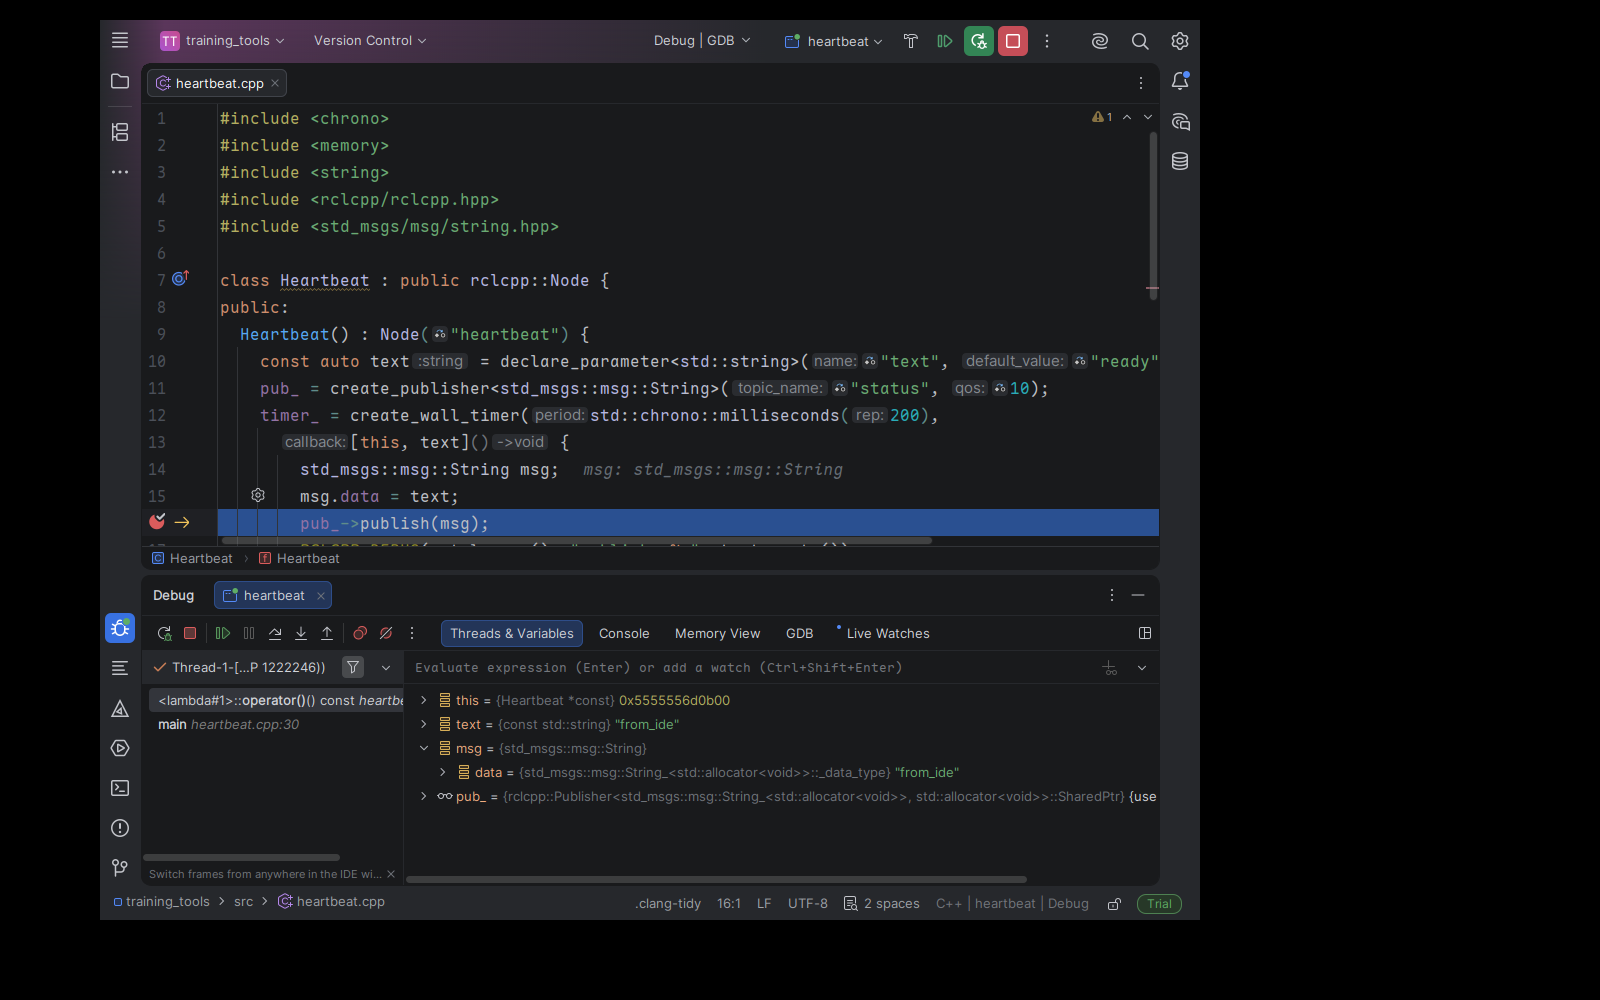
\includegraphics[width=0.9\textwidth,trim=100bp 180bp 400bp 300bp,clip]{images/ros2_clion_revised.png}
\caption{真实 CLion 调试窗口：发布回调暂停，消息文本已由运行参数覆盖}
\label{fig:ros2-clion-callback}
\end{figure}
\end{example}

CLion 的 Build 只负责所选构建目标。设置 \texttt{CMAKE\_INSTALL\_PREFIX} 仅改变安装目的地，不会自动执行安装。需要从 \texttt{ros2 run} 启动修改后的代码时，应由 colcon 重建并安装，或明确执行 IDE 的 install 目标；同时确认运行时加载的是该安装前缀。调试 IDE 构建目录中的目标时，则直接使用该目标。

\subsubsection{CLion：用编译数据库浏览多包工程}
编译数据库（compilation database）记录每个翻译单元实际使用的编译器、宏和头文件搜索路径，适合让 IDE 按 colcon 的真实参数索引代码。

\begin{example}[生成并核对索引来源]
\par\medskip\noindent\begin{minipage}{\linewidth}
\begin{tbash}
cd ~/ros2_ws
colcon build --packages-select training_tools --cmake-args -DCMAKE_EXPORT_COMPILE_COMMANDS=ON
test -f build/training_tools/compile_commands.json
\end{tbash}
\end{minipage}\par\smallskip
在 CLion 的 File $\rightarrow$ Open 中选择这个 JSON，再选 Open as Project，以编译数据库项目打开，核对 heartbeat.cpp 的包含路径。你可以在 \texttt{rclcpp/rclcpp.hpp} 上跳转到实际头文件，确认它来自当前发行版的安装目录。它只涵盖该包；修改项目根目录不会自动合并其他包的编译数据库。接口包须先构建，生成的消息头文件才存在。需要整个工作空间索引时，应显式收集各包的数据库并按工具支持方式合并。
\end{example}

\Needspace{18\baselineskip}
\subsubsection{CLion：排查库头文件的解析参数}
这时候你可能会碰到一个看起来很矛盾的情况：heartbeat.cpp 能编译，跳进 rclcpp.hpp 却满屏红线，提示它自己的子头文件找不到。先别急着重装 ROS，我们要检查的是编辑器解析这个文件时用了哪些参数。头文件通常没有独立的编译记录，编辑器需要借用包含它的源码的参数；如果这一步没有借到，只有系统头文件路径，就会找不到 ROS 的头文件。比较源码与外部头文件的 clangd 解析命令，确认缺少了哪些 include 路径。成功编译说明编译器的配置可用，不能顺便证明编辑器的配置也正确。

\begin{example}[给指定头文件补上当前源码的解析参数]
仅当你确认遇到了上面的参数缺失时再做这个例子。我们继续用同一个 training\_tools 工程，随书 \nolinkurl{examples/ros2/header_flags.py} 读取其编译数据库，输出一段 clangd 配置；它不执行编译命令，也不修改数据库。先把这个文件复制到 \texttt{\textasciitilde/ros2\_ws}，代码如下：
\Needspace{25\baselineskip}
\par\medskip\noindent\begin{minipage}{\linewidth}
\lstinputlisting[frame=single,basicstyle=\ttfamily\footnotesize,language=Python,numbers=left,firstline=1,lastline=22,caption={读取选定源码的编译命令}]{examples/ros2/header_flags.py}
\end{minipage}\par\smallskip
源码路径必须唯一对应一条命令，否则脚本会提示你核对路径或选对数据库。接下来只提取 include 路径、宏和语言标准，把相对 include 路径按原构建目录转成绝对路径；输出参数 \texttt{-o} 等构建选项没有复制过去。
\Needspace{26\baselineskip}
\par\medskip\noindent\begin{minipage}{\linewidth}
\lstinputlisting[frame=single,basicstyle=\ttfamily\footnotesize,language=Python,numbers=left,firstline=23,lastline=45,firstnumber=23,caption={生成只作用于指定头文件的配置}]{examples/ros2/header_flags.py}
\end{minipage}\par\smallskip
通用形式为 \texttt{python3 header\_flags.py 数据库 源码 头文件 [更多头文件]}。它输出 JSON，JSON 也是合法的 YAML。\texttt{If.PathMatch} 使用完整路径的正则表达式匹配，\texttt{re.escape} 把文件名中的点等字符转义，因此这段配置只作用于你选定的文件。先生成并查看片段：
\par\medskip\noindent\begin{minipage}{\linewidth}
\begin{tbash}
cd ~/ros2_ws
header=/opt/ros/$ROS_DISTRO/include/rclcpp/rclcpp/rclcpp.hpp
test -f "$header"
python3 header_flags.py build/training_tools/compile_commands.json \
  src/training_tools/src/heartbeat.cpp "$header" \
  > /tmp/ros-header-flags.json
cat /tmp/ros-header-flags.json
\end{tbash}
\end{minipage}\par\smallskip
这里的数据库和源码换成你的实际路径；头文件也以刚才跳转显示的路径为准。安装目录层级可能随软件包版本变化，先用 \texttt{test -f} 确认文件存在。确认输出与数据库中的 include 路径相符后，放进用户配置目录。已有配置先备份，再追加为一个新片段：
\par\medskip\noindent\begin{minipage}{\linewidth}
\begin{tbash}
cfg_dir="${XDG_CONFIG_HOME:-$HOME/.config}/clangd"
mkdir -p "$cfg_dir"
if [ -f "$cfg_dir/config.yaml" ]; then
  backup=$(mktemp "$cfg_dir/config.yaml.before-header-flags.XXXXXX")
  cp -p "$cfg_dir/config.yaml" "$backup"
  printf '备份：%s\n' "$backup"
  printf '\n---\n' >> "$cfg_dir/config.yaml"
fi
cat /tmp/ros-header-flags.json >> "$cfg_dir/config.yaml"
\end{tbash}
\end{minipage}\par\smallskip
配置放在这里，是因为库头文件位于工作空间之外，工作空间中的 \texttt{.clangd} 不会作用于它。IDE 需要使用同一个 \texttt{XDG\_CONFIG\_HOME}，默认不用额外设置；如果你用临时配置启动 IDE，就在那套临时目录里操作。随后关闭这个头文件标签，再从源码重新跳转，查看 Problems 中的诊断和实际解析参数。应能看到缺少的路径被补上，相应的找不到子头文件错误消失；保留诊断，并比较停用、恢复片段后的结果。

这只是把选定源码的解析条件借给选定头文件。其他包可能有不同的宏和路径，你要选它实际使用的源码重新生成；同一个头文件有多个编译上下文时也要先选定上下文。数据库、依赖或发行版变化后重新核对片段，不要把旧路径永久挂着。若仍有其他诊断，按其具体原因继续检查，不能一股脑关掉红线。
\end{example}

\begin{note}
可以从 Find Action 搜索 Show Clangd Tool Window 查看诊断工具；需要解析命令时，搜索 Registry，把 \texttt{clion.clang.clangd.debug} 临时设为 2，关闭并重开头文件后在 IDE 日志中查看 ASTWorker 的 command，查完恢复为 0。据此比较源码与头文件的实际 include 路径。配置格式和头文件参数借用机制分别见 \href{https://clangd.llvm.org/config}{clangd 配置文档}与 \href{https://clangd.llvm.org/design/compile-commands}{编译命令说明}；不要把 clangd 进程自身的参数与它解析某个文件的编译参数混在一起。
\end{note}

\begin{exercise}
\label{ex:v2-ros-header-context}
从 heartbeat.cpp 的数据库条目中找出 rclcpp 的 include 路径，说明它与 \texttt{rclcpp/rclcpp.hpp} 拼接后怎样定位文件。生成只匹配该头文件的配置，核对路径与宏；把源码参数换成不存在的路径，确认脚本会拒绝输出。若你的 IDE 确实存在上述缺失参数的问题，再在保留诊断的前提下比较启用片段前后的结果；没有此问题时记录实际参数，不必人为制造红线。
\end{exercise}

\begin{conclusion}
\begin{itemize}
\item 找不到 ament：检查 IDE 环境；找不到生成接口头：先构建接口包。
\item CLion 与 colcon 使用不同构建目录，避免 CMake 缓存和生成器相互覆盖；两者不必强制使用同一种生成器。
\item 断点不命中：检查 Debug 配置、正在运行的二进制路径，以及代码是否重新构建。
\item 源码能编译但外部头文件报错：比较二者实际解析参数；给指定头文件补参数后仍保留诊断，按具体错误继续查。
\item build、install、log、\texttt{.idea}、\texttt{cmake-build-*} 和生成的编译数据库通常不提交 Git；源码、清单和启动配置需要提交。
\end{itemize}
\end{conclusion}
\begin{exercise}
\label{ex:v2-ros-ide}
先停止上面的节点，清除运行配置中的 \texttt{-p text:=from\_ide} 等文本覆盖，再在 IDE 中把默认文本改为 \texttt{from\_debug} 并构建；依次从 IDE 和旧安装目录运行，每次观察后停止当前发布者，避免混在一起。解释为何可能看到不同文本，给出让 \texttt{ros2 run} 使用新代码的步骤。
\end{exercise}


\Needspace{18\baselineskip}
\section{大图像链路：中间件与内存}
\subsubsection{先给 1440\texorpdfstring{$\times$}{×}1080@250 Hz 算笔账}
\label{sec:ros2-image-budget}
前面用字符串把收发流程跑通了，接下来换成我们实际工作中会碰到的图像。相机最高可以达到 $1440\times1080@250\,\mathrm{Hz}$（宽 $\times$ 高），也就是每隔 4 ms 来一帧。这个数字说的是相机的工作上限；接到 ROS2 后，采集、转换、传输和识别能不能一直跟上，还得分开测。你大概也不希望相机拍得飞快，识别节点却在认真处理半秒前的装甲板。

先把图像看成一块内存。每帧像素数是 $1440\times1080=1\,555\,200$，紧密排列时，原始像素负载率为
\[
  B=\text{宽}\times\text{高}\times\text{每像素字节数}\times\text{帧率}.
\]
这里使用十进制单位：$1\,\mathrm{MB}=10^6\,\mathrm{B}$，$1\,\mathrm{GB}=10^9\,\mathrm{B}$。表\ref{tab:ros2-image-budget} 只算像素，不含消息头、DDS 分片、协议开销或行尾填充。实际 \texttt{Image} 要核对 \texttt{step}，像素数组大小通常按 \texttt{step}$\times$\texttt{height} 计算；相机输出的打包格式也要先确认。

\begin{table}[htbp]
\centering
\caption{1440×1080、250 Hz 的紧密排列图像预算}
\label{tab:ros2-image-budget}
\begin{tabular}{lrrr}
\toprule
格式 & 每帧 / MB & 每秒 / MB & 纯像素 / Gbit/s\\
\midrule
mono8 / Bayer8 & 1.5552 & 388.8 & 3.1104\\
mono16 & 3.1104 & 777.6 & 6.2208\\
bgr8 / rgb8 & 4.6656 & 1166.4 & 9.3312\\
\bottomrule
\end{tabular}
\end{table}

\begin{example}[复制一帧，到底搬了多少东西]
假设相机先输出 Bayer8，我们在采集端转成 BGR8，再把完整彩色图像交给识别节点。一秒的 BGR8 像素就有约 1.17 GB。每多做一次完整复制，都要读一遍源数据、写一遍目标数据，按这个负载估算，新增的读写量约为 $2\times1.1664=2.3328\,\mathrm{GB/s}$。如果连续几段处理都各自复制一次，这笔账会不断叠加。

这个估算帮助我们定位值得优化的边界，不能当作内存总线实测值：缓存命中、写分配、DMA 和库实现都会改变真实流量。Bayer 转 BGR 本身也是一次产生新数据的处理，不能靠 \texttt{std::move} 把它省掉。跨机器时，千兆网连 mono8 的纯像素都装不下；BGR8 接近万兆网的标称带宽，还没有给协议和其他数据留足空间。应先规划分辨率、帧率、ROI、图像格式与网络，再挑中间件。
\end{example}

\paragraph*{队列深度救不了长期超时}
250 Hz 的到帧间隔是 4 ms；单个串行处理阶段若每帧要 8 ms，理想上限也只有 125 Hz。加大 \texttt{KeepLast} 深度可以吸收短时抖动，却不能提高长期处理能力。深度 5 的一份 BGR8 历史，仅像素就约 23.33 MB；多端历史和工作缓冲还会继续占内存。在 250 Hz 输入下，深度 10 对应约 40 ms 的入队跨度，这不是延迟上界；发布端阻塞、其他队列和调度等待都可能再增加图像年龄。

对于需要及时瞄准的识别链路，我们通常先用小深度、易于丢弃旧帧的策略作起点，例如兼容的 \texttt{best\_effort} 加 \texttt{KeepLast(1)} 或较小深度，再按丢帧与延迟实测调整。离线录制如果要求完整保存，就要另算存储吞吐和可靠传输成本，必要时降帧率或独立部署。可靠传输解决的是交付语义，不能把处理器的工作速度翻倍。

\begin{exercise}
\label{ex:v2-ros-image-budget}
计算该相机 Bayer8 和 BGR8 的负载率。若 BGR8 链路新增两次完整复制，估算新增读写量；再判断每帧串行处理 8 ms 时，把队列从 5 改成 100 能否持续处理全部 250 Hz 输入。说明你会同时记录哪两个指标，避免只看话题频率。
\end{exercise}

\subsubsection{中间件怎么选：先比较同一条链路}
\label{sec:ros2-rmw-selection}
\texttt{rclcpp} 下面的 RMW 是中间件接口，并不是某一家 DDS 产品的名字。Humble 的常用起点是 Fast DDS（\nolinkurl{rmw_fastrtps_cpp}），我们也可以换成 Cyclone DDS（\nolinkurl{rmw_cyclonedds_cpp}），或者使用基于 Zenoh 的 \nolinkurl{rmw_zenoh_cpp}。发布与订阅的基本代码通常不用跟着改，但发现机制、传输路径、缓存与配置方法会变化。小字符串测试能确认通信成立，大图像测试才能暴露吞吐、分片与排队问题。

\begin{center}
\begin{tabular}{p{0.17\textwidth}p{0.35\textwidth}p{0.35\textwidth}}
\toprule
实现 & 接入与发现 & 图像路径与评估重点\\
\midrule
Fast DDS & Humble 默认 RMW；按需使用自己的 XML 配置 & 同步/异步发布影响调用线程；共享内存传输与 Data Sharing 分开核对，默认未启用后者\\
Cyclone DDS & 安装对应 RMW 后切换；配置使用 \nolinkurl{CYCLONEDDS_URI} & 使用自己的传输与线程配置；本章借出探测为 false，不能套用 Fast DDS 的调优变量\\
Zenoh & 安装 \nolinkurl{rmw_zenoh_cpp}；默认通过路由器协助发现 & 同机 peer 可直接交换数据；共享内存需单独配置，不能把“使用 Zenoh”当作“已经零拷贝”\\
共同口径 & 两端使用相同 RMW、消息、QoS 与部署布局 & 一起看实际发送频率、接收比例、延迟尾部与资源占用，保留配置与原始日志\\
\bottomrule
\end{tabular}
\end{center}

切换操作见前面的环境小节。这里进一步要求两端显式设置同一种 RMW，停止旧节点后重启；试验使用独立域，避免遗留订阅者混进来。DDS 实现之间存在互操作能力，但当前实验应先排除混用实现造成的变量。尤其不要一边换 RMW、一边改可靠性和图像尺寸，最后凭“好像快了”给某一家颁奖。

\begin{example}[安排一个可以解释结果的对照]
本节与后两节共用 \path{examples/ros2/image-path-demo}。它生成同样的图像，先固定帧数、尺寸、频率、\texttt{best\_effort} 和深度 5，然后对两种 RMW 分别运行三种布局：两个进程、同一进程关闭进程内通信、同一进程开启进程内通信。这样，前两项帮助观察中间件与进程边界，最后一项帮助观察所有权传递；完整构建和命令在下一节。

结果至少一起看发送实际频率、接收比例和 P95/P99 延迟。P95 表示约 95\% 的已收到样本不超过这个延迟；丢掉的样本不在延迟统计中，因此低延迟也可能伴随大量丢帧。再记录 CPU 时间和内存作为辅助信息。在真正的系统选型前，至少重复几轮，补测实际相机、算法、录制和网络。
\end{example}

Fast DDS 的 RMW 默认项、同步与异步发布、Data Sharing 配置可查 \href{https://github.com/ros2/rmw_fastrtps/blob/humble/README.md}{Humble 分支说明}；需要调整网卡、发现与报文时，再查 \href{https://github.com/ros2/rmw_cyclonedds/blob/humble/README.md}{Cyclone DDS 的 ROS2 接口说明}。这些资料帮助你找到对应配置，最终选择仍要落在自己的链路数据上。

\paragraph*{把 Zenoh 接到同一条图像链路}
Zenoh 不是另一家 DDS。\texttt{rmw\_zenoh\_cpp} 把 ROS2 的中间件接口接到 Zenoh，所以我们仍然编写熟悉的节点、消息和组件，下面的发现与传输方式却换了。默认配置先连接本机 Zenoh 路由器，由它协助节点发现彼此；同机 peer 会建立直接连接，不能把它理解成“每帧图像都要绕路由器一圈”。需要跨主机、无线链路或多机器人通信时，可以进一步配置路由与连接拓扑，但这些条件还要另测。

\begin{example}[让 Zenoh 运行已有组件]
先完成下一节的 \path{image_path_demo} 构建，再回到这里操作。第一个终端在 Ubuntu 22.04/Humble 中安装接口并启动路由器：
\par\medskip\noindent\begin{minipage}{\linewidth}
\begin{tbash}
source /opt/ros/humble/setup.bash
sudo apt update
sudo apt install ros-humble-rmw-zenoh-cpp
ros2 run rmw_zenoh_cpp rmw_zenohd
\end{tbash}
\end{minipage}\par\smallskip
保持这个终端运行。第二个终端加载同一个组件工程，把 RMW 改为 Zenoh：
\par\medskip\noindent\begin{minipage}{\linewidth}
\begin{tbash}
source /opt/ros/humble/setup.bash
cd ~/image_path_ws
source install/setup.bash
export ROS_DOMAIN_ID=87
export ROS_LOCALHOST_ONLY=1
export RMW_IMPLEMENTATION=rmw_zenoh_cpp
ros2 launch image_path_demo path.launch.py mode:=intra
\end{tbash}
\end{minipage}\par\smallskip
默认仍是 64×48、25 Hz、100 帧。等 \texttt{SOURCE\_DONE} 后，先在第二个终端按 Ctrl+C 保存统计，再停止第一个终端的路由器。检查完整接收、\texttt{bad\_frames=0} 和进程内地址记录；这次节点源码没有改变。需要查询图时，查询终端也要加载同一工程、域和 RMW；可使用 \texttt{ros2 component list --no-daemon}，避免旧 RMW 的后台缓存混入结果。

若收不到消息，先查路由器是否启动、默认 7447 端口是否被占用、两端 RMW 和域是否一致，以及是否遗留 \texttt{ZENOH\_CONFIG\_OVERRIDE} 或自定义配置文件。这里两端都用 Humble；看得到远端节点不等于跨发行版消息能交付。Zenoh RMW 也不会自动与 DDS 节点或 \texttt{zenoh-bridge-ros2dds} 互通，桥接需要单独核对协议与部署。

停止手动实验后，可以直接让记录器管理每轮路由器并跑三种布局：
\par\medskip\noindent\begin{minipage}{\linewidth}
\begin{tbash}
python3 src/image_path_demo/compare.py \
  --output /tmp/image-path-zenoh-small \
  --rmws rmw_zenoh_cpp
\end{tbash}
\end{minipage}\par\smallskip
记录器使用自己的本机 17447 端口，启动前检查占用，退出时只关闭自己启动的路由器与节点；换端口用 \texttt{--zenoh-port}。默认仍不启用 Zenoh 共享内存。路由器的 CPU/RSS 也计入这一轮资源记录，不能遗漏它，再声称整个部署更省资源。
\end{example}

Zenoh 的发现、路由与参数可查 \href{https://github.com/ros2/rmw_zenoh/blob/humble/README.md}{Humble 安装与配置说明}和\href{https://github.com/ros2/rmw_zenoh/blob/humble/docs/design.md}{RMW 设计说明}。先把相同节点跑通，再测试大图像与实际网络，不能凭协议名字判断哪一个更快。

\begin{exercise}
\label{ex:v2-ros-rmw-choice}
运行下一节的小图像对照，找出 Fast DDS、Cyclone DDS 与 Zenoh 在 \texttt{separate} 模式下的发送频率、接收比例与 P95。列出本轮保持相同的条件，并说明 Zenoh 的路由器在本次实验中负责什么、如何正常停止。若其中一项更好，说明还需补测什么，才能决定实际相机使用哪个实现。
\end{exercise}

\subsubsection{零拷贝与组件容器：先管好图像的所有权}
\label{sec:ros2-image-components}
\textbf{零拷贝（zero-copy）一定要说清楚省掉哪一段复制。}我们先追求“相机发布节点到识别订阅回调”这一段的进程内像素传递：把两个节点装进同一个进程，让 \texttt{rclcpp} 直接交接消息的所有权。相机 SDK 向消息填数据、颜色转换、校正和 CPU/GPU 传输仍需分别检查。这一段省了复制，不等于整条采集与推理链路都没有复制。

\begin{figure}[H]
\centering
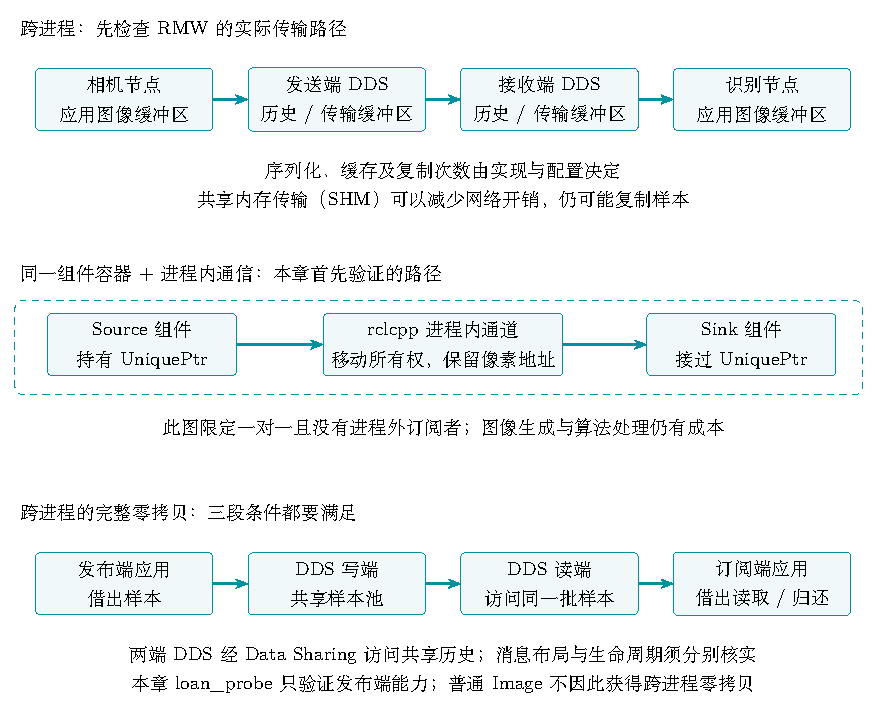
\includegraphics[width=0.97\textwidth]{images/ros2_image_paths_revised.pdf}
\caption{三种数据路径：区分进程内传递、共享内存传输与完整的跨进程零拷贝}
\label{fig:ros2-image-paths}
\end{figure}

图\ref{fig:ros2-image-paths} 中间一行是我们先动手验证的路径。\textbf{组件（component）}是可装载的节点实现，\textbf{组件容器（component container）}是承载它们的进程。组件不是一种新消息类型，也不会因为装到一起就自动启用进程内通信。两端要接收并使用 \texttt{NodeOptions}，启用 \nolinkurl{use_intra_process_comms}，并选择合适的消息所有权接口。

发布者创建 \texttt{UniquePtr}，通过 \texttt{publish(std::move(msg))} 交出消息，唯一订阅者用同类指针接过它。\texttt{std::move} 表达“可以转移所有权”，本身不保证任意传输路径零拷贝。实际能否直接交接，要看 \texttt{rclcpp} 的布局和订阅条件。交出以后不要继续访问原消息；接收端也不能留下一个裸指针，却让持有消息的智能指针先销毁。

\begin{note}
先前进入的 Distrobox、以及 Docker/Podman 的容器属于运行环境：它们管理文件系统、进程与设备等资源。ROS2 组件容器属于节点部署方式：它把组件放进同一个进程。两个节点即使在同一个 Distrobox 内，若分别启动两个进程，也仍不能使用这条 \texttt{rclcpp} 进程内路径。跨系统容器尝试 DDS 共享内存时，还要检查 IPC/共享目录、权限、容量与发现网络；网络能通不代表共享内存能用，GPU 驱动可用也不代表图像传输自动零拷贝。
\end{note}

\paragraph*{一份源码，三种部署}
\begin{example}[合成图像从 Source 交给 Sink]
先用默认的 $64\times48@25\,\mathrm{Hz}$ 跑通，再换成相机的大尺寸负载。项目不需要真实相机，接收端只检查首尾像素并统计回调入口时刻，暂时不做识别。目录如下：
\par\medskip\noindent\begin{minipage}{\linewidth}
\begin{tbash}
image-path-demo/
  package.xml             # 依赖与接口包声明
  CMakeLists.txt          # 消息生成、组件注册和安装
  msg/Frame.msg           # 图像与实验测量元数据
  src/components.cpp     # Source、Sink 两个组件
  src/loan_probe.cpp     # 下一节的借出能力探测
  launch/path.launch.py  # 相同节点的三种布局
  config/fastdds-loan.xml # 下一节的显式配置
  compare.py             # 独立进程组运行并保存统计
\end{tbash}
\end{minipage}\par\smallskip

\texttt{Frame.msg} 给正常的 \texttt{sensor\_msgs/Image} 加一层实验包装，序号、单调时钟和源缓冲区地址都放在包装里。\texttt{Image.header.stamp} 仍是节点时钟下的生成时间，\texttt{frame\_id} 仍表示相机坐标系，不拿它们偷偷塞测试字符串。
\par\medskip\noindent\begin{minipage}{\linewidth}
\lstinputlisting[frame=single,caption={图像包装接口}]{examples/ros2/image-path-demo/msg/Frame.msg}
\end{minipage}\par\smallskip

下面是完整的组件源码。Source 等订阅者出现后，按定时器周期分配并填充像素；完成指定帧数后停止发布。\texttt{sent\_ns} 在填充完成后、调用 publish 前记录，所以延迟统计从这里起算，发送频率则还会受到分配、填充与发送阻塞影响。
\lstinputlisting[frame=single,language=C++,caption={合成图像发布组件与公共定义},firstline=1,lastline=76]{examples/ros2/image-path-demo/src/components.cpp}

Sink 接到消息时记录延迟，检查首尾像素，再在正常退出时输出统计。地址只在源端与接收端 PID 相同、同一帧对应的情况下比较；跨进程的虚拟地址不能用于证明共享了物理内存。\texttt{work\_ms} 是可选的模拟处理耗时，默认 0。
\lstinputlisting[frame=single,language=C++,caption={图像接收组件与组件注册},firstline=77]{examples/ros2/image-path-demo/src/components.cpp}

本实验在同一台 Linux 上，用 \texttt{steady\_clock} 对应的单调时钟比较发送与回调入口时刻；不要直接把这个测法搬到两台未同步时钟的机器。统计也不包含曝光、SDK 采集、图像填充和识别完成时间。实车更关心从采样到结果、再到执行时的图像年龄，后续要继续埋点。

接下来是完整清单与构建规则。清单声明组件库和消息生成依赖；CMake 生成 \texttt{Frame}、链接类型支持，再注册两个组件类。代码末尾的注册宏与 CMake 中的注册函数配合，容器才能按插件名找到类。
\lstinputlisting[frame=single,language=XML,caption={组件实验依赖清单}]{examples/ros2/image-path-demo/package.xml}
\lstinputlisting[frame=single,language=cmake,caption={接口生成、组件注册与安装规则}]{examples/ros2/image-path-demo/CMakeLists.txt}

Launch 文件保持相同 Source/Sink 和 QoS，只改变布局。\texttt{separate} 启动两个组件容器进程；\texttt{same} 把两者装进同一进程但关闭进程内通信；\texttt{intra} 放到同一进程并为两端启用它。这里使用单线程 \texttt{component\_container}，避免线程并发把最小实验变复杂。
\lstinputlisting[frame=single,language=Python,caption={切换组件布局的 Launch 文件}]{examples/ros2/image-path-demo/launch/path.launch.py}

在 Ubuntu 22.04/Humble 环境内操作。下面把教材所在目录保存为 \texttt{BOOK}，替换成你的路径；工作空间使用新目录，已有同名包时换一个目录，避免覆盖。Bash 中的环境脚本按下面写，Zsh 则使用对应的 \texttt{setup.zsh}。
\par\medskip\noindent\begin{minipage}{\linewidth}
\begin{tbash}
source /opt/ros/humble/setup.bash
sudo apt install ros-humble-rmw-cyclonedds-cpp \
  ros-humble-rclcpp-components ros-humble-rosidl-default-generators
BOOK="$HOME/Apps/Tutorial4New"
mkdir -p ~/image_path_ws/src
cp -r "$BOOK/02-专项技术栈/examples/ros2/image-path-demo" \
  ~/image_path_ws/src/image_path_demo
cd ~/image_path_ws
rosdep install --from-paths src --ignore-src -r -y
colcon build --packages-select image_path_demo \
  --cmake-args -DCMAKE_BUILD_TYPE=Release
source install/setup.bash
export ROS_DOMAIN_ID=87
export ROS_LOCALHOST_ONLY=1
export RMW_IMPLEMENTATION=rmw_fastrtps_cpp
ros2 launch image_path_demo path.launch.py mode:=intra
\end{tbash}
\end{minipage}\par\smallskip
预期先出现三条 \texttt{POINTER} 输出，同一帧的 source 与 sink 像素地址相同，\texttt{same\_process=1}；约四秒后出现 \texttt{SOURCE\_DONE 100}。随后按 Ctrl+C 正常结束，查看 \texttt{SOURCE} 与 \texttt{SINK} 汇总：默认小输入应收到 100 帧、\texttt{bad\_frames=0}、\texttt{pointer\_matches=100}。逐帧打印会干扰高速实验，因此项目只打印前三帧及汇总。正常退出用于输出统计，直接强制杀死进程不会得到完整记录。

还可以在另一个加载相同环境、域和 RMW 的终端执行 \texttt{ros2 component list}，看到同一个 \texttt{/image\_box} 下有两个组件。若提示找不到类，核对两处注册名称、构建结果及工作空间环境；若组件存在但收不到消息，回到域、RMW、话题和 QoS 排查。只改 Launch 的 \texttt{mode:=same} 后重复运行，再改成 \texttt{mode:=separate}，应分别看到同进程的普通通信与两个不同 PID 的通信。\texttt{same} 的地址偶然复用不能证明零拷贝，判断必须结合实际启用选项与所有权路径。

切到小图像自动对照时，先停止手动实验，也停止额外的 echo、录制或显示订阅者。\texttt{compare.py} 会依次运行两种 RMW 与三种布局，给每次启动建立独立进程组，等发布完成并留出接收排空时间，再正常关闭这些进程。它清除所测进程里的 DDS 调优变量，不改你的启动文件。
\par\medskip\noindent\begin{minipage}{\linewidth}
\begin{tbash}
cd ~/image_path_ws
python3 src/image_path_demo/compare.py \
  --output /tmp/image-path-small
\end{tbash}
\end{minipage}\par\smallskip
输出目录必须尚不存在；再次运行时换一个名字。里面的 \texttt{results.json} 保存统计，各轮 \texttt{.log} 保留原始输出，\texttt{environment.json} 记录测量口径。参数的一般形式是 \texttt{--width 宽 --height 高 --channels 通道数 --rate 频率 --frames 帧数}；通道数本例只支持 1 与 3，分别对应 mono8 与 bgr8。\texttt{--repeat} 指定重复次数，\texttt{--modes} 可只选择一种布局，\texttt{--domain} 应选一个没有其他实验占用的域。
\end{example}

\paragraph*{系统容器部署：运行环境和共享资源一起检查}
Ubuntu 22.04 的 Distrobox 让我们在同一台主机上保持 Humble 的依赖环境；NVIDIA 支持则把匹配宿主驱动的用户态库与设备接进来。主机负责内核驱动，不要为了容器里的 ROS2 再装一套不匹配的内核驱动。组件容器可以运行在这个环境内，二者是可以同时使用的部署层次。

\begin{example}[进入环境后先确认资源边界]
下面第一条在宿主终端执行，后面的命令在容器内执行。已有 \texttt{ubuntu2204} 环境时直接进入；名称不同时换成自己的。普通 Ubuntu 教学机可以直接检查后面的环境与资源。
\par\medskip\noindent\begin{minipage}{\linewidth}
\begin{tbash}
distrobox enter ubuntu2204
echo "$ROS_DISTRO"
df -h /dev/shm
ls -l /dev/nvidia0 /dev/nvidiactl
nvidia-smi
\end{tbash}
\end{minipage}\par\smallskip
环境加载后应是 humble；为空时先加载适合当前 Shell 的环境脚本。\texttt{df} 检查共享内存挂载的可用容量，设备与 nvidia-smi 检查 NVIDIA 设备/驱动是否可见；没有 NVIDIA 时跳过后两条，按你的 GPU 平台检查。设备可见不代表本例用上了 GPU，本例是 CPU 图像通信测试。

系统容器的网络、IPC 模式和共享目录还需从实际部署配置核对。当前教学 Distrobox 共享宿主网络与 IPC，共享内存挂载约 32 GiB；其他 Podman/Docker 容器可能有独立命名空间与较小容量，不能照抄这个结果。BGR8 的几 MB 样本再乘历史深度、端点和工作缓冲，可能很快超出默认资源预算。遇到共享内存分配失败或传输回退时，先确认路径、权限、容量和实现配置；发现不通则先查域与网络。跨系统容器的完整共享样本交付须另行验证。
\end{example}

\paragraph*{组件化省下复制，也改变故障边界}
同一个进程里的相机、预处理与识别组件共享故障命运：其中一个崩溃，整个容器可能一起退出。单线程执行器中，一个耗时回调还会推迟其他回调。改用多线程容器 \nolinkurl{component_container_mt} 时，也要安排回调组（callback group）并检查共享数据；多线程既不自动保证并行，也不自动解决竞争条件。

因此，你可以先把需要传大图像的近邻节点组合起来，把控制、监控等职责按故障隔离要求拆开。多个订阅者也要考虑所有权：一份消息不能同时独占地交给两个 \texttt{UniquePtr} 接收者，可能产生复制；只读共享则要明确生命周期。外部录制、可视化或网络订阅者加入后，还可能触发额外的中间件发送。实验里暂时不加它们，部署时再逐个补测。

使用 OpenCV 时，\texttt{cv::Mat} 可以视图方式引用已有像素，也可能通过 \texttt{clone}、颜色转换等操作新建数据；要逐处核对。进程内消息直接交接之后又立刻 clone，一样会把大图像再搬一遍。CPU 图像交给 GPU 推理的边界也单独检查，不能把“机器有显卡”算成零拷贝证据。

\begin{exercise}
\label{ex:v2-ros-components}
用同一份源码依次运行 \texttt{intra}、\texttt{same}、\texttt{separate}，记录组件容器、PID 是否相同和前三帧的地址。解释为什么只有开启进程内路径并转移所有权的条件与地址记录一起，才能支持本例的像素传递结论。再检查运行环境的共享内存与 GPU 设备可见性，说明同一个 Distrobox 内启动两个独立节点是否满足进程内通信条件，以及哪些 GPU 传输边界还没被本例验证。
\end{exercise}

\subsubsection{借出消息：向中间件借一块内存}
\label{sec:ros2-loaned-messages}
前面由应用创建消息，再在进程内转移所有权。\textbf{借出消息（loaned message）}换了一个内存来源：发布者向中间件借样本缓冲区，把内容直接写进去，发布后交还控制权。如果支持条件满足，就能减少应用与中间件之间的一次复制或分配。它与组件化相关，却不是同一个开关，也不要求节点一定在同一个进程。

这里最容易踩坑的是 \texttt{borrow\_loaned\_message()} 的回退行为。底层不支持时，\texttt{rclcpp} 可以使用本地分配器继续运行；“借到了一个 C++ 对象”不能证明对象来自中间件。要先查询这个发布者的 \texttt{can\_loan\_messages()}，再记录实际 RMW、类型与配置。

\begin{example}[用 Float64 和 Image 探测借出能力]
沿用刚才的工程，完整程序如下。\texttt{Float64} 是简单固定大小类型；普通 \texttt{Image} 内含可变长像素数组与字符串。探测程序同时查询两者，再借出并发布一个值为 42 的 Float64。它只验证发布端借出和发布调用，不把订阅端或跨进程零拷贝算作已经验证。
\par\medskip\noindent\begin{minipage}{\linewidth}
\lstinputlisting[frame=single,language=C++,caption={借出能力与本地分配回退探测}]{examples/ros2/image-path-demo/src/loan_probe.cpp}
\end{minipage}\par\smallskip

在本章的 Humble/Fast DDS 实现中，固定类型还需要启用 Data Sharing，不能照搬“默认就能借出”的结论。项目给出一份显式配置，设置同步发布、可扩展的预分配历史，以及两端 Data Sharing 自动选择；它不强迫不支持的图像类型使用共享样本。
\par\medskip\noindent\begin{minipage}{\linewidth}
\lstinputlisting[frame=single,language=XML,caption={借出探测用的 Fast DDS 配置}]{examples/ros2/image-path-demo/config/fastdds-loan.xml}
\end{minipage}\par\smallskip

先从没有遗留 DDS 配置的终端开始，确认当前工作目录没有 \nolinkurl{DEFAULT_FASTRTPS_PROFILES.xml}，加载环境后依次运行。变量仅写在一条命令前，只影响那次进程；路径通过已安装包获取。
\par\medskip\noindent\begin{minipage}{\linewidth}
\begin{tbash}
source /opt/ros/humble/setup.bash
cd ~/image_path_ws
source install/setup.bash
export ROS_DOMAIN_ID=88
export ROS_LOCALHOST_ONLY=1
unset ROS_DISABLE_LOANED_MESSAGES
unset FASTRTPS_DEFAULT_PROFILES_FILE RMW_FASTRTPS_USE_QOS_FROM_XML
RMW_IMPLEMENTATION=rmw_fastrtps_cpp \
  ros2 run image_path_demo loan_probe
PROFILE="$(ros2 pkg prefix --share image_path_demo)/config/fastdds-loan.xml"
RMW_IMPLEMENTATION=rmw_fastrtps_cpp \
  FASTRTPS_DEFAULT_PROFILES_FILE="$PROFILE" \
  RMW_FASTRTPS_USE_QOS_FROM_XML=1 \
  ros2 run image_path_demo loan_probe
RMW_IMPLEMENTATION=rmw_cyclonedds_cpp \
  ros2 run image_path_demo loan_probe
RMW_IMPLEMENTATION=rmw_fastrtps_cpp \
  FASTRTPS_DEFAULT_PROFILES_FILE="$PROFILE" \
  RMW_FASTRTPS_USE_QOS_FROM_XML=1 ROS_DISABLE_LOANED_MESSAGES=1 \
  ros2 run image_path_demo loan_probe
\end{tbash}
\end{minipage}\par\smallskip
本章验证环境下，四轮 \texttt{LOAN} 输出的 \texttt{float64/image} 分别为 $0/0$、$1/0$、$0/0$、$0/0$。返回 0 的轮次会提示使用本地分配器；这是可用的回退路径。若你的结果不同，先记录版本与配置，再核对所用实现，不能为了让结果“像教材”而把 true 写死。
\end{example}

\paragraph*{Zenoh 的共享内存与借出 API 分开看}
Zenoh 同样能优化本机序列化数据的传输。项目记录器的 \texttt{--zenoh-shm} 会为节点与路由器显式启用共享内存及传输优化；本章使用的默认配置关闭这一功能。它可以在普通发布路径下工作，不要求应用先调用借出 API。本章 Zenoh 0.1.9 的 Float64/Image 探测在关闭和开启共享内存时均为 0/0，发布调用通过本地分配器回退完成。因此，\texttt{can\_loan\_messages()} 为 false 与“传输层可以使用共享内存”并不矛盾；普通 Image 仍有对象分配、填充及序列化/反序列化边界，不能把传输优化说成相机到算法的完整零拷贝。

先按第\ref{sec:ros2-rmw-selection}节启动自己的 Zenoh 路由器。在已加载 Humble 和组件工程的第二个终端运行发布端探测：
\par\medskip\noindent\begin{minipage}{\linewidth}
\begin{tbash}
RMW_IMPLEMENTATION=rmw_zenoh_cpp \
  ros2 run image_path_demo loan_probe
ZENOH_CONFIG_OVERRIDE='transport/shared_memory/enabled=true' \
  RMW_IMPLEMENTATION=rmw_zenoh_cpp \
  ros2 run image_path_demo loan_probe
\end{tbash}
\end{minipage}\par\smallskip
这里只有一个发布者，测的是借出接口，没有建立订阅端共享样本实验；不能拿这两次调用验证共享内存交付。结束后正常停止自己的路由器。

\begin{example}[开了共享内存，也要检查有没有回退]
在同一个工程里，先看容量与进程资源限制：
\begin{tbash}
df -h /dev/shm
ulimit -l
\end{tbash}
本轮容器的共享内存空间约 32 GiB，锁定内存上限却只有 8192 KiB，即 8 MiB。所用 Zenoh 会锁定共享段，默认 48 MiB 池超过这个限制，日志出现 \texttt{Error creating lazy ShmProvider} 与 \texttt{OS error 12}；消息仍能交付，所以“收到 1000 帧”不能证明共享路径生效。不要只看到 \texttt{enabled=true} 就宣布优化成功。

本实验改用 6 MiB 池重测，完整参数见第\ref{sec:ros2-image-measurement}节。这个设置足够放下一帧约 4.67 MB 的 BGR8，但可容纳的在途大样本很少；它是当前环境的演示条件，实际系统仍需按并发量规划池容量与资源限制。不要照搬 6 MiB 到所有相机。日志还要检查分配失败与回退；共享池创建成功也不能证明整条链路完全没有复制。
\end{example}

\paragraph*{为什么普通 Image 不能直接套用这个结论}
固定长度、可直接映射的 plain 消息布局适合共享样本池；字符串与可变长数组通常不能直接放到这种借出路径里。即使给序列规定一个最大长度，也不等于自动满足 plain 布局。\texttt{Image} 在上面的探测中返回 false，包装了它的 \texttt{Frame} 也不能靠外面多加几个字段就变成固定布局。

真要做跨进程大图像借出，需要设计并验证合适的固定布局或专门传输层，处理内存池容量、分辨率变化、两端生命周期与工具兼容性，还要核对生成的类型支持；不能随手把几 MB 的大数组放在栈上就宣称完成优化。对当前标准图像接口，先采用已验证的组件进程内路径，是更容易保持工具兼容与教学清晰的起点。

\paragraph*{共享内存传输不等于完整零拷贝}
共享内存传输（SHM transport）主要改变 DDS 的传输通道，样本仍可能复制到传输缓冲区再从中取出。Data Sharing 让读写端访问共享样本历史；若应用两端仍然复制到自己的对象里，也还没有消除整条路径的复制。图\ref{fig:ros2-image-paths} 最后一行需要发布端借出、共享样本交付和订阅端借出读取一起成立。

订阅端借出还涉及实现支持与样本有效期限制；本章不通过全局设置 \nolinkurl{ROS_DISABLE_LOANED_MESSAGES=0} 去强行开启它。普通订阅收到 42，最多证明这个值被交付，不能证明接收端从共享池直接借读。发布成功后，原借出对象已不归应用继续读写；没发布的借出对象也要按接口归还，\texttt{rclcpp::LoanedMessage} 的生命周期管理帮助你处理这一点。

这几项分别对应 \href{https://github.com/ros2/rclcpp/blob/humble/rclcpp/include/rclcpp/loaned_message.hpp}{Humble 的借出与回退实现}、\href{https://github.com/ros2/rmw_fastrtps/blob/humble/rmw_fastrtps_cpp/src/publisher.cpp}{发布者借出条件}，以及 \href{https://fast-dds.docs.eprosima.com/en/v2.6.11/fastdds/use_cases/zero_copy/zero_copy.html}{Fast DDS 的完整零拷贝条件}。查资料时分清 DDS 库具备的能力、RMW 暴露的能力和你的节点实际使用的路径。

\begin{exercise}
\label{ex:v2-ros-loans}
保存四轮 DDS loan\_probe 的原始输出，找出真正从中间件借出 Float64 的轮次；再比较 Zenoh 关闭与开启共享内存的借出输出。解释 Image 返回 false、程序却仍能运行的原因，以及为什么这份记录不能证明跨进程图像已经完整零拷贝。写出借出对象发布后必须遵守的所有权规则。
\end{exercise}

\begin{conclusion}
\begin{itemize}
\item RMW 选择决定通信实现，QoS 决定交付与历史策略；两者都不能补足不足的处理能力。
\item ROS2 组件容器安排节点的进程边界，Distrobox 安排运行环境；同进程还需启用进程内通信并管理所有权。
\item 进程内直接交接、DDS 共享内存传输、Data Sharing、Zenoh 传输优化与借出消息分别解决不同边界；零拷贝结论必须指出范围。
\item 借出 API 可以回退。先看能力、消息布局与配置，再看实际缓冲区和生命周期。
\end{itemize}
\end{conclusion}

\subsubsection{把负载升到 250 Hz，再看图像有没有变旧}
\label{sec:ros2-image-measurement}
现在小图像已跑通，我们把合成负载改成 $1440\times1080$ 的 BGR8。尺寸与目标频率来自前面的相机场景，像素由内存生成；这次测试没有接相机、转换 Bayer 或运行识别算法。目标 250 Hz 是定时器请求，不是程序预先保证的实测结果。

\begin{example}[重复三轮，保存吞吐与延迟记录]
先停止手动节点与额外订阅者，在同一个工作空间执行：
\par\medskip\noindent\begin{minipage}{\linewidth}
\begin{tbash}
python3 src/image_path_demo/compare.py \
  --output /tmp/image-path-bgr250 \
  --width 1440 --height 1080 --channels 3 \
  --rate 250 --frames 1000 --repeat 3
\end{tbash}
\end{minipage}\par\smallskip
每种组合正常发完 1000 帧后留两秒接收排空时间；程序输出实际发送/接收频率、接收比例与 P95。统计源码见 \texttt{compare.py}，参数和计时点已在环境记录中写明。出现未完成、缺少正常退出统计或像素检查失败时，脚本会报错并保留日志，不会把失败轮次填成零延迟。

% DDS: bgr250-1440x1080 的 18 轮；Zenoh: 本轮 bgr250 的 9 轮与 shm-6mib 的 3 轮。
\begin{table}[htbp]
\centering
\small
\caption{同机合成 BGR8 大图像对照，每项为三轮数值的中位数}
\label{tab:ros2-image-results}
\begin{tabular}{llrrrr}
\toprule
RMW & 布局 & 发送 / Hz & 接收 / Hz & 接收比例 & P95 / ms\\
\midrule
Fast DDS & separate & 250.0 & 87.5 & 34.7\% & 2.445\\
Fast DDS & same & 250.0 & 250.2 & 100.0\% & 0.968\\
Fast DDS & intra & 250.0 & 250.0 & 100.0\% & 0.042\\
Cyclone DDS & separate & 250.0 & 249.6 & 99.7\% & 3.580\\
Cyclone DDS & same & 250.1 & 250.2 & 100.0\% & 0.959\\
Cyclone DDS & intra & 250.0 & 250.0 & 100.0\% & 0.031\\
\midrule
Zenoh & separate & 250.1 & 250.3 & 100.0\% & 3.243\\
Zenoh & same & 250.0 & 250.2 & 100.0\% & 0.913\\
Zenoh & intra & 250.0 & 250.0 & 100.0\% & 0.029\\
Zenoh + SHM & separate & 250.0 & 250.4 & 100.0\% & 1.822\\
\bottomrule
\end{tabular}
\end{table}
这组 $1440\times1080$ 的 BGR8 数据在 2026 年 10 月 3 日的 Ubuntu 22.04/Humble Distrobox 中测得，主机为 i7-12700H，系统识别约 62.6 GiB 内存；Fast DDS 与 Cyclone DDS 的 RMW 分别为 6.2.10 与 1.3.5，Zenoh RMW/vendor 均为 0.1.9，Fast DDS 为 2.6.12，rclcpp 为 16.0.21。容器共享宿主网络和 IPC，测试清除 DDS/Zenoh 调优变量，深度 5、best\_effort、没有外部订阅者、没有算法工作。每轮发送 1000 帧，再留两秒排空；表中各项分别取中位数，P95 未跨轮合并样本。

Fast DDS 的 separate 接收比例三轮为 34.7\%、35.9\%、18.1\%；Cyclone DDS 为 99.7\%、99.7\%、99.8\%。在这个默认配置与输入下，后者交付比例更高；Fast DDS 已收到样本的 P95 较低，不能抵消丢掉的大量帧。两种 DDS 的 same 与 intra 共 12 轮都完整收到 1000 帧，intra 的像素地址记录全部匹配。

这些记录支持我们优先检查进程布局与所有权路径，也提醒我们继续核对配置，而不是给中间件排一个永久名次。

Zenoh 的三种布局各重复三轮，默认关闭共享内存，九轮均收到 1000 帧。它的路由器只监听本机独立端口，同机 peer 直接连接；本轮结果不能代替跨主机、无线或多机器人链路实测。表中最后一行是另外三轮显式配置：开启 Zenoh 共享内存并使用 6 MiB 池，不能与默认项混为一种配置。其 P95 中位数约 1.822 ms，默认 separate 约为 3.243 ms；进程内路径仍更短，说明传输优化与应用层所有权交接解决的边界不同。

最初用默认 48 MiB 池打开共享内存时，容器的 8 MiB 锁定内存限制导致分配失败。那三轮虽然也完整交付，却出现共享池错误，不能算作成功的 SHM 对照；回退记录另存，未放进上表。6 MiB 池的重测没有出现这个分配错误；后续仍要核对在途样本与回退，不能凭配置开关推断每帧路径或完整零拷贝。

小图像的 same 模式中，还出现过 50 帧里 49 次源/接收像素地址数值相等：它没有开启进程内通信，分配器复用地址造成了这种现象。因此，地址记录必须与启用选项、所有权和生命周期一起判断。

逐轮数据、原始日志与测量边界保存在仓库 \path{docs/revision/evidence/ros2-image-path-20261003-runtime/}。Zenoh 追加记录保存在 \path{docs/revision/evidence/ros2-zenoh-20261003-runtime/}。这些是合成像素通信数据，不是相机采集到识别完成的实测；CPU/GPU 转换与跨系统容器的共享样本路径也未由此验证。


观察时先问：Source 是否真的接近 250 Hz？如果没有，接收端频率低可能来自源端分配、发送阻塞或同进程回调争用；如果 Source 接近 250 Hz，接收比例却很低，才继续查交付与接收瓶颈。P95 低也要配合接收比例读，不能只拿已经收到的少数新帧做结论。\texttt{same} 与 \texttt{intra} 都有一个单线程容器，\texttt{separate} 有两个容器进程，所以对照同时体现部署布局的变化；不能把全部差值都算成某一种 DDS 内部复制的耗时。

记录器还保存本实验进程组的累计 CPU 秒和进程 RSS 之和。CPU 包括发现、加载与排空，不能直接当作稳态利用率；RSS 之和可能重复计算共享页，不能直接当作实际物理内存用量。真正选型时再分段测量、重复并改变实验顺序，必要时采用跟踪工具定位具体复制或等待位置。
\end{example}

\Needspace{9\baselineskip}
\paragraph*{把 Zenoh 加进大图像对照}
上面的默认命令保留两种 DDS。安装 Zenoh 后，保持相同图像、QoS 和三种布局，另用新目录运行：
\par\medskip\noindent\begin{minipage}{\linewidth}
\begin{tbash}
python3 src/image_path_demo/compare.py \
  --output /tmp/image-path-zenoh-bgr250 --rmws rmw_zenoh_cpp \
  --width 1440 --height 1080 --channels 3 \
  --rate 250 --frames 1000 --repeat 3
\end{tbash}
\end{minipage}\par\smallskip
需要一次调度三个实现时，用 \texttt{--rmws} 同时列出三种 RMW。记录器仍使用自己的路由器与本机端点，默认关闭 Zenoh 共享内存，避免把改变传输配置与改变 RMW 混成一个变量。

然后只保留两个进程，显式打开共享内存，并记录前面检查过的池容量：
\par\medskip\noindent\begin{minipage}{\linewidth}
\begin{tbash}
python3 src/image_path_demo/compare.py \
  --output /tmp/image-path-zenoh-shm \
  --rmws rmw_zenoh_cpp --modes separate --zenoh-shm \
  --zenoh-shm-pool-mib 6 \
  --width 1440 --height 1080 --channels 3 \
  --rate 250 --frames 1000 --repeat 3
\end{tbash}
\end{minipage}\par\smallskip
这是第二项独立对照，不能混入默认配置的结果。记录器保存共享内存开关、池容量、端口及路由器日志；检查 \texttt{zenoh\_shm\_provider\_error} 与原始日志，再读吞吐和延迟。资源限制、历史深度和在途样本都可能改变结果；即使本轮完整交付，也要继续测算法、实际相机与网络。

\paragraph*{故意让识别变慢一次}
接下来只保留 Fast DDS 的两个进程，把 Sink 的模拟处理设为 8 ms。先用默认小图像观察排队，不让图像大小掩盖处理能力问题：
\par\medskip\noindent\begin{minipage}{\linewidth}
\begin{tbash}
python3 src/image_path_demo/compare.py \
  --output /tmp/image-path-slow \
  --rmws rmw_fastrtps_cpp --modes separate \
  --rate 250 --frames 500 --work-ms 8 --depth 5
\end{tbash}
\end{minipage}\par\smallskip
预期接收处理跟不上到帧节奏，可能丢帧并出现等待；看实际发送频率、接收比例和延迟，不要求输出某个固定帧数。换用 \texttt{--depth 100}，对比丢帧与图像年龄。较深队列可能让更多旧帧被处理，代价是延迟；本例有限帧数可能最终排空，不能把“最后都收完”当作长期稳定。若慢处理需要更久排空，可增大 \texttt{--drain-seconds}，并把这个条件记录下来。

本次小图像实测中，两轮 Source 都接近 250 Hz，Sink 约为 122 Hz。深度 5 收到 249/500 帧，P95 约 20.0 ms；深度 100 收到 344/500 帧，P95 约 746.6 ms，两轮都使用两秒排空。较深的队列让这一轮收到了更多帧，也让已经收到的旧帧等得更久。数值是这次实验的结果，后续按自己的日志核对。

对串行的长期 8 ms 阶段，应该减少工作量、降采样、只处理最新帧，或设计可验证的并行流水线。零拷贝会减少搬运成本，却不能省掉算法本来需要的计算。图像容器还要配好外部观测边界：250 Hz 图像没必要全速送给 GUI，可以专门降频/缩小后输出给显示与录制节点。

\begin{exercise}
\label{ex:v2-ros-image-slow}
运行深度 5 和 100 的慢处理对照，记录实际发送频率、接收比例、P95 和排空时间。根据记录解释吞吐、丢帧和图像年龄的关系；再给相机到识别的主链路与降频可视化支路画一份部署方案，说明组件组合、进程隔离和 RMW 的选择依据。
\end{exercise}


\section{本章小结}
先用节点与话题划分职责，再用功能包管理代码和依赖。应熟练完成发布、订阅、定时器和自定义接口的最小闭环。工程运行按“声明依赖、构建安装、加载环境、Launch 启动、观察话题与日志”串联；发生问题时先检查实际使用的包和二进制路径，再检查域、发现范围、接口与 QoS。CLion 使用独立构建目录，运行环境应与终端一致。组件、安全通信和复杂 DDS 配置先会查对应发行版文档，再按项目需要展开。

\Needspace{12\baselineskip}
\begin{problemset}
\renewcommand{\theenumi}{\arabic{enumi}}
\item \label{prob:v2-ros-1}基础：一个包里有两个可执行程序，每个程序创建一个节点。包、进程、节点分别有几个？同一进程能否有多个节点？
\item \label{prob:v2-ros-2}基础：colcon build 后出现 build、install、log。运行前应加载哪个目录中的环境脚本？
\item \label{prob:v2-ros-3}基础：create\_publisher 的整数参数 10 是否表示“每秒发送十次”？哪个机制决定周期发布？
\item \label{prob:v2-ros-4}基础：包名 my\_msgs 与消息文件 My.msg 编译后，C++ 消息类型如何书写？
\item \label{prob:v2-ros-5}提高：发布者和订阅者使用相同话题名，仍收不到数据，按什么顺序排查？
\item \label{prob:v2-ros-6}实践：启动 demo\_nodes\_cpp 的服务端，调用 AddTwoInts，请求 a=-4、b=9，记录响应。
\item \label{prob:v2-ros-7}基础：修改所在发行版的本机发现范围设置后，为什么旧节点可能继续跨机器通信？它与 \nolinkurl{ROS_DOMAIN_ID} 是否能替代认证？
\item \label{prob:v2-ros-8}提高：Launch 中 namespace 为 blue、相对话题 status 重映射为 health，完整话题名是什么？源目录有 YAML，但启动时报文件不存在，应检查什么？
\item \label{prob:v2-ros-9}提高：定时器每 200 毫秒发布消息，INFO 日志按 2000 毫秒限流。两者频率分别是多少？FATAL 是否自动结束程序？
\item \label{prob:v2-ros-10}实践：同一包在 CLion 中运行的是新代码，ros2 run 却仍显示旧文本。说明构建、安装和环境三个环节的排查顺序，并给出修复命令。
\end{problemset}

\section{本章验收}
\begin{enumerate}
    \item 从空目录创建独立工作空间，现场运行字符串发布与订阅；由检查者更改输入文本，展示对应输出。
    \item 在完整工程中增加一个自定义字段并重新构建，展示接口查询、带时间戳的消息和定时器频率。
    \item 使用 rqt 或 Foxglove 展示数据流；关闭发布端再恢复，说明观察到的变化并提交构建命令。
    \item 提交包含清单、构建规则、参数与 Launch 的 training\_tools 包；由检查者指定命名空间和文本，现场启动并展示对应话题。
    \item 现场演示本机通信范围设置与恢复，保存一份独立实验日志；在 IDE 中命中发布回调断点，并说明实际运行的程序路径。
\end{enumerate}


% ============================================================
\chapter{多机通信方法}

\begin{introduction}
  \item 学习目标：实现 TCP 回环、拆帧与 ROS 桥接；验证 CRC、状态覆盖、事件重试和连接代次隔离。
  \item 建议学时：约 2--3 天。
  \item 本卷边界：本章使用教学帧，不替代裁判协议；赛场链路、真实字段及异常处置见卷三与队内接口文档。
\end{introduction}

\section{通信协议与故障处理}

\section{为何需要「多机通信」}

ROS2 话题适合同一机器人内多个节点协作。雷达站、反制机、电控裁判链路等场景里，进程往往分布在\textbf{不同机器或不同进程模型}上：
有的用 Python 独立进程，有的只提供 TCP/串口，并不暴露完整 ROS 图。
此时需要在话题之外掌握更底层的进程间 / 机间通信约定。

本章讨论三类常见手段：\textbf{本机 TCP}、\textbf{串口帧协议}、\textbf{可靠投递与故障隔离}。
赛场完整帧定义以当年裁判系统协议与队内仓库为准；此处讲模式与工程要点。

\section{通信拓扑与角色}

先分清谁听、谁连、谁拥有资源：

\begin{itemize}
    \item \textbf{Server / Client}：一方监听端口，另一方主动连接。雷达无线电侧常做 TCP Server，地面视觉做 Client 并自动重连。
    \item \textbf{唯一所有者}：同一物理设备（串口、SDR）同一时刻只应被一个进程打开；多进程抢占会导致错帧或设备占用失败。
    \item \textbf{单向与双向}：坐标/密钥可单向推送；控制指令（阵营、干扰等级）需反向通道。
\end{itemize}

示意：
\begin{tbash}
[无线电进程] --TCP 127.0.0.1:port--> [地面视觉进程] --串口--> [裁判系统]
[地面视觉] --另一串口--> [反制机进程]
\end{tbash}
本机环回地址避免把比赛数据接口裸露到局域网；跨机部署须另行考虑鉴权与防火墙。

\section{本机 TCP：粘包、拆包与最新值优先}

TCP 是字节流，没有「一帧消息」边界。接收端必须自行组帧：缓存字节，按协议切出完整帧，处理粘包（多帧连在一起）与拆包（一帧分多次到达）。

对雷达类高频状态，队列策略比「无限 FIFO」更重要：
\begin{itemize}
    \item \textbf{Latest-value}：同类命令只保留最新一条（如最新坐标、最新密钥），避免旧数据积压导致越发越旧。
    \item \textbf{优先级}：密钥、坐标通常高于次要状态信息。
    \item \textbf{连接代次（generation）}：每次新连接递增代数；旧连接线程禁止关闭或污染新 socket，防止重连竞态。
\end{itemize}

示意性伪代码：
\begin{tcode}
// 按 cmd_id 覆盖写槽位，而不是 push 到无界队列
void enqueue(uint16_t cmd, bytes payload) {
    slots[cmd] = payload; // 覆盖
}
bytes take_highest_priority() {
    for (cmd : priority_order)
        if (slots[cmd]) return pop(slots[cmd]);
    return {};
}
\end{tcode}

发送与接收均应校验连接代次；断开时清空待发槽与缓存，避免把上局数据发给新客户端。

\section{串口帧：定界、CRC 与重同步}

裁判系统、云台板、反制计数链路多用串口。典型二进制帧结构（示意，字段以官方协议为准）：
\begin{center}
\texttt{SOF | length | seq | CRC8 | cmd\_id | payload | CRC16}
\end{center}

工程要点：
\begin{itemize}
    \item 用 \texttt{/dev/serial/by-id/...} 固定设备路径，避免插拔后 \texttt{ttyUSB} 编号漂移；
    \item 波特率、校验位与对端严格一致；
    \item 坏 CRC 时丢弃并在字节流中重新搜索 SOF，实现\textbf{重同步}；
    \item 不同业务使用\textbf{独立物理串口}（裁判 / 云台 / 计数），避免一根线故障拖垮全站。
\end{itemize}

短控制包亦可更简，例如双字节定界 + 单字节命令（阵营、等级），同样需要粘包处理与非法字节跳过。

\section{与 ROS2 的关系}

\begin{itemize}
    \item 机内模块多、已有生态：优先 ROS2 话题 / 服务 / Action，配合 \texttt{qos}。
    \item 对接非 ROS 进程或嵌入式板：TCP/串口桥（Bridge）把外部帧转为内部消息，或反之。
    \item 调试：先单进程回环（模拟器发固定帧），再上实机；用 Wireshark / 串口抓包核对时序。
\end{itemize}

ROS2 的 DDS 发现与跨机组网是另一套问题（域名、防火墙、\texttt{ROS\_DOMAIN\_ID}）；雷达站常见部署是「同机多进程 + 串口出站」，与全场 ROS 多机发现不同。

\section{故障隔离清单}

| 故障 | 期望行为 |
|------|----------|
| 对端未启动 | 本端继续采集/解码；发送侧只保留最新槽 |
| TCP 断开 | 清空旧代次；Client 指数退避重连 |
| 串口拔出 | 打开失败可重试；其它链路不阻塞 |
| 数据过期 | 融合层丢弃陈旧源，回退次优源（见雷达融合） |

\section{练习建议}

\begin{enumerate}
    \item 实现一个本机 TCP echo：Client 重连后 Server 不混用旧连接。
    \item 解析带 SOF + 长度 + CRC 的字节流（可用假数据），覆盖粘包与半包。
    \item 为两类消息实现 latest-value 发送槽，并验证积压时始终发出最新坐标。
\end{enumerate}

延伸阅读：队内雷达开源架构说明（TCP / 裁判帧 / 多串口隔离），以及当年 RoboMaster 裁判系统通信协议文档。


\section{本章小结}
到这里，我们从一条字节流走到了完整消息：先分清角色和设备所有者，再按长度或帧头校验组帧，桥接时统一单位。状态使用有界最新值槽，事件使用确认、重试与去重；连接代次把每轮的数据和清理对应起来。应熟练复现半帧、粘包、坏 CRC、迟到清理和过期数据；真实协议、物理串口与跨机访问范围，按对应设备和当年文档继续核对。

\Needspace{12\baselineskip}
\begin{problemset}
\renewcommand{\theenumi}{\arabic{enumi}}
\item \label{prob:v2-comm-1}基础：同一设备字节流能否由两个互不协调的进程同时解析？建议如何组织读取和分发？
\item \label{prob:v2-comm-2}基础：服务端 bind、listen 后，客户端如何建立连接？随后服务端通过哪个对象收发？
\item \label{prob:v2-comm-3}提高：长度前缀为 3，却只收到两个载荷字节时连接关闭。能否把这半帧留给新连接补完？为什么？
\item \label{prob:v2-comm-4}基础：CRC 失败后为什么不能直接交付载荷？CRC 是否验证发送者身份？
\item \label{prob:v2-comm-5}基础：外部速度 3000 mm/s，内部接口使用 m/s，填多少？还需核对哪些时间与坐标约定？
\item \label{prob:v2-comm-6}提高：旧连接的清理回调在新连接建立后才到达。为什么“先检查代次，再不加锁地关闭当前 socket”仍可能有问题？
\item \label{prob:v2-comm-7}基础：同一位置槽写入 100、200、300 后消费一次，得到什么？若改为三次必须执行的购买事件，组织方法有何不同？
\item \label{prob:v2-comm-8}实践：运行 event\_demo，再模拟第一次确认丢失与所有确认丢失。分别记录实际执行数、发送次数和发送端结果；能否仅凭发送端失败断言业务没有执行？
\item \label{prob:v2-comm-9}提高：当前单调时钟为 12 秒，接收时间为 9 秒，最大年龄为 2 秒，应如何处理？能否直接拿远端未经同步的墙上时钟与本机单调时钟相减？
\end{problemset}

\section{本章验收}
\begin{enumerate}
\item 在两个终端运行 TCP 回显，按检查者指定端口断开并再次连接，展示新代次仍回显、旧清理被拒绝；说明每轮解析器归属。
\item 向解析器注入分片、噪声、坏 CRC 和有效恢复帧，展示只交付完整有效载荷；用 pySerial 伪终端复现读取和关闭异常，说明尚需实机检查的部分。
\item 暂停一条模拟链路，保持另一条继续消费；记录槽数、代次和过期计数。由检查者改过期阈值，解释结果变化。
\item 由检查者更改桥接距离，展示 ROS 话题中的米值；再演示确认丢失与有限重试，区分状态最新值和必须执行的事件。
\end{enumerate}


% ============================================================
\chapter{SDR 与电磁波解析}

\begin{introduction}
  \item 学习目标：录存并回放 IQ；实现教学 BPSK 的同步、解调和帧校验；演示配置切换与数据源时效检查。
  \item 建议学时：约 3--5 天。
  \item 本卷边界：仅训练离线接收与解析思路；本章示例不是当年赛场波形，实际频点和协议由队内文档确认，场景链路见卷三。
\end{introduction}

\section{接收链与离线解析}

\section{软件无线电在做什么}

\textbf{软件定义无线电（SDR, Software Defined Radio）}把本应由模拟电路固定的混频、滤波、解调等步骤，尽可能放到数字域用软件完成。
硬件负责射频前端与采样；主机或板载处理器对复数基带样本做同步、均衡、译码。

在 RoboMaster 雷达站场景中，SDR 常用于接收赛场规定的干扰波 / 信息波等波形，解出坐标、密钥等字段，再交给地面视觉融合与裁判上报。
\textbf{方向名「雷达」}指高台感知站；本章的射频硬件与导航章中的\textbf{激光雷达（LiDAR）}无关。

\section{从天线到 IQ}

简化接收链：
\begin{enumerate}
    \item 天线感应射频；
    \item 前端放大、滤波、下变频到中频或零中频；
    \item ADC 采样得到同相（I）与正交（Q）两路，合称 \textbf{IQ} 样本；
    \item 软件对 IQ 做数字滤波、相关、同步与帧解析。
\end{enumerate}

IQ 可看成复信号 $x = I + jQ$。采样率决定可观察的带宽量级；过高采样会受总线（如 USB）吞吐限制，需在带宽与丢样之间折中。

常用教学 / 开发板基于 Analog Devices 的 AD936x 系列收发器（如 ADALM-PLUTO 一类平台）。
主机侧常见软件栈：\textbf{libiio}（Industrial I/O）与 Python 封装 \textbf{pyadi-iio}，用于设置本振频率、采样率、增益，并读取 RX 缓冲。

示意（非赛场参数）：
\begin{tpython}
import adi
sdr = adi.ad9361(uri="ip:192.168.2.1")
sdr.sample_rate = 1_000_000
sdr.rx_lo = 2_400_000_000
iq = sdr.rx()  # complex 数组
\end{tpython}

实战中 URI、网段、天线与功率必须按队内部署文档配置；\textbf{任何发射}都须遵守当地频谱法规与比赛规则。

\section{波形、信道与「分阶段切换」}

赛场无线电往往不是单一载波一直不变，而是多种 profile（中心频、带宽、调制）分阶段出现，例如：
\begin{center}
干扰波一级 $\rightarrow$ 干扰波二级 $\rightarrow$ 信息波
\end{center}
同一块单通道 SDR 在任一时刻只盯一个 profile：确认上一级成功后再切换，避免「同时解两路」带来的复杂度与未验证风险。

工程上把每套射频参数做成 \textbf{radio profile}（本振、采样率、滤波系数等），由状态机驱动切换。
状态机输入可来自地面程序下发的阵营、干扰等级等控制字节。

\section{电磁波解析：从 IQ 到有效帧}

「解析」指从 IQ 流中恢复出协议定义的比特与字段。常见阶段：

\begin{enumerate}
    \item \textbf{前端数字处理}：直流消除、低通 / 匹配滤波、必要时抽取降速；
    \item \textbf{同步}：用已知前导或相关峰找到符号/帧起点（硬判决或软相关）；
    \item \textbf{解调与解映射}：按调制方式得到比特或软信息；
    \item \textbf{组帧与校验}：按长度切出候选帧，做 CRC；失败则滑动搜索下一候选；
    \item \textbf{字段解释}：命令字、坐标、密钥等进入上层（TCP / 融合模块）。
\end{enumerate}

\textbf{软判决}保留幅度/相关度量，而不是过早变成 0/1，往往在低信噪比下更稳。
对关键命令可做长度约束、字段边界搜索，减少盲目组合；CRC 失败的帧必须丢弃。

无硬件时，可用录制的 IQ 短样做离线回放，验证解码器回归——这是射频模块可复现测试的重要手段。

\section{与地面视觉的衔接}

解码成功的坐标帧（示意命令字如坐标上报）经本机 TCP 送给视觉进程后，融合层通常按\textbf{新鲜度}取舍：
无线电新数据优先；过期则回退视觉定位或其它兜底。
非坐标信息（血量、弹药、密钥等）可另槽转发，不阻塞坐标最新值。

通信层细节见本卷「多机通信方法」章；场地图定位与检测流水线见雷达方向其它专项与卷三。

\section{安全与合规*}

\begin{itemize}
    \item 开源或实验配置中的发射功率可能极低，\textbf{不等于}可以随意发射；须遵守法规与赛场管理。
    \item 不要在公开仓库提交真实比赛频点、大体积 IQ、含隐私的录包；用脱敏短样与哈希校验复现。
    \item 射频线缆、供电与接地不良会导致锁失、误码，排障时先分「射频前端 / 解码软件 / 上层通信」。
\end{itemize}

\section{练习建议}

\begin{enumerate}
    \item 用框图默写：天线 $\rightarrow$ IQ $\rightarrow$ 同步 $\rightarrow$ CRC $\rightarrow$ 上层消息。
    \item 说明为何单通道方案常用「分阶段切换」而不是同时解两路。
    \item 在无 SDR 条件下，对一段公开 IQ 样例跑通官方/队内离线解码脚本（若有），记录有效帧数。
\end{enumerate}

延伸阅读：Analog Devices Pluto / AD936x 用户文档；GNU Radio 与 libiio 入门；队内雷达开源中的无线电架构与射频安全说明。


\section{本章小结}
到这里，我们把“接收到了无线电数据”拆成了一条能逐步检查的链：硬件留下 IQ，数字处理找到参考并恢复比特，长度、CRC 和命令确认候选帧，字段再按单位、坐标系和时间进入上层。离线项目让你固定输入、修改参数、重放坏帧；它不能替代天线、调谐和真实波形的检查。先练熟录包、同步和拒收这几步，再按设备与协议文档补齐实际接收机。

\begin{problemset}
\renewcommand{\theenumi}{\arabic{enumi}}
\item\label{prob:v2-sdr-1} 基础：采样前已被模拟滤波器去掉的频段，能否在 IQ 回放时恢复？ADC 饱和又能否只换软件补好？
\item\label{prob:v2-sdr-2} 基础：IQ 为 $3+4j$，幅值是多少？若只保存幅值，正负频率与相位还剩下什么信息？
\item\label{prob:v2-sdr-3} 基础：采样率 8000 Hz、每符号 8 个样本，BPSK 的符号率与比特率分别是多少？本例一帧含前导但不含空样本，要几个样本？
\item\label{prob:v2-sdr-4} 提高：哈希一致但元数据的采样率写错，为什么回放仍可能错？给出比文件哈希更完整的录包交付约定。
\item\label{prob:v2-sdr-5} 基础：同步、符号判决和 CRC 分别解决什么？CRC 成功能否证明字段属于正确设备、坐标系和当前时刻？
\item\label{prob:v2-sdr-6} 提高：未知频偏与恒定相位有什么区别？为什么前导估计出的一个相角不能一直抵消频偏？
\item\label{prob:v2-sdr-7} 提高：切换到 information 后收到 level2 的迟到解码结果，应该检查什么？仅将状态名改过来是否已经完成实机切换？
\item\label{prob:v2-sdr-8} 基础：同一时钟下 now=20.0 s、radio=19.6 s、vision=19.9 s、有效期 0.25 s，选择哪一路？两路都过期或时间戳在未来时怎样处理？
\item\label{prob:v2-sdr-9} 实践：用 \texttt{--phase -1.2 --offset-hz -125 --x-mm 3000} 在新目录生成并回放；记录起点、字段、采样元数据，再故意损坏帧并展示拒收。写清它验证了哪些假设，尚未验证什么。
\end{problemset}

\section{本章验收}
\begin{enumerate}
\item 在两次独立进程中生成、保存、读取和解码录包；检查者更改相位、毫米坐标或合法频偏，能指出输入与结果的对应关系。
\item 对正常、CRC 损坏和截断样本分别演示处理结果，指出同步与帧校验的边界；不把理想单帧实验称为实战接收机。
\item 按检查者给出的事件序列展示配置阶段和代次，再模拟无线电过期、视觉可用及两路不可用，解释输出状态。
\item 记录已检查的硬件依赖与未验证项；有获准设备时现场接收一个缓冲、检查元数据并清理，说明真实波形解码所需的协议与同步条件。
\end{enumerate}


% ============================================================
\chapter{OpenCV 与图像处理基础}

\begin{introduction}
  \item 学习目标：构建图像工程；核对 Mat 与读写；实现分割、滤波、形态学与几何流水线；检查特征匹配和 ROS 图像接口。
  \item 建议学时：约 1--1.5 周。
  \item 本卷边界：聚焦 OpenCV 4.x 的基础接口；装甲板识别方案和赛场阈值调整见卷三。
\end{introduction}

\section{图像处理工具与流水线}

\subsubsection{OpenCV 简介与环境}

OpenCV（Open Source Computer Vision Library）是视觉组最常用的 C++ 图像处理库，
提供矩阵式图像表示、色彩空间转换、滤波、形态学、轮廓与特征等能力。
卷一 CMake 章已介绍 \texttt{find\_package(OpenCV REQUIRED)}，本节补齐安装与链接细节。

构建命令用于生成并执行编译规则，通用形式为 $cmake\enspace [OPTIONS]$。
\begin{center}
\begin{tabular}{lp{0.6\textwidth}}
\toprule[1.5pt]
参数 & 作用 \\
\midrule[1pt]
\texttt{-S PATH} & 指定源码目录 \\
\texttt{-B PATH} & 指定构建目录 \\
\texttt{--build PATH} & 构建已配置的目录 \\
\texttt{--target NAME} & 构建指定目标，与 --build 配合 \\
\texttt{-DNAME=VALUE} & 设置 CMake 缓存变量 \\
\bottomrule[1.5pt]
\end{tabular}
\end{center}
其余参数请查阅 cmake 帮助或 man 手册。

Ubuntu 22.04 上可通过 apt 安装开发包：
\begin{tbash}
sudo apt update
sudo apt install libopencv-dev
pkg-config --modversion opencv4
\end{tbash}

CMake 中推荐写法（OpenCV 4.x）：
\begin{tcode}
cmake_minimum_required(VERSION 3.16)
project(image_demo LANGUAGES CXX)
find_package(OpenCV REQUIRED)
message(STATUS "OpenCV: ${OpenCV_VERSION}")
add_executable(demo main.cpp)
target_include_directories(demo PRIVATE ${OpenCV_INCLUDE_DIRS})
target_link_libraries(demo PRIVATE ${OpenCV_LIBS})
\end{tcode}

常用头文件：\texttt{opencv2/opencv.hpp} 可一次引入核心模块；


仅处理图像时也可分别包含 \texttt{opencv2/core.hpp}、\texttt{imgproc.hpp}、\texttt{highgui.hpp}、\texttt{imgcodecs.hpp}、\texttt{videoio.hpp}。

\begin{example}
把本章任一完整 C++ 示例保存为 main.cpp，将上面的配置保存为 CMakeLists.txt。
先用下列程序确认链接成功：
\begin{tcode}
#include <opencv2/opencv.hpp>
#include <iostream>
#include <vector>
int main() {
    std::cout << CV_VERSION << "\n";
}
\end{tcode}
\end{example}

\begin{example}
构建命令通用形式为 $cmake\enspace [OPTIONS]$；-S 指定源码目录，-B 指定构建目录，--build 执行构建。其余选项查阅 cmake 帮助或 man 手册。本章固定使用独立构建目录。
\begin{tbash}
cmake -S . -B build
cmake --build build
./build/demo
\end{tbash}
\end{example}

\begin{exercise}
将目标名 demo 改为 image\_demo，重新配置、构建并运行。写出源码目录与构建目录分别在哪里。
\end{exercise}

\subsubsection{Mat：图像的核心数据结构}

\texttt{cv::Mat} 是 OpenCV 的核心类型，表示二维（或多维）数组。
彩色图通常为三通道 8 位无符号整数，类型记为 \texttt{CV\_8UC3}；灰度图为 \texttt{CV\_8UC1}。

\begin{itemize}
    \item \textbf{尺寸：}\texttt{rows}、\texttt{cols}、\texttt{channels()}、\texttt{size()}
    \item \textbf{类型：}\texttt{type()}、\texttt{depth()}（如 \texttt{CV\_8U}）
    \item \textbf{判空：}\texttt{empty()}，读图失败时必须检查
\end{itemize}

\textbf{浅拷贝与深拷贝。}
赋值与拷贝构造只复制表头，底层数据共享；修改一方会影响另一方。
需要独立副本时使用 \texttt{clone()} 或 \texttt{copyTo()}：
\begin{tcode}
cv::Mat A = cv::imread("input.jpg");
cv::Mat B = A;          // 共享数据
cv::Mat C = A.clone();  // 深拷贝
\end{tcode}

\textbf{像素访问。}BGR 三通道常用 \texttt{at}：
\begin{tcode}
cv::Vec3b px = img.at<cv::Vec3b>(y, x); // 注意顺序：行 y，列 x
uchar b = px[0], g = px[1], r = px[2];  // OpenCV 默认 BGR
\end{tcode}
性能敏感路径可用指针逐行扫描（\texttt{ptr<T>(row)}），避免对每个像素调用 \texttt{at}。

\textbf{ROI（Region of Interest，感兴趣区域）。}以下调用与原图共享内存：
\begin{tcode}
cv::Mat roi = img(cv::Rect(x, y, w, h));
\end{tcode}
若需独立处理，对 ROI 再 \texttt{clone()}。

\begin{example}
验证共享数据与独立副本。输出应为 9 1。
\begin{tcode}
#include <opencv2/opencv.hpp>
#include <iostream>
#include <vector>
int main() {
    cv::Mat a(2, 2, CV_8UC1, cv::Scalar(1));
    cv::Mat b = a, c = a.clone();
    b.at<uchar>(0, 0) = 9;
    std::cout << int(a.at<uchar>(0, 0)) << " "
              << int(c.at<uchar>(0, 0)) << "\n";
}
\end{tcode}
\end{example}

\begin{exercise}
将 b 改为 a 的单像素 ROI，重复修改。解释为什么 ROI 与 clone 的结果不同。
\end{exercise}

\begin{conclusion}
\begin{itemize}
\item Mat 表头保存尺寸和类型，数据可能被多个表头共享。
\item ROI 仍共享原图，clone 创建独立数据。
\item 访问像素先核对行列、通道和类型，再考虑性能。
\end{itemize}
\end{conclusion}

\subsubsection{图像与视频的读写}

\paragraph*{文件读写与窗口显示}
\begin{tcode}
#include <opencv2/opencv.hpp>
int main() {
    cv::Mat img = cv::imread("input.jpg", cv::IMREAD_COLOR);
    if (img.empty()) return -1;
    cv::namedWindow("demo", cv::WINDOW_AUTOSIZE);
    cv::imshow("demo", img);
    int key = cv::waitKey(0); // 0 表示一直等待按键
    if (key == 's') cv::imwrite("output.png", img);
    return 0;
}
\end{tcode}

\texttt{imread} 常用标志：\texttt{IMREAD\_COLOR}（默认 BGR 三通道）、
\texttt{IMREAD\_GRAYSCALE}、\texttt{IMREAD\_UNCHANGED}（保留 alpha 等）。
\texttt{imwrite} 根据扩展名选择编码格式。

\paragraph*{摄像头与视频流}
\begin{example}
设备就绪后运行以下完整程序，按 Esc 退出。保存为 main.cpp，使用本章首节构建配置。
\begin{tcode}
#include <opencv2/opencv.hpp>
int main() {
cv::VideoCapture cap(0); // 0 为默认摄像头；也可填视频路径
if (!cap.isOpened()) return -1;
cv::Mat frame;
while (true) {
    if (!cap.read(frame) || frame.empty()) break;
    cv::imshow("cam", frame);
    if (cv::waitKey(1) == 27) break; // Esc 退出
}
    return 0;
}
\end{tcode}
\end{example}

可用 \texttt{cap.set(cv::CAP\_PROP\_FRAME\_WIDTH, 1280)} 等属性尝试设定分辨率；
实际是否生效取决于驱动与设备。

\begin{example}
生成本地图像再读取，无摄像头也能检查文件路径。应输出 32 48。
\begin{tcode}
#include <opencv2/opencv.hpp>
#include <iostream>
#include <vector>
int main() {
    cv::Mat a(32, 48, CV_8UC3, cv::Scalar(0, 255, 0));
    if (!cv::imwrite("input.png", a)) return 1;
    cv::Mat b = cv::imread("input.png");
    if (b.empty()) return 2;
    std::cout << b.rows << " " << b.cols << "\n";
}
\end{tcode}
\end{example}

\begin{exercise}
把读取路径改为不存在的文件，确认程序返回 2；说明为何读图后必须先判空。
\end{exercise}

\subsubsection{色彩空间与颜色分割}

OpenCV 默认彩色图为 \textbf{BGR}，不是 RGB。灰度转换：
\begin{tcode}
cv::Mat gray;
cv::cvtColor(img, gray, cv::COLOR_BGR2GRAY);
\end{tcode}

识别任务中常转到 \textbf{HSV}：H 表示色调，S 饱和度，V 亮度。
在 8 位图上，OpenCV 的范围为 $H\in[0,179]$，$S,V\in[0,255]$
（与部分图像软件的 $H\in[0,360]$ 不同，换算时需注意）。

颜色分割用 \texttt{inRange} 生成二值掩膜，再用按位与提取前景：
\begin{tcode}
cv::Mat hsv, mask, result;
cv::cvtColor(img, hsv, cv::COLOR_BGR2HSV);
cv::inRange(hsv, cv::Scalar(100, 50, 50), cv::Scalar(130, 255, 255), mask); // 蓝示例
cv::bitwise_and(img, img, result, mask);
\end{tcode}

\textbf{红色的特殊处理。}红色落在色环两端附近，需两段区间再合并：
\begin{tcode}
cv::Mat m1, m2, mask;
cv::inRange(hsv, cv::Scalar(0, 70, 50), cv::Scalar(10, 255, 255), m1);
cv::inRange(hsv, cv::Scalar(170, 70, 50), cv::Scalar(179, 255, 255), m2);
mask = m1 | m2;
\end{tcode}
阈值需按光照与相机标定；可用取色工具或把单像素 BGR 转 HSV 后估计中心色相。

\begin{example}
直接构造色环两端的两个红色像素和一个蓝色像素，掩膜非零数应为 2。
\begin{tcode}
#include <opencv2/opencv.hpp>
#include <iostream>
#include <vector>
int main() {
    cv::Mat hsv(1, 3, CV_8UC3);
    hsv.at<cv::Vec3b>(0, 0) = {0, 255, 255};
    hsv.at<cv::Vec3b>(0, 1) = {179, 255, 255};
    hsv.at<cv::Vec3b>(0, 2) = {120, 255, 255};
    cv::Mat a, b, mask;
    cv::inRange(hsv, cv::Scalar(0,70,50), cv::Scalar(10,255,255), a);
    cv::inRange(hsv, cv::Scalar(170,70,50), cv::Scalar(179,255,255), b);
    cv::bitwise_or(a, b, mask);
    std::cout << cv::countNonZero(mask) << "\n";
}
\end{tcode}
\end{example}

\begin{exercise}
把第二个像素色调改为 90，预测并验证结果；再把第一个像素饱和度设为 0。
\end{exercise}

\subsubsection{阈值分割}

滤波与轮廓之前，常把灰度图转为二值图。

\textbf{固定阈值：}
\begin{tcode}
cv::Mat binary;
cv::threshold(gray, binary, 127, 255, cv::THRESH_BINARY);
\end{tcode}

\textbf{Otsu 自动阈值}（适合双峰直方图）：
\begin{tcode}
cv::threshold(gray, binary, 0, 255, cv::THRESH_BINARY | cv::THRESH_OTSU);
\end{tcode}

\textbf{自适应阈值}（光照不均时更稳）：
\begin{tcode}
cv::adaptiveThreshold(gray, binary, 255,
    cv::ADAPTIVE_THRESH_GAUSSIAN_C, cv::THRESH_BINARY, 11, 2);
\end{tcode}
其中块大小须为奇数；常数项用于微调局部阈值。

\begin{example}
用三像素灰度图检查固定阈值的边界，结果应为 0 0 255。
\begin{tcode}
#include <opencv2/opencv.hpp>
#include <iostream>
#include <vector>
int main() {
    cv::Mat gray = (cv::Mat_<uchar>(1,3) << 126,127,128);
    cv::Mat binary;
    cv::threshold(gray, binary, 127, 255, cv::THRESH_BINARY);
    for (int x=0; x<3; ++x) std::cout << int(binary.at<uchar>(0,x)) << " ";
    std::cout << "\n";
}
\end{tcode}
\end{example}

\begin{exercise}
改用 THRESH\_BINARY\_INV，先预测输出，再运行验证。
\end{exercise}

\subsubsection{滤波与降噪}

相机图像常含噪声。常见类型包括高斯噪声、椒盐噪声等。

\begin{figure}[H]
    \centering
    \begin{subfigure}{0.48\textwidth}
        \centering
        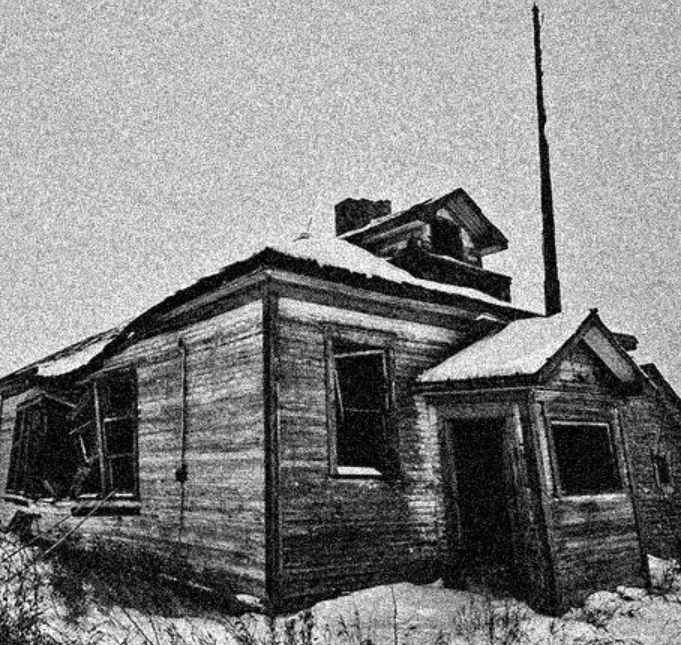
\includegraphics[width=\linewidth]{gaussian.png}
        \caption{高斯噪声}
    \end{subfigure}
    \hfill
    \begin{subfigure}{0.48\textwidth}
        \centering
        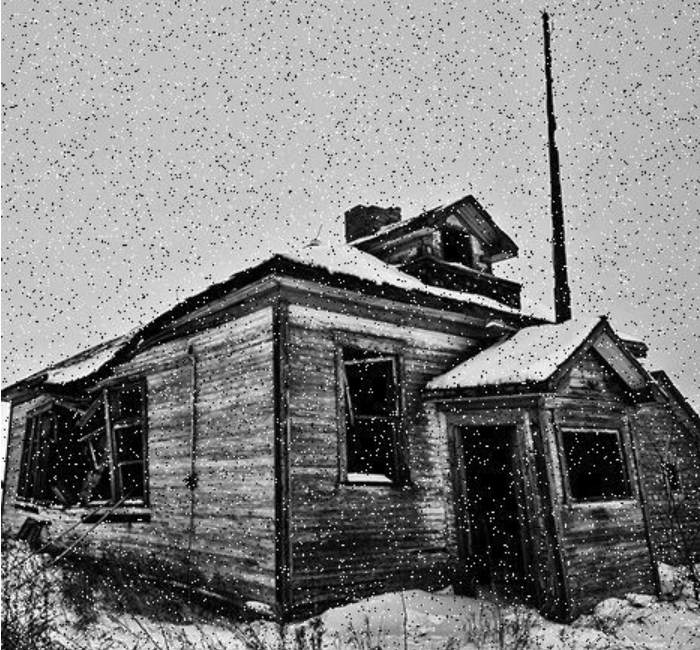
\includegraphics[width=\linewidth]{salt.png}
        \caption{椒盐噪声}
    \end{subfigure}
    \caption{常见图像噪声示例}
\label{fig:B_opencv-1}
\end{figure}

\begin{itemize}
    \item \texttt{cv::blur}：均值滤波，速度快，边缘易糊。
    \item \texttt{cv::GaussianBlur}：高斯加权，核宽高须为奇数；\texttt{$\sigma$} 可设为 $0$ 由核大小推断。
    \item \texttt{cv::medianBlur}：中值滤波，对椒盐噪声更有效。
    \item \texttt{cv::bilateralFilter}：双边滤波，平滑时尽量保边，计算更重。
\end{itemize}

\begin{tcode}
cv::Mat blurred;
cv::GaussianBlur(img, blurred, cv::Size(5, 5), 0);
cv::medianBlur(img, blurred, 5); // ksize 为奇数
\end{tcode}

边缘检测前通常先做轻度高斯模糊，以抑制噪声引起的伪边缘。

\begin{example}
用中值滤波去除孤立亮点，中心像素应从 255 变成 0。
\begin{tcode}
#include <opencv2/opencv.hpp>
#include <iostream>
#include <vector>
int main() {
    cv::Mat a = cv::Mat::zeros(7, 7, CV_8UC1), out;
    a.at<uchar>(3,3) = 255;
    cv::medianBlur(a, out, 3);
    std::cout << int(out.at<uchar>(3,3)) << "\n";
}
\end{tcode}
\end{example}

\begin{exercise}
改用 3×3 均值滤波，比较中心值；解释均值和中值为何不同。
\end{exercise}

\subsubsection{形态学操作}

形态学在二值图上用结构元素（核）做邻域运算，可去噪、填孔、连接断裂区域。

\begin{itemize}
    \item \textbf{腐蚀 \texttt{erode}}：缩小前景，去除毛刺。
    \item \textbf{膨胀 \texttt{dilate}}：扩大前景，弥合缝隙。
    \item \textbf{开运算}：先腐蚀后膨胀，去小噪点。
    \item \textbf{闭运算}：先膨胀后腐蚀，填小孔洞。
\end{itemize}

\begin{tcode}
cv::Mat kernel = cv::getStructuringElement(cv::MORPH_RECT, cv::Size(3, 3));
cv::Mat opened, closed;
cv::morphologyEx(binary, opened, cv::MORPH_OPEN, kernel);
cv::morphologyEx(binary, closed, cv::MORPH_CLOSE, kernel);
\end{tcode}

核形状可选 \texttt{MORPH\_RECT}、\texttt{MORPH\_ELLIPSE}、\texttt{MORPH\_CROSS}；
核越大，效果越强，也越容易抹掉细节。灯条等细长结构有时用椭圆核更合适。

\begin{example}
开运算去除孤立点，保留 5×5 方块。非零数应从 26 变成 25。
\begin{tcode}
#include <opencv2/opencv.hpp>
#include <iostream>
#include <vector>
int main() {
    cv::Mat a = cv::Mat::zeros(12,12,CV_8UC1), out;
    a(cv::Rect(4,4,5,5)).setTo(255);
    a.at<uchar>(1,1)=255;
    auto k=cv::getStructuringElement(cv::MORPH_RECT,cv::Size(3,3));
    cv::morphologyEx(a,out,cv::MORPH_OPEN,k);
    std::cout << cv::countNonZero(a) << " " << cv::countNonZero(out) << "\n";
}
\end{tcode}
\end{example}

\begin{exercise}
将核改为 7×7，检查方块能否保留。说明“大核去噪更强”的代价。
\end{exercise}

\begin{conclusion}
\begin{itemize}
\item 腐蚀缩前景，膨胀扩前景。
\item 开运算先腐蚀，闭运算先膨胀，二者顺序不可交换。
\item 核尺寸要与目标宽度比较；先保存中间图，再继续调参。
\end{itemize}
\end{conclusion}

\subsubsection{边缘检测与轮廓}

\paragraph*{Canny}
Canny 流程：高斯平滑 $\rightarrow$ 梯度 $\rightarrow$ 非极大值抑制 $\rightarrow$ 双阈值滞后。
两个阈值常用约 $1:2$ 或 $1:3$ 的比例：
\begin{tcode}
cv::Mat edges;
cv::Canny(gray, edges, 50, 150);
\end{tcode}

\paragraph*{轮廓提取与几何筛选}
\begin{tcode}
std::vector<std::vector<cv::Point>> contours;
std::vector<cv::Vec4i> hierarchy;
cv::findContours(edges, contours, hierarchy,
                 cv::RETR_EXTERNAL, cv::CHAIN_APPROX_SIMPLE);

for (const auto& c : contours) {
    double area = cv::contourArea(c);
    if (area < 100.0) continue; // 面积阈值按场景调整
    cv::RotatedRect rr = cv::minAreaRect(c);
    cv::Point2f pts[4];
    rr.points(pts);
    for (int i = 0; i < 4; ++i)
        cv::line(img, pts[i], pts[(i + 1) % 4], cv::Scalar(0, 255, 0), 2);
}
\end{tcode}

\begin{itemize}
    \item \texttt{RETR\_EXTERNAL}：只取最外层轮廓；\texttt{RETR\_TREE} 保留层级。
    \item \texttt{CHAIN\_APPROX\_SIMPLE}：压缩共线点，节省存储。
    \item 常用几何量：\texttt{contourArea}、\texttt{arcLength}、\texttt{boundingRect}、
          \texttt{minAreaRect}、\texttt{approxPolyDP}。
\end{itemize}

赛场上灯条、装甲板的具体面积比、长宽比与角度阈值见卷三；本卷先掌握工具。

\begin{example}
从实心矩形提取轮廓。应有 1 条外轮廓；连续几何面积为 171，非零像素为 200。
\begin{tcode}
#include <opencv2/opencv.hpp>
#include <iostream>
#include <vector>
int main() {
    cv::Mat a=cv::Mat::zeros(40,40,CV_8UC1);
    a(cv::Rect(5,5,20,10)).setTo(255);
    std::vector<std::vector<cv::Point>> cs;
    cv::findContours(a,cs,cv::RETR_EXTERNAL,cv::CHAIN_APPROX_SIMPLE);
    if(cs.size()!=1) return 1;
    std::cout << cs.size() << " " << cv::contourArea(cs[0]) << " "
              << cv::countNonZero(a) << "\n";
}
\end{tcode}
\end{example}

\begin{exercise}
对同一图运行 Canny 再提轮廓，比较数量与面积。说明像素数为何不总等于 contourArea。
\end{exercise}

\subsubsection{几何变换与绘图}

\textbf{缩放：}
\begin{tcode}
cv::Mat small;
cv::resize(img, small, cv::Size(), 0.5, 0.5, cv::INTER_AREA); // 缩小常用 AREA
\end{tcode}
放大可选用 \texttt{INTER\_LINEAR} 或 \texttt{INTER\_CUBIC}。

\textbf{旋转（绕中心）：}
\begin{tcode}
cv::Point2f center(img.cols / 2.0f, img.rows / 2.0f);
cv::Mat rotated;
cv::Mat M = cv::getRotationMatrix2D(center, 30.0, 1.0); // 角度、缩放
cv::warpAffine(img, rotated, M, img.size());
\end{tcode}

\textbf{常用绘图：}\texttt{line}、\texttt{rectangle}、\texttt{circle}、\texttt{putText}。
颜色仍按 BGR，例如绿色为 \texttt{Scalar(0,255,0)}。

\begin{example}
把 80×40 图像缩为一半，应得到 40×20；输出文件名为 small.png。
\begin{tcode}
#include <opencv2/opencv.hpp>
#include <iostream>
#include <vector>
int main() {
    cv::Mat a(40,80,CV_8UC3,cv::Scalar(0,0,0)), small;
    cv::circle(a,cv::Point(40,20),10,cv::Scalar(0,255,0),-1);
    cv::resize(a,small,cv::Size(),0.5,0.5,cv::INTER_AREA);
    if(!cv::imwrite("small.png",small)) return 1;
    std::cout << small.cols << " " << small.rows << "\n";
}
\end{tcode}
\end{example}

\begin{exercise}
按最近邻方式缩放，与 INTER\_AREA 比较圆边缘；说明插值选择与图像用途的关系。
\end{exercise}

\subsubsection{传统特征与匹配入门}

深度学习普及前，SIFT、ORB 等手工特征用于定位与匹配。
OpenCV 提供 \texttt{cv::ORB::create()}、\texttt{detectAndCompute} 与
\texttt{cv::BFMatcher} / \texttt{FlannBasedMatcher}。
视觉组日常识别以神经网络为主；在纹理稳定、算力受限或需要快速原型时，
ORB 仍可作为补充。深入匹配与位姿估计可结合相机标定与几何视觉章节。

\begin{example}
匹配相同图像的 ORB 描述子，匹配距离应全部为零；特征数量依版本略有差异。
\begin{tcode}
#include <opencv2/opencv.hpp>
#include <iostream>
#include <vector>
int main() {
    cv::Mat a(240,320,CV_8UC1);
    cv::RNG rng(42); rng.fill(a,cv::RNG::UNIFORM,0,256);
    auto orb=cv::ORB::create();
    std::vector<cv::KeyPoint> kp; cv::Mat desc;
    orb->detectAndCompute(a,cv::noArray(),kp,desc);
    if(desc.empty()) return 1;
    std::vector<cv::DMatch> matches;
    cv::BFMatcher(cv::NORM_HAMMING,true).match(desc,desc,matches);
    for(const auto& m:matches) if(m.distance!=0) return 2;
    std::cout << matches.size() << "\n";
}
\end{tcode}
\end{example}

\begin{exercise}
将图像平移 5 像素再匹配，记录匹配数量。说明低距离为何不能单独证明几何关系正确。
\end{exercise}

\subsubsection{与 ROS2 集成：cv\_bridge}

ROS2 中相机话题类型为 \texttt{sensor\_msgs/msg/Image}，
经 \texttt{cv\_bridge} 与 \texttt{cv::Mat} 互转。转换可能抛出异常，应捕获：
\begin{tcode}
#include <cv_bridge/cv_bridge.h>
#include <sensor_msgs/image_encodings.hpp>

void callback(const sensor_msgs::msg::Image::ConstSharedPtr& msg) {
    cv_bridge::CvImagePtr cv_ptr;
    try {
        cv_ptr = cv_bridge::toCvCopy(msg, sensor_msgs::image_encodings::BGR8);
    } catch (const cv_bridge::Exception& e) {
        RCLCPP_ERROR(rclcpp::get_logger("demo"), "cv_bridge: %s", e.what());
        return;
    }
    cv::Mat frame = cv_ptr->image;
    // ... OpenCV 处理 ...
    sensor_msgs::msg::Image out_msg;
    cv_bridge::CvImage(msg->header, sensor_msgs::image_encodings::BGR8, frame)
        .toImageMsg(out_msg);
    publisher_->publish(out_msg);
}
\end{tcode}

功能包须在 \texttt{package.xml} 与 \texttt{CMakeLists.txt} 中声明
\texttt{cv\_bridge}、\texttt{sensor\_msgs} 依赖。可与第一章工作空间练习合并验收。

\begin{example}
无需相机的往返转换。保存为 bridge.cpp，在已加载 Humble 环境的 ament 包中声明 rclcpp、cv\_bridge、sensor\_msgs、std\_msgs 依赖，并用下方配置构建。输出应为 8 8。
\begin{tcode}
#include <cv_bridge/cv_bridge.h>
#include <sensor_msgs/image_encodings.hpp>
#include <iostream>
int main() {
    cv::Mat src(8,8,CV_8UC3,cv::Scalar(0,0,255));
    auto msg=cv_bridge::CvImage(std_msgs::msg::Header(),"bgr8",src).toImageMsg();
    auto out=cv_bridge::toCvCopy(msg,"bgr8");
    std::cout << out->image.rows << " " << out->image.cols << "\n";
}
\end{tcode}
\end{example}

\begin{example}
包名为 bridge\_demo，package.xml 的依赖写法见 ROS2 完整工程（第\ref{sec:ros2-project}节）。把 bridge.cpp 放在包的 src 目录，使用以下完整 CMakeLists.txt：
\begin{tcode}
cmake_minimum_required(VERSION 3.8)
project(bridge_demo)
find_package(ament_cmake REQUIRED)
find_package(rclcpp REQUIRED)
find_package(cv_bridge REQUIRED)
find_package(sensor_msgs REQUIRED)
find_package(std_msgs REQUIRED)
find_package(OpenCV REQUIRED)
add_executable(bridge src/bridge.cpp)
ament_target_dependencies(bridge rclcpp cv_bridge sensor_msgs std_msgs)
target_include_directories(bridge PRIVATE ${OpenCV_INCLUDE_DIRS})
target_link_libraries(bridge ${OpenCV_LIBS})
install(TARGETS bridge DESTINATION lib/${PROJECT_NAME})
ament_package()
\end{tcode}
\end{example}

\begin{exercise}
将输出编码改为 mono8，打印通道数；说明为什么编码不能仅按字节数随意填写。
\end{exercise}

\subsubsection{推荐练习流水线}

对一张静态图或摄像头帧，按顺序实现：
\begin{enumerate}
    \item BGR $\rightarrow$ HSV，按颜色分割得到掩膜；
    \item 开运算去噪，闭运算填孔；
    \item \texttt{findContours} 取外轮廓，按面积筛选；
    \item 用 \texttt{minAreaRect} 画旋转矩形并在窗口显示。
\end{enumerate}
该流水线是传统视觉识别的骨架；深度学习检测出框后，仍常配合同类后处理。


\begin{note}
OpenCV 官方教程：\url{https://docs.opencv.org/4.x/d9/df8/tutorial_root.html}。
\end{note}


\section{本章小结}
图像先有正确的数据类型、通道和尺寸，后续操作才有意义。读图后判空，转换色彩空间，再根据任务分割、滤波和形态学处理，最后用轮廓描述几何。应熟练保存中间图、检查像素与计数；特征匹配和具体 API 参数可查文档。ROS 图像转换还要保持编码、时间戳与坐标系。

\begin{problemset}
\item 基础：CMake 已找到 OpenCV，但头文件或链接仍失败，应检查哪些目标设置？
\item 基础：a 为 10×20 的 CV\_8UC3 图像，不考虑行填充时占多少字节？b=a 后修改 b 是否影响 a？
\item 基础：imread 返回空 Mat 时，能否直接调用 cvtColor？imwrite 怎样选择保存格式？
\item 基础：8 位 HSV 图像中 H=178 与 H=2 是否可能都是红色？灰度值恰为 127、阈值也为 127，使用普通二值阈值模式时输出多少？
\item 基础：孤立椒盐点优先试哪种滤波？开运算和闭运算的先后顺序分别是什么？
\item 基础：20×10 的实心像素矩形为什么 contourArea 常为 171 而非 200？
\item 基础：将 100×60 图像各边缩为 0.5，输出尺寸是多少？为什么缩放后绘图坐标也要调整？
\item 基础：ORB 描述子常用什么距离？匹配距离小是否足以确认两点属于同一目标？
\item 提高：收到 Image 消息后只有通道数，没有检查 encoding，直接按 BGR 使用有什么问题？
\item 实践：运行 Mat 深浅拷贝示例，把 clone 改成共享赋值，记录输出变化并解释。
\end{problemset}

\section{本章验收}
\begin{enumerate}
    \item 用 CMake 构建程序，读取检查者给出的图片或摄像头；展示读取失败时的提示及正常显示。
    \item 完成 HSV 分割、开闭运算和轮廓筛选，保存每个阶段的中间图；红色样本覆盖色环两端。
    \item 绘制旋转矩形并解释面积和长宽比阈值；现场修改 ROI，展示共享赋值与 clone 对处理结果的影响。
    \item 选做：把图像转换为 ROS2 消息并显示，检查编码和时间戳是否保持一致。
\end{enumerate}


% ============================================================
\chapter{神经网络与深度学习}

\begin{introduction}
  \item 学习目标：核对拟合与数据划分；构建并训练 LeNet；独立加载推理；验证 CPU/CUDA 与导出输出，比较批量计时。
  \item 建议学时：约 1.5--2 周。
  \item 本卷边界：先修卷一 Python 环境与基本编程；本章完成训练闭环，数据采集与赛场检测部署案例见卷三，GPU 底层见本卷 CUDA 章。
\end{introduction}

\section{网络、训练与部署入口}

\newenvironment{dlblock}{\par\medskip\noindent\begin{minipage}{\linewidth}}{\end{minipage}\par\smallskip}
\subsubsection{从调阈值到让模型学习}
前一章我们自己规定了“什么算红色”“多大的轮廓留下来”。不过，数字写得歪一点、光照换一下，规则就不那么好写了。这时候可以换一种办法：给程序看一些图片，同时告诉它正确答案，让它调整内部参数，学出从图片到答案的映射。这就是本章要动手做的监督学习（supervised learning）。我们先识别手写数字，把训练、保存、重新使用走完，再去碰赛场数据；否则环境和数据一齐出问题，你很难知道该先修谁。

神经网络（neural network）可以用于回归预测、图像分类、目标检测和语言等任务，不能按“一维预测、二维识别”划分用途。这里识别的是整张小图属于哪个数字，叫分类（classification）；找出大图里物体的位置还要输出框，叫检测（detection）。模型本质上仍是一个带参数的函数，训练让它在数据上表现更好，并不自动保证新图片也能识别好。

先用一个不用神经网络的小实验看这件事。本卷 \path{examples/dl/lenet-training-demo} 是完整工程，下面全部源码都在相应位置展示，README 给出最短命令。先看 \texttt{fit\_demo}：五个训练点带小扰动，四个独立验证点来自 $y=x^2$，分别拟合一、二、四阶多项式。均方误差（mean squared error，MSE）为 $\frac1n\sum_i(\hat y_i-y_i)^2$。
\begin{example}[训练点记住了，下一张呢]
在项目目录运行 \texttt{python fit\_demo.py}，比较两列误差。四阶能穿过全部训练点，但本例验证误差比二阶大；只盯着训练成绩就会选错。程序里的点是教学数据，图不是神经网络的训练曲线。
\end{example}
\begin{dlblock}
\lstinputlisting[numbers=left,language=Python,caption={fit\_demo.py}]{examples/dl/lenet-training-demo/fit_demo.py}
\end{dlblock}
\begin{figure}[H]
\centering
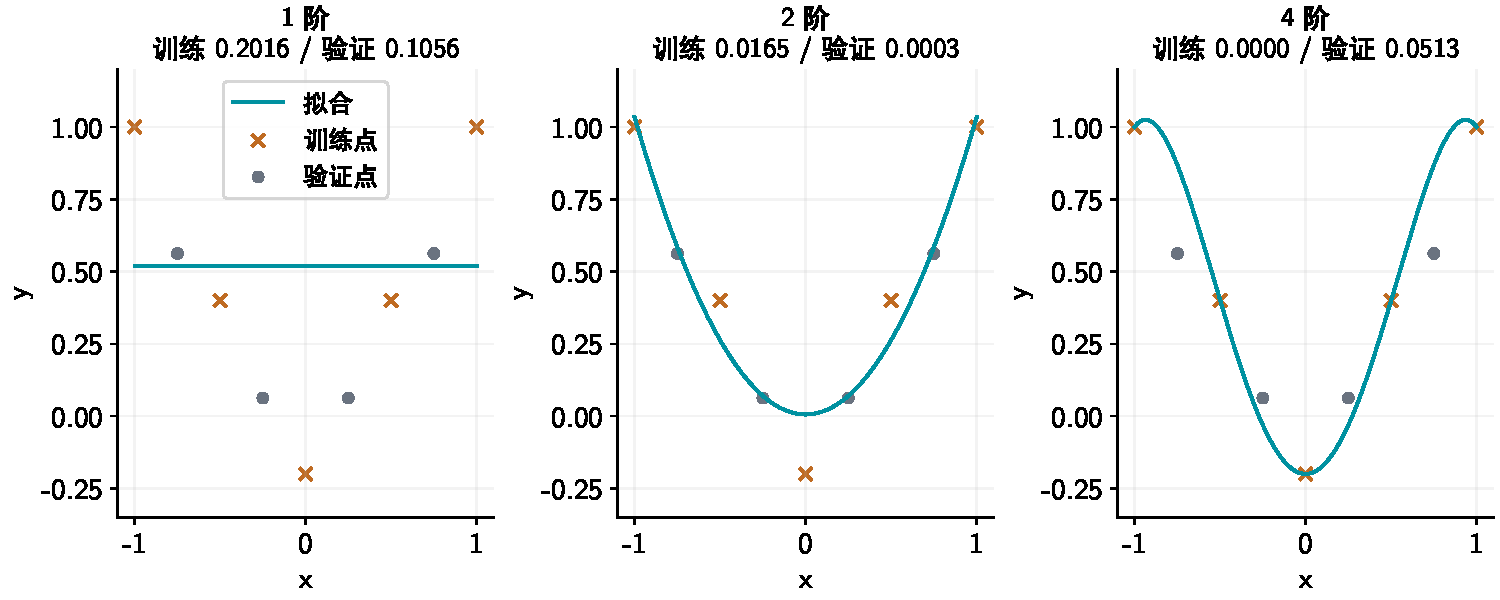
\includegraphics[width=0.98\textwidth]{images/dl_fit_revised.pdf}
\caption{同一组训练点和独立验证点的多项式实验，标出实际 MSE}
\label{fig:v2-dl-fit}
\end{figure}
欠拟合（underfitting）意味着模型连训练数据的规律都没有学好；过拟合（overfitting）则是训练表现很好，新的数据表现却差。图 \ref{fig:v2-dl-fit} 中先看训练点，再看灰色验证点。遇到后者，我们可以检查数据是否有代表性，尝试增强、正则化或早停；“把训练图片删少一些”不是通用解法。
\begin{exercise}\label{ex:v2-dl-fit}
将训练点扰动全部改成零，重新比较三个阶数的训练和验证 MSE。说明四阶模型是否一定过拟合，以及为何不能只凭模型复杂就下结论。
\end{exercise}
\begin{conclusion}
训练集用于更新参数，验证集用于选择配置与停止时机，测试集留到最后评价。训练误差小不等于泛化好，验证误差也不能证明所有赛场场景都可靠；把同一段视频的相邻帧分到训练和验证两边，很容易得到看起来漂亮的成绩。
\end{conclusion}

\subsubsection{先把 Python 环境选对}
卷一已经讲过虚拟环境。你可以继续用 Conda，也可以按下面的 venv 方法新建一个；不需要为了学习网络再配一遍整个系统。在 Distrobox 里先进入 Ubuntu，再进入工程目录。安装通用形式是 \texttt{python -m pip install [选项] 包名}；\texttt{-m pip} 使用当前解释器的包管理器，\texttt{==版本} 固定组合，\texttt{--index-url} 选择构建索引。
\begin{example}[先在 CPU 上把闭环跑通]
从项目目录执行。固定 PyTorch 2.6.0 与 torchvision 0.21.0，作为本章已验证的复现组合，不表示它们是最新版本。最后应看到解释器路径、两个版本与 \texttt{torch.Size([2,3])}。
\begin{tbash}
sudo apt install python3-venv
python3 -m venv .venv
source .venv/bin/activate
python -m pip install torch==2.6.0 torchvision==0.21.0 --index-url https://download.pytorch.org/whl/cpu
python -c "import sys,torch,torchvision; print(sys.executable,torch.__version__,torchvision.__version__,torch.ones(2,3).shape)"
\end{tbash}
\end{example}
如果终端能运行而 IDE 找不到 torch，先检查 IDE 选择的解释器是不是这个 \texttt{.venv/bin/python}。不是每个 import 错误都值得重装显卡驱动。CPU 包的 \texttt{torch.cuda.is\_available()} 为 False 很正常，需要 CUDA 时另选构建。
\begin{exercise}\label{ex:v2-dl-env}
分别在已激活与未激活虚拟环境的终端运行版本检查，记录解释器路径或实际导入错误。说明编辑器与终端版本不一致时先改哪项设置。
\end{exercise}

\subsubsection{数据：图片、标签和批量怎样配合}
MNIST 提供 60000 张训练来源图片和 10000 张测试图片，都是 $28\times28$ 手写数字灰度图，标签为 0 到 9。我们从前者固定划出 55000 张训练、5000 张验证，不拿测试集决定训练轮数。首次需要网络下载，torchvision 会校验资源；下载失败时先处理连接或缓存，不要用随机标签假装训练成功。

Dataset 保存取样规则，DataLoader 按批量（batch）交付图片与标签。ToTensor 对这里的 PIL 灰度图把 0--255 转成浮点 0--1，并增加通道维；Normalize 再按 $(x-\mathrm{mean})/\mathrm{std}$ 处理。本例沿用 MNIST 参考常数 0.1307、0.3081，没有从测试集重新估计。部署仍须使用相同处理，不是把图片 resize 成 28 就结束了。
\begin{example}[把三个集合分开]
data.py 返回三个 loader，训练打乱、评估不打乱，固定随机生成器让划分可重现。\texttt{train\_limit}=128 只缩小训练子集，验证和测试不动。后面的 train 入口直接调用它，显示首批形状。
\end{example}
\begin{dlblock}
\lstinputlisting[numbers=left,language=Python,basicstyle=\footnotesize\ttfamily,caption={data.py}]{examples/dl/lenet-training-demo/data.py}
\end{dlblock}
\begin{exercise}\label{ex:v2-dl-data}
以 \texttt{--train-limit 128 --batch-size 50 --epochs 1 --out smoke50} 运行入口。预测三个训练批量大小，核对训练样本数；解释最后一批为什么不能按 50 个样本计算平均损失。
\end{exercise}

\subsubsection{卷积、池化与激活：先算一个小窗口}
搭网络之前，我们先看看层到底做什么。卷积层（convolution layer）用可训练的核提取局部特征。同一个核在不同位置复用参数，各输出通道使用自己的核；多输入通道还要把各通道结果求和并加偏置。Conv2d 实际使用不翻转核的互相关（cross-correlation）约定，工程里仍习惯叫卷积。图 \ref{fig:v2-dl-conv} 的左上输出为 19，你可以拿四个乘法核对，不必先背一页公式。
\begin{equation}
Y_{o,i,j}=b_o+\sum_c\sum_{a=0}^{k_h-1}\sum_{b=0}^{k_w-1}
 W_{o,c,a,b}X_{c,is_h+a-p_h,js_w+b-p_w}.
\end{equation}
越界位置按零填充处理。膨胀率为 1 时，高度输出为
$\left\lfloor(n_h+2p_h-k_h)/s_h\right\rfloor+1$，宽度同理；$p_h$ 是每侧填充量，$s_h$ 是步幅（stride）。核不必是奇数，图中 $2\times2$ 就能算，只是 $3\times3$、$5\times5$ 很常见。
\begin{figure}[H]
\centering
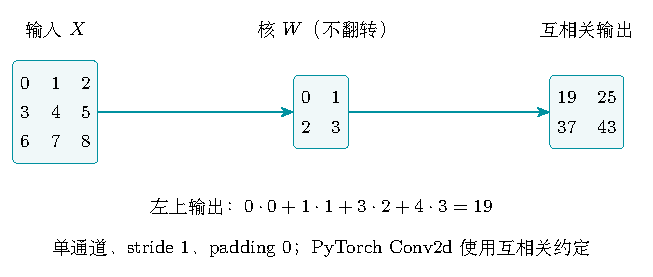
\includegraphics[width=0.9\textwidth]{images/dl_conv_revised.pdf}
\caption{不翻转核的互相关，保留原图的输入、核与输出数值}
\label{fig:v2-dl-conv}
\end{figure}
池化层（pooling layer）也滑动窗口，不过没有这里的可训练核权重：最大池化取最大值，平均池化取平均值。它常用于减少空间尺寸，对局部位置变化有一定容忍，但不保证任意平移后结果都相同。图 \ref{fig:v2-dl-pool} 两个结果分别来自原输入，窗口是 $2\times2$、步幅是 1；本章网络中步幅为 2，别照抄图的尺寸。
\begin{figure}[H]
\centering
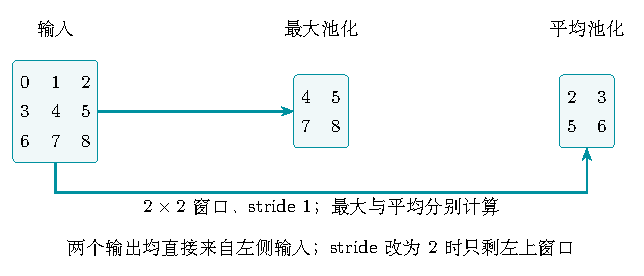
\includegraphics[width=0.9\textwidth]{images/dl_pool_revised.pdf}
\caption{同一输入的最大和平均池化，右侧不是再处理中间结果}
\label{fig:v2-dl-pool}
\end{figure}
激活函数（activation function）引入非线性。只叠多个线性层而不加非线性，最终仍能合并为一个仿射变换。我们用 ReLU（rectified linear unit，修正线性单元）：$\mathrm{ReLU}(x)=\max(0,x)$，负输入输出零，不是删除参数。另一个常见函数 $\mathrm{sigmoid}(x)=1/(1+e^{-x})$ 把有限实数压到 0--1 之间；本章多类别输出没有使用它。
\begin{example}[公式算完，让程序再算一次]
运行 \texttt{python ops\_demo.py}，互相关为 19/25/37/43，最大池化为 4/5/7/8，平均为 2/3/5/6；随后比较两种激活对负数、零、正数的结果。
\end{example}
\begin{dlblock}
\lstinputlisting[numbers=left,language=Python,caption={ops\_demo.py}]{examples/dl/lenet-training-demo/ops_demo.py}
\end{dlblock}
\begin{exercise}\label{ex:v2-dl-ops}
把两个池化调用的步幅改为 2，预测尺寸和数值后运行；再将核改为全 1，核对互相关。两次修改分别保存，不要把窗口、步幅和核一起改得认不出来。
\end{exercise}

\subsubsection{搭建 LeNet：每一层都能对上形状}
现在我们把这些层串起来。nn.Module 管理参数与子模块，\texttt{\_\_init\_\_} 创建层，forward 定义数据经过它们的顺序。本例是 LeNet 风格的教学网络，两组卷积/ReLU/最大池化后接三个全连接层（fully connected layer）；没有照搬原始 LeNet-5 的激活、汇聚和输出形式。旧图常见的是 32 输入，本章 MNIST 为 28 输入，图 \ref{fig:v2-dl-lenet} 将两条尺寸链分开了。

Conv2d(1,6,5) 的位置参数是输入通道、输出通道和核大小；MaxPool2d(2) 默认步幅等于核大小。尺寸为 $28\to24\to12\to8\to4$，一个样本最终有 $16\times4\times4=256$ 个特征。flatten(1) 保留第零维批量，展平其余维；Linear(84,10) 给十类输出未归一化分数（logits），暂时没有概率。
\begin{figure}[H]
\centering
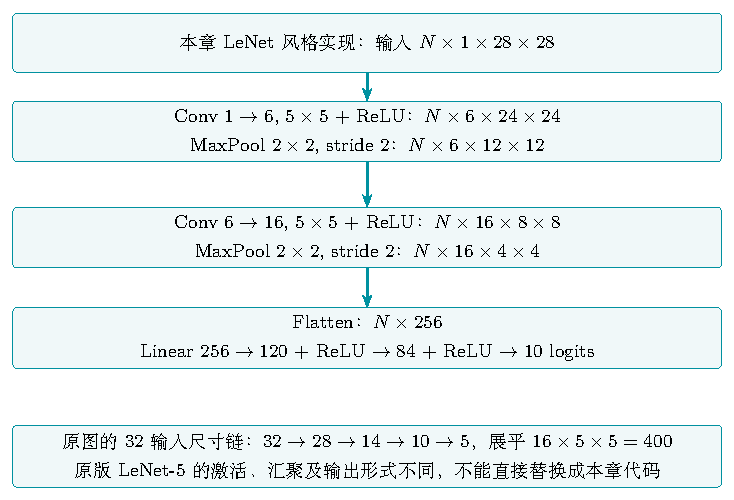
\includegraphics[width=0.92\textwidth]{images/dl_lenet_revised.pdf}
\caption{本章形状与原图 32 输入的区别，$N$ 为批量大小}
\label{fig:v2-dl-lenet}
\end{figure}
\begin{example}[先前向，再训练]
运行 \texttt{python model.py}，看到特征 \texttt{(2,16,4,4)}、展平 \texttt{(2,256)}、分数 \texttt{(2,10)}。Sequential 将连续层组合为容器，作用与同序逐个调用一致；特征与分类器分开，方便你检查中间形状。
\end{example}
\begin{dlblock}
\lstinputlisting[numbers=left,language=Python,basicstyle=\footnotesize\ttfamily,caption={model.py}]{examples/dl/lenet-training-demo/model.py}
\end{dlblock}
\begin{exercise}\label{ex:v2-dl-shape}
将入口输入改为 $32\times32$，记录特征与展平形状，再看分类器报错。手算并修改第一层 Linear 输入数，使它输出 \texttt{(2,10)}；此变体不要覆盖后面的 28 输入模型。
\end{exercise}

\subsubsection{损失、反向传播和优化器各做什么}
前向能输出分数，不过随机参数还不会认数字。损失函数（loss function）衡量预测与标签的差距，反向传播（backpropagation）按链式法则计算参数梯度，优化器（optimizer）才用梯度更新参数。这三步不要混成“调用 backward 就学会了”。

本章交叉熵（cross entropy）针对单个正确类别 $y$：
$L=-\log\bigl(e^{z_y}/\sum_j e^{z_j}\bigr)$，$z$ 是 logits。CrossEntropyLoss 内部完成稳定的 log-softmax，给它整数标签与原分数；你若先 softmax，就让它把概率又当分数处理，损失含义变了。
\begin{example}[分数、概率和损失别重复加工]
运行 \texttt{python loss\_demo.py}，交叉熵与负对数正确类概率一致，约 0.16985；提前 softmax 后约 0.65785。随后打印的是分数梯度，不是更新后的分数。
\end{example}
\begin{dlblock}
\lstinputlisting[numbers=left,language=Python,caption={loss\_demo.py}]{examples/dl/lenet-training-demo/loss_demo.py}
\end{dlblock}
简单梯度下降为 $\theta\leftarrow\theta-\eta\nabla_\theta L$，学习率（learning rate）$\eta$ 控制步长。我们先用一个参数算清楚，再在网络中使用 Adam。Adam 用梯度的一、二阶矩估计调整更新量，不保证必然稳定或达到全局最优；学习率、批量与轮数仍按验证结果选择。
\begin{example}[梯度算出来了，参数还没动]
\texttt{grad\_demo} 的 $w=0$、$L=(2w-4)^2$，第一次梯度 -16；重新建图反传但不清梯度，变为 -32。清零后以学习率 0.1 更新一步，$w=1.6$、损失约 0.64。运行 \texttt{python grad\_demo.py} 核对三次状态。
\end{example}
\begin{dlblock}
\lstinputlisting[numbers=left,language=Python,caption={grad\_demo.py}]{examples/dl/lenet-training-demo/grad_demo.py}
\end{dlblock}
\begin{exercise}\label{ex:v2-dl-grad}
把 SGD 学习率改为 0.05，手算清零后一步的参数和损失，再运行。说明保留 -32 梯度会有什么不同，以及 backward 与 step 的分工。
\end{exercise}

\subsubsection{训练与评估：不用训练时的状态考自己}
每批先清梯度，前向求分数和损失，再反传、更新；评估只前向统计。engine 将两者放在同一函数，是否传入 optimizer 决定行为。损失按样本数累加，因为最后一批可能较小，直接平均每批均值会给小批量同样的权重。

train/eval 改变 Dropout、BatchNorm 等层行为，\texttt{no\_grad} 关闭梯度记录，两者不是同一开关。本例 LeNet 没有这两类层，数值可能看不出区别，但仍保留正确评估路径，否则以后换网络就容易踩坑。
\begin{example}[两个开关分开看]
运行 \texttt{python mode\_demo.py}。训练状态即使在 \texttt{no\_grad} 中，Dropout 仍将部分输入置零并缩放；eval 输出全 1，但输入需要梯度时仍保留梯度关系。代码在 Dropout 后 clone 一次，避免 p=0 直接返回原输入时把原输入的 \texttt{requires\_grad} 误当作新计算图。eval 与 \texttt{no\_grad} 一起使用才是此处推理状态。
\end{example}
\begin{dlblock}
\lstinputlisting[numbers=left,language=Python,caption={mode\_demo.py}]{examples/dl/lenet-training-demo/mode_demo.py}
\end{dlblock}
\begin{example}[一套循环负责训练和验证]
下面的 engine 被 train 实际调用。评估不会清梯度、反传或更新，也不记录计算图；统计返回样本数，能与集合大小对照。完整运行紧接在入口后。
\end{example}
\begin{dlblock}
\lstinputlisting[numbers=left,language=Python,basicstyle=\footnotesize\ttfamily,caption={engine.py}]{examples/dl/lenet-training-demo/engine.py}
\end{dlblock}
\begin{exercise}\label{ex:v2-dl-mode}
将 Dropout 概率改为 0，重复三种状态。输出相同是否说明两个开关可以互相代替？指出 engine 控制层状态和梯度记录的两条语句。
\end{exercise}
\begin{conclusion}
forward 给预测，loss 衡量差距，backward 算梯度，step 更新参数，\texttt{zero\_grad} 防止意外累加。train/eval 控制层行为，梯度记录另有开关。训练保留反向所需中间值，较大批量或网络可能占用更多内存/显存；显存不足时先缩小批量并检查是否留住了旧计算图，不能只看参数文件大小。
\end{conclusion}

\subsubsection{完整入口：小批量检查，再恢复训练}
文件职责已经清楚了：data 给集合，model 给结构，engine 执行一轮，train 配置、选模型与保存，infer 在另一进程使用结果。其他 demo 只为了缩小观察难点，不参与主线训练。项目目录如下：
\begin{tbash}
lenet-training-demo/
  model.py  data.py  engine.py  train.py  infer.py
  fit_demo.py  ops_demo.py  loss_demo.py  grad_demo.py  mode_demo.py
  device_demo.py  nms_demo.py  export_compare.py  benchmark.py
  requirements-export.txt  README.md
\end{tbash}
入口前半段的 --data 是缓存目录，--out 是结果目录，默认 CPU、一个线程、批量 64、三轮；train-limit 0 是完整训练子集。先移动模型，再创建优化器，每批输入与标签也移到同一设备。固定种子便于本机对照，不保证跨设备和版本逐位相同。
\begin{dlblock}
\lstinputlisting[numbers=left,language=Python,firstline=1,lastline=40,basicstyle=\footnotesize\ttfamily,caption={train.py：参数与准备}]{examples/dl/lenet-training-demo/train.py}
\end{dlblock}
后半段逐轮记录训练与验证，只在验证损失改善时保存。结束后载入选中的参数，最后评价一次测试集；测试没有回头影响选择。除了权重，还保存结构名称、归一化与类别表，避免留下不知道怎样使用的“存档”。metrics.json 记录版本、配置与曲线。
\begin{dlblock}
\lstinputlisting[numbers=left,language=Python,firstline=41,firstnumber=41,basicstyle=\footnotesize\ttfamily,caption={train.py：选模型、保存与最终评价}]{examples/dl/lenet-training-demo/train.py}
\end{dlblock}
\begin{example}[先确认代码能绕回来]
从工程目录执行。128 张一轮的首批为 \texttt{(64,1,28,28)}、标签 \texttt{(64,)}、输出 \texttt{(64,10)}；随后恢复完整训练。每轮 train 记录为 55000 样本，valid 为 5000，最终 test 为 10000。
\begin{tbash}
python train.py --epochs 1 --train-limit 128 --out smoke
python train.py --epochs 3 --out runs
python infer.py --index 0 1 2
\end{tbash}
\end{example}
\begin{note}
再次用同一输出目录会覆盖 best.pth 与 metrics.json，比较实验请换 --out。128 张只检查流程，准确率低不说明环境坏了，也别凭这点样本给模型下结论。训练启动后无需一直按运行按钮，等一轮统计出来再判断。
\end{note}
\begin{figure}[H]
\centering
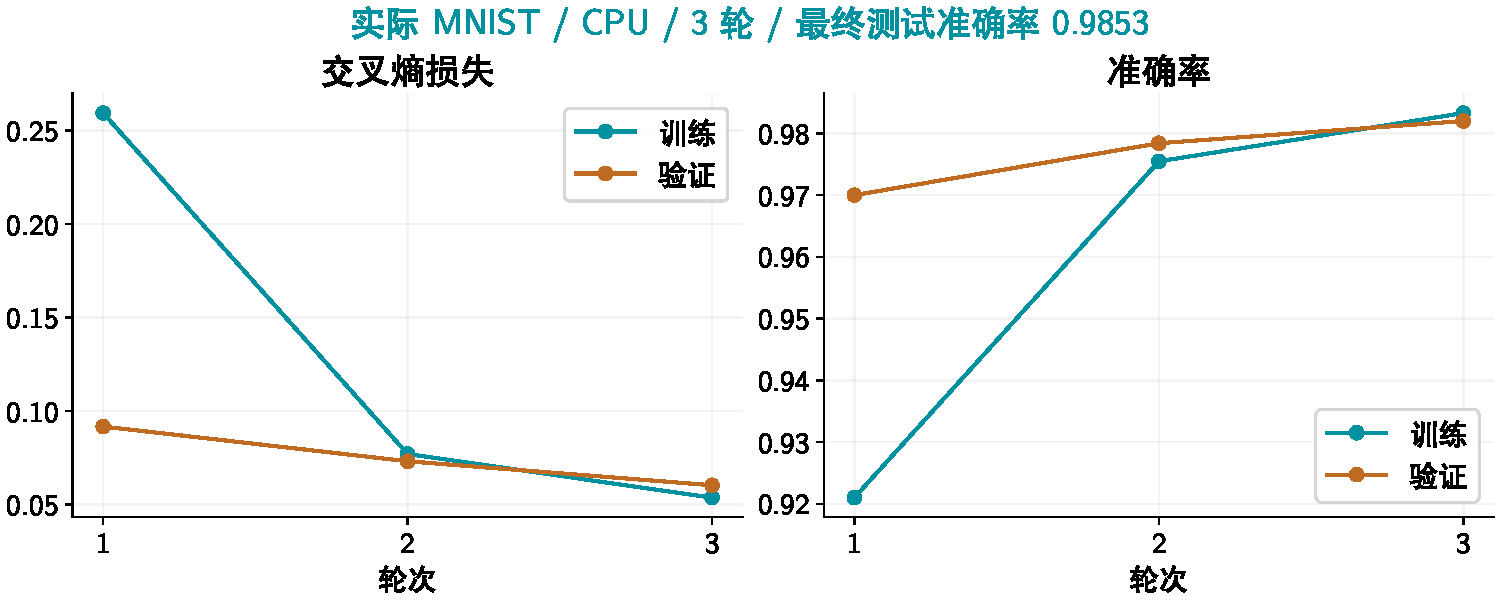
\includegraphics[width=0.96\textwidth]{images/dl_curve_revised.pdf}
\caption{本次 CPU 三轮完整训练的真实记录，成绩随版本与配置变化}
\label{fig:v2-dl-curve}
\end{figure}
图 \ref{fig:v2-dl-curve} 来自 Ubuntu 24.04/PyTorch 2.6.0 CPU 实际运行，最终测试准确率 0.9853。它说明此教学任务的结果，不证明装甲板数字也能直接识别；真实数据的裁剪、类别、模糊和光照不同，赛场训练见卷三。
\begin{exercise}\label{ex:v2-dl-train}
完成小规模与完整训练，记录版本、集合样本数及每轮验证损失。根据 metrics 判断保存哪一轮，解释只看最后一轮训练损失为什么不能替代这个选择。
\end{exercise}

\subsubsection{保存与加载：参数还需要使用说明}
参数文件有了，不过 \texttt{state\_dict} 主要是参数与持久缓冲，不替你保存完整网络定义、预处理和类别含义。加载时先创建相同结构，再填参数；仅把后缀从 .pth 改成 .onnx 可不会施展格式转换魔法。

infer 使用保存的结构标记与归一化，对指定测试样本输出十个分数和预测类别，取最大分数索引。想显示概率时再 softmax，概率大小也不自动等于校准后的可靠程度。\texttt{map\_location}='cpu' 让 CUDA 权重能在 CPU 读取，\texttt{weights\_only}=True 限制加载形式；仍应使用自己训练或可信来源的文件。
\begin{example}[换一个进程读存档]
运行 \texttt{python infer.py --index 0 1 2}，三行给索引、真标签、预测与分数。检查者可指定 0--9999 索引。--checkpoint 换权重路径，--data 与训练缓存一致，不需要再训练。
\end{example}
\begin{dlblock}
\lstinputlisting[numbers=left,language=Python,firstline=1,lastline=16,basicstyle=\footnotesize\ttfamily,caption={infer.py：结构与参数}]{examples/dl/lenet-training-demo/infer.py}
\end{dlblock}
\begin{dlblock}
\lstinputlisting[numbers=left,language=Python,firstline=17,firstnumber=17,basicstyle=\footnotesize\ttfamily,caption={infer.py：指定样本与分数}]{examples/dl/lenet-training-demo/infer.py}
\end{dlblock}
\begin{exercise}\label{ex:v2-dl-load}
复制 model，将第一层 Linear 输入改为 400，再在变体工程用原权重运行 infer，记录报错。恢复结构后核对同一图片输出，说明改变归一化为什么可能不报错却改变预测。
\end{exercise}

\subsubsection{选用 CUDA：先确认构建和设备，再谈速度}
如果有可用 NVIDIA 显卡，可选 PyTorch CUDA 构建，让相同循环使用 GPU。CPU 包不会因装了驱动就变成 CUDA 包；PyTorch 附带的运行库也不是下一章的完整 nvcc 工具链。先查驱动，再从 \href{https://docs.pytorch.org/get-started/previous-versions/}{官方固定版本组合}选匹配构建，建议保留能用的 CPU 环境。
\begin{example}[本机可用时走相同训练路径]
在新环境安装下面已验证的组合，再进入相同工程。前提是驱动与容器能使用此 CUDA 构建。不能使用的机器继续 CPU 主线。
\begin{tbash}
python3 -m venv .venv-cuda
source .venv-cuda/bin/activate
python -m pip install torch==2.6.0 torchvision==0.21.0 --index-url https://download.pytorch.org/whl/cu126
python -c "import torch; print(torch.__version__,torch.version.cuda,torch.cuda.is_available())"
python train.py --epochs 1 --train-limit 128 --device cuda --out gpu-smoke
python device_demo.py
\end{tbash}
\end{example}
\texttt{device\_demo} 用主线 runs/best.pth 的相同参数与输入比较 CPU/CUDA，不拿两个随机网络硬比。本次 Distrobox 的 RTX 3070 Ti Laptop GPU 实际跑通 CUDA 12.6 构建；其他设备仍按实际检查。没有传输、预热与同步的计时，不能证明 GPU 更快。
\begin{dlblock}
\lstinputlisting[numbers=left,language=Python,caption={device\_demo.py}]{examples/dl/lenet-training-demo/device_demo.py}
\end{dlblock}
\begin{exercise}\label{ex:v2-dl-device}
记录两个环境的版本与可用性；有设备时跑 gpu-smoke 和同参数比较，提交设备名与误差。无设备时指出 train 移动模型、输入、标签的位置，如实写未完成 GPU 实测。
\end{exercise}

\subsubsection{从分类到检测：框还要解码和去重}
数字分类只输出类别分数，机器人检测还要告诉我们物体在哪。YOLO（You Only Look Once）是一类检测方法和多个实现的名字，不是永远相同的架构。图 \ref{fig:v2-dl-yolo} 保留原图历史 YOLOv5s 的 Focus/CSP/SPP、多尺度融合与三个预测尺度，用 \href{https://github.com/ultralytics/yolov5/blob/v1.0/models/yolov5s.yaml}{v1.0 配置}定位；608 输入对应 76、38、19 网格，255 来自三组 anchor 和 80 类，不能直接套任意新版。
\begin{figure}[H]
\centering
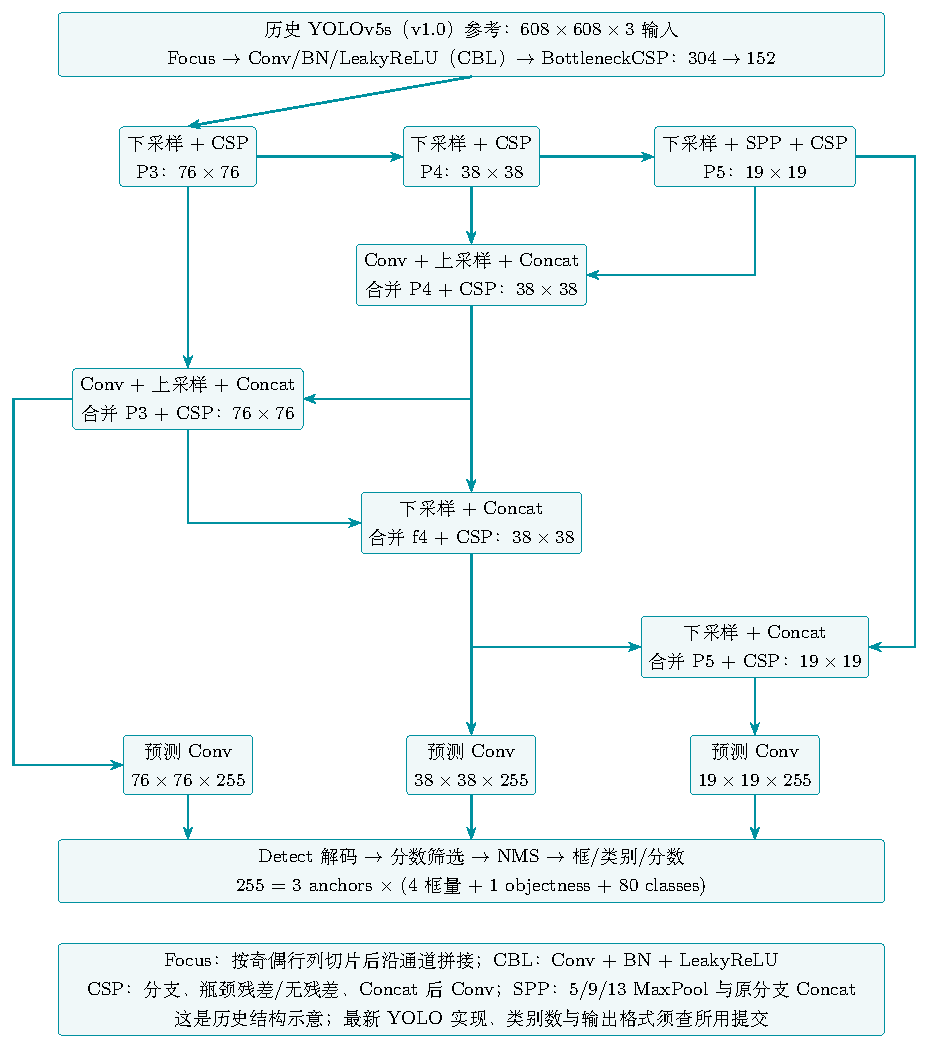
\includegraphics[width=0.88\textwidth]{images/dl_yolo_revised.pdf}
\caption{历史 YOLOv5s 的多尺度路径和模块含义，不是本章训练网络}
\label{fig:v2-dl-yolo}
\end{figure}
用现成框架仍须核对提交、许可、类别表、颜色与归一化、缩放/补边、输出解码。网络给候选框后，常用非极大值抑制（non-maximum suppression，NMS）去掉同类高重叠框；交并比（intersection over union，IoU）是交集面积除以并集面积。分数高不等于框正确，NMS 也不负责修错分类。
\begin{example}[三个同类框的去重]
运行 \texttt{python nms\_demo.py}，保留索引 0、2。前两个框 IoU 为 $81/119\approx0.681$，低分框被抑制；第三个在另一处。这是人工候选框后处理，没有训练好的 YOLO 权重，不要当检测成绩。
\end{example}
\begin{dlblock}
\lstinputlisting[numbers=left,language=Python,caption={nms\_demo.py}]{examples/dl/lenet-training-demo/nms_demo.py}
\end{dlblock}
\begin{exercise}\label{ex:v2-dl-nms}
将 IoU 阈值改为 0.8，预测保留索引后运行。说明改变的是去重条件还是网络预测；不同类别的重叠框能否直接沿用这个同类示例。
\end{exercise}

\subsubsection{部署入口：先核对数值，再测用时}
机器人程序可能使用不同语言、运行时和硬件。ONNX（Open Neural Network Exchange）用于交换计算图，OpenVINO、TensorRT 等可为目标设备转换或优化；算子支持、尺寸、精度与速度仍由实际模型和设备决定。.pth/.pt 常见于 PyTorch 保存，OpenVINO IR 常见 .xml/.bin，TensorRT 引擎常见 .engine，这些不能靠改名互换。

先做能核验的导出。依赖集中在 \path{requirements-export.txt}，固定 onnx 1.17.0 与 onnxruntime 1.20.1。随后 \texttt{export\_compare} 从主线权重读结构、预处理，用同一真实测试图分别在 PyTorch 与 CPU ONNX Runtime 前向，比较完整分数。输入固定 $1\times1\times28\times28$、opset 17；dynamo=False 明确此次实测路径，不靠新版默认值猜行为。
\begin{dlblock}
\lstinputlisting[numbers=left,caption={requirements-export.txt}]{examples/dl/lenet-training-demo/requirements-export.txt}
\end{dlblock}
\begin{example}[导出成功还要比较]
在 CPU 环境、项目目录执行。结果显示 \texttt{[1,10]}、最大绝对误差与类别，满足代码容差。默认写到已有 runs，换 --output 时确保父目录存在。
\begin{tbash}
python -m pip install -r requirements-export.txt
python export_compare.py
\end{tbash}
\end{example}
\begin{dlblock}
\lstinputlisting[numbers=left,language=Python,firstline=1,lastline=24,basicstyle=\footnotesize\ttfamily,caption={export\_compare.py：同一预处理输入}]{examples/dl/lenet-training-demo/export_compare.py}
\end{dlblock}
\begin{dlblock}
\lstinputlisting[numbers=left,language=Python,firstline=25,firstnumber=25,basicstyle=\footnotesize\ttfamily,caption={export\_compare.py：图与完整输出误差}]{examples/dl/lenet-training-demo/export_compare.py}
\end{dlblock}
onnx.checker 检查图，数值比较检查这些输入的实际输出，不能证明所有输入正确。当前图未包含外部预处理，部署须保存 mean/std、颜色、尺寸与类别表。查看结构可用 \href{https://netron.app/}{Netron}，导出限制查 \href{https://docs.pytorch.org/docs/2.6/onnx.html}{本章版本的导出文档}；结构能打开不是部署完成。

然后测 CPU 前向。计时器（benchmark）预热并多次测量，以中位数减少偶然波动；固定一个线程，比较批量 1 与 32。每样本成本与吞吐率说明批处理效率，单帧响应还包含预处理、排队、传输和后处理。CUDA 异步提交也不能直接用普通时钟相减测完整 GPU 用时，需要同步或事件计时。
\begin{example}[同一模型比较两个批量]
在有主线权重的 CPU 工程运行 \texttt{python benchmark.py}，报告每批毫秒、每样本毫秒、每秒样本数与线程数，不预先承诺快多少。
\end{example}
\begin{dlblock}
\lstinputlisting[numbers=left,language=Python,caption={benchmark.py}]{examples/dl/lenet-training-demo/benchmark.py}
\end{dlblock}
\begin{exercise}\label{ex:v2-dl-deploy}
换测试索引 1、2 分别导出比较，记录误差与类别。再把 benchmark 批量 32 改为 8，报告三个时间/吞吐指标，说明此计时没覆盖哪些单帧工作。
\end{exercise}
\begin{conclusion}
参数需要结构与预处理，交换图需要算子、尺寸与数值检查，部署还需要目标运行时、后处理与端到端计时。本章跑通 CPU ONNX Runtime 固定输入对照，OpenVINO/TensorRT 是后续目标，未实测就不写加速完成。
\end{conclusion}
到这里，我们能训练小网络、存下参数、在新进程识别指定样本，并跨运行时核对输出。神经网络在自瞄数字、装甲板与雷达感知中都有用，不过下一步应换成代表性真实数据与明确任务。想继续看自动求导与数据加载，可以顺着 \href{https://docs.pytorch.org/tutorials/beginner/basics/}{PyTorch 官方基础教程}查，先把当前闭环解释清楚再加新框架。


\section{本章小结}
我们从手写规则走到数据学习，先用独立验证点区分拟合与泛化，再把图片与标签分成训练、验证和测试。卷积、池化与激活组成特征，展平后用全连接输出 logits；损失给出差距，反向传播求梯度，优化器才更新参数。训练先用少量数据检查闭环，再恢复完整集合，按验证损失保存模型，最后才评价测试集。

你应能熟练核对输入、每层形状、设备与训练状态，保存结构、预处理和类别说明，重新载入指定样本并解释分数。检测还需要框解码与后处理，换运行时要核对完整数值，再测用时；现成检测框架、OpenVINO/TensorRT 的具体支持和赛场数据继续查对应版本与卷三，不能凭文件后缀或算力推断效果。

\begin{problemset}
\item\label{prob:v2-dl-1} 基础：训练误差下降而验证误差上升，优先检查什么？同一段视频的相邻帧被随机分到训练与验证，会怎样影响评价？
\item\label{prob:v2-dl-2} 基础：输入 $3\times10\times10$、输出 8 通道、$3\times3$ 核、每侧填充 1、步幅 2 的卷积，输出形状与参数数目（含偏置）是多少？
\item\label{prob:v2-dl-3} 基础：28 输入的本章网络为什么有 256 个展平特征？把 batch 从 1 改成 8，需要将 Linear 输入数乘以 8 吗？
\item\label{prob:v2-dl-4} 基础：logits、softmax 概率与交叉熵是什么关系？backward 后参数是否已更新，第二次 backward 是否自动清梯度？
\item\label{prob:v2-dl-5} 基础：eval 与 \texttt{no\_grad} 分别控制什么？本章 LeNet 没有 Dropout/BatchNorm，是否就可以永远不写 eval？
\item\label{prob:v2-dl-6} 基础：交付 best.pth 还需要哪些说明？输入形状一致是否足以证明两个预处理流程等效？
\item\label{prob:v2-dl-7} 提高：驱动可用但 \texttt{torch.cuda.is\_available} 为 False，应先检查什么？GPU 前向只测普通时钟间隔为什么可能低估时间？
\item\label{prob:v2-dl-8} 提高：历史 YOLOv5 的 255 个预测通道代表什么？改成 3 类时该通道数是多少？同类 NMS 能否不加区分地用于不同类？
\item\label{prob:v2-dl-9} 提高：本章 ONNX 文件能直接输入批量 8 吗？导出检查通过、某张图类别相同，是否足以宣布部署一致？
\item\label{prob:v2-dl-10} 实践：独立加载训练选中的参数，对检查者指定的三个测试索引输出分数；其中一个再跨运行时比较。提交结构、预处理、类别、误差与 CPU 前向计时，并说明实机单帧响应还缺什么。
\end{problemset}

\section{本章验收}
\begin{enumerate}
  \item 从独立环境运行小规模与完整 MNIST 训练，展示版本、首批形状、三个集合大小、逐轮曲线及最终测试；说明参数选择没有使用测试集。
  \item 现场改变卷积/池化步幅或输入尺寸，手算并验证输出，解释维度错误；展示梯度计算、累加、清零与更新的区别。
  \item 在另一进程加载最佳参数，对指定索引推理，解释预处理与类别表；有 CUDA 时展示同参数输出比较，无设备如实记录缺口。
  \item 对同一真实输入比较 PyTorch 与 ONNX Runtime 完整分数，检查输入限制并展示 CPU 批量计时，区分推理成本、吞吐与相机端到端响应。
\end{enumerate}


% ============================================================
\chapter{CUDA 与 GPU 加速}

\begin{introduction}
  \item 学习目标：核对驱动、编译器与运行库；构建 CUDA 工程；验证索引、共享归约和错误；比较含传输的流水线计时。
  \item 建议学时：约 3--5 天。
  \item 本卷边界：先修卷一 C++ 与 CMake；本章训练 GPU 基础编程，项目级推理部署与赛场性能指标见卷三。
\end{introduction}

\section{环境与并行编程}

\section{CUDA 简介}

2006 年，NVIDIA 发布 \textbf{CUDA}（Compute Unified Device Architecture）：
一套在 NVIDIA GPU 上做通用并行计算的平台与编程模型。
与必须把计算映射到图形 API 不同，CUDA 把 GPU 当作数据并行计算设备，
用接近 C/C++ 的语法编写在设备端执行的函数（\textbf{kernel}）。

视觉组相关用途主要包括：
\begin{itemize}
    \item 图像预处理、滤波、几何变换等可高度并行的算子；
    \item 深度学习训练与推理的底层加速（PyTorch、TensorRT 等均依赖 CUDA）；
    \item 自定义高性能算子（当库函数无法满足延迟要求时）。
\end{itemize}

配套库常见有：运行时 API、\textbf{cuBLAS}（线性代数）、\textbf{cuFFT}（FFT）、
\textbf{cuDNN}（深度网络原语）等。官方文档见
\url{https://docs.nvidia.com/cuda/cuda-programming-guide/}。

\section{配置 CUDA 环境}

版本需与显卡驱动、Ubuntu 发行版匹配。安装前先确认驱动：
\begin{tbash}
nvidia-smi
\end{tbash}
能显示 GPU 型号与 Driver Version 再继续；无输出则先装专有驱动。

\subsection{安装 CUDA Toolkit}

下面以 Ubuntu 22.04 + CUDA 11.8 的 \texttt{.run} 安装为例（版本号请按官网当前推荐调整）。

\begin{tbash}
wget https://developer.download.nvidia.com/compute/cuda/11.8.0/local_installers/cuda_11.8.0_520.61.05_linux.run
sudo sh cuda_11.8.0_520.61.05_linux.run
\end{tbash}

\begin{figure}[H]
    \centering
    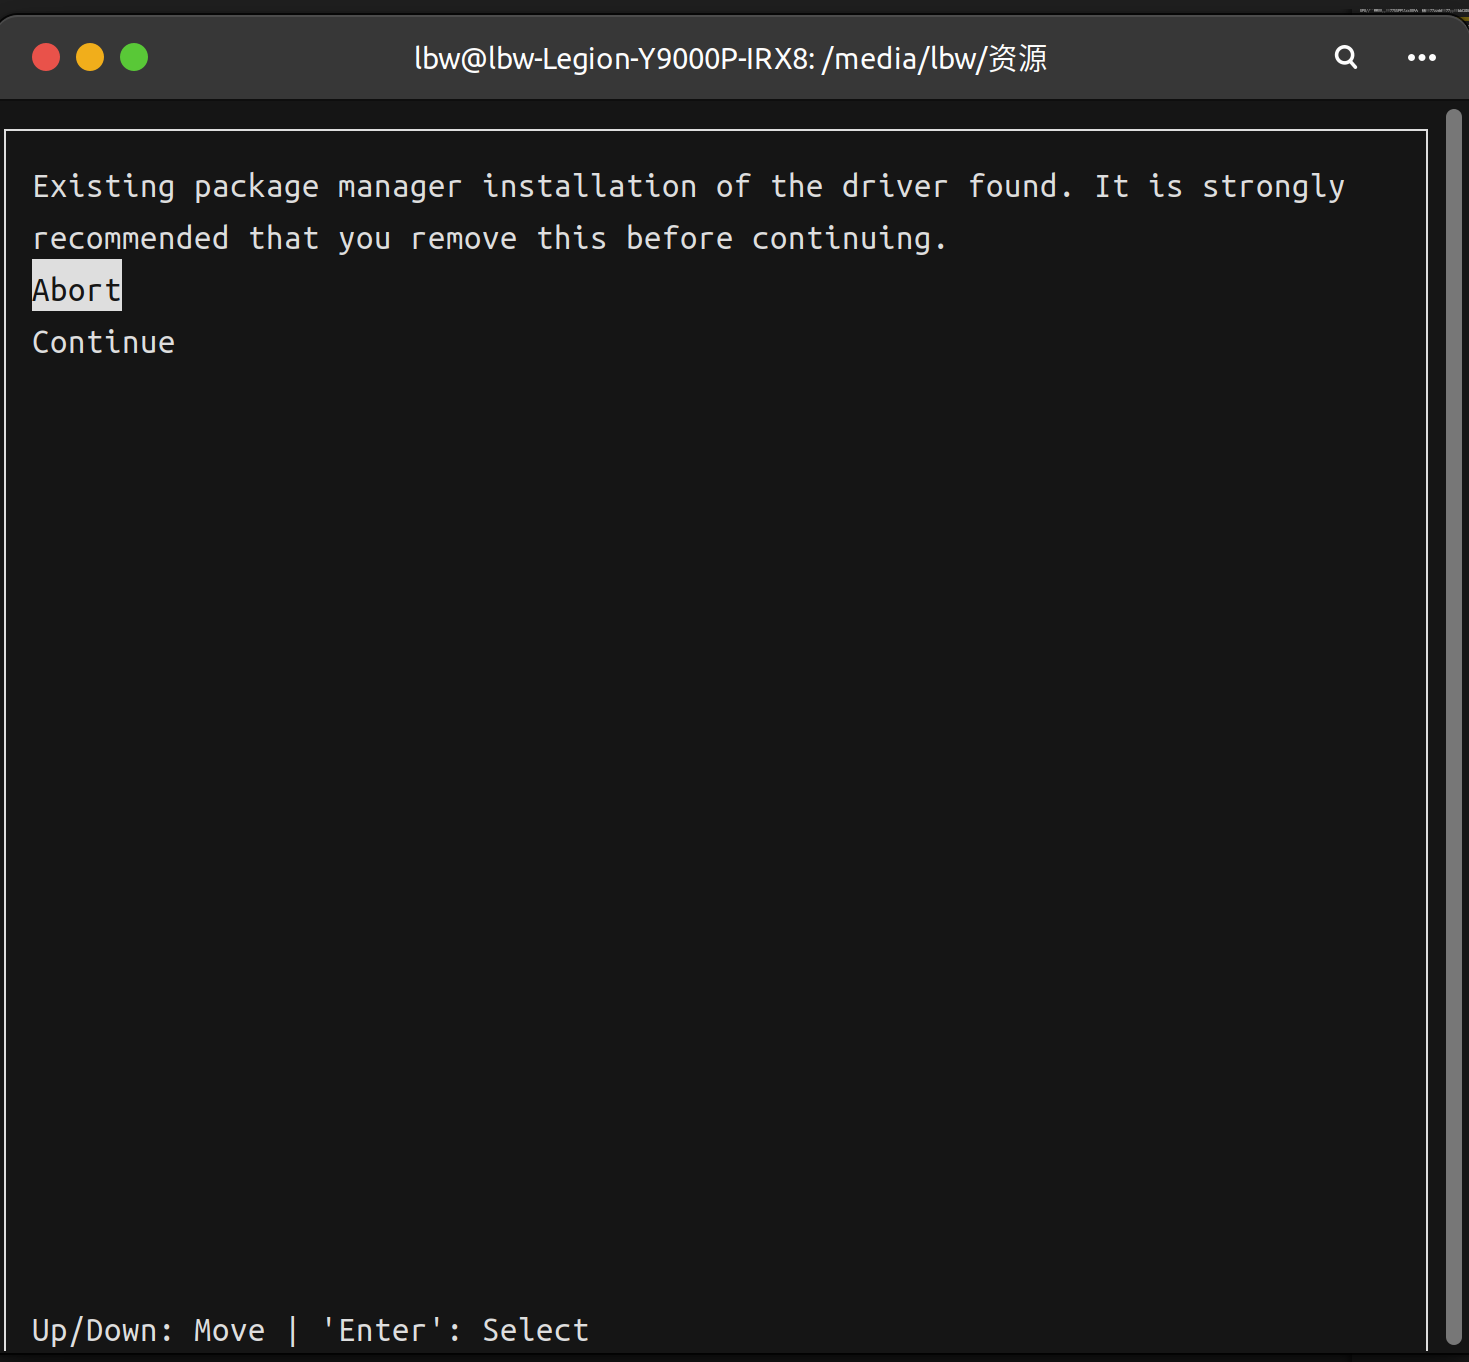
\includegraphics[width=0.7\textwidth]{CUDA_install.png}
    \caption{CUDA 安装向导}
    \label{fig:cuda_install1}
\end{figure}

选择 Continue，接受许可后进入组件选择：

\begin{figure}[H]
    \centering
    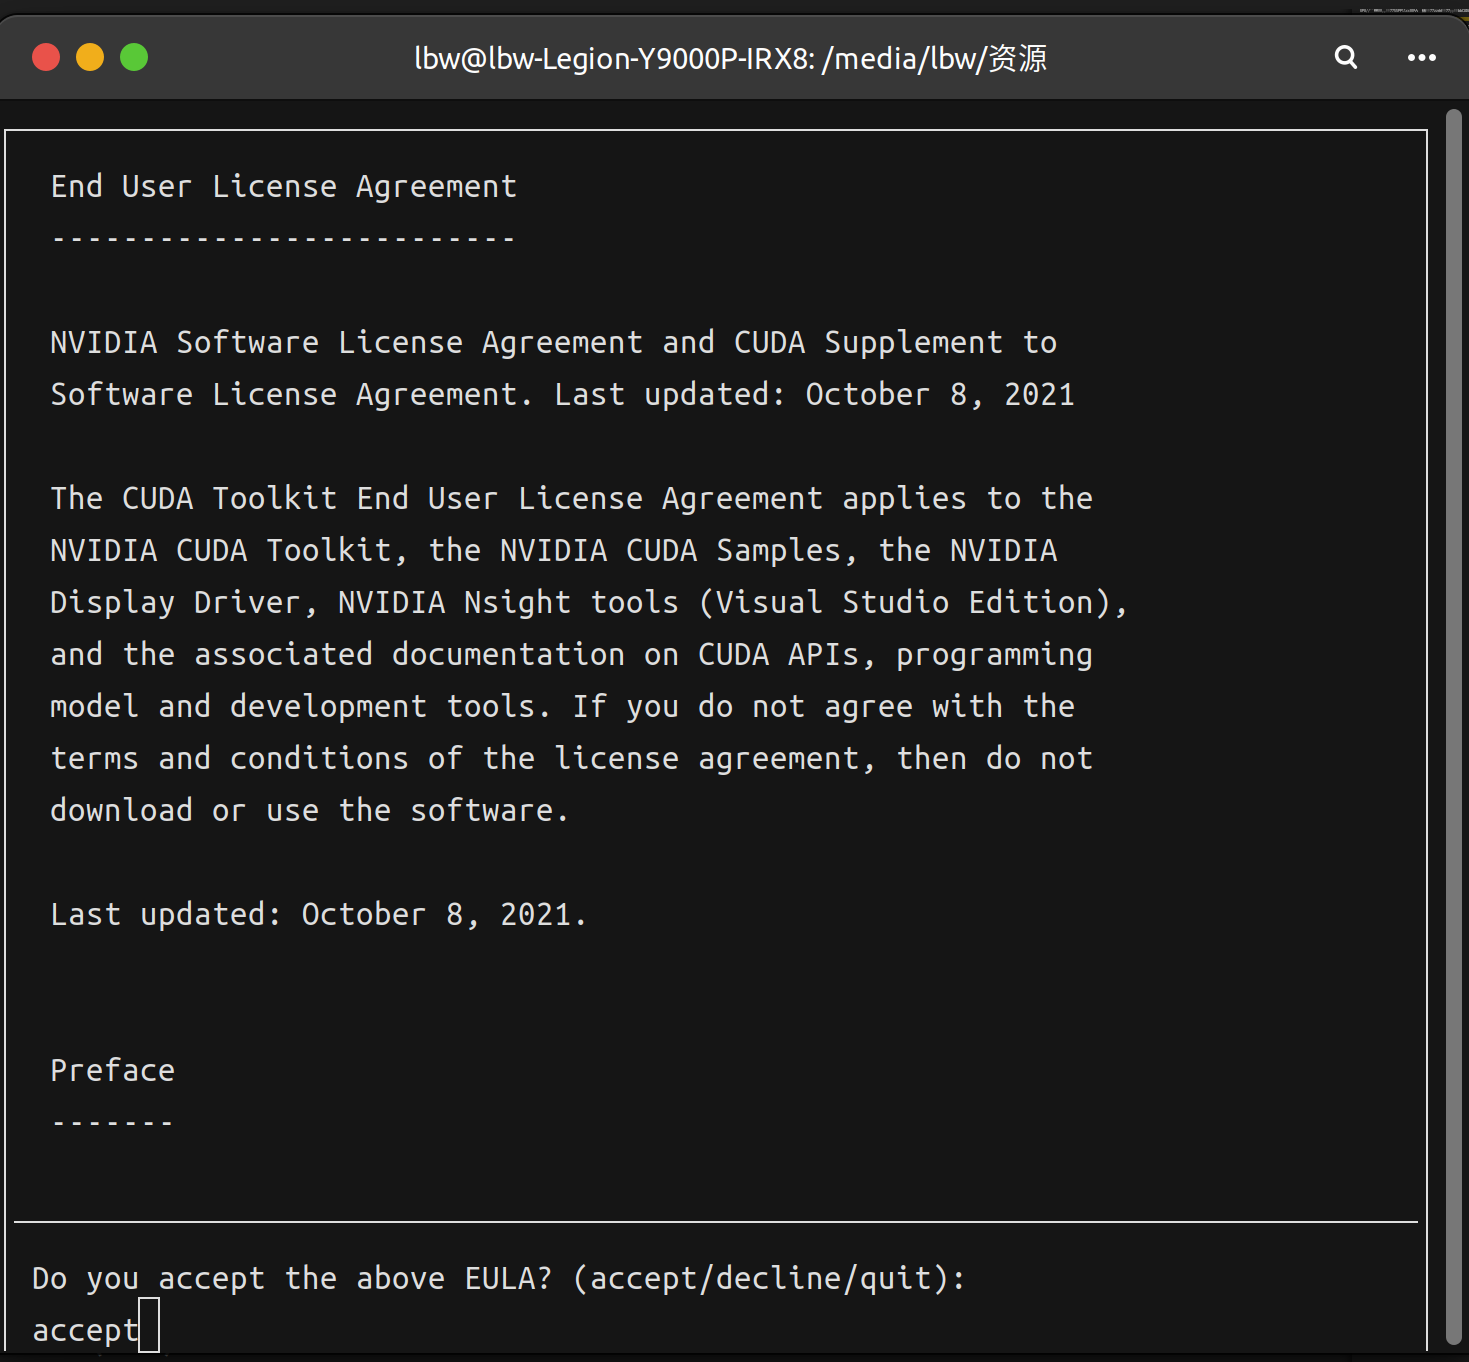
\includegraphics[width=0.7\textwidth]{CUDA_accept.png}
    \caption{接受许可}
    \label{fig:cuda_install2}
\end{figure}

\begin{figure}[H]
    \centering
    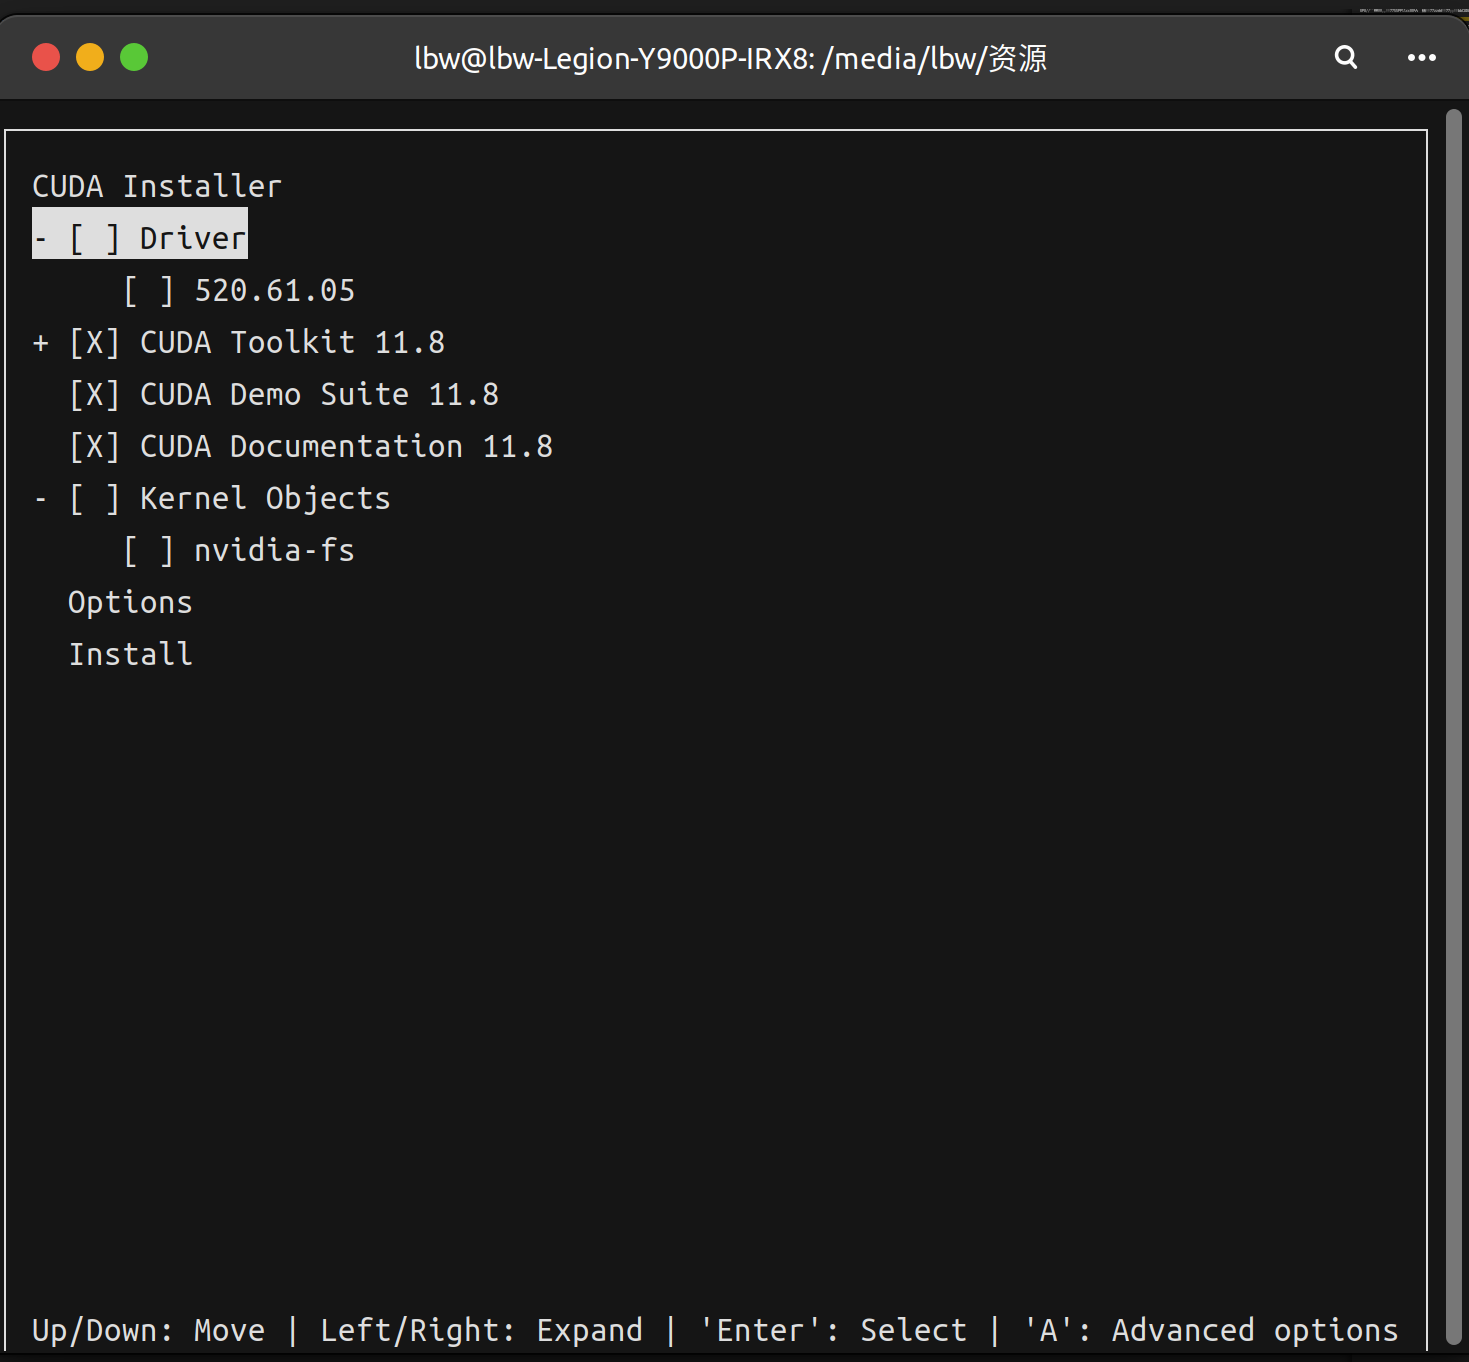
\includegraphics[width=0.7\textwidth]{CUDA_warning.png}
    \caption{组件选择：务必取消 Driver}
    \label{fig:cuda_install3}
\end{figure}

\textbf{关键：}若系统已有可用 NVIDIA 驱动，安装 Toolkit 时应用空格键\textbf{取消勾选 Driver}，只装 toolkit。
否则可能覆盖驱动导致黑屏。

按提示配置环境变量，例如：
\begin{tbash}
export PATH=/usr/local/cuda/bin:$PATH
export LD_LIBRARY_PATH=/usr/local/cuda/lib64:$LD_LIBRARY_PATH
\end{tbash}
写入 \texttt{\textasciitilde/.bashrc} 后 \texttt{source}。验证：
\begin{tbash}
nvcc --version
\end{tbash}

\begin{figure}[H]
    \centering
    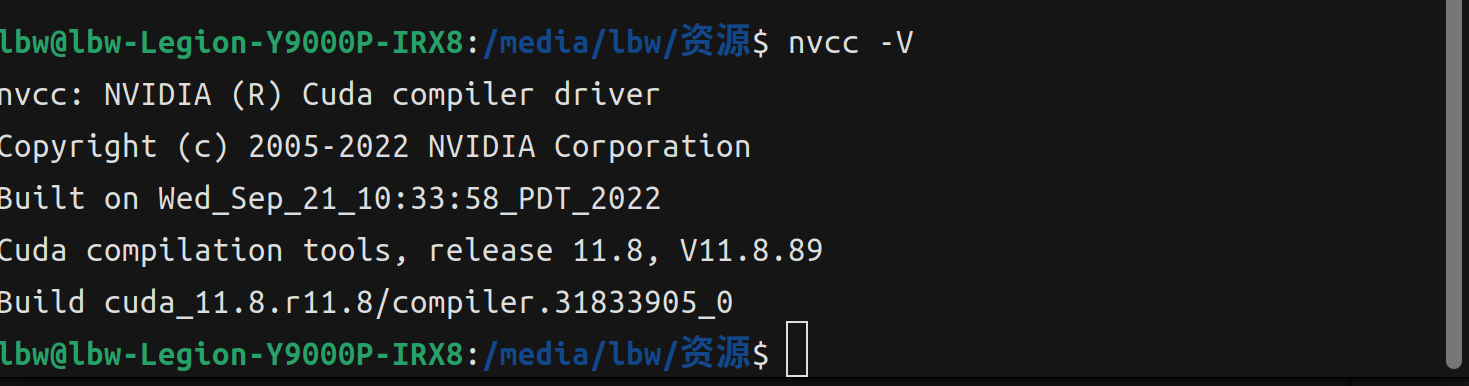
\includegraphics[width=0.7\textwidth]{CUDA_check.png}
    \caption{nvcc 版本输出示例}
    \label{fig:cuda_check}
\end{figure}

亦可用发行版包管理或 NVIDIA 官方 apt 源安装，原理相同：驱动与 toolkit 版本兼容即可。

\subsection{安装 cuDNN*}

cuDNN 是面向深度网络的加速库。需与 CUDA 主版本匹配，从 NVIDIA 开发者站点下载对应包后解压拷贝：
\begin{tbash}
tar -xzvf cudnn-*-linux-x64-*.tgz
sudo cp cuda/include/cudnn*.h /usr/local/cuda/include
sudo cp cuda/lib64/libcudnn* /usr/local/cuda/lib64
sudo chmod a+r /usr/local/cuda/include/cudnn*.h /usr/local/cuda/lib64/libcudnn*
\end{tbash}
训练框架（如带 GPU 的 PyTorch）通常自带或通过 pip/conda 拉取匹配的运行时；
手写调用 cuDNN API 时才必须显式安装开发文件。

\section{异构计算：Host 与 Device}

GPU 一般不独立运行完整操作系统任务，而是作为 CPU 的协处理器。
CPU 端称为 \textbf{host}，GPU 端称为 \textbf{device}，二者经 PCIe 等总线连接。
典型流程：
\begin{enumerate}
    \item Host 分配设备内存（\texttt{cudaMalloc}）；
    \item 将数据从 Host 拷到 Device（\texttt{cudaMemcpy}）；
    \item 启动 kernel 在 GPU 上计算；
    \item 将结果拷回 Host（\texttt{cudaMemcpy}）；
    \item 释放设备内存（\texttt{cudaFree}）。
\end{enumerate}

\begin{figure}[H]
    \centering
    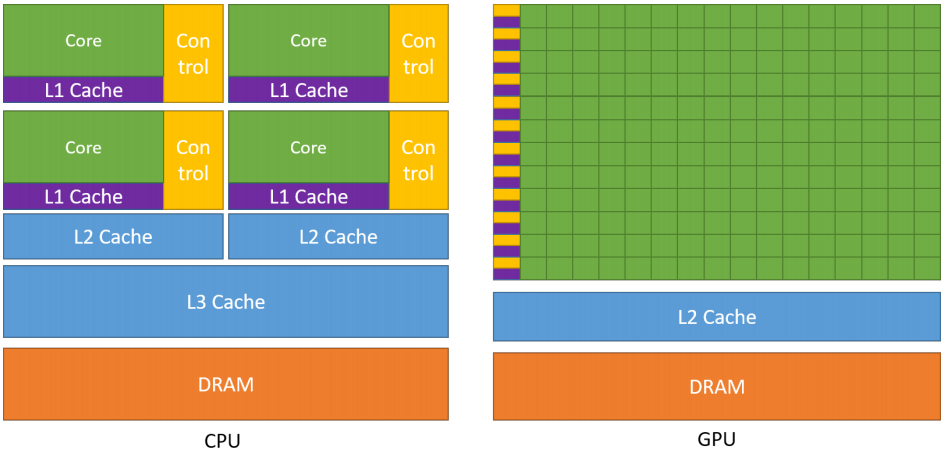
\includegraphics[width=0.85\textwidth]{Host-Device.png}
    \caption{CPU--GPU 异构架构示意}
    \label{fig:host_device}
\end{figure}

数据搬运开销不可忽视：若计算量很小而拷贝很重，整体可能比纯 CPU 更慢。
工程上应尽量减少往返拷贝，或把多步处理串在 Device 侧完成。

\section{CUDA 编程基础}

以下内容依据 NVIDIA \emph{CUDA Programming Guide} 中 Intro / Writing Kernels 章节整理。

\subsection{线程层次：Thread、Block、Grid}

Kernel 启动时创建大量线程，组织为：
\begin{itemize}
    \item \textbf{Thread}：执行同一段 kernel 代码的基本单位，通过内置变量区分各自数据；
    \item \textbf{Block}：一组可协作的线程，共享一块 \textbf{shared memory}，可用 \texttt{\_\_syncthreads()} 同步；
    \item \textbf{Grid}：若干 Block 的集合，分布在多个 SM（Streaming Multiprocessor）上执行。
\end{itemize}

核内常用内置变量：\texttt{threadIdx}、\texttt{blockIdx}、\texttt{blockDim}、\texttt{gridDim}（可达三维）。
一维全局下标常写为：
\begin{tcode}
int i = blockIdx.x * blockDim.x + threadIdx.x;
\end{tcode}

启动语法（triple chevron）：
\begin{tcode}
kernel<<<gridDim, blockDim>>>(args...);
// 或 dim3 grid(gx, gy); dim3 block(bx, by);
// kernel<<<grid, block>>>(...);
\end{tcode}
第一参数为 Grid 维度，第二参数为每个 Block 的线程数。
Block 大小常取 128、256 等，需结合占用率与问题规模调试。

\subsection{第一个例子：向量加法}

\begin{tcode}
#include <cuda_runtime.h>
#include <cstdio>

__global__ void vecAdd(const float* A, const float* B, float* C, int n) {
    int i = blockIdx.x * blockDim.x + threadIdx.x;
    if (i < n) C[i] = A[i] + B[i];
}

int main() {
    const int n = 1 << 20;
    size_t bytes = n * sizeof(float);
    float *hA = new float[n], *hB = new float[n], *hC = new float[n];
    for (int i = 0; i < n; ++i) { hA[i] = 1.f; hB[i] = 2.f; }

    float *dA, *dB, *dC;
    cudaMalloc(&dA, bytes); cudaMalloc(&dB, bytes); cudaMalloc(&dC, bytes);
    cudaMemcpy(dA, hA, bytes, cudaMemcpyHostToDevice);
    cudaMemcpy(dB, hB, bytes, cudaMemcpyHostToDevice);

    int threads = 256;
    int blocks = (n + threads - 1) / threads;
    vecAdd<<<blocks, threads>>>(dA, dB, dC, n);
    cudaDeviceSynchronize();

    cudaMemcpy(hC, dC, bytes, cudaMemcpyDeviceToHost);
    printf("C[0]=%f\n", hC[0]); // 期望 3

    cudaFree(dA); cudaFree(dB); cudaFree(dC);
    delete[] hA; delete[] hB; delete[] hC;
    return 0;
}
\end{tcode}

要点：
\begin{itemize}
    \item 设备端函数用 \texttt{\_\_global\_\_} 修饰，由 Host 启动；
    \item 必须用 \texttt{if (i < n)} 防止越界（末尾 Block 可能超出）；
    \item \texttt{cudaMemcpy} 最后一参指明方向：\texttt{HostToDevice} / \texttt{DeviceToHost} / \texttt{DeviceToDevice}。
\end{itemize}

编译示例：
\begin{tbash}
nvcc -O2 vec_add.cu -o vec_add
./vec_add
\end{tbash}

\subsection{内存层次（入门）}

\begin{itemize}
    \item \textbf{Global memory}：容量大、延迟高，\texttt{cudaMalloc} 得到的指针通常指向此处；
    \item \textbf{Shared memory}：Block 内共享的片上暂存，延迟低、容量小，适合复用数据；
    \item \textbf{Registers / Local}：每线程私有；寄存器溢出时可能落到 local memory。
\end{itemize}

Shared memory 示例骨架：
\begin{tcode}
__global__ void demo(float* out, const float* in) {
    __shared__ float tile[256];
    int tid = threadIdx.x;
    int i = blockIdx.x * blockDim.x + tid;
    tile[tid] = in[i];
    __syncthreads(); // 等待块内全部写完再读
    out[i] = tile[tid]; // 示意：实际可做归约、卷积滑窗等
}
\end{tcode}
块内协作读写前务必 \texttt{\_\_syncthreads()}，否则存在数据竞争。

\subsection{错误检查习惯}

生产代码应对每次 CUDA API 检查返回值，例如：
\begin{tcode}
#define CUDA_CHECK(call) do { \
  cudaError_t e = (call); \
  if (e != cudaSuccess) { \
    fprintf(stderr, "CUDA error %s:%d: %s\n", __FILE__, __LINE__, \
            cudaGetErrorString(e)); \
    exit(1); \
  } \
} while(0)
\end{tcode}
Kernel 启动为异步，常用 \texttt{cudaGetLastError()} 与 \texttt{cudaDeviceSynchronize()} 捕获启动/执行错误。

\subsection{与 CMake 集成}

现代 CMake（3.18+）推荐启用 CUDA 语言并链接 Toolkit 目标：
\begin{tcode}
cmake_minimum_required(VERSION 3.18)
project(cuda_demo LANGUAGES CXX CUDA)
find_package(CUDAToolkit REQUIRED)
add_executable(vec_add vec_add.cu)
target_link_libraries(vec_add PRIVATE CUDA::cudart)
\end{tcode}

\section{从算子到推理部署*}

手写 kernel 适合学习与关键热点优化；多数视觉推理优先走成熟栈：
\begin{enumerate}
    \item 训练框架导出 \textbf{ONNX}（跨框架中间表示）；
    \item 用 \textbf{TensorRT}（或 OpenVINO 等）构建优化引擎（融合算子、精度校准等）；
    \item 在线加载 \texttt{.engine} 做低延迟推理。
\end{enumerate}
TensorRT 依赖 CUDA；引擎往往与具体 GPU 架构相关，换卡常需重建。
深度学习章中的部署小节与此衔接：本卷强调 CUDA 是 GPU 路径的底座，
具体 TensorRT API 可在项目仓库与 NVIDIA 文档中深入。

\section{常见问题与边界}

\begin{itemize}
    \item 笔记本双显卡：确认进程跑在 NVIDIA 独显上（\texttt{nvidia-smi} 看进程）。
    \item WSL / 容器：需额外配置 GPU 透传，与裸机步骤不同。
    \item 无 GPU 环境：可学概念与写可在 CPU 回退的代码路径；本章验收中的运行项需有可用设备。
\end{itemize}

延伸阅读：
\url{https://docs.nvidia.com/cuda/cuda-programming-guide/02-basics/intro-to-cuda-cpp.html}。


\section{本章小结}
CPU 主机负责组织任务，GPU 设备负责并行计算。驱动负责访问设备，Toolkit 提供编译工具和开发库；版本信息要分开检查。应熟练计算网格索引、检查越界、核对每次 API 返回值，并计入拷贝与同步开销。共享内存和推理引擎属于后续优化入口，先保证输出正确。

\begin{problemset}
\item 基础：阈值化每个像素与按前一元素结果递推，哪一个更容易直接映射为独立线程？
\item 基础：nvidia-smi 正常但 nvcc 不存在，能否断定驱动未安装？
\item 基础：两个长度 512 的 float 输入和一个输出，一次流程需拷贝多少字节？
\item 基础：n=513、每块 256 线程，需要多少块？最后有多少线程必须跳过访问？
\item 基础：Shared memory 的共享范围是什么？部分线程在屏障之前返回有什么风险？
\item 提高：kernel 已成功提交，程序是否就一定计算成功？如何捕获执行错误？
\item 实践：有可用 GPU 时分别记录 nvidia-smi 与 nvcc 的版本；无 GPU 时分析教师提供的这两段输出，说明各自代表什么。
\end{problemset}

\section{本章验收}
\begin{enumerate}
    \item 展示现有驱动与 Toolkit 状态，解释安装向导中 Driver 选项的处理依据。
    \item 用 nvcc 或 CMake 编译向量加法，对检查者给出的非整块长度验证全部结果，并展示错误检查位置。
    \item 测量包含数据传输的完整流程耗时；选做在固定块大小下改写共享内存示例并验证边界长度。
\end{enumerate}


% ============================================================
\chapter{相机与成像原理}

\begin{introduction}
  \item 学习目标：计算曝光与运动模糊；区分像素格式与噪声；验证标定模型；使用 ROS2 标定包并部署校正图像。
  \item 建议学时：约 4--6 天，含标定采集与部署实验。
  \item 本卷边界：本章聚焦成像与标定实验；实车选型和曝光检查表见卷三，投影与 PnP 推导见本卷几何视觉章。
\end{introduction}

\section{成像参数与标定}

\subsubsection{先把相机参数认清楚}
前面我们已经能读图、跑模型，还能让 GPU 做点工作了。不过算法接到相机以后，常常先遇到一个很朴素的问题：图片糊了、亮部白成一片，或者颜色看起来不对。这时候先别忙着换网络，我们得知道图像是怎样形成的。相机参数不是越大越好，先弄清它影响哪一步，调起来才有方向。

\paragraph*{感光元件：CCD 与 CMOS}
感光元件把入射光转换为电荷，再经过读出、放大和模数转换（Analog-to-Digital Conversion，ADC）形成数字数据。电荷耦合器件（Charge-Coupled Device，CCD）通常通过电荷转移集中读出；互补金属氧化物半导体（Complementary Metal-Oxide Semiconductor，CMOS）图像传感器则利用像元、列读出等电路取得信号，可以集成更多处理功能。这里的“互补”指电路工艺，不是两种电荷凑在一起形成图片。

原来常用的 CCD/CMOS 对比能帮你认结构，却不能直接当成产品排名。输出节点数、噪声、速度、功耗和供电都取决于具体设计；现代 CMOS 也有全局快门。我们选运动目标相机时，还要分别查快门类型、工作分辨率、帧率、像元尺寸和曝光范围，不能看见 CMOS 三个字就断言它一定有果冻效应。
\begin{example}[照着官方规格做一张参数卡]
打开 \href{https://docs.baslerweb.com/aca1920-155um}{Basler acA1920-155um 官方规格}，在 General Specifications 查四个字段：全分辨率为 $1936\times1216$，默认模式为 $1920\times1200$，像元为 $5.86\times5.86\,\mu$m，快门为 global shutter。这只是练习查表，没有接入这台相机，也不据此推荐购买。默认模式和传感器完整尺寸不同，后面的标定要用实际输出模式。
\end{example}
\begin{exercise}\label{ex:v2-camera-sensor}
给手边设备做参数卡，记录完整型号、规格来源、工作分辨率、像元尺寸和快门；暂时没有设备就按上述官方页面完成查表，实机确认留作未完成。缺字段写未知，不用 CMOS 名称猜快门。
\end{exercise}

\subsubsection{光圈、曝光与增益：先保住清晰度}
光圈通过入瞳大小控制进光。光圈数（f-number）是焦距与入瞳直径之比，$N=f/D_{\mathrm{pupil}}$；f/4、F4 是常见写法。分母数字越大，孔径反而越小，这个方向刚接触时容易记反。相邻整档的光圈数约差 $\sqrt2$，同样时间内的入光量约差一倍，例如 f/2.8、f/4、f/5.6、f/8。

镜头可能是固定光圈，也可能用多片叶片组成虹膜光圈；历史上的圆盘孔、猫眼式、瞬时光圈和兼快门结构各有用途，名字不用背成考试口诀。拿到工业镜头时，首先确认能否调光圈，再找对光圈环与对焦环，按刻度记录设置，不要把拧对焦环当成改曝光。

快门控制曝光时间。机械快门可以遮光，电子快门则由传感器控制曝光时序，不一定有一块板子在镜头前开合。曝光越长，收到的光通常越多，但运动目标在这段时间内也走得更远。数字相机的 ISO 或工业相机的增益（gain）改变信号放大与输出亮度，不能让传感器凭空收到更多光子；增益也可能放大噪声、减少高光余量。工业相机常用 dB，不能把数值直接当 ISO。
\begin{example}[暗了以后怎样调]
光照和增益不变时，从 f/4 改为 f/2.8 约增加一档入光量，原来的 2 ms 可近似缩为 1 ms，保持相近亮度。从 f/4 收到 f/5.6 则相反，精算时间比例为 $(5.6/4)^2=1.96$。这还没有计入透过率和自动处理，不要求实际灰度恰好翻倍。实拍前关闭会自动改曝光/增益的设置，核对驱动的时间单位，拍同一运动目标并保存配置与图片，再判断亮度和清晰度。
\end{example}
\begin{exercise}\label{ex:v2-camera-exposure}
从 f/4 收到 f/5.6，保持光照、增益和亮度，原来 1 ms 应改为多少？随后在实机分别改变曝光与增益，解释模糊、亮度和噪声；没有设备时保留实拍缺口。
\end{exercise}

\subsubsection{卷帘与全局：模糊和形变不是一回事}
卷帘快门（rolling shutter）让不同图像行在不同时刻开始曝光。物体在这些时刻的位置不同，拼成一帧就可能歪斜，这就是常说的果冻效应。其程度与运动、读出方向以及首末行时差有关；只看分辨率或标称帧率，不能直接算出整帧读出时间。

全局快门（global shutter）让全部像元在同一时间区间曝光，之后再按设计读出，能避免这种逐行时差造成的形变。不过它仍然要积累一段时间的光；曝光过长，运动物体照样糊。全局不是“瞬间冻结一切”的魔法按钮。
\begin{figure}[H]
\centering
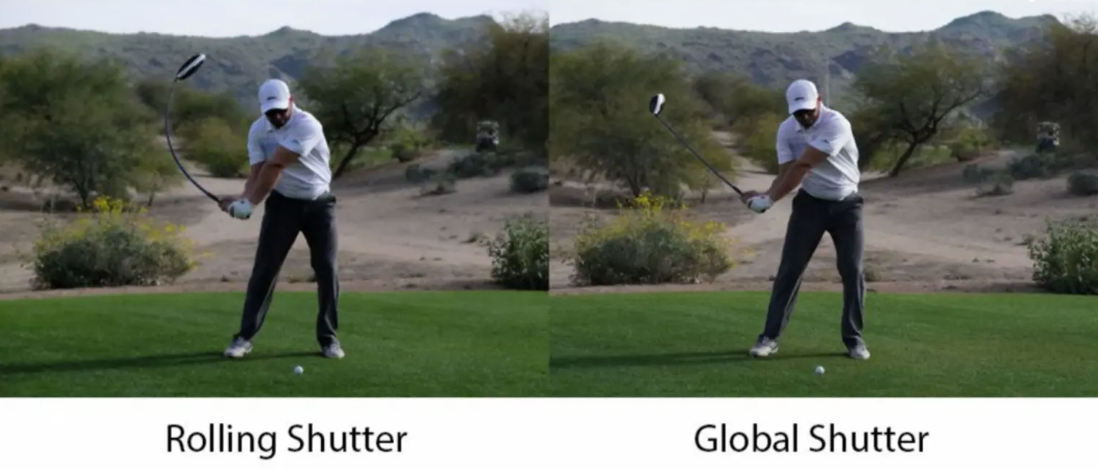
\includegraphics[width=0.82\textwidth]{images/rolling_shutter_revised.png}
\caption{原教材的快门对比示意：看球杆形状，不把照片当本次受控实拍}
\label{fig:v2-camera-shutter-photo}
\end{figure}
\begin{example}[把时序写成数值]
设图像速度为 800 pixel/s，单行曝光 2 ms，则曝光内位移约为 1.6 pixel；如果首末行曝光起点另外相差 6 ms，跨行对应的位置差约为 4.8 pixel。这两个量描述不同现象，缩短曝光不保证同时缩短读出时差。我们将在下面的 optics 中计算曝光位移，在“运动预算”练习中一起核对读出差。
\end{example}
\begin{conclusion}
传感器类型说明读出结构，快门类型说明曝光时序。光圈改变入光，曝光决定积分时间，增益放大已有信号。选运动相机先核对实际快门与读出条件；静态场景可以权衡分辨率和成本，不给所有卷帘产品套同一条结论。
\end{conclusion}

\subsubsection{准备一个可以反复检查的小实验}
本章完整项目在本卷 \path{examples/camera/calibration-lab-demo}。我们先用小数组算成像参数，再生成明确的模拟棋盘格，接着检测、标定、验证，最后接到 ROS 的保存和校正链路。模拟实验能排查单位与接口，却不能代替曝光、焦点和硬件同步的实拍验收。
\begin{example}[安装依赖并进入项目]
在 Ubuntu 22.04 / Humble 环境里使用系统 Python，避免把另一个虚拟环境的 cv2 混进 ROS。普通数值部分需要 NumPy、OpenCV 和 PyYAML；图形标定稍后再安装 ROS 包。
\begin{tbash}
sudo apt install python3-numpy python3-opencv python3-yaml
cd /你的教材目录/02-专项技术栈/examples/camera/calibration-lab-demo
python3 -c "import cv2,numpy,yaml; print(cv2.__version__,numpy.__version__)"
\end{tbash}
把路径换成实际位置，后面的短命令都从这个项目目录执行。记录命令输出的 OpenCV 和 NumPy 版本，后续实验使用同一个系统解释器。目录如下，输出放到 data/out，不覆盖教材源文件：
\begin{tbash}
calibration-lab-demo/
  optics.py            # 曝光、景深和单位计算
  format_gamma.py      # Bayer 与 Gamma 小数组
  noise.py             # 声明模型的加噪实验
  board.py             # 统一板规格与检测
  generate.py          # 已知几何模型的模拟图
  model_io.py          # 标定 YAML 保存与读取
  calibrate.py         # 多图标定与逐图误差
  validate.py          # 固定内参的独立图检查
  replay_ros.py        # 回放、参数服务和持久保存
  check_ros.py         # 原图/参数/校正输出核对
  stereo.py            # 双目几何与极线残差
  README.md
\end{tbash}
项目准备与命令实践由后面的噪声、格式和标定练习一起检查，不再出一题重复进入目录。
\end{example}

\subsubsection{噪声：别把“看着有颗粒”当成诊断}
图像噪点可能来自光子统计、读出电路、温度、坏点或传输/解码问题。高斯噪声（Gaussian noise）描述幅值分布；白噪声（white noise）描述相关性或频谱条件，两者不是同一个词换语言。读出噪声有时近似高斯，但不能凭图片外观确认全部来源。

泊松噪声（Poisson noise）可描述光子计数的散粒噪声。期望光子数为 $N$ 时，标准差约为 $\sqrt N$，相对标准差为 $1/\sqrt N$。从 100 增加到 400，绝对标准差从 10 变 20，相对噪声却从 10\% 降为 5\%。补光增加光子，增益放大已有值，它们不是等价操作。

乘性噪声可写成 $I'=I(1+\eta)$，扰动幅度随信号变化，这只是建模方式，不说明所有相机噪声都来自信道。椒盐噪声（salt-and-pepper noise）把一部分像素改到极低或极高；出现亮暗点还应查坏点和链路，不能先套滤波再宣布原因找到了。
\begin{figure}[H]
\centering
\begin{minipage}{0.30\textwidth}\centering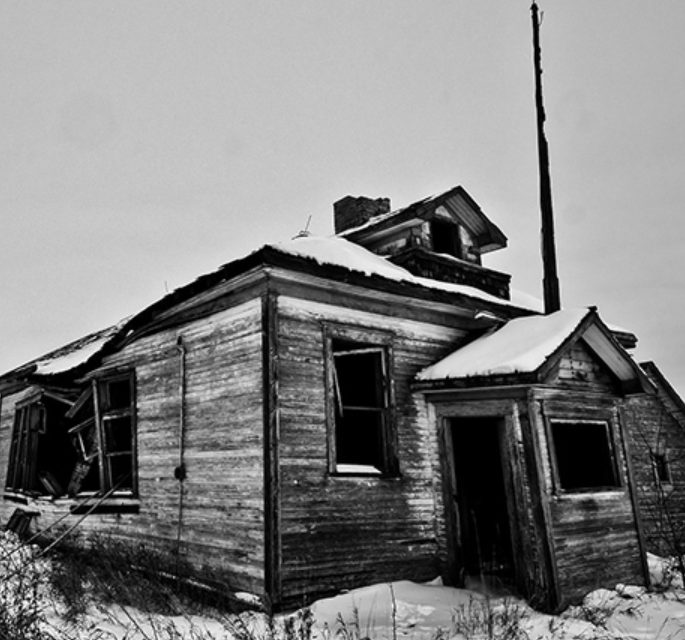
\includegraphics[width=\linewidth]{images/raw_revised.png}\\原图\end{minipage}\hfill
\begin{minipage}{0.30\textwidth}\centering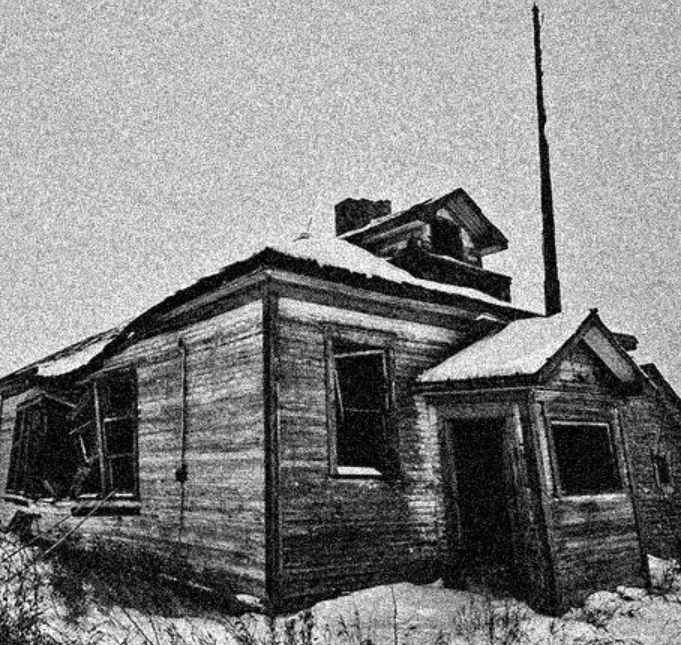
\includegraphics[width=\linewidth]{images/gaussian_revised.png}\\高斯示意\end{minipage}\hfill
\begin{minipage}{0.30\textwidth}\centering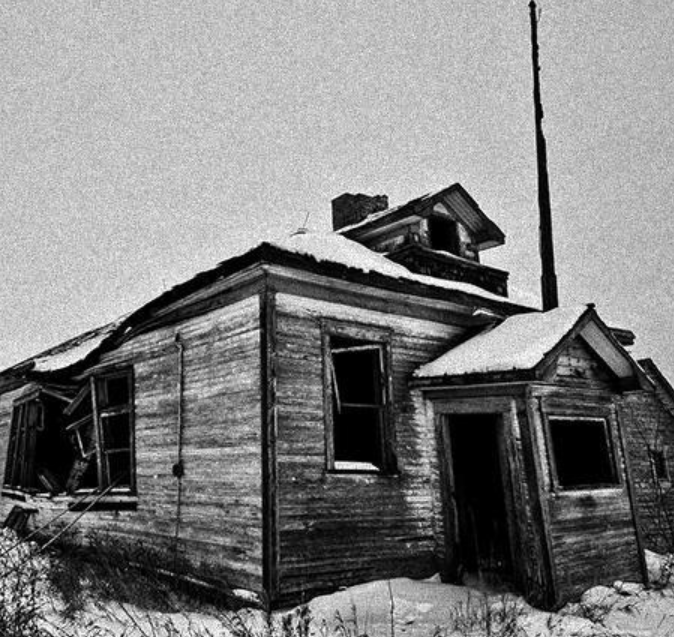
\includegraphics[width=\linewidth]{images/poisson_revised.png}\\泊松示意\end{minipage}

\smallskip
\begin{minipage}{0.30\textwidth}\centering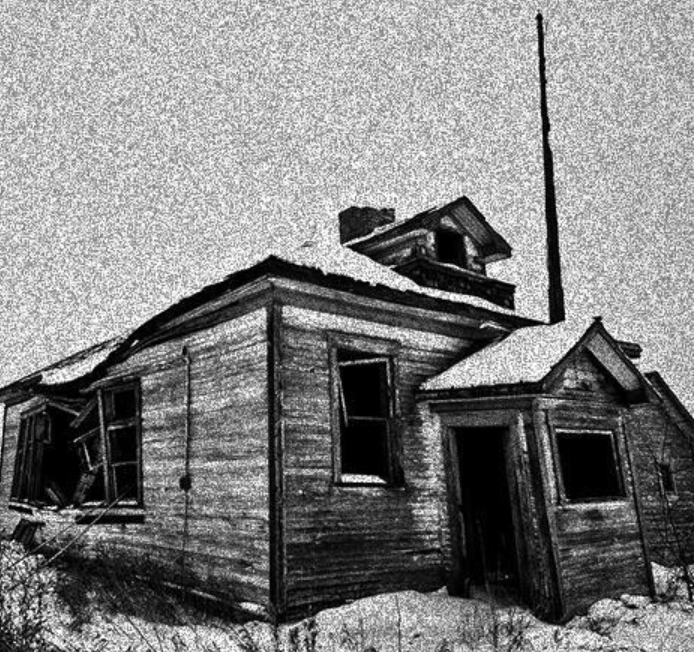
\includegraphics[width=\linewidth]{images/camera_multiplicative_revised.png}\\乘性示意\end{minipage}\hspace{0.06\textwidth}
\begin{minipage}{0.30\textwidth}\centering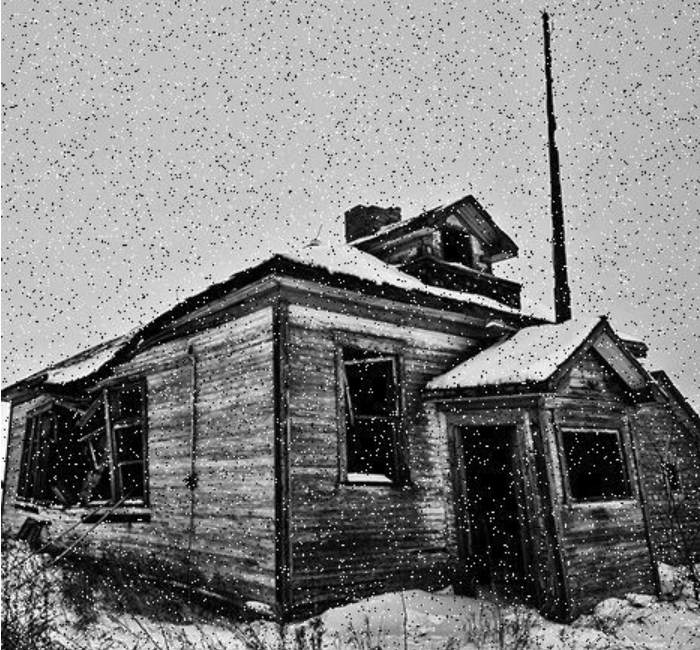
\includegraphics[width=\linewidth]{images/salt_revised.png}\\椒盐示意\end{minipage}
\caption{保留原教材五幅对照图；具体生成参数未知，不据它们倒推传感器噪声}
\label{fig:v2-camera-old-noise}
\end{figure}
\begin{example}[有参数的噪声实验]
noise 抽样 100000 次光子计数，再给同一灰度坡道加四种声明的噪声；随机种子固定，输出截到 0–255 并保存。坡道用于检查输入，不是相机实测。
\end{example}
\lstinputlisting[numbers=left,language=Python,basicstyle=\footnotesize\ttfamily,caption={noise.py}]{examples/camera/calibration-lab-demo/noise.py}
\begin{tbash}
python3 noise.py --photons 900 --output out/noise
\end{tbash}
通用形式是 \texttt{python3 noise.py [选项]}，photons 为期望光子数，output 为输出目录。本次理论标准差 30、相对值约 0.0333，抽样标准差约 30.015；不要求随机实验的小数等于理论值。滤波选择见 OpenCV 章，光照和读出问题仍需设备排查。
\begin{exercise}\label{ex:v2-camera-noise}
手算 N=900 的标准差和相对噪声，再运行 --photons 100 与 400。解释绝对噪声变大为何仍可能改善相对噪声，指出补光与增益的不同。
\end{exercise}

\subsubsection{像素格式与 Gamma：形状对了，颜色也要对}
彩色 Bayer 阵列每个位置只采一种颜色，典型 $2\times2$ 单元有两个 G、一个 R、一个 B；原始数据是单通道采样。不同起点形成 RGGB/BGGR 等排列，去马赛克（demosaicing）后才得到每像素三通道。Bayer 不是“.raw 后缀”的同义词，RAW 容器也可能有头部、位打包、黑电平和元数据。

RGB 每像素有红绿蓝三通道，OpenCV 常用 BGR 顺序。无填充的 640×480、8 位样本，Bayer8 为 307200 字节，RGB8 为 921600；10/12 位打包、行填充和 JPEG 压缩不能直接套这两个数。ROS 中还需核对 encoding、step 和 data 长度，前面的图像桥接章已有完整实验。

Gamma 是非线性亮度映射。本例约定 $y=x^{1/\gamma}$，$x=I/255$；gamma=2.2 提亮暗部，gamma=1 不变，小于 1 则压暗。另一些相机参数直接用指数，方向可能相反，先查文档。它不会恢复已经过曝或量化丢掉的细节，简单幂律也不等于完整 sRGB 编码。
\begin{example}[核对 Bayer 与查找表]
程序先造 8×6 RGGB：R=200、G=100、B=50，用 OpenCV 4.5 的 \texttt{COLOR\_BayerBG2BGR} 核对中心；这个两字母名称对应本例的 RGGB 排列，不能只看名字猜通道顺序。随后建立 256 项查找表（Look-Up Table，LUT），用 cv2.LUT 处理坡道。构表只做 256 次幂运算，不对每帧每像素重复求幂。
\end{example}
\lstinputlisting[numbers=left,language=Python,basicstyle=\footnotesize\ttfamily,caption={format\_gamma.py}]{examples/camera/calibration-lab-demo/format_gamma.py}
\begin{tbash}
python3 format_gamma.py --gamma 2.2 --output out/format
python3 format_gamma.py --gamma 1 --output out/identity
\end{tbash}
预期 Bayer 为 48 字节、BGR 为 144，中心 [50,100,200]；2.2 时 LUT[128]=186，1 时 identity=true。换阵列起点却不换代码，颜色就可能反了，形状正确也救不了。
\begin{figure}[H]
\centering
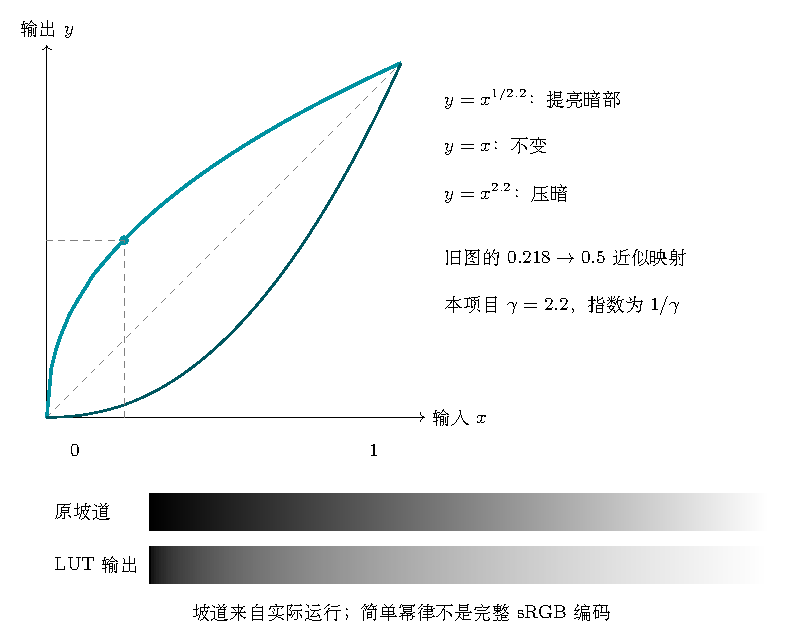
\includegraphics[width=0.94\textwidth]{images/camera_gamma_revised.pdf}
\caption{两种指数约定要分清；坡道使用本项目实际 LUT 输出}
\label{fig:v2-camera-gamma}
\end{figure}
\begin{exercise}\label{ex:v2-camera-format}
计算 1280×720 的 Bayer8/BGR8 字节，不计填充。解释 RGB/BGR 与 Bayer 排列是两种不同约定，说明文件大小为何可能不同。
\end{exercise}
\begin{exercise}\label{ex:v2-camera-gamma}
运行 gamma=1 核对完整坡道，再改为 0.5。说明暗部变化方向，以及为什么提亮饱和像素不能找回纹理。
\end{exercise}

\subsubsection{景深与焦段：不是“对过焦就一直清楚”}
对普通薄透镜近似，只有一个物平面严格合焦；离开它的点在像平面形成弥散圆（circle of confusion）。模糊在当前清晰度判据内，看起来仍够清楚，这段物方范围叫景深（depth of field）。像方允许的范围叫焦深（depth of focus），不要互换。容许弥散圆 $c$ 由成像、观察/检测要求等决定，不是所有系统都固定等于一个像元。
\begin{figure}[H]
\centering
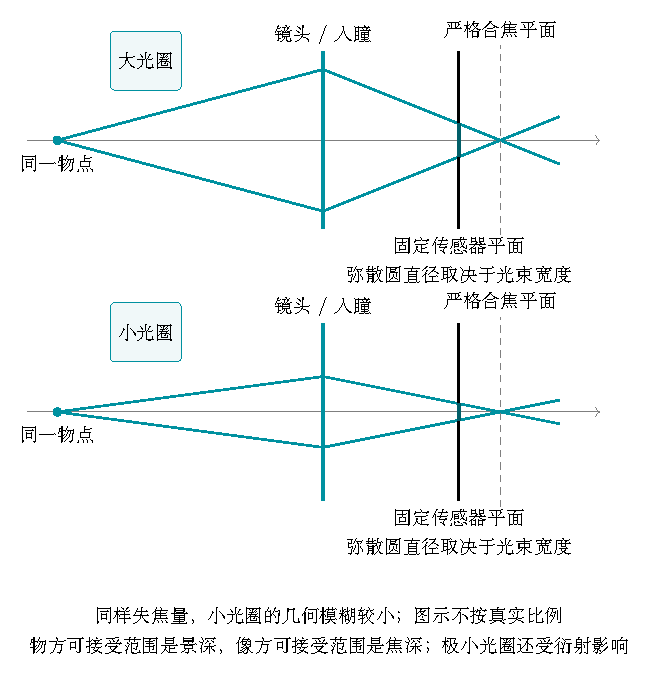
\includegraphics[width=0.94\textwidth]{images/camera_focus_revised.pdf}
\caption{合焦、可接受模糊与失焦；示意不按真实尺寸绘制}
\label{fig:v2-camera-focus}
\end{figure}
同样焦距、对焦距离和判据下，收小光圈通常增大几何景深，却也减少进光，极小光圈还受衍射影响。其他条件不变时，更长焦距通常让景深更浅，距离增大通常让景深更大；改变成像倍率或裁剪后，别只背结论就跳过条件。

\paragraph*{景深估算*}
沿用旧图的薄透镜关系，焦距 $f$、光圈数 $N$、弥散圆 $c$、物距 $s$ 采用相同长度单位，设 $h=f^2/(Nc)$，超焦距为 $H=h+f$。近、远界为
\[
s_{\mathrm{near}}=\frac{hs}{h+s-f},\qquad
s_{\mathrm{far}}=\frac{hs}{h-s+f}.
\]
远界分母不为正时取无穷，不输出负距离。前景深为 $s-s_{\mathrm{near}}$，后景深为 $s_{\mathrm{far}}-s$；有限远界下，后者通常较大。图 \ref{fig:v2-camera-dof} 保留旧图总景深与远距离近似；程序不模拟多片镜头和衍射。
\begin{figure}[H]
\centering
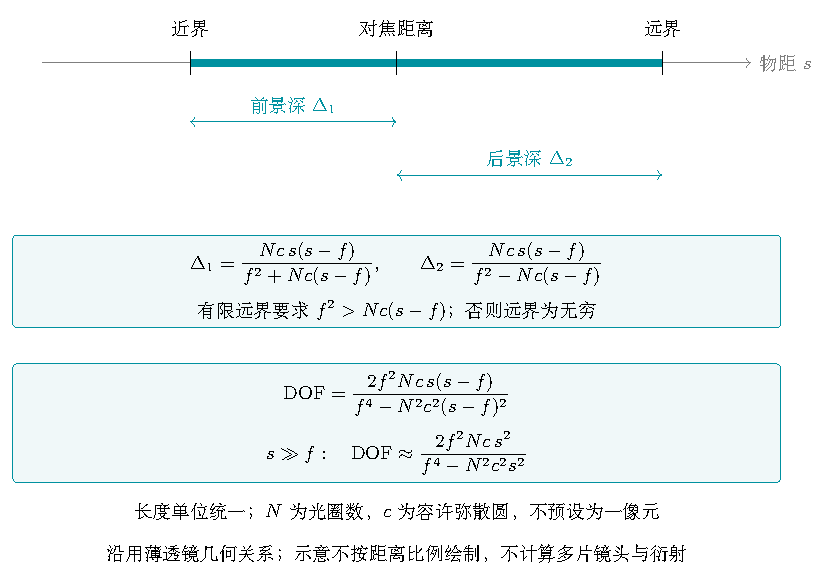
\includegraphics[width=0.94\textwidth]{images/camera_dof_revised.pdf}
\caption{前后景深、总景深与近似的条件}
\label{fig:v2-camera-dof}
\end{figure}
\begin{example}[把单位和边界写进程序]
optics 固定毫米、毫秒和 pixel/s，拒收非正/非有限参数；超过超焦距时 far=null 表示无穷。它还汇总后面运动、裁剪、双目和同步的手算值，覆盖小规模计算，不模拟硬件。
\end{example}
\lstinputlisting[numbers=left,language=Python,basicstyle=\footnotesize\ttfamily,caption={optics.py}]{examples/camera/calibration-lab-demo/optics.py}
\begin{tbash}
python3 optics.py
python3 optics.py --aperture 8
\end{tbash}
默认 $f=16$ mm、$N=4$、$c=0.01$ mm、$s=2000$ mm，H=6416 mm，近界约 1526.72、远界约 2898.55 mm；N=8 时 H=3216。实际清晰度仍需拍图确认。
\begin{exercise}\label{ex:v2-camera-dof}
运行 N=8 记录超焦距和近远界，再设 --distance 7000。解释 far=null，为什么不能说收小光圈在任何情况下都改善成像。
\end{exercise}

\subsubsection{运动预算与焦段选择}
现在把“不能太糊”变成一个数。图像速度近似恒定时，曝光位移 $b=vt$；最多容许 $b_{\max}$，则 $t\le b_{\max}/v$。$v$ 是 pixel/s，换成世界中的 m/s 还需要成像几何，不能直接混用。
\begin{example}[先算最长曝光，再在相机确认]
\begin{tbash}
python3 optics.py --speed 800 --exposure 2 --budget 1
python3 optics.py --speed 1200 --exposure 2 --budget 0.6
\end{tbash}
第一条位移 1.6 pixel、最长曝光 1.25 ms；第二条最长 0.5 ms。驱动范围、步长、触发与帧周期可能限制设置，填完还要读回并实拍。增益不改变同一曝光内的位移，只可能在亮度允许时帮助采用更短曝光。
\end{example}
\begin{exercise}\label{ex:v2-camera-motion}
手算 800 pixel/s、最多 1 pixel 的最长曝光，与输出核对。另算首末行差 6 ms 时的位置差，说明短曝光与短读出时间各自解决什么。
\end{exercise}

焦距决定视场与目标成像大小。同一传感器、距离和输出模式下，小角度近似中目标宽度与焦距成比例。换长焦能让目标更大，也让视野变窄；先想好最近距离能否看全，再检查接口、对焦、畸变和景深。卷三会接到实车选型，本章先做比例估算。
\begin{example}[从 8 mm 换到 12 mm]
原来宽 20 pixel 的同一目标，约变为 $20\times12/8=30$ pixel，optics 的 width\_8\_to\_12\_px 输出这一值。姿态、距离、像元和裁剪缩放不变才成立；近距离、离轴或畸变明显时重新投影。
\end{example}
\begin{exercise}\label{ex:v2-camera-lens}
估算上述宽度并列出不变条件。若只裁图再放大，为什么不能说相机收到的目标细节也增加了？
\end{exercise}
\begin{conclusion}
先用清晰度预算限制曝光，再用光圈、光照和增益权衡亮度。景深要说明距离与判据，焦段要兼顾像素与视场。格式与 Gamma 改变表达，不能修复曝光模糊、卷帘几何或丢掉的信息。
\end{conclusion}

\subsubsection{从棋盘格照片到内参与畸变}
镜头不是完美针孔，画面边缘直线可能弯曲；标定就是用一组几何参数说明空间点与像素关系。普通针孔用径向/切向畸变，鱼眼常用另一套模型。OpenCV 的 fisheye 四参数不是普通五参数的前四项，不能靠截数组转换。

我们优先用平整棋盘格：9×6 内角点对应 10×7 方格；25 mm 边长在米制程序中是 0.025。板固定在硬板上，实测横纵尺寸，固定工作分辨率、镜头与焦点，再采不同位置、距离和倾角。约 20–30 个有差异姿态可作实拍起点，覆盖不够再补；几百张相似正面图也不能代替倾斜约束。另留验证照片，别全部拿去拟合。
\begin{example}[生成可复现的模拟输入]
board 统一板规格与细化，generate 使用声明的 K/D/姿态渲染理想平面，再按畸变反向采样成原图。种子 2026，越出画面的板跳过，训练与验证按编号分开；front 为正面变体，left/right 为 0.12 m 基线的模拟双目。本次生成 83 张训练、15 张验证、12 张正面和 94 对双目图。truth.json 只记生成条件，标定不读取它。
\end{example}
\lstinputlisting[numbers=left,language=Python,basicstyle=\footnotesize\ttfamily,caption={board.py}]{examples/camera/calibration-lab-demo/board.py}
\lstinputlisting[numbers=left,language=Python,basicstyle=\footnotesize\ttfamily,firstline=1,lastline=37,caption={generate.py：模型与渲染}]{examples/camera/calibration-lab-demo/generate.py}
接着改变位置、距离和倾角，筛去越界图，按组保存；右相机的平移再减基线。所有分组仍是模拟输入，没有加入曝光噪声或传感器读出。
\lstinputlisting[numbers=left,language=Python,basicstyle=\footnotesize\ttfamily,firstline=38,firstnumber=38,caption={generate.py：采样与分组}]{examples/camera/calibration-lab-demo/generate.py}
\begin{tbash}
python3 generate.py --output data
python3 calibrate.py --images data/train --output out
python3 calibrate.py --images data/front --output out/front
\end{tbash}
输出目录的同名图会写入，首次练习用新目录。--images 为输入 PNG 目录，--square 为米制边长，--output 为结果目录。calibrate 检查模式、跳过未检出的板，至少十张有效图才求解；十张只是演示下限，不是合格标准。

这里固定 k3=0，保留 k1/k2/p1/p2，稍后 ROS 命令也明确用两个径向系数，避免不同模型只比 RMS。逐图残差与总 RMS 存 metrics，K/D、尺寸、方格与平移存 NPZ，另写标定 YAML。
\lstinputlisting[numbers=left,language=Python,basicstyle=\footnotesize\ttfamily,caption={calibrate.py}]{examples/camera/calibration-lab-demo/calibrate.py}
本次多姿态 83 张 RMS 约 0.255 pixel，$f_x\approx559.70$；正面 12 张也只有约 0.263 pixel，但 $f_x\approx2493.39$，远离生成的 560。低残差只说明能拟合这些图，不代表内参可信，约束不足不能靠“拍得更多”自动解决。
\begin{exercise}\label{ex:v2-camera-calibrate}
运行 train/front，比较有效数、RMS、K/D 与生成条件，再用各自参数验证 validation/000.png。说明为何不能只按训练 RMS 排名；实拍时保留独立验证和模式记录。
\end{exercise}
\subsubsection{读懂标定结果：模型、采集与误差}
\label{sec:camera-calibration-detail}

相机标定（camera calibration）建立三维点与像素坐标之间的关系。先分清三类量：内参描述相机怎样成像；畸变系数描述镜头偏离理想模型的程度；外参描述两个坐标系的相对位姿。单目标定输出的每张棋盘格位姿，是该次拍摄中“标定板到相机”的变换，不能直接当成“相机到机器人底盘”的固定安装外参。后者需要另做外参或手眼标定。

\paragraph*{从空间点到像素}
令相机坐标系中的点为 $(X_c,Y_c,Z_c)$，且 $Z_c>0$。归一化坐标为 $x=X_c/Z_c$、$y=Y_c/Z_c$。忽略像素轴倾斜时，内参矩阵为
\[
K=\begin{bmatrix}f_x&0&c_x\\0&f_y&c_y\\0&0&1\end{bmatrix},
\qquad u=f_xx+c_x,\quad v=f_yy+c_y.
\]
$f_x,f_y$ 的单位是像素，不是镜头标称的毫米；$c_x,c_y$ 是主点位置，通常接近图像中心，但不应强行当成中心。ROS 光学坐标系通常约定 $x$ 向右、$y$ 向下、$z$ 向前，不能与机器人机体坐标轴混用。

普通针孔模型常使用五个畸变系数 $D=(k_1,k_2,p_1,p_2,k_3)$。令 $r^2=x^2+y^2$，则
\begin{align*}
L&=1+k_1r^2+k_2r^4+k_3r^6,\\
x_d&=xL+2p_1xy+p_2(r^2+2x^2),\\
y_d&=yL+p_1(r^2+2y^2)+2p_2xy.
\end{align*}
再将 $x_d,y_d$ 代入像素公式。三个 $k$ 描述径向变化，两个 $p$ 描述切向变化。其他模型可能使用更多参数；鱼眼模型的四个系数不是上述五参数模型的前四项，不能靠截取数组转换。

\begin{example}[裁剪、缩放后怎样改内参]
假设原图为 $1280\times960$，$f_x=f_y=800$、$(c_x,c_y)=(640,480)$。从左上角 $(100,50)$ 裁取区域，再把裁出的图像按坐标比例缩小到一半。在使用 $u'=s_x(u-u_0)$、$v'=s_y(v-v_0)$ 的坐标约定下：
\begin{tpython}
fx, fy, cx, cy = 800., 800., 640., 480.
u0, v0, sx, sy = 100., 50., 0.5, 0.5
new_K = [[sx*fx, 0., sx*(cx-u0)],
         [0., sy*fy, sy*(cy-v0)], [0., 0., 1.]]
assert new_K == [[400., 0., 270.], [0., 400., 215.], [0., 0., 1.]]
print(new_K)
\end{tpython}
纯图像坐标变换不改变原镜头的归一化畸变模型；但要同步更新尺寸、ROI 和相应投影矩阵。具体缩放实现若采用半像素中心约定，还要按该实现修正主点。切换传感器模式、对焦、变焦或更换镜头并非简单缩放，应重新确认或重新标定。
\end{example}

\paragraph*{怎样采到有效的数据}
平面棋盘格的张正友标定法先利用多视角平面映射约束内参，再联合优化畸变和每张图的位姿。多拍几百张几乎相同的正面图，不等于获得了足够的几何约束。
\begin{enumerate}
\item 将标定板牢固贴在平整硬板上，实测横纵方格边长，检查打印是否被拉伸。9×6 个内角点对应 10×7 个方格；25 mm 在以米为单位的程序中写 0.025。
\item 固定实际工作分辨率、镜头、焦距和对焦位置。关闭会改变几何成像的自动对焦，曝光以角点清晰、黑白区域不过曝为准。
\item 让完整棋盘格出现在中心、四角和边缘，改变距离与俯仰、偏航角；近景覆盖较大面积，远景保留足够清晰的方格。倾斜要有差异，但不能倾斜到角点难以定位。
\item 每个姿态停稳后采集，尤其避免卷帘快门下晃动标定板。先采集约 20--30 个有差异的姿态作为教学起点，再按覆盖和误差补采；张数不是合格证。
\item 另外保留数张清晰、不同位置与倾角的照片作验证，不让它们参与参数拟合。记录相机编号、镜头、分辨率、标定板尺寸和采集日期。
\end{enumerate}

\paragraph*{重投影误差怎样算、怎样看}
把标定板角点用估计的位姿、内参和畸变重新投影到图像，与检测到的角点相减，得到残差。对于总计 $N$ 个二维角点，本章使用
\[
\mathrm{RMS}=\sqrt{\frac{1}{N}\sum_{i=1}^{N}\left\|\hat{\boldsymbol p}_i-\boldsymbol p_i\right\|_2^2}.
\]
单位是像素。不要将所有二维坐标分量的平均误差与这个定义混用，也不要只比较不同分辨率下的数值大小。应同时查看逐图误差、边缘残差、参数合理性、重复标定的稳定性和未参与拟合的图像。某张照片误差很大时先检查模糊、错检或板面弯曲；不能为了降低平均数盲目删除全部边缘照片。

\begin{example}[检查独立照片并生成去畸变图]
先运行前节程序生成 calibration.npz，再保存一张未参与标定的同分辨率照片为 validation.png。以下程序估计该照片中标定板的位姿，保持原 $K,D$ 不变，计算残差并输出 undistorted.png：
\begin{tpython}
import cv2
import numpy as np

data = np.load("calibration.npz")
K, D = data["K"], data["dist"]
img = cv2.imread("validation.png")
if img is None:
    raise ValueError("找不到 validation.png")
size = (img.shape[1], img.shape[0])
if tuple(data["size"]) != size:
    raise ValueError("验证图与标定图分辨率不一致")
gray = cv2.cvtColor(img, cv2.COLOR_BGR2GRAY)
ok, corners = cv2.findChessboardCorners(gray, (9, 6))
if not ok:
    raise ValueError("未找到完整的 9x6 内角点")
criteria = (cv2.TERM_CRITERIA_EPS + cv2.TERM_CRITERIA_MAX_ITER, 30, 0.001)
corners = cv2.cornerSubPix(gray, corners, (11, 11), (-1, -1), criteria)
obj = np.zeros((54, 3), np.float32)
obj[:, :2] = np.mgrid[0:9, 0:6].T.reshape(-1, 2) * 0.025
ok, rvec, tvec = cv2.solvePnP(obj, corners, K, D)
if not ok:
    raise ValueError("位姿求解失败")
pred, _ = cv2.projectPoints(obj, rvec, tvec, K, D)
err = np.linalg.norm(pred.reshape(-1, 2) - corners.reshape(-1, 2), axis=1)
print("验证 RMS / pixel:", np.sqrt(np.mean(err**2)))
print("最大角点残差 / pixel:", err.max())
new_K, roi = cv2.getOptimalNewCameraMatrix(K, D, size, 1.0, size)
out = cv2.undistort(img, K, D, None, new_K)
if not cv2.imwrite("undistorted.png", out):
    raise IOError("无法保存图像")
np.savez("rectified_model.npz", K=new_K, size=size, roi=roi)
\end{tpython}
验证图的位姿仍由该图估计，所以这是固定内参后的泛化检查，并非独立真值精度。检查校正图中直线是否变直、边缘是否过度拉伸；保留全视场时出现黑边可能是正常现象。程序没有裁掉 ROI。后续在该校正图上做 PnP，应使用 new\_K 和零畸变；在原图上做 PnP，则使用原 $K,D$，不要重复去畸变。
\end{example}

\begin{exercise}
原图的 $f_x=1000,c_x=640$，先从左侧裁去 80 pixel，再按本节坐标约定缩小到一半，新的 $f_x,c_x$ 是多少？为什么不能只修改图像宽高？
\end{exercise}

\subsubsection{ROS2 的 camera\_calibration 标定流程}
\label{sec:ros2-camera-calibration}

本节使用 Ubuntu 22.04 / ROS2 Humble。\texttt{camera\_calibration} 属于 image\_pipeline，负责从图像求参数；\texttt{camera\_info\_manager} 是供驱动使用的参数管理库；\texttt{image\_proc} 根据图像和参数生成校正图。安装管理库不会让任意驱动自动具备参数加载服务。

\begin{center}
\begin{tabular}{p{0.31\textwidth}p{0.60\textwidth}}
\toprule[1.5pt]
消息或字段 & 作用 \\
\midrule[1pt]
\nolinkurl{sensor_msgs/msg/Image} & 原始图像及其时间戳、光学坐标系名称。\\
\nolinkurl{sensor_msgs/msg/CameraInfo} & 与该图像模式对应的几何参数。\\
\texttt{k / d} & 原始图像的 $3\times3$ 内参及畸变数组；同时检查 distortion\_model。\\
\texttt{r / p} & 校正旋转与 $3\times4$ 投影矩阵；R 不是机器人安装外参。\\
\texttt{width / height} & 参数对应的标定图像尺寸；ROI、binning 也需一致。\\
\nolinkurl{set_camera_info} & 驱动提供的写入服务，类型为 SetCameraInfo。\\
\bottomrule[1.5pt]
\end{tabular}
\end{center}
消息字段使用小写 k、d、r、p，文档常记作 $K,D,R,P$。未标定时 $K_{00}=0$ 是约定的识别信号；不能把全零参数交给校正程序。原始和校正图要使用各自对应的几何模型。

\begin{example}[安装、核对话题并启动单目标定]
先按相机厂商或驱动文档启动真实相机，使其发布未去畸变的 \texttt{/camera/image\_raw}。驱动与设备相关，本节不假定某一厂商的启动命令。需要能显示 OpenCV 窗口的图形会话；无桌面的 SSH 会话不能直接显示此界面。
\begin{tbash}
sudo apt update
sudo apt install ros-humble-camera-calibration ros-humble-image-proc \
  ros-humble-camera-info-manager ros-humble-rqt-image-view
source /opt/ros/humble/setup.bash
ros2 run camera_calibration cameracalibrator --help
ros2 topic info /camera/image_raw --verbose
ros2 topic hz /camera/image_raw
ros2 service list -t
\end{tbash}
结束频率观测后继续。确认输入类型是 Image 而非 CompressedImage，并记录实际的设置服务名。通用形式为 \texttt{ros2 run camera\_calibration cameracalibrator [标定选项] --ros-args [重映射]}。
\begin{center}
\begin{tabular}{p{0.34\textwidth}p{0.57\textwidth}}
\toprule[1.5pt]
参数 & 作用 \\
\midrule[1pt]
\texttt{--size 9x6} & 棋盘格内角点的列数和行数。\\
\texttt{--square 0.025} & 单个方格边长，单位米。\\
\texttt{--camera\_name front} & 保存到标定文件中的相机名，应与驱动配置匹配。\\
\texttt{--no-service-check} & 跳过启动时的写入服务检查，不会创建服务。\\
\texttt{--approximate 0.01} & 双目配对允许的时间差，单位秒。\\
\bottomrule[1.5pt]
\end{tabular}
\end{center}
其余选项查看本机 --help。Humble 标定器默认只优化两个径向系数；与前节 OpenCV 默认配置比较时，要先统一模型和固定参数选项，不能只比较 RMS。对 9×6 内角点、25 mm 方格的棋盘格执行：
\begin{tbash}
ros2 run camera_calibration cameracalibrator \
  --size 9x6 --square 0.025 --camera_name front \
  --ros-args -r image:=/camera/image_raw \
  -r camera/set_camera_info:=/camera/set_camera_info
\end{tbash}
若驱动没有写入服务，在 --ros-args 之前添加 \texttt{--no-service-check}，先走保存文件的路径；不要点击 COMMIT 并期待驱动自动支持它。
\end{example}

\paragraph*{采集、求解、保存和部署}
\begin{enumerate}
\item 按前节采集方法移动标定板。界面的 X、Y、Size、Skew 表示位置、尺寸与倾斜覆盖；停稳后确认角点被识别，不要一直快速晃动。
\item CALIBRATE 可用后开始求解，等待完成，再检查校正预览和输出参数。界面允许点击只表示满足采样条件，仍需质量验证。
\item SAVE 将结果和采样图像保存到归档文件；Humble 实现默认写入 \nolinkurl{/tmp/calibrationdata.tar.gz}。每次保存后及时复制，避免下次实验覆盖或临时目录清理。
\item COMMIT 尝试调用驱动的 SetCameraInfo 服务。检查返回的 success 和 status\_message 以及驱动日志；调用成功后仍需重启驱动验证是否真正持久保存。
\item 无写入服务时，从归档中取得 YAML，再使用驱动支持的标定文件配置加载。常见参数名是 camera\_info\_url，但名称、相机名要求和是否支持运行时更新以实际驱动为准。
\end{enumerate}

\begin{example}[保存归档并验证重新加载]
点击 SAVE 后在终端执行，独立目录由 mktemp 创建：
\begin{tbash}
mkdir -p "$HOME/calibrations"
calib_dir=$(mktemp -d "$HOME/calibrations/front.XXXXXX")
cp /tmp/calibrationdata.tar.gz "$calib_dir/"
tar -tzf "$calib_dir/calibrationdata.tar.gz"
tar -xzf "$calib_dir/calibrationdata.tar.gz" -C "$calib_dir"
find "$calib_dir" -name '*.yaml'
echo "$calib_dir"
\end{tbash}
以归档实际内容为准选取单目 YAML（常见为 ost.yaml），不要误拿双目的另一侧文件。文件通常包含 image\_width、image\_height、camera\_name、camera\_matrix、distortion\_model、distortion\_coefficients、rectification\_matrix 和 projection\_matrix；它不是 ROS 节点的 ros\_\_parameters 配置，不能直接假定可用 --params-file 载入。

对提供 camera\_info\_url 参数的驱动，把该参数设为实际文件的绝对 URL，例如 \nolinkurl{file:///home/student/calibrations/front.yaml}；这是格式示例，必须换成上面生成的真实路径。重启驱动后执行：
\begin{tbash}
ros2 topic echo /camera/camera_info --once
ros2 launch image_proc image_proc.launch.py namespace:=camera
\end{tbash}
确认 CameraInfo 尺寸与输入模式匹配，k 中焦距非零，d 和模型与保存文件一致。另一个加载环境的终端运行：
\begin{tbash}
ros2 run rqt_image_view rqt_image_view
\end{tbash}
选择 \texttt{/camera/image\_rect}；彩色链路可查看 \texttt{/camera/image\_rect\_color}。比较原图和校正图中的直线及边缘，记录时间戳与 frame\_id。驱动必须以匹配时间戳发布图像和 CameraInfo；仅在终端看见过一次参数，不代表校正节点能同步到它。
\end{example}

\begin{note}
黑屏或无角点时按顺序检查：原图是否在发布、重映射是否正确、域和 QoS 是否兼容、图形会话是否可用、内角点数是否正确、图像是否清晰。没有校正图时再检查 CameraInfo、时间戳和参数尺寸。先启动驱动再启动标定工具；不同 Humble 补丁版本的 QoS 处理可能不同，使用 topic info --verbose 查看实际端点，不能只看话题名。
\end{note}
\begin{exercise}
驱动只有原图话题，没有 SetCameraInfo 服务。写出完成标定并保存结果的步骤；为什么加入 --no-service-check 后，仍不能保证重启驱动就有正确的 CameraInfo？
\end{exercise}

\subsubsection{双目标定与交付检查}
双目标定不仅求两侧内参，还要求相机之间的固定旋转和平移。两台相机必须固定相对位置，并同时看到同一块标定板。分别完成两次单目标定，不能得到它们之间的基线。相机、镜头或安装支架移动后要重新检查外参。

\begin{example}[启动双目交互标定]
先让两侧驱动发布同分辨率原始图像及各自的参数服务，再运行：
\begin{tbash}
ros2 run camera_calibration cameracalibrator \
  --size 9x6 --square 0.025 \
  --ros-args -r left:=/left/image_raw -r right:=/right/image_raw \
  -r left_camera/set_camera_info:=/left/set_camera_info \
  -r right_camera/set_camera_info:=/right/set_camera_info
\end{tbash}
默认按相同时间戳配对。无硬件同步的静态教学实验，可在 --ros-args 之前增加 \texttt{--approximate 0.01}，允许最多约 10 ms 的时间配对容差；它不会校正曝光时差，也不能代替硬件同步。采集时保持板面与相机静止再取样，且两侧都要有清晰角点。保存两侧结果，检查校正后对应角点的纵坐标是否接近，并检查基线与实测安装距离是否相符。
\end{example}

标准水平双目约定下，右侧投影矩阵包含 $P_{03}=-f_xB$，可据此核对基线 $B=-P_{03}/P_{00}$，单位由标定板尺寸决定。该关系针对校正后的标准水平双目模型；不是任意矩阵中都能直接抽出相机间距离。相机到云台、底盘或 IMU 的外参仍需另外标定并通过 TF 管理。

\begin{conclusion}
\begin{itemize}
\item 标定资料要同时交付原始样本、板参数、相机模式、结果文件、误差记录和独立验证图。
\item SAVE 保存文件，COMMIT 请求驱动写入，驱动重启后正确发布 CameraInfo 才能证明部署链路成立。
\item 原图使用原 $K,D$，校正图使用校正后的投影模型；ROI 与缩放也要计入。
\item 单目位姿、双目相对外参、机器人安装外参是不同任务；时间同步误差不能靠内参标定消除。
\end{itemize}
\end{conclusion}
\begin{exercise}
标准水平双目的右侧 $P_{00}=800$ pixel、$P_{03}=-96$ pixel\,m，基线是多少？若两帧曝光相差 10 ms，--approximate 能否消除运动目标的几何偏差？
\end{exercise}

\begin{note}
接口及命令按 ROS2 Humble 的官方源码核对：
\url{https://github.com/ros-perception/image_pipeline/tree/humble/camera_calibration}；
\url{https://github.com/ros-perception/image_pipeline/blob/humble/image_proc/launch/image_proc.launch.py}。
CameraInfo 的字段定义见
\url{https://docs.ros.org/en/humble/p/sensor_msgs/msg/CameraInfo.html}。
OpenCV 针孔模型与标定接口见
\url{https://docs.opencv.org/4.x/d9/d0c/group__calib3d.html}。
\end{note}


\subsubsection{HDR 与同步：选读也要分清代价*}
高动态范围（High Dynamic Range，HDR）可利用多曝光融合或传感器模式覆盖更大亮度范围。不过多帧不同时拍，运动物体融合后可能重影，等待和处理也增加延迟。它帮助避免部分饱和，不保证每个算法都受益；专用模式按实际文档确认。

多相机或相机/IMU 要有可比较的时间基准。硬件触发、设备时钟同步、主机接收时间和软件配对解决不同问题：同一触发也要核对实际曝光延迟，接收时间可能含传输/排队误差，按时间戳选最近帧不会让曝光同时发生。
\begin{example}[算清差几毫秒意味着什么]
optics 中 sync\_error\_m 用 3 m/s 与 8 ms 得 0.024 m，hdr\_shift\_px 用 1000 pixel/s 与 10 ms 得 10 pixel。下面的完整计算先统一秒与毫秒：
\begin{tpython}
speed_m_s, dt_s = 3.0, 1.008-1.000
assert abs(speed_m_s*dt_s-.024) < 1e-12
speed_px_s, dt_ms = 1000., 10.
assert speed_px_s*dt_ms/1000 == 10.
print(speed_m_s*dt_s, speed_px_s*dt_ms/1000)
\end{tpython}
这不是 HDR 实机测试；真机保存曝光与时间戳，在运动场景确认融合和时延。
\end{example}
\begin{exercise}\label{ex:v2-camera-hdr}
算出上述 HDR 错位，解释重影与过曝的不同；列出实际同步验证要记录的时钟来源、曝光时刻和接收时刻。
\end{exercise}


\section{本章小结}
图像质量由入光、曝光、传感器读出和后续处理共同决定。曝光时间影响运动模糊，读出方式影响卷帘形变，增益与 Gamma 不能恢复已经丢失的信息。标定要串联“固定成像模式、多姿态采集、求解内参与畸变、独立验证、驱动加载、校正输出”。应区分原图与校正图的模型、单目标定板位姿与安装外参，并核对 ROS2 的 CameraInfo。镜头景深公式和专用 HDR 参数可以按需查阅。

\begin{problemset}
\item 基础：焦距 16 mm、入瞳直径 4 mm，光圈数为多少？
\item 基础：目标速度 600 pixel/s、曝光 5 ms，曝光内位移约多少？
\item 基础：全局快门是否能消除曝光过长造成的模糊？增益能否增加收到的光子数？
\item 基础：不考虑填充，100×100 的 Bayer8 与 RGB8 各占多少字节？
\item 基础：Gamma 改亮暗部后，能否保证恢复过曝区域的纹理？
\item 提高：标定时把 25 mm 方格误填为 25 m，会怎样影响内参和估计平移的单位尺度？
\item 提高：多相机曝光起点差 6 ms，目标速度 2 m/s，对应位置差多少？
\item 实践：按本章公式，用 Python 计算图像速度 1200 pixel/s、容许位移 0.6 pixel 时的最长曝光时间。
\item 基础：ROS2 标定界面的 CALIBRATE、SAVE、COMMIT 分别做什么？重启驱动后怎样确认标定结果仍生效？CameraInfo 中的 R 能否直接作为底盘外参？
\item 提高：训练照片的 RMS 很低，但校正后的边缘直线仍弯曲，应检查哪些数据与模型问题？对校正图做 PnP 时应使用哪组内参和畸变？
\end{problemset}

\section{本章验收}
\begin{enumerate}
    \item 在固定光照下拍摄同一运动目标，分别修改曝光和增益，提交图片及配置，解释清晰度与亮度的变化。
    \item 完成一次棋盘格标定，展示有效照片数、内参、畸变参数、重投影误差及一张未参与标定的验证照片。
    \item 用 ROS2 camera\_calibration 完成采集和保存，提交原始样本与 YAML；重启驱动后现场核对 CameraInfo，并用 image\_proc 展示原图和校正图。没有写入服务时演示手动文件加载。
    \item 结合传感器读出方式说明卷帘问题，列出至少两种噪声来源及相应排查方法。
\end{enumerate}


% ============================================================
\chapter{信号处理与滤波}

\begin{introduction}
  \item 学习目标：实现因果低通与位置/速度 Kalman 递推；核对融合、协方差与 sigma 点；在同一序列上比较 KF、EKF、UKF 的误差与创新。
  \item 建议学时：约 1 周。
  \item 本卷边界：本章以小模型和数值演算训练估计方法；赛场跟踪状态机与滤波器工程配置见卷三。
\end{introduction}

\section{噪声、递推与非线性估计}

\subsubsection{无处不在的噪声}
上一章我们把图像和标定参数接起来了，不过目标的位置并不会因此变得安安静静。同一个装甲板，连续几帧解出来的坐标可能在抖；车一加速，按匀速模型预测的位置也可能跟不上。这时候你大概会想：能不能把这些跳动抹平一点？可以，不过我们先分清跳动从哪里来，不然滤波器很可能只是把错误画得更好看。

过程噪声（process noise）描述当前运动模型没解释的变化，比如匀速模型没有写进去的加速度。观测噪声（measurement noise）描述测量相对真实量的误差，比如角点定位、量化或读出扰动。分类取决于你定义的状态和模型，不是见到“机器人抖”就一定写进 Q、见到“算法跳”就一定写进 R。固定零偏、单位错误和错误点序，也不能直接当成零均值随机噪声糊过去。

\begin{example}[先把两种误差拆开]
模型预测位置 1.0 m，目标因突然加速到了 1.2 m，而传感器读到 1.18 m。模型未解释的变化是 0.2 m，测量误差是 $-0.02$ m。前者提醒我们检查运动模型，后者提醒我们检查观测；它们都可能出现在同一帧里。
\end{example}
\begin{exercise}\label{ex:v2-filter-bias}
真实位置不变，传感器却持续偏移 0.1 m。你会先查什么？说明为什么增加平滑程度不一定能修好它。
\end{exercise}

\subsubsection{先看平滑，再看它付出的代价}
滤波（filtering）按模型和观测提取我们需要的信息。它可以抑制某些频率，也可以估计状态；但“更平滑”“噪声更小”“更准确”不是可以互换的三个词。尤其是追踪运动目标时，旧数据拖住输出，你看到的平滑曲线可能已经落后于目标。

\begin{example}[均值很稳，也可能跟错位置]
先看四个观测 9、11、9、11，真值为 10，平均正好是 10。现在目标移动到 15，最后一个观测也变为 15：
\begin{tpython}
observed = [9., 11., 9., 15.]
average = sum(observed)/len(observed)
assert average == 11.
print(average, average-15.)  # 输出 11 和 -4
\end{tpython}
计算没有错，但窗口里还留着三个旧位置。不能因为输出不抖，就说它已经跟上了目标。
\end{example}
\begin{exercise}\label{ex:v2-filter-window}
把最后一次观测改为 15，计算窗口均值与最新真值的差。若缩短窗口，跟随与抑噪通常怎样变化？
\end{exercise}

\paragraph*{低通、高通和滑动窗口}
一阶低通（low-pass）常写成
\[
y_k=a z_k+(1-a)y_{k-1},\qquad 0<a\le1.
\]
$a$ 小一些，保留的历史多一些，通常更平滑，也跟得更慢；$a=1$ 就完全使用当前输入。固定 $a$ 时，实际采样间隔改变也会改变以秒计的响应，别把一个“好用的系数”搬到所有帧率。

滑动平均取最近一段数据的均值，本章只用当前与过去样本，不偷偷访问未来帧。图像中的高斯卷积也能平滑，但空间像素滤波与时间序列滤波的轴不同。高通（high-pass）则抑制低频成分，比如从当前输入中减去低通分量，保留变化较快的部分；减完不是把目标真值提取出来，它也会保留高频噪声。按需设计频率响应与抗混叠，不能靠调一个系数补回采样前已混叠的信息。

\begin{example}[给平滑加上可观察的输入]
完整项目在本卷 \path{examples/filter/state-estimation-demo}。先从数值数组开始，再将同一运动轨迹交给 KF、EKF、UKF；生成数据都有明确真值，暂时不接实车。我们使用 Ubuntu 的系统 Python：
\begin{tbash}
sudo apt install python3-numpy python3-matplotlib
cd /你的教材目录/02-专项技术栈/examples/filter/state-estimation-demo
\end{tbash}
把路径换成实际位置。目录里各文件分别承担下面的事情：
\begin{tbash}
state-estimation-demo/
  smooth.py         # 因果低通、尾部均值、高通
  fusion.py         # 独立或相关的标量融合
  linear.py         # 预测、矩阵更新、协方差检查
  scalar.py         # 一维手算结果的运行入口
  data.py           # 同一轨迹与模拟观测
  run.py            # KF/EKF 与 UKF 序列比较
  sigma.py          # 取点和统计量重建
  moments_demo.py   # 线性精确/非线性近似对照
  ukf.py            # 完整预测与观测更新
  plot.py           # 读取实际数组画图
  README.md
\end{tbash}
首先看 \path{smooth.py}，初始低通输出为 0，窗口在开头只平均已有样本：
\lstinputlisting[numbers=left,language=Python,basicstyle=\footnotesize\ttfamily,firstline=1,lastline=22]{examples/filter/state-estimation-demo/smooth.py}
随后用种子42给“前50个为0、随后100个为1”的阶跃加标准差0.2的高斯扰动，保存实际数组。高通由输入减低通得到，两者相加应还原输入：
\lstinputlisting[numbers=left,language=Python,basicstyle=\footnotesize\ttfamily,firstnumber=23,firstline=23]{examples/filter/state-estimation-demo/smooth.py}
\begin{tbash}
python3 smooth.py --alpha 0.2 --window 10 --output out/smooth
python3 smooth.py --alpha 1 --window 10 --output out/current
\end{tbash}
通用形式是 \texttt{python3 smooth.py [选项]}。alpha 控制低通，window 是尾部窗口长度，output 选择新输出目录，同名文件会写入。本次 alpha=0.2 的低通 RMSE 约0.120，原始观测约0.171，但无噪声阶跃要到第11次更新才达到90\%；alpha=1 第一次就到达，代价是没有低通抑噪。这两个指标回答不同问题。
\end{example}
\begin{figure}[htbp]
\centering
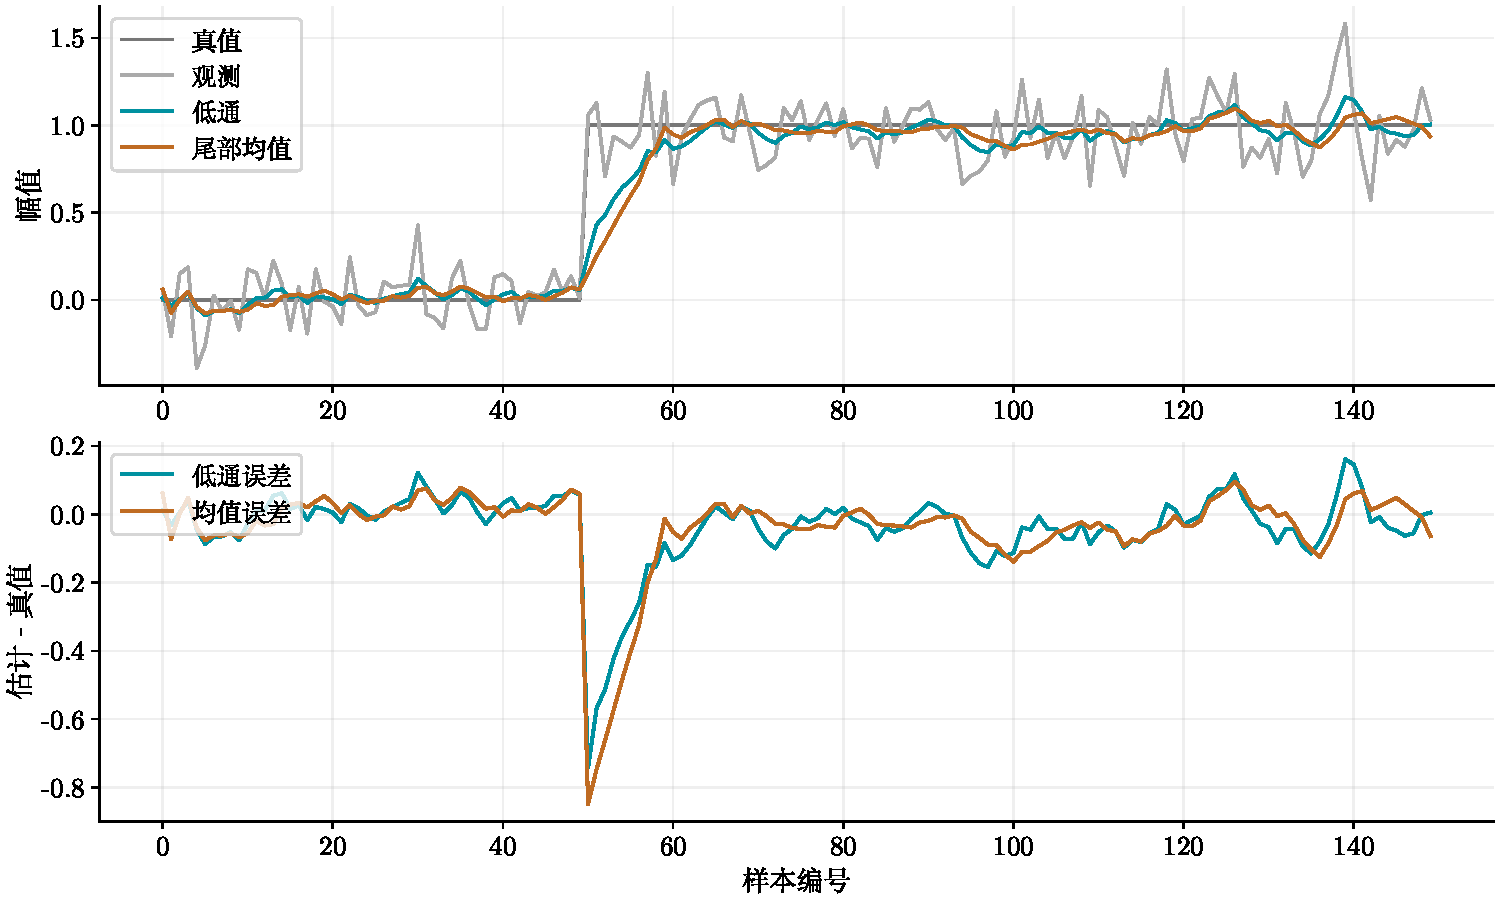
\includegraphics[width=.94\textwidth]{images/filter_smooth_revised.pdf}
\caption{实际保存的模拟序列：阶跃后的偏差与整段误差一起看，不能只挑静止部分}
\label{fig:v2-filter-smooth}
\end{figure}
\begin{exercise}\label{ex:v2-filter-lowpass}
对连续输入1、初值0，手算 $a=0.2$、0.5、1 的前三步。运行各变体，记录达到无噪声阶跃90\%的更新次数，解释与整段 RMSE 的区别。
\end{exercise}
\begin{conclusion}
先确定你想保留的信号，再决定平滑方式。尾部窗口和递归低通都可能跟随滞后；高通保留快速变化也可能保留噪声。至少同时看真值误差与变化后的响应，输出方差变小不是单独的合格证。
\end{conclusion}

\subsubsection{从两份估计推到融合权重}
卡尔曼滤波（Kalman Filter，KF）看上去有一堆矩阵，不过它的更新可以先从两份估计讲起。假设 $X=p+N_1$、$Y=p+N_2$ 都无偏，噪声均值为0，方差分别为 $\sigma^2,\tau^2$，先假定彼此独立。我们用
\[
\hat p=wX+(1-w)Y
\]
融合，均值仍为 $p$；方差为 $w^2\sigma^2+(1-w)^2\tau^2$。对 $w$ 求导并令其为0，得到
\[
w=\frac{\tau^2}{\sigma^2+\tau^2},\qquad
\operatorname{Var}(\hat p)=\frac{\sigma^2\tau^2}{\sigma^2+\tau^2}.
\]
这就是逆方差加权：越不确定的那份估计，权重越小。高斯分布并不是“任何噪声都长这样”，这里方差推导只需要上述二阶统计与独立条件。

如果两份结果来自同一张图，它们可能共享误差。记交叉协方差为 $c=\operatorname{Cov}(N_1,N_2)$，则
\[
\operatorname{Var}(\hat p)
=w^2\sigma^2+(1-w)^2\tau^2+2w(1-w)c,\qquad
w=\frac{\tau^2-c}{\sigma^2+\tau^2-2c}.
\]
最后一个分母为正时才按此求唯一最优权重。完全相同、等方差的噪声使分母为0，重复平均不会增加信息。某些相关条件下最优权重还可能超出0--1，不要拿独立情形的直觉硬套。

\paragraph*{从信号功率再看一次*}
若共同信号为 $s(t)$，两路零均值噪声与它及彼此不相关，$s_1=s+N_1,s_2=s+N_2$，那么
\[
E[s_1s_2]=E[s^2],\qquad
E[(ws_1+(1-w)s_2)^2]
=E[s^2]+w^2\sigma^2+(1-w)^2\tau^2.
\]
共同信号保留，噪声功率按权重变化，仍得到前面的结论。独立性不会让交叉项凭空多出两份噪声方差；如果噪声相关，就重新加入 $2w(1-w)c$。

\begin{example}[真的把相关性算进去]
\path{fusion.py} 使用方差与相关系数 $\rho$ 得到 $c=\rho\sqrt{\sigma^2\tau^2}$，并完整计算融合方差：
\lstinputlisting[numbers=left,language=Python,basicstyle=\footnotesize\ttfamily]{examples/filter/state-estimation-demo/fusion.py}
\begin{tbash}
python3 fusion.py
python3 fusion.py --v2 1 --rho 0
python3 fusion.py --v2 1 --rho 1
\end{tbash}
默认两估计2/4、方差1/3，输出权重0.75、均值2.5、方差0.75。两方差都为1且独立，方差变为0.5；完全正相关时仍为1。最后一条主要检查统计公式的退化情况：等方差、完全相同的无偏噪声在实际同一次采样中应给出相同读数，不能拿代码固定的2/4当这种联合分布的有效样本。
\end{example}
\begin{exercise}\label{ex:v2-filter-fusion}
将第二个方差改为1，算均值与独立融合方差；再令 $\rho=1$，解释为何不能把同一帧派生的两份信息当成两次独立测量。
\end{exercise}

\subsubsection{状态、协方差和预测：把“小滑块”写进程序}
真实追踪不一定有两个传感器，不过我们还有上一时刻的估计。假设一个小滑块沿直线运动，短时间内速度近似不变，用状态 $\boldsymbol x=[p,v]^T$ 记录位置和速度，单位为 m 与 m/s：
\[
F=\begin{bmatrix}1&\Delta t\\0&1\end{bmatrix},\qquad
H=\begin{bmatrix}1&0\end{bmatrix}.
\]
$F$ 把速度换成这段时间的位置变化，$H$ 只取位置作为观测。只测位置不等于速度永远不可估，连续位置及运动模型提供了时间约束；但约束是否足够还要检查系统可观性。
\begin{figure}[htbp]
\centering
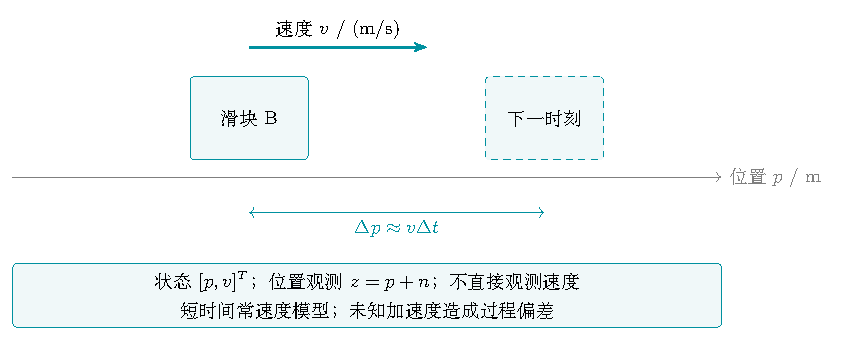
\includegraphics[width=.9\textwidth]{images/filter_motion_revised.pdf}
\caption{沿一维方向运动的小滑块：位置观测配合时间模型估计速度}
\label{fig:F_filter-1}
\end{figure}
更一般的状态与观测可写成
\[
\boldsymbol x_k=F_k\boldsymbol x_{k-1}+B_k\boldsymbol u_k+\boldsymbol w_k,\qquad
\boldsymbol z_k=H_k\boldsymbol x_k+\boldsymbol n_k.
\]
控制输入可省略，本项目不把未知真实加速度当作已知控制。过程噪声 $\boldsymbol w_k$ 协方差为 $Q_k$，观测噪声 $\boldsymbol n_k$ 协方差为 $R_k$；我们先采用零均值、加性并与先前误差相应独立的模型。时间戳要决定实际 $\Delta t$，乱序、丢帧和不规则采样不能一直装作每次都是0.1秒。

\paragraph*{协方差不是一排“可信度分数”}
二维协方差写成
\[
P=\begin{bmatrix}\sigma_p^2&c_{pv}\\c_{pv}&\sigma_v^2\end{bmatrix}.
\]
对角线是各分量方差，非对角线是协方差；$P_{pp}$ 的单位是 m$^2$，$P_{vv}$ 是 (m/s)$^2$，$P_{pv}$ 是 m$^2$/s，不能都写成同一个无单位小数。矩阵须对称半正定，负方差不能解释成“特别有信心”。对独立随机向量，和的协方差相加；相关时还要加交叉协方差及其转置。线性变换满足
\[
E[A\boldsymbol x]=AE[\boldsymbol x],\qquad
\operatorname{Cov}(A\boldsymbol x)=A P A^T.
\]
因此预测不只推进均值，还传播误差：
\begin{equation}
\boldsymbol x_k^-=F_k\boldsymbol x_{k-1}^++B_k\boldsymbol u_k,\qquad
P_k^-=F_kP_{k-1}^+F_k^T+Q_k.
\label{eq:Px}
\end{equation}
上标减号表示看到新观测之前，称先验（prior）；加号表示更新之后，称后验（posterior），不是给状态加减一个常量。

相关系数 $\rho=c_{pv}/(\sigma_p\sigma_v)$ 在方差非零时位于 $[-1,1]$。它不是椭圆短长轴之比，也不是协方差非对角线的乘积。零相关、等方差的联合高斯等密度线是圆；方差不同就可能是轴对齐椭圆。一般分布中零相关也不保证独立。
\begin{figure}[htbp]
\centering
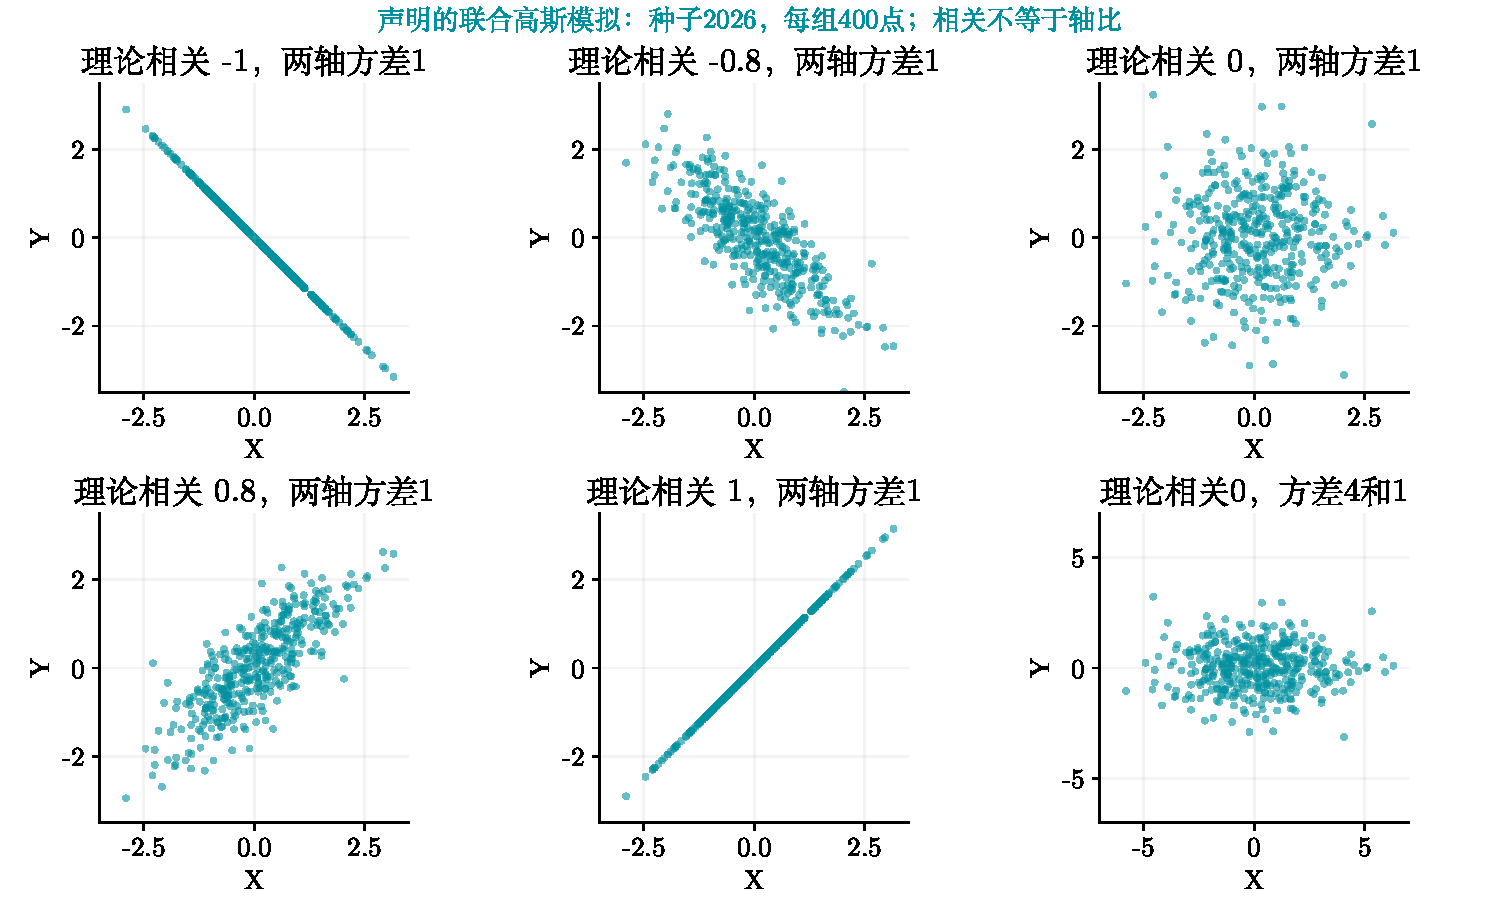
\includegraphics[width=.94\textwidth]{images/filter_covariance_revised.pdf}
\caption{明确生成条件的相关性示意；右下零相关但两轴方差不同，不是圆}
\label{fig:related}
\end{figure}

\begin{example}[给 Q 一个能核对单位的模型]
本项目假定每段内有一个未知、零均值的加速度扰动，方差为 $q_a$，令
\[
G=\begin{bmatrix}\Delta t^2/2\\\Delta t\end{bmatrix},\qquad
Q=q_aGG^T.
\]
这是离散“每段一个随机加速度”的模型，不是连续白噪声谱密度公式；两者的 $q$ 单位和时间幂次不同。$\Delta t=0.1$ s、$q_a=0.5$ (m/s$^2$)$^2$ 时，
\[
Q=\begin{bmatrix}0.0000125&0.00025\\0.00025&0.005\end{bmatrix}.
\]
下面项目的 run 正是按此生成 Q，不直接给位置和速度各塞一个相同方差。R=0.04 m$^2$ 对应位置标准差0.2 m。
\end{example}
\begin{exercise}\label{ex:v2-filter-covariance}
写出上述 F、H、Q 的尺寸和各项单位。把 $\Delta t$ 改为0.05 s，计算新的 Q，解释为何不能只改 F 而沿用原 Q。
\end{exercise}

\subsubsection{Kalman 更新：先比较观测，再修正状态}
看到新位置后，我们先问“它和模型预期差多少”，而不是去求 $H^{-1}$。H 往往是长方形，根本没有普通逆矩阵。创新量（innovation）和它的协方差为
\[
\boldsymbol r_k=\boldsymbol z_k-H_k\boldsymbol x_k^-,
\qquad S_k=H_kP_k^-H_k^T+R_k.
\]
然后将创新映回状态空间：
\begin{align}
K_k&=P_k^-H_k^TS_k^{-1},\\
\boldsymbol x_k^+&=\boldsymbol x_k^-+K_k\boldsymbol r_k.
\label{eq:final}
\end{align}
$P_k^-$ 为 $n\times n$，H 为 $m\times n$，S 为 $m\times m$，所以 K 为 $n\times m$。这一维位置观测可以同时修正位置和速度，靠的是预测后两者的协方差联系。在标量 H=1 的情形，R 变小通常增大对观测的权重；矩阵 K 的各项不能都当作0--1的置信度。

\paragraph*{为什么是这个增益*}
令误差为“估计减真值”，更新后有 $\boldsymbol e^+=(I-KH)\boldsymbol e^-+K\boldsymbol n$。先验误差与观测噪声不相关时，后验协方差为
\[
P^+=(I-KH)P^-(I-KH)^T+KRK^T.
\]
这称 Joseph 形式。对 $\operatorname{tr}(P^+)$ 关于 K 求导，得到
\[
\frac{\partial\operatorname{tr}(P^+)}{\partial K}
=-2P^-H^T+2K(HP^-H^T+R).
\]
令其为0就回到前面的增益。如果 S 可逆，在精确运算中还能化为 $P^+=(I-KH)P^-$；实际程序保留 Joseph 形式，有助于减轻浮点误差破坏对称性和非负性的风险。矩阵求解不必显式构造逆，更不能用逐元素除法假装矩阵逆。

\begin{example}[把预测和更新写完整]
\path{linear.py} 检查协方差，再预测；更新时用 \texttt{solve} 解线性方程，最后算完整 Joseph 形式。末尾对称化只消除微小浮点不对称，遇到明显负特征值仍报错，不靠“加个数”掩盖模型错误：
\lstinputlisting[numbers=left,language=Python,basicstyle=\footnotesize\ttfamily]{examples/filter/state-estimation-demo/linear.py}
\path{scalar.py} 把它接成原来的手算例：随机游走、初值0、P=1、Q=0.1、R=0.9、第一次观测2。
\lstinputlisting[numbers=left,language=Python,basicstyle=\footnotesize\ttfamily]{examples/filter/state-estimation-demo/scalar.py}
\begin{minipage}{\linewidth}
\begin{tbash}
python3 scalar.py
python3 scalar.py --r 9
\end{tbash}
\end{minipage}
先验方差1.1，默认 K=0.55、更新状态1.1、方差0.495；改R=9时 K约0.108911，状态约0.217822，方差约0.980198。这里只改假定观测方差，其余完全一样，才能解释权重为什么改变。
\end{example}
\begin{exercise}\label{ex:v2-filter-scalar}
手算 R=9 的 K、状态与方差，再与程序核对。说明 Q、R、P 分别属于哪里，为什么不能交换预测与更新的顺序。
\end{exercise}
\begin{figure}[htbp]
\centering
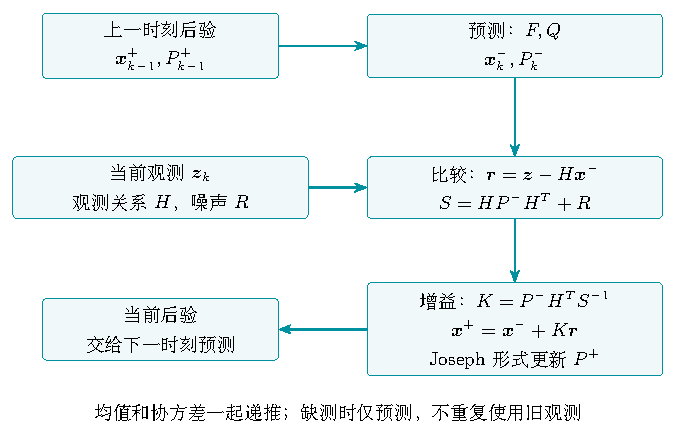
\includegraphics[width=.94\textwidth]{images/filter_flow_revised.pdf}
\caption{上一时刻后验先预测，再与当前观测比较；同时推进均值和协方差}
\label{fig:kalman}
\end{figure}
\begin{conclusion}
KF 更新的是状态估计及其误差协方差，并没有拿到每一步真实误差。先用 F/Q 预测，再用 H/R 与新观测更新；P 描述当前估计不确定性，S 描述创新不确定性。在线性、零均值且满足相应不相关条件时，KF 给出最优线性估计；联合高斯条件下对应最小均方误差估计。模型、单位或偏置错了，漂亮的矩阵也救不了。
\end{conclusion}

\subsubsection{把一步手算接成一段轨迹}
前面的一步很容易算对，不过追踪还要面对持续运动、加速和缺测。先看 \path{data.py}：起点1 m、速度0.3 m/s，中间三分之一施加0.7 m/s$^2$加速度，其他时段为0；观测加标准差0.2 m的噪声。真实加速度用于生成真值，不传给滤波器。位置与斜距使用同一份噪声，方便后面比较，不拿它们当独立传感器融合。
\begin{example}[同一输入同时跑两种估计]
\lstinputlisting[numbers=left,language=Python,basicstyle=\footnotesize\ttfamily]{examples/filter/state-estimation-demo/data.py}
\path{run.py} 先规定模式、时间和方差，再逐步执行预测/更新。linear 直接观测位置，range 则观测斜距；UKF 的实现稍后完整展开。
\lstinputlisting[numbers=left,language=Python,basicstyle=\footnotesize\ttfamily,firstline=1,lastline=29]{examples/filter/state-estimation-demo/run.py}
接下来给 UKF 相同初值，准备输出数组，再进入逐帧循环。当一帧缺测，只预测，P 仍继续传播；有观测时计算创新与归一化创新平方 $\mathrm{NIS}=r^2/S$。本项目只观测一个标量，向量观测则使用 $\boldsymbol r^TS^{-1}\boldsymbol r$，不能逐项随意除。
\lstinputlisting[numbers=left,language=Python,basicstyle=\footnotesize\ttfamily,firstnumber=30,firstline=30]{examples/filter/state-estimation-demo/run.py}
\begin{tbash}
python3 run.py --mode linear --output out/linear
python3 run.py --mode linear --q 0 --output out/q0
python3 run.py --mode linear --drop-every 5 --output out/drops
\end{tbash}
dt 单位秒；q 为每段加速度方差，r 为观测方差；bias 给观测加固定偏置，seed 决定随机数据，drop-every=5 每五帧跳过一次更新，alpha 属于后面的无迹变换。默认150步，本次 KF 位置 RMSE约0.1385 m；丢帧变体跳过30次更新。Q=0表示我们假定匀速模型没有过程不确定性，但模拟目标仍会加速，看看输出在这段怎样落后。

程序保存真值、观测、估计、创新和 NIS，并记录全过程的协方差最小特征值。这里的特征值是当前状态坐标下的数值检查，换单位会改变数值，不能把它当跨单位的物理评分。NIS 均值约1可以作标量模型下的检查线索，但不能凭一次小样本的平均值就确认模型正确；还要看创新的均值、相关性、变化时段和参数假设。
\end{example}

\begin{example}[用保存的数组画图]
\path{plot.py} 只读前面输出，不在画图时重算滤波。它默认使用教材已有中文字体，也可通过 --font 指定字体文件：
\lstinputlisting[numbers=left,language=Python,basicstyle=\footnotesize\ttfamily]{examples/filter/state-estimation-demo/plot.py}
\begin{tbash}
python3 plot.py --input out/smooth/series.npz --output out/smooth.pdf
python3 plot.py --input out/linear/series.npz --output out/linear.pdf
\end{tbash}
滤波曲线、真值误差和创新分开看。若想改变参数，先运行 run 保存新数组，再绘图；不要只改图上的标签。
\end{example}
\begin{figure}[htbp]
\centering
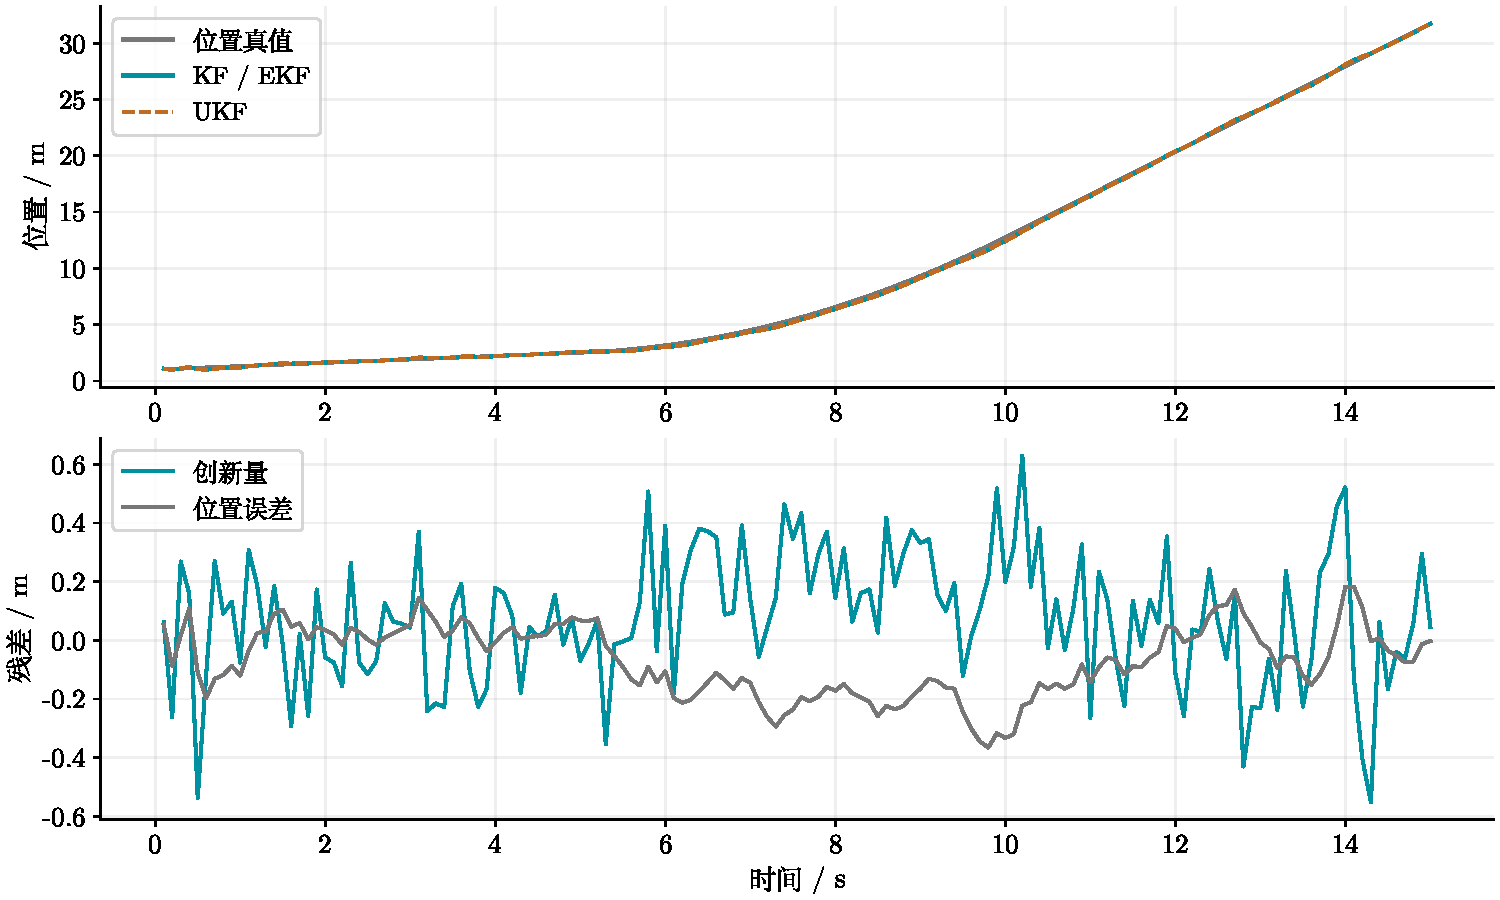
\includegraphics[width=.94\textwidth]{images/filter_track_revised.pdf}
\caption{实际模拟轨迹的 KF/UKF 输出与创新；线性模式下两者结果几乎重合}
\label{fig:v2-filter-track}
\end{figure}
\begin{exercise}\label{ex:v2-filter-track}
分别运行默认、Q=0、R=0.4 和缺测变体，用独立目录保存。记录 RMSE、NIS、协方差最小特征值与加速段表现；再加入0.5 m偏置，说明为什么平滑不能保证无偏。项目准备、状态模型与序列运行在这道综合练习中一起核对。
\end{exercise}

\subsubsection{非线性观测：EKF 线性化的是哪里}
如果观测直接是位置，H 只是取一个分量；若测的是距离，事情就不同了。设传感器与运动轨道垂直间距固定为2 m，水平位置为 p，斜距观测为
\[
h(\boldsymbol x)=\sqrt{p^2+2^2}.
\]
这不是把位置乘一个常量能得到的关系。距离也不能单独区分 $p$ 与 $-p$；本实验给定正侧轨道及初始状态，不宣称解决了全局符号歧义。

扩展卡尔曼滤波（Extended Kalman Filter，EKF）对均值使用实际非线性函数，对误差传播使用局部雅可比。一般加性模型为 $\boldsymbol x_k=f(\boldsymbol x_{k-1})+\boldsymbol w_k$、$\boldsymbol z_k=h(\boldsymbol x_k)+\boldsymbol n_k$；观测函数的输入是状态，不是拿观测 z 自己喂自己。预测雅可比 $F_k$ 在上一时刻后验处求，观测雅可比 $H_k$ 在当前先验处求。本项目过程仍线性，观测雅可比为
\[
H_k=\begin{bmatrix}p^-/\sqrt{(p^-)^2+4}&0\end{bmatrix}.
\]
创新用 $z-h(\boldsymbol x^-)$，不能改成 $z-H_k\boldsymbol x^-$；雅可比不是原函数。随后用这个 H 传播创新协方差与增益，状态按原函数的创新更新。

\begin{example}[用同一份 run 检查 EKF]
run 中 range 分支正是先计算 h，再求 H，把 h 的结果作为 update 的 expected。执行：
\begin{tbash}
python3 run.py --mode range --output out/range
python3 plot.py --input out/range/series.npz --output out/range.pdf
\end{tbash}
默认条件下本次 EKF 位置 RMSE约0.1535 m，UKF约0.1568 m。这个实验中 UKF 没有更准，名字更高级不等于当前模型一定更好。接近 p=0 时距离的一阶位置导数很小，局部更新较弱；初值错误、模型歧义或很大不确定性都会影响求解。
\end{example}
\begin{exercise}\label{ex:v2-filter-ekf}
在 p=1 m处计算 h 与 H 的非零项，手算 $h(1.001)-h(0.999)$ 的差分导数并比较。指出 EKF 创新中为什么必须保留 h；描述 p=0 时的局部约束问题。
\end{exercise}

\subsubsection{无迹变换：传播几个点，再重建统计量}
局部线性化会漏掉曲率的影响。我们保留原来的例子：$X\sim U(-1,1)$，$Y=X^2+X$。由 $E[X]=0$、$E[X^2]=1/3$、$E[X^4]=1/5$ 得
\[
E[Y]=\frac13,\qquad
\operatorname{Var}(Y)=\frac15+\frac13-\frac19=\frac{19}{45}.
\]
在0处的一阶近似却是 $Y\approx X$，给出均值0、方差1/3。问题并不在乘法写错，而在“先取均值再过函数”通常不等于“过函数后取均值”。

无迹变换（Unscented Transform，UT）换一种思路：用少量确定选择的 sigma 点匹配均值与协方差，将点送进真实函数，再按权重重建统计量。它不是 Monte Carlo 的随机采样，也不保证有限个点能准确描述任意非线性或任意分布的高阶矩。

\paragraph*{取点与权重要一起看}
对于 n维、正定协方差P，NumPy 的 Cholesky 分解给出下三角 L，使 $P=LL^T$。取点使用 L 的列；如果你换成上三角因子，就要相应换方向。常见缩放 UT 定义
\[
\lambda=\alpha^2(n+\kappa)-n,\qquad c=n+\lambda>0.
\]
用 $L_cL_c^T=cP$ 得到
\begin{equation}
\chi_0=\boldsymbol x,\qquad
\chi_i=\boldsymbol x+(L_c)_{:i},\qquad
\chi_{n+i}=\boldsymbol x-(L_c)_{:i},\quad i=1,\ldots,n.
\label{eq:sigma}
\end{equation}
两侧是相反方向，缩放包含平方根，不能把 $(n-\lambda)L$ 当作另一半点。均值与协方差权重分别为
\[
W_0^{(m)}=\frac{\lambda}{c},\quad
W_0^{(c)}=\frac{\lambda}{c}+1-\alpha^2+\beta,\quad
W_i^{(m)}=W_i^{(c)}=\frac1{2c}.
\]
非中心点的分子是1，不是 $\lambda$。$\alpha$ 控制展开尺度，$\kappa$ 配合维度缩放，$\beta$ 纳入分布先验；高斯输入常用 $\beta=2$，不代表所有分布都具有高斯四阶矩。参数可能产生负权重，取很小 alpha 还可能放大浮点消减误差；本项目默认 alpha=1、kappa=0、beta=2，不把它说成通用最优值。Cholesky 要求正定，半正定奇异矩阵需要专门处理，不能一概声称所有协方差都可直接分解。

\begin{example}[重建后再说取点正确]
\path{sigma.py} 将 L 的各列变为行排列的点，\texttt{moments} 重建均值与协方差：
\lstinputlisting[numbers=left,language=Python,basicstyle=\footnotesize\ttfamily]{examples/filter/state-estimation-demo/sigma.py}
\path{moments_demo.py} 首先重建非对角协方差，再传播仿射函数，最后回到均匀分布的非线性例子：
\lstinputlisting[numbers=left,language=Python,basicstyle=\footnotesize\ttfamily]{examples/filter/state-estimation-demo/moments_demo.py}
\begin{tbash}
python3 moments_demo.py
\end{tbash}
重建原均值[1,2]与协方差后，仿射结果应等于 $A\boldsymbol x+b$ 和 $APA^T$。非线性例中，这组 UT 得到均值1/3，却得到方差5/9，仍不同于均匀分布真值19/45；输出同时给出20万次声明的随机抽样对照。这恰好说明匹配前两阶统计量并不足以指定所有高阶矩。不能只展示这次均值对了，就宣布 UKF 对任何函数都准确。
\end{example}
\begin{figure}[htbp]
\centering
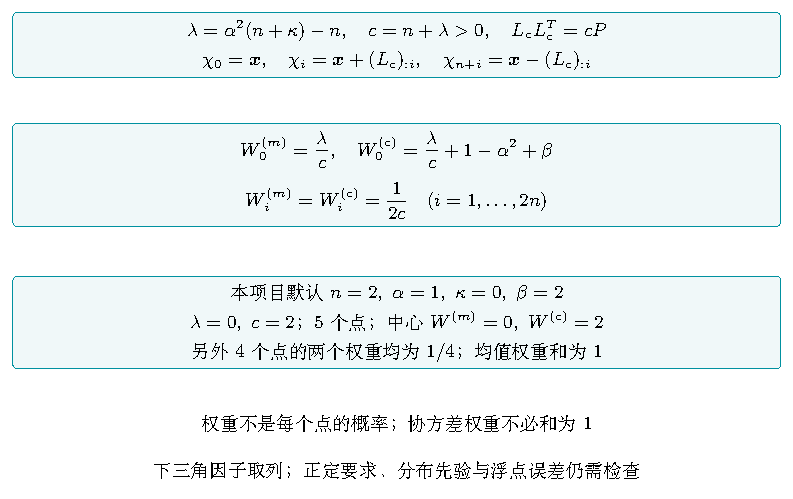
\includegraphics[width=.94\textwidth]{images/filter_weights_revised.pdf}
\caption{缩放 UT 的点、权重与默认二维数值；中心均值权重0也仍需保留中心协方差权重}
\label{fig:weight}
\end{figure}
\begin{exercise}\label{ex:v2-filter-ut}
用现有 sigma 点传播 $y=2x+1$，计算均值与方差，与线性公式比较。再核对均匀输入 $X^2+X$ 的精确方差与本次 UT 方差，解释两种结论为什么可以同时成立。
\end{exercise}

\subsubsection{UKF：把无迹变换接回预测与更新}
无迹卡尔曼滤波（Unscented Kalman Filter，UKF）把前面的取点、传播、重建接成递归估计。本项目采用独立加性过程/观测噪声：先将点过状态函数得到先验均值与协方差，加 Q，再基于完整先验重新取点、传播观测。重新取点是为了让观测统计也包含过程噪声；本章没有展开非加性噪声的增广状态版本。

记先验观测均值为 $\bar z$，状态和观测的离差为 $\delta x_i,\delta z_i$，则
\[
P_{xz}=\sum_i W_i^{(c)}\delta x_i\delta z_i^T,\qquad
S=P_{zz}=\sum_i W_i^{(c)}\delta z_i\delta z_i^T+R,
\]
\begin{equation}
K=P_{xz}S^{-1},\qquad
\boldsymbol x^+=\boldsymbol x^-+K(\boldsymbol z-\bar z),\qquad
P^+=P^--KSK^T.
\label{eq:ukf-K}
\end{equation}
矩阵时仍是求解，不是分子分母逐元素相除。本项目仅一个标量观测，所以 S 是标量；代码的 \texttt{cross/S} 在这个限定下才是正确运算。

\begin{example}[完整 UKF 和两种模式的对照]
\lstinputlisting[numbers=left,language=Python,basicstyle=\footnotesize\ttfamily]{examples/filter/state-estimation-demo/ukf.py}
\begin{tbash}
python3 run.py --mode linear --output out/linear
python3 run.py --mode range --alpha 0.3 --output out/range-a03
\end{tbash}
默认线性模式下 KF 与 UKF 的全过程状态最大差约 $9.8\times10^{-15}$，是浮点量级；这支持取点、Q传播与更新在此模型下相符。range 模式就不要求两者相同，也不承诺 UKF 总能胜出。缺测时两个程序只返回预测，收到下一帧再更新，不能将旧观测反复当作新的独立信息。
\end{example}
\begin{exercise}\label{ex:v2-filter-ukf}
n=2、alpha=1、kappa=0、beta=2时计算 lambda、点数、中心及其他权重。运行 linear/range 及 alpha=0.3 变体，记录状态差、RMSE和协方差；解释为何需要先加 Q 再取观测点。
\end{exercise}
\begin{conclusion}
KF 直接传播线性统计量，EKF 传播均值与局部雅可比，UKF 传播选定点。三者都需要正确模型、单位和噪声假设。把重建、仿射传播、创新、误差和协方差连起来检查，既不因为曲线抖就一味调 R，也不因为名字里带“最优”就省略验证。
\end{conclusion}
\begin{note}
线性 KF 与 EKF 的经典介绍可查 Welch 与 Bishop 的
\href{https://www.cs.utexas.edu/~pstone/Courses/393Rfall15/readings/Welch+Bishop-TR-95.pdf}{An Introduction to the Kalman Filter（大学课程镜像）}；
缩放无迹变换和 UKF 见 Wan 与 van der Merwe 的
\href{https://groups.seas.harvard.edu/courses/cs281/papers/unscented.pdf}{The Unscented Kalman Filter for Nonlinear Estimation}。
先按本章小例子把尺寸和统计量算通，再阅读一般系统与增广噪声版本。
\end{note}


\section{本章小结}
\begin{conclusion}
我们从抖动的读数出发，先区分过程变化、观测误差与系统性偏置，再看平滑带来的延迟。接下来把位置和速度组成状态，用 F/Q 推进估计，用 H/R 与新观测比较，均值和协方差一起递推。KF、EKF、UKF 的区别主要在怎样传播统计量，而不是谁的名字更长谁就更好。

你应能核对状态单位、矩阵尺寸、创新和协方差，跑通手算与同一序列的比较。遇到非线性，先写清 h 和雅可比求值位置，再检查 sigma 点是否重建原来的统计量。一般推导可以继续查文献，但曲线是否跟得上、偏置是否残留、缺测时有没有重复使用旧信息，这些不能留到“以后再说”。
\end{conclusion}

\begin{problemset}
\item\label{prob:v2-filter-noise} 未建模加速度、传感器随机误差和固定零偏分别怎样处理？解释为什么三者不能一股脑用“大一点的R”解决。
\item\label{prob:v2-filter-response} 一阶低通初值0、输入恒为2、系数0.25，前两步输出是多少？若采样间隔加倍而系数不变，以秒计的相同响应会怎样变化？高通互补输出各是多少？
\item\label{prob:v2-filter-gain} 先验方差2、观测方差3、H=1，先验值4、观测值9，计算增益、更新状态与后验方差。若H变为1行2列，为什么不能用普通逆将位置观测直接变成完整状态？
\item\label{prob:v2-filter-related} 两个独立无偏估计的方差都为4，平均后的方差是多少？若是同一个估计复制两次，方差是多少？说明交叉协方差怎样进入计算。
\item\label{prob:v2-filter-units} 状态位置用m、速度用m/s，观测直接填mm，会造成什么？写出P的三种不同单位，并说明R=0.04与观测标准差的关系。
\item\label{prob:v2-filter-q} 对本章每段随机加速度模型，采样间隔减半时，Q的位置项、交叉项、速度项分别缩小到原来的多少？说明为何这不能直接用于另一种连续白噪声模型。
\item\label{prob:v2-filter-nonlinear} EKF 与 UKF 分别怎样处理非线性？对斜距观测说明EKF创新为什么用 h 而不是 Hx；再解释UT匹配前两阶统计量为何不保证任意分布的非线性方差准确。
\item\label{prob:v2-filter-missing} 第五帧没有新观测时，估计器应怎样递推？为什么不能拿第四帧重复更新？同时说明协方差变小并不能单独证明跟踪误差变小。
\item\label{prob:v2-filter-scalar} 运行一步更新，把R从0.9改为9，提交两次K、x、P和手算核对；随后尝试R=0，记录程序怎样拒绝无效输入。
\item\label{prob:v2-filter-experiment} 运行linear默认、Q=0、固定0.5 m偏置与range变体，分别保存实际数组和指标。指出加速段与偏置段的误差，解释哪一组更适合当前任务，不能只凭曲线更平下结论。
\end{problemset}

\section{本章验收}
请检查者看你实际保存的输入和输出，并现场改一个参数重跑；图上的文字要对应这次运行，不能拿旧图代替新结果。
\begin{enumerate}
\item 在本章项目目录运行平滑实验，展示原始、低通、尾部均值及误差曲线，改alpha后核对无噪声阶跃90\%响应次数，并演示高通与低通相加还原输入。
\item 解释位置/速度状态、F/H和Q/R的尺寸、单位与生成条件，现场核对scalar的一步预测/更新，再运行linear序列；提交真实RMSE、创新/NIS、协方差最小特征值及Q=0或缺测对照。
\item 用非对角P运行sigma重建与仿射传播，核对解析均值和协方差；展示均匀输入非线性例的近似偏差，指出权重、Cholesky因子取列和正定条件。
\item 在同一range序列上比较EKF/UKF，说明雅可比的求值位置、h的创新和UKF加Q后重新取点的原因。展示一次alpha变体与固定偏置对照；按模型、误差和残差解释结果，不要求某个算法必然获胜。
\end{enumerate}


% ============================================================
\chapter{几何视觉与 Bundle Adjustment}

\begin{introduction}
  \item 学习目标：计算投影与坐标变换，运行DLT/PnP与候选核对；验证旋转、指数更新和像素雅可比；完成位姿优化、联合BA及最近邻ICP实验。
  \item 建议学时：约 1--1.5 周。
  \item 本卷边界：聚焦几何模型与数值核对；相机采集标定见本卷相机章，装甲板坐标定义和赛场工程见卷三。
\end{introduction}

\section{投影、位姿与几何优化}


\subsubsection{投影与相机模型}

\begin{figure}[H]
    \centering
    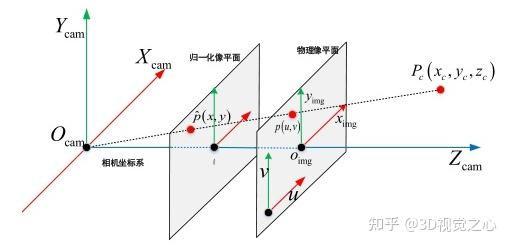
\includegraphics[width=0.8\linewidth]{相机模型.jpg}
    \caption{相机成像过程：CMOS应该位于透镜后，图中作了修改以便于理解}
    \label{fig:camera}
\end{figure}

相机成像的过程可以简单的看做是一个投影的过程，如图\ref{fig:camera}所示。
相机成像的核心是一个CMOS传感器，其上分布有许多区域，对应着图像中的一个像素点。
当光线通过相机镜头时，会在CMOS传感器上形成一个像素点的亮斑，这个亮斑的中心位置就是图像中的一个像素点。

CMOS传感器是一个平面，被称为\textbf{成像平面}，距离镜头光心的距离被称为\textbf{焦距}。
应用相似三角形的原理，可以进行投影变换。

\begin{equation}
    \begin{aligned}
        \frac{X}{Z} &= \frac{U}{f_x} \\
        \frac{Y}{Z} &= \frac{V}{f_y}
    \end{aligned}
\end{equation}

我们一般将图像坐标系的原点设置在图像的角，需要给方程添加一个偏移量，写成矩阵形式就是：

\begin{equation}
    \begin{bmatrix}
        U \\
        V
    \end{bmatrix} =
    \begin{bmatrix}
        f_x & 0 \\
        0 & f_y
    \end{bmatrix}
    \begin{bmatrix}
        X/Z \\
        Y/Z
    \end{bmatrix} +
    \begin{bmatrix}
        c_x \\
        c_y
    \end{bmatrix}
\end{equation}

做一下维数统一，引入\textbf{齐次坐标}：

\begin{equation}
    \begin{bmatrix}
        U \\
        V \\
        1
    \end{bmatrix} = \frac{1}{Z}
    \begin{bmatrix}
        f_x & 0 & c_x \\
        0 & f_y & c_y \\
        0 & 0 & 1
    \end{bmatrix}
    \begin{bmatrix}
        X \\
        Y \\
        Z
    \end{bmatrix}
\end{equation}

这就是最基本的相机模型。

\begin{example}
无畸变针孔模型中，fx=fy=800、cx=320、cy=240，相机坐标 (0.2,0.1,2) m 投影为 (400,280) pixel。
\begin{tpython}
fx,fy,cx,cy=800,800,320,240
X,Y,Z=0.2,0.1,2.0
u,v=fx*X/Z+cx,fy*Y/Z+cy
assert (u,v)==(400,280)
print(u,v)
\end{tpython}
\end{example}

\begin{exercise}
把距离 Z 加倍，计算新的像素坐标。说明像素坐标为何不是简单除以 2。
\end{exercise}

\subsubsection{相机内参与标定}

实际中镜头并不是理想的，会产生畸变，所以仅直到焦距这些数据并不足以完整地描述相机成像过程中的坐标变换关系。
引入畸变矩阵$\mathbf{D}$，使其与原来的投影矩阵$\mathbf{C}$相乘，得到内参矩阵$\mathbf{K}$：

\begin{equation}
    \begin{bmatrix}
        U \\
        V \\
        1
    \end{bmatrix} = \frac{1}{Z} \mathbf{K}
    \begin{bmatrix}
        X \\
        Y \\
        Z
    \end{bmatrix}
\end{equation}

我们不对畸变矩阵进行过多的讨论，对于畸变的产生和消除也不做过多的探讨，因为其与当前主题无关，
主要关注于内参矩阵$\mathbf{K}$的标定。

\begin{figure}[H]
    \centering
    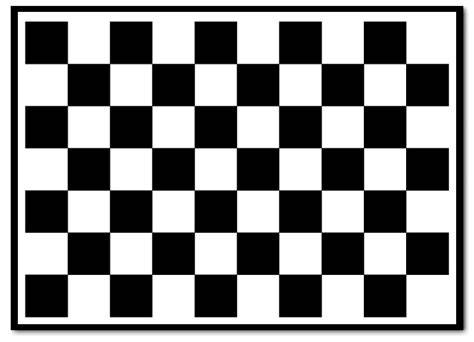
\includegraphics[width=0.8\linewidth]{标定板.jpeg}
    \caption{相机标定：\textbf{一般采用张正友标定法}}
    \label{fig:calibration}
\end{figure}

使用ROS的calibration包可以很方便地进行相机标定，标定的过程主要是通过拍摄一系列不同位置和姿态的标定板（如图\ref{fig:calibration}所示），来计算出相机的内参矩阵$\mathbf{K}$。
标定的结果包括焦距、主点位置和畸变参数等，这些参数对于后续的图像处理和空间位置解算非常重要。

\begin{example}
原图 640×480，fx=800、cx=320。仅进行各方向等比例 0.5 缩放且不裁剪时，fx 变为 400、cx 变为 160；标准归一化畸变系数保持不变。若裁剪左侧 20 pixel，主点还要相应平移。
\end{example}

\begin{exercise}
原图 fy=820、cy=240，缩小到一半后再从顶部裁去 10 pixel，求新的 fy 与 cy。
\end{exercise}

\subsubsection{坐标系变换与相机外参}
除了相机成像的过程，要想实现自瞄系统，就需要对目标进行空间位置解算，这就需要引入坐标系变换的概念。

\paragraph*{三维空间刚体运动}
三维空间中，通过设置一组基向量$[\mathbf{e_1},\mathbf{e_2},\mathbf{e_3}]$，就可以通过线性变换表示这个空间中任意一个点的位置。
\begin{equation}
    \mathbf{a} = [\mathbf{e_1},\mathbf{e_2},\mathbf{e_3}] [a_1, a_2, a_3]^T
\end{equation}

$[a_1, a_2, a_3]^T$是点$\mathbf{a}$在此基下的坐标。

现在来分析坐标系之间的关系，$\mathbf{P}$分解在两个坐标系下。

\begin{equation}
    \mathbf{P} = [\mathbf{e_1},\mathbf{e_2},\mathbf{e_3}] 
    \begin{bmatrix}
        a_1 \\
        a_2 \\
        a_3
    \end{bmatrix}
    = [\mathbf{e_1'},\mathbf{e_2'},\mathbf{e_3'}] 
    \begin{bmatrix}
        a_1' \\
        a_2' \\
        a_3'
    \end{bmatrix}
\end{equation}

在两边乘上$[\mathbf{e_1},\mathbf{e_2},\mathbf{e_3}]^{-1}$，
也就是 $[\mathbf{e_1},\mathbf{e_2},\mathbf{e_3}]^T$
得到：

\begin{equation}
    \begin{bmatrix}
        a_1 \\
        a_2 \\
        a_3
    \end{bmatrix}
    =
    \begin{bmatrix}
        \mathbf{e_1}^T \mathbf{e_1'} & \mathbf{e_1}^T \mathbf{e_2'} & \mathbf{e_1}^T \mathbf{e_3'} \\
        \mathbf{e_2}^T \mathbf{e_1'} & \mathbf{e_2}^T \mathbf{e_2'} & \mathbf{e_2}^T \mathbf{e_3'} \\
        \mathbf{e_3}^T \mathbf{e_1'} & \mathbf{e_3}^T \mathbf{e_2'} & \mathbf{e_3}^T \mathbf{e_3'}
    \end{bmatrix}
    \begin{bmatrix}
        a_1' \\
        a_2' \\
        a_3'
    \end{bmatrix}
    \overset{\text{def}}{=}
    \mathbf{R}\mathbf{a'}
\end{equation}

这里的$\mathbf{R}$就是坐标系之间的\textbf{旋转矩阵}，描述了两个坐标系之间的旋转关系。
旋转矩阵还有一些特别的性质，他是一个行列式为1的正交矩阵，可以对n维旋转矩阵进行下面的定义：
\begin{equation}
    SO(n) = \{\mathbf{R} \in \mathbb{R}^{n \times n} | \mathbf{R}^T\mathbf{R} = \mathbf{I}, \det(\mathbf{R}) = 1\}
\end{equation}
$SO(n)$是\textbf{特殊正交群}，描述了n维空间中的旋转变换。$SO(3)$表示三维空间中的旋转变换。
$R^T$ 刻画了一个相反的旋转关系，因为$R^{-1} = R^T$。

欧式变换中，除了旋转之外还有平移。$a$经过一次旋转$R$和平移$t$之后得到$a'$，可以表示为：
\begin{equation}
    \mathbf{a'} = \mathbf{R}\mathbf{a} + \mathbf{t}
\end{equation}

这里还有一个问题，这个变换不是线性的，我们可以通过引入\textbf{齐次坐标}来将其转化为线性变换。
\begin{equation}
    \begin{bmatrix}
        a' \\
        1
    \end{bmatrix} =
    \begin{bmatrix}
        \mathbf{R} & \mathbf{t} \\
        \mathbf{0}^T & 1
    \end{bmatrix}
    \begin{bmatrix}
        a \\
        1
    \end{bmatrix}
    \overset{\text{def}}{=}
    \mathbf{T}[\mathbf{a},1]^T
\end{equation}

$\mathbf{T}$被称为\textbf{变换矩阵}，描述了两个坐标系之间的旋转和平移关系。

\begin{equation}
    SE(n) = \{\mathbf{T}|\mathbf{T} = 
    \begin{bmatrix}
        \mathbf{R} & \mathbf{t} \\
        \mathbf{0}^T & 1
    \end{bmatrix}, \mathbf{R} \in SO(n), \mathbf{t} \in \mathbb{R}^n\}
\end{equation}

$SE(n)$被称为\textbf{特殊欧式群}，描述了n维空间中的旋转和平移变换。$SE(3)$表示三维空间中的旋转和平移变换。
与$SO(3)$类似，$SE(3)$也有一个相反的变换关系，可以通过求逆来得到：
\begin{equation}
    \mathbf{T}^{-1} =
    \begin{bmatrix}
        \mathbf{R}^T & -\mathbf{R}^T\mathbf{t} \\
        \mathbf{0}^T & 1
    \end{bmatrix}
\end{equation}

也可以简写成 $\mathbf{a}' = \mathbf{Ta}$ ，这里隐含一个齐次坐标与非齐次坐标的转换，并不是简单的矩阵乘法，否则是不成立的。
这种表述后文也会出现，不再赘述。

SO(n)和SE(n)是李群，具有连续性和平滑性，可以通过指数映射和对数映射在李代数和李群之间进行转换。
这些性质在~\ref{sec:李代数}中会有简要的介绍。

\paragraph*{自瞄系统的常见坐标系}
在自瞄系统中，常见的坐标系主要有以下几种：

\textbf{图像坐标系：} 图像坐标系是以图像中心为原点，x轴和y轴分别指向图像的右侧和下方的坐标系，z轴指向图像平面的法线方向.

\textbf{相机坐标系：} 相机坐标系是以相机光心为原点，z轴指向相机前方，x轴和y轴分别指向相机的右侧和下方的坐标系，原点在相机成像平面中心.

\textbf{云台系：} 云台系是以云台旋转中心为原点，x轴指向云台前方，y轴和z轴分别指向云台的右侧和上方的坐标系，圆点在云台旋转中心.

\textbf{世界坐标系：} 自瞄系统的世界系指的是，上电初始位置的云台坐标系，但是不与云台绑定，始终保持不变.

\paragraph*{相机外参}

指的是描述相机坐标系与世界坐标系之间关系的变换矩阵$\mathbf{T}$，它包含了旋转和平移两个部分。
一般来说，相机的位态都可以称为相机外参，一般是相对于世界系的，但是在不同的应用场景和需求下，也不绝对。

\begin{example}
列向量约定下，R 为单位阵，t=(1,0,0)。物体点 (0,2,3) 变到相机系为 (1,2,3)；逆变换应恢复原点坐标。需要 NumPy。
\begin{tpython}
import numpy as np
R=np.eye(3); t=np.array([1.,0.,0.])
p=np.array([0.,2.,3.])
q=R@p+t
recovered=R.T@(q-t)
assert np.allclose(q,[1,2,3]) and np.allclose(recovered,p)
print(q,recovered)
\end{tpython}
\end{example}

\begin{exercise}
绕 z 轴旋转 90°，平移不变，手算并修改 R 验证结果。
\end{exercise}

\subsubsection{PnP问题与求解}

PnP问题是指在已知空间中n个点的坐标以及它们在图像中的投影位置的情况下，求解相机的位姿（位置和姿态）的问题。

\paragraph*{直接线性变换DLT}

直接考虑这样一个问题：已知一组3D点的位置，以及他们在某个相机中的投影位置，求解该相机的位姿。

考虑某个空间点$\mathbf{P}=(X, Y, Z)^T$，在图像中特征点$\mathbf{p}=(u_1, v_1,1)^T$。
我们定义一个增广矩阵$[\mathbf{R} | \mathbf{t}]$，有$\mathbf{p} = [\mathbf{R} | \mathbf{t}] \mathbf{P}$，
展开来写就是：

\begin{equation}
    d\begin{bmatrix}
        u_1 \\
        v_1 \\
        1
    \end{bmatrix}
    =
    \begin{bmatrix}
        t_{1} & t_{2} & t_{3} & t_4 \\
        t_{5} & t_{6} & t_{7} & t_8 \\
        t_{9} & t_{10} & t_{11} & t_12
    \end{bmatrix}
    \begin{bmatrix}
        X \\
        Y \\
        Z \\
        1
    \end{bmatrix}
\end{equation}

使用最后一行把$d$消掉，得到两个约束：

\begin{equation}
    \begin{aligned}
        u_1 = \frac{t_1X+t_2Y+t_3Z+t_4}{t_9X+t_{10}Y+t_{11}Z+t_{12}} \\
        v_1 = \frac{t_5X+t_6Y+t_7Z+t_8}{t_9X+t_{10}Y+t_{11}Z+t_{12}} 
    \end{aligned}
\end{equation}

做一些简化表示：

\begin{equation}
    \begin{aligned}
        \mathbf{t_1} = (t_1,t_2,t_3,t_4)^T \\
        \mathbf{t_2} = (t_5,t_6,t_7,t_8)^T \\
        \mathbf{t_3} = (t_9,t_{10},t_{11},t_{12})^T
    \end{aligned}
\end{equation}

于是有：

\begin{equation}
    \begin{aligned}
        \mathbf{t_1}^T\mathbf{P} - \mathbf{t_3}^T\mathbf{P}u_1 = 0 \\
        \mathbf{t_2}^T\mathbf{P} - \mathbf{t_3}^T\mathbf{P}v_1 = 0  
    \end{aligned}
\end{equation}

$\mathbf{t}$是待求的变量，可以看到，每个特征点可以提供两个方程，至少需要6个特征点就可以求解出$\mathbf{t}$。

\begin{equation}
    \begin{bmatrix}
        \mathbf{P_1}^T & \mathbf{0}^T & -u_1\mathbf{P_1}^T \\
        \mathbf{0}^T & \mathbf{P_1}^T & -v_1\mathbf{P_1}^T \\
        \vdots & \vdots & \vdots \\
        \mathbf{P_n}^T & \mathbf{0}^T & -u_n\mathbf{P_n}^T \\
        \mathbf{0}^T & \mathbf{P_n}^T & -v_n\mathbf{P_n}^T
    \end{bmatrix}
    \begin{bmatrix}
        \mathbf{t_1} \\
        \mathbf{t_2} \\
        \mathbf{t_3}
    \end{bmatrix} = \mathbf{0}
\end{equation}

这种方法被称为\textbf{直接线性变换DLT}。当匹配点的数量大于6时，可以通过$SVD$等方法对超定方程求最小二乘解。

在DLT求解中，我们忽略了$\mathbf{T}$的各元素关系。旋转矩阵$R \in SO(3)$，DLT求解得到的$\mathbf{T}$不一定满足这个约束，所以需要对求解结果进行后续处理，来满足旋转矩阵的约束。
若内参已知，先恢复旋转部分并消除尺度，再做旋转投影。满秩时可用极分解，例如：

\begin{equation}
    \mathbf{R} \gets (\mathbf{R}\mathbf{R}^T)^{-\frac{1}{2}}\mathbf{R}
\end{equation}

内外参分离与旋转投影的区别见后文(参考~\ref{sec:DLT的QR求解} 和~\ref{sec:DLT的极分解求解})。

\paragraph*{P3P}

P3P是另一种求解PnP问题的方法，它仅使用三对匹配点，对数据要求较少。

\begin{figure}[H]
    \centering
    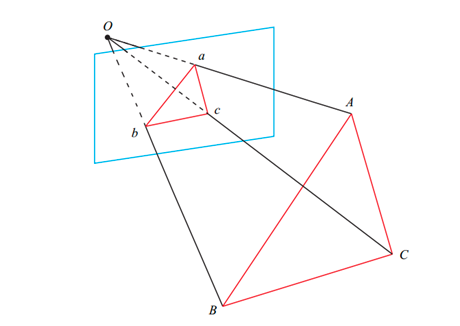
\includegraphics[width=0.99\linewidth]{p3p.png}
    \caption{P3P求解示意图}
    \label{fig:P3P}
\end{figure}

以图~\ref{fig:P3P}为例，已知空间中三个点$A, B, C$的位置，以及它们在图像中的投影位置$a, b, c$，求解相机的位姿。

显然存在一些几何上的相似关系：
\begin{equation}
    \begin{aligned}
        \bigtriangleup Oab \sim \bigtriangleup OAB \\
        \bigtriangleup Obc \sim \bigtriangleup OBC \\
        \bigtriangleup Oca \sim \bigtriangleup OCA
    \end{aligned}
\end{equation}

列写余弦定理的方程：
\begin{equation}
    \begin{aligned}
        OA^2 +OB^2 -2OA\cdot OB \cdot \cos<a,b> = AB^2 \\
        OB^2 +OC^2 -2OB\cdot OC \cdot \cos<b,c> = BC^2 \\
        OC^2 +OA^2 -2OC\cdot OA \cdot \cos<c,a> = CA^2
    \end{aligned}
\end{equation}

令$x = \frac{OA}{OC}, y = \frac{OB}{OC}$，全体除以$OC^2$，得到：
\begin{equation}
    \begin{aligned}
        x^2 + y^2 - 2xy\cos<a,b> = \frac{AB^2}{OC^2} \\
        y^2 + 1 - 2y\cos<b,c> = \frac{BC^2}{OC^2} \\
        1 + x^2 - 2x\cos<c,a> = \frac{CA^2}{OC^2}
    \end{aligned}
\end{equation}

记$v=\frac{AB^2}{OC^2}$，$uv=\frac{BC^2}{OC^2}$，$wv=\frac{AC^2}{OC^2}$，得到：
\begin{equation}
    \begin{aligned}
        x^2 + y^2 - 2xy\cos<a,b> - v = 0 \\
        y^2 + 1 - 2y\cos<b,c> - uv = 0 \\
        x^2 + 1 - 2x\cos<c,a> - wv = 0
    \end{aligned}
\end{equation}

将第一个式子的$v$带入第二、三个式子，得到：
\begin{equation}
    \begin{aligned}
        (1-u)y^2 - ux^2 - y\cos<b,c> + 2uxy\cos<a,b> + 1 = 0 \\
        (1-w)x^2 - wy^2 - x\cos<a,c> + 2wxy\cos<a,b> + 1 = 0
    \end{aligned}
\end{equation}

重新审视这个方程组，由于我们知道2D点的图像位置，所以可以计算出<a,b>、<b,c>、<c,a>的值，
空间点的位置也已知，所以可以计算出$u$和$w$的值。
所以事实上是一个关于$x,y$的二元二次方程。

这个方程的解析解求解过程非常复杂，需要用到吴消元法，在此不再讨论。
计算得到$x,y,v$的值就可以推算出$OA,OB,OC$的值，也就是计算出了相机系下的点坐标，我们称之为3D-3D点对，转换为了ICP问题，
从而可以求解出相机的位姿。ICP求解相较于PnP是比较简单的，具体方法可以参考~\ref{sec:ICP求解}。

P3P也存在一些问题：
\begin{itemize}
    \item P3P只利用3个点的信息。当给定的配对点多余3组时，难以利用多余的信息
    \item 如果3D点或2D点存在噪声，或存在误匹配，则算法失效
\end{itemize}

\begin{example}
用已知位姿合成八个非共面的点，再调用 solvePnP 恢复。Python 环境需 numpy 与 opencv-python。无噪声时重投影均方根误差应小于 0.001 pixel。
\begin{tpython}
import cv2
import numpy as np
obj=np.array([[x,y,z] for x in [-.1,.1] for y in [-.1,.1]
              for z in [0.,.2]],dtype=np.float64)
K=np.array([[800.,0,320],[0,800,240],[0,0,1]])
dist=np.zeros(5)
r=np.array([.1,.2,0.]); t=np.array([0.,0.,2.])
image,_=cv2.projectPoints(obj,r,t,K,dist)
ok,r_hat,t_hat=cv2.solvePnP(obj,image,K,dist,flags=cv2.SOLVEPNP_ITERATIVE)
if not ok: raise RuntimeError("PnP 求解失败")
reprojected,_=cv2.projectPoints(obj,r_hat,t_hat,K,dist)
rms=np.sqrt(np.mean(np.sum((reprojected-image)**2,axis=2)))
assert rms < 1e-3
print(t_hat.ravel(),rms)
\end{tpython}
\end{example}

\begin{exercise}
打乱两个二维点的对应顺序，比较误差。说明只看求解函数返回成功为何不够。
\end{exercise}

\begin{note}
solvePnP 输出把物体系点变到相机系的旋转和平移。点数要求取决于解法；共面、共线与错误对应都可能造成歧义或退化。
\end{note}

\subsubsection{最小化重投影误差BA}

除了使用线性方法，还可以把PnP问题构建成一个关于重投影误差的非线性最小二乘问题。
可以用它对PnP或ICP的结果进行优化，得到更准确的位姿估计。
这一类把相机和三维点放在一起优化的问题，统称为\textbf{Bundle Adjustment}，简称BA。

\paragraph*{问题引入}

考虑\(n\)个三维空间点\(P\)和它们的投影\(p\)，我们希望基于此计算相机位姿。假设某点\(\mathbf{P}\_i=[X\_i,Y\_i,Z\_i]^T\)，其投影\(\mathbf{p}\_i=[u\_i,v\_i]^T\)，相机位姿的李群表示为\(\mathbf{T}\)。它们的空间位置关系可以表示为：
\begin{equation}
    s_i\begin{bmatrix}
        u_i \\
        v_i \\
        1
    \end{bmatrix}
    =
    \mathbf{K}\mathbf{T}
    \begin{bmatrix}
        X_i \\
        Y_i \\
        Z_i \\
        1
    \end{bmatrix}
\end{equation}

也就是：
\begin{equation}
    s_i\mathbf{p}_i = \mathbf{K}\mathbf{T}\mathbf{P}_i
\end{equation}

由于噪声存在，上面的这个等式不再成立，可以让它的两边的差距最小化，得到一个非线性最小二乘问题，求解最优的\(\mathbf{T}\)：
\begin{equation}
    \mathbf{T}^* = \arg\min_{\mathbf{T}} \frac{1}{2}\sum_{i=1}^n \|s_i\mathbf{p}_i - \mathbf{K}\mathbf{T}\mathbf{P}_i\|^2_2
\end{equation}

更一般地，设\(z\_{ij}\)为在位姿\(\boldsymbol{\xi}\_i\)处观察路标\(\mathbf{p}\_j\)产生的像素坐标，观测方程抽象为：
\begin{equation}
    z_{ij} = h(\boldsymbol{\xi}_i, \mathbf{p}_j)
\end{equation}
其中\(\boldsymbol{\xi}\_i\)为相机位姿\(\mathbf{T}\_i\)对应的李代数。观测误差定义为：
\begin{equation}
    \mathbf{e}_{ij} = z_{ij} - h(\boldsymbol{\xi}_i, \mathbf{p}_j)
\end{equation}

将相邻时刻的观测全部考虑进来，整体的BA代价函数为：
\begin{equation}\label{eq:ba_cost}
    F(\mathbf{x}) = \frac{1}{2}\sum_{i=1}^m\sum_{j=1}^n \|\mathbf{e}_{ij}\|^2
    = \frac{1}{2}\sum_{i=1}^m\sum_{j=1}^n \|z_{ij} - h(\boldsymbol{\xi}_i, \mathbf{p}_j)\|^2
\end{equation}
其中\(\mathbf{x} = [\boldsymbol{\xi}\_1, \dots, \boldsymbol{\xi}\_m, \mathbf{p}\_1, \dots, \mathbf{p}\_n]^T\)为所有待优化的变量，包括所有相机位姿和三维路标点。对这个最小二乘进行求解，相当于对位姿和路标同时进行调整，这就是BA。

\paragraph*{求解方法}

观测模型\(h(\boldsymbol{\xi}, \mathbf{p})\)是非线性函数，因此需要使用非线性优化手段来求解。根据高斯—牛顿法（G-N）或列文伯格—马夸尔特法（L-M），我们从某个初始值开始，不断地寻找下降方向\(\Delta\mathbf{x}\)来逼近目标函数的最优解。

对代价函数在\(\mathbf{x}\)处进行一阶泰勒展开：
\begin{equation}
    F(\mathbf{x}+\Delta\mathbf{x}) \approx \frac{1}{2}\sum_{i=1}^m\sum_{j=1}^n \|\mathbf{e}_{ij} + \mathbf{F}_{ij}\Delta\boldsymbol{\xi}_i + \mathbf{E}_{ij}\Delta\mathbf{p}_j\|^2
\end{equation}
其中\(\mathbf{F}\_{ij}\)为代价函数对相机位姿的偏导数，\(\mathbf{E}\_{ij}\)为代价函数对路标点位置的偏导数。令：
\begin{equation}
    \mathbf{J} = [\mathbf{F} \quad \mathbf{E}], \quad \Delta\mathbf{x} = [\Delta\boldsymbol{\xi}^T, \Delta\mathbf{p}^T]^T
\end{equation}

则整体代价函数可以紧凑地写为：
\begin{equation}
    F(\mathbf{x}+\Delta\mathbf{x}) \approx \frac{1}{2}\|\mathbf{e} + \mathbf{J}\Delta\mathbf{x}\|^2
\end{equation}

对\(\Delta\mathbf{x}\)求导并令其为零，得到增量方程（正规方程）：
\begin{equation}\label{eq:normal_equation}
    \mathbf{H}\Delta\mathbf{x} = \mathbf{g}
\end{equation}
其中\(\mathbf{H} = \mathbf{J}^T\mathbf{J}\)为信息矩阵，\(\mathbf{g} = -\mathbf{J}^T\mathbf{e}\)。

\textbf{雅可比矩阵的形式：} 基于李代数的扰动模型（左扰动），重投影误差关于相机位姿扰动量\(\delta\boldsymbol{\xi}\)的雅可比矩阵为：
\begin{equation}
    \begin{aligned}
        \frac{\partial \mathbf{e}}{\partial \delta\boldsymbol{\xi}} 
        = \lim_{\delta \mathbf{\xi} \to 0}\frac{\mathbf{e}(\delta \mathbf{\xi} \oplus \mathbf{\xi})-e(\mathbf{\xi})}{\delta\boldsymbol{\xi}}
        = \frac{\partial \mathbf{e}}{\partial \mathbf{p}}\frac{\partial \mathbf{p}}{\partial \delta\boldsymbol{\xi}}\\
    \end{aligned}
\end{equation}

其中$\oplus$表示李代数上的左乘扰动。第一项是误差关于投影点的导数。已知投影关系：
\begin{equation}
    u=f_x\frac{X'}{Z'}+c_x, v=f_y\frac{Y'}{Z'}+c_y
\end{equation}
其中\([X',Y',Z']^T\)为空间点在相机坐标系下的坐标。那么易得：
\begin{equation}
    \begin{aligned}
        \frac{\partial \mathbf{e}}{\partial \mathbf{p}} &=-
        \begin{bmatrix}
        \frac{\partial e_u}{\partial X'} & \frac{\partial e_u}{\partial Y'} & \frac{\partial e_u}{\partial Z'} \\
        \frac{\partial e_v}{\partial X'} & \frac{\partial e_v}{\partial Y'} & \frac{\partial e_v}{\partial Z'} 
        \end{bmatrix} \\
        &=-
        \begin{bmatrix}
        \frac{f_x}{Z'} & 0 & -\frac{f_x X'}{Z'^2} \\
        0 & \frac{f_y}{Z'} & -\frac{f_y Y'}{Z'^2}
        \end{bmatrix}
    \end{aligned}
\end{equation}

第二项是投影点关于位姿扰动的导数。
\begin{equation}
    \begin{aligned}
        \frac{\partial \mathbf{TP}}{\partial \delta\boldsymbol{\xi}} = (\mathbf{TP})^\odot = \begin{bmatrix}
        \mathbf{I} & -\mathbf{P}^{'\wedge} \\
        0^T & 0^T
        \end{bmatrix}
    \end{aligned}
\end{equation}
由于$\mathbf{TP}=\begin{bmatrix} \mathbf{P}' \\ 1 \end{bmatrix}$，我们只选取前三维度，因此：
\begin{equation}
    \frac{\partial \mathbf{p}}{\partial \delta\boldsymbol{\xi}} = \begin{bmatrix}
        \mathbf{I} & -\mathbf{P}^{'\wedge}
    \end{bmatrix}
\end{equation}

相乘得到：
\begin{equation}
    -\begin{bmatrix}
        \frac{f_x}{Z'} & 0 & -\frac{f_x X'}{Z'^2} & -\frac{f_x X'Y'}{Z'^2} & f_x+\frac{f_x X'^2}{Z'^2} & -\frac{f_x Y'}{Z'} \\[6pt]
        0 & \frac{f_y}{Z'} & -\frac{f_y Y'}{Z'^2} & -f_y-\frac{f_y Y'^2}{Z'^2} & \frac{f_y X'Y'}{Z'^2} & \frac{f_y X'}{Z'}
    \end{bmatrix}
\end{equation}
这就是重投影误差关于相机位姿扰动的雅可比矩阵。

又有$\frac{\partial \mathbf{p}}{\partial \mathbf{P}}=\mathbf{R}$



重投影误差关于空间点\(\mathbf{P}\)的雅可比矩阵为：
\begin{equation}
    \frac{\partial \mathbf{e}}{\partial \mathbf{P}} = -
    \begin{bmatrix}
        \frac{f_x}{Z'} & 0 & -\frac{f_x X'}{Z'^2} \\[6pt]
        0 & \frac{f_y}{Z'} & -\frac{f_y Y'}{Z'^2}
    \end{bmatrix}
    \mathbf{R}
\end{equation}
其中\(\mathbf{R}\)为旋转矩阵。

拿到偏导数之后，后面的事情就很简单了，使用GN或者LM等优化方法就可以进行迭代求解了。为了减少迭代次数，可以使用PnP或ICP的结果作为BA的初始值。

\textbf{稀疏性与舒尔消元：} \(\mathbf{H}\)矩阵具有典型的稀疏结构——相机位姿之间、路标点之间的关联分别形成分块对角结构，而位姿与路标点之间则通过观测形成关联。将\(\mathbf{H}\)按相机位姿部分\(\mathbf{H}\_{cc}\)和空间点部分\(\mathbf{H}\_{pp}\)进行分块：
\begin{equation}
    \begin{bmatrix}
        \mathbf{H}_{cc} & \mathbf{H}_{cp} \\
        \mathbf{H}_{pc} & \mathbf{H}_{pp}
    \end{bmatrix}
    \begin{bmatrix}
        \Delta\mathbf{x}_c \\
        \Delta\mathbf{x}_p
    \end{bmatrix}
    =
    \begin{bmatrix}
        \mathbf{g}_c \\
        \mathbf{g}_p
    \end{bmatrix}
\end{equation}

利用\(\mathbf{H}\_{pp}\)为对角块矩阵的性质，可通过舒尔消元（Schur消元，也称边缘化，Marginalization）将空间点部分消去：
\begin{equation}
    (\mathbf{H}_{cc} - \mathbf{H}_{cp}\mathbf{H}_{pp}^{-1}\mathbf{H}_{pc})\Delta\mathbf{x}_c
    = \mathbf{g}_c - \mathbf{H}_{cp}\mathbf{H}_{pp}^{-1}\mathbf{g}_p
\end{equation}

先求解上式得到相机位姿的增量\(\Delta\mathbf{x}\_c\)，再回代求得空间点的增量：
\begin{equation}
    \Delta\mathbf{x}_p = \mathbf{H}_{pp}^{-1}(\mathbf{g}_p - \mathbf{H}_{pc}\Delta\mathbf{x}_c)
\end{equation}

这种方法大大降低了增量方程的维度，使得BA即使在包含大量路标点的情况下也能高效求解。

\begin{example}
用标量平移展示最小二乘更新：预测值为 x+t，观测值比 x 大 2。残差平方和在 t=2 时为 0。该例只演示优化目标，不代表完整 BA。
\begin{tpython}
x=[0.,1.,2.]; observed=[2.,3.,4.]
t=sum(y-a for a,y in zip(x,observed))/len(x)
cost=sum((a+t-y)**2 for a,y in zip(x,observed))
assert t==2 and cost==0
print(t,cost)
\end{tpython}
\end{example}

\begin{exercise}
把最后一个观测改为 10，计算最优 t。解释异常点为何会拉动普通最小二乘解。
\end{exercise}

\subsubsection{BA与图优化}

BA问题可以很自然地表示成图优化（Graph Optimization）的形式。在图优化框架中，将待优化的变量（相机位姿和三维路标点）作为图的\textbf{顶点（Vertex）}，将观测方程作为连接对应位姿顶点和路标顶点的\textbf{边（Edge）}。边的约束由重投影误差定义，优化的目标即调整所有顶点的位置，使得所有边的误差之和最小。

图优化将SLAM问题直观地表达为一个稀疏图的结构，便于利用图的性质进行高效的优化求解。随着时间推移，地图规模会不断增长，计算效率面临挑战。BA中大量特征点的存在导致计算量随路标数量快速增长。在更大规模的场景中，通常采用两种策略来控制BA的规模：

（1）\textbf{滑动窗口法：} 固定优化\(N\)个关键帧，这\(N\)个关键帧同时观测到\(M\)个路标点，从而建立一个规模适中的BA问题。窗口外（时间上较远）的帧和路标被边际化（Marginalization），转化为先验信息加入优化当中。

（2）\textbf{位姿图（Pose Graph）：} 当特征点的数量远大于相机位姿数量时，路标点在经过若干次优化后通常已基本收敛。此时不再继续优化路标点的位置，而仅把它们视为对位姿节点的约束，从而得到一个只包含相机位姿顶点的图优化问题。

在位姿图中，节点\(\boldsymbol{\xi}\_i\)和\(\boldsymbol{\xi}\_j\)之间的一条边，对应于两者之间的相对运动估计\(\Delta\boldsymbol{\xi}\_{ij}\)。该相对运动的观测方程可抽象为：
\begin{equation}
    \Delta\boldsymbol{\xi}_{ij} = \boldsymbol{\xi}_i^{-1} \circ \boldsymbol{\xi}_j
\end{equation}
或以李代数表示为：
\begin{equation}
    \Delta\boldsymbol{\xi}_{ij} = \ln\bigl(\exp((-\boldsymbol{\xi}_i)^\wedge)\,\exp(\boldsymbol{\xi}_j^\wedge)\bigr)^\vee
\end{equation}

则位姿图的误差项（即边的代价）可定义为：
\begin{equation}
    \mathbf{e}_{ij} = \ln\bigl(\mathbf{T}_{ij}^{-1}\,\mathbf{T}_i^{-1}\,\mathbf{T}_j\bigr)^\vee
\end{equation}
其中\(\mathbf{T}\_{ij}\)为从\(i\)到\(j\)的观测相对位姿。整体的位姿图优化目标函数为：
\begin{equation}\label{eq:pose_graph_cost}
    \min_{\boldsymbol{\xi}} \frac{1}{2}\sum_{i,j\in\mathcal{E}} \mathbf{e}_{ij}^T\,\boldsymbol{\Sigma}_{ij}^{-1}\,\mathbf{e}_{ij}
\end{equation}

其中\(\mathcal{E}\)为所有边的集合，\(\boldsymbol{\Sigma}\_{ij}\)为信息矩阵。位姿图将BA中大量的路标点“收缩”为位姿间的约束，
其优化问题的规模远远小于完整的BA，因此在大规模建图中具有重要的实用价值。所有节点的位姿仍旧可以利用非线性优化方法（如G-N法或L-M法）进行迭代求解，
其最终形式与增量方程(公式~\ref{eq:normal_equation})一致，只是自变量的维度被大幅压缩。

工程上常采用g2o、Ceres等图优化库来实现BA和位姿图优化，这些库提供了高效的稀疏矩阵求解器和灵活的接口，支持各种类型的误差项和约束。

\begin{example}
两个相机观测同一个三维点，可画成两个位姿顶点、一个路标顶点和两条观测边。若同时平移所有相机与路标，图像不变；优化时必须固定参考坐标系，避免规范自由度导致不唯一。
\end{example}

\begin{exercise}
三个相机分别观测两个路标，且观测全部存在。统计顶点与边数，标出可固定的参考顶点。
\end{exercise}

\subsubsection{基于 QR 与 RQ 分解的内外参分离}\label{sec:DLT的QR求解}

在针孔相机模型中，投影矩阵 $\mathbf{P}$ 可分解为内参矩阵 $\mathbf{K}$（上三角，对角元为正）与位姿矩阵的乘积：
\[
\mathbf{P} = \mathbf{K}[\mathbf{R}\mid\mathbf{t}].
\]
DLT直接估计出 $\mathbf{P}$ 后，取其左边 $3\times3$ 的子矩阵
\[
\mathbf{M} = \mathbf{P}_{:,1:3} = \mathbf{K}\mathbf{R}.
\]
这里需要的是 RQ 分解（上三角矩阵在左、正交矩阵在右），而不是直接把普通 QR 的结果交换名字：
\[
\mathbf{M}=\mathbf{K}\mathbf{R}.
\]
普通 QR 给出 $\mathbf{M}=\mathbf{Q}\mathbf{R}_{\mathrm{up}}$，通常不能令 $\mathbf{Q}=\mathbf{R}$、$\mathbf{R}_{\mathrm{up}}=\mathbf{K}$。
RQ 可借助行列反序后的 QR 实现，也可使用 OpenCV 的 \texttt{RQDecomp3x3}。
处理投影矩阵的整体尺度与符号后，应核对内参对角元为正、$R^TR=I$、$\det R=1$；最后将 $K_{33}$ 归一化为 1。
如果已知 $K$，则先计算 $K^{-1}M$，消除尺度，再按下一节的 SVD 方法投影到旋转矩阵集合。
\begin{note}
QR、RQ 与旋转投影解决的问题不同。交换两个矩阵的乘法顺序，通常会改变结果。
\end{note}

\begin{example}
使用 OpenCV 的 RQ 分解验证 M=KR，而不是直接交换 QR 的结果。已知内参对角元为正，示例不含投影矩阵的整体尺度歧义。
\begin{tpython}
import cv2
import numpy as np
K=np.array([[800.,10,320],[0,820,240],[0,0,1]])
R,_=cv2.Rodrigues(np.array([.1,.2,.3]))
M=K@R
result=cv2.RQDecomp3x3(M)
K_hat,R_hat=result[1],result[2]
assert np.allclose(K_hat@R_hat,M)
assert np.allclose(K_hat,K) and np.allclose(R_hat,R)
print(np.linalg.det(R_hat))
\end{tpython}
\end{example}

\begin{exercise}
用 numpy.linalg.qr(M) 替换分解，检查重建顺序，并验证其正交因子是否等于原 R。
\end{exercise}

\subsubsection{基于极分解的旋转矩阵投影}\label{sec:DLT的极分解求解}

任意方阵 $\tilde{\mathbf{R}}$（由DLT得到的含噪声旋转部分）可寻找一个在Frobenius范数意义下最接近的正交矩阵 $\mathbf{Q}$，即求解正交Procrustes问题：
\[
\mathbf{Q}^* = \arg\min_{\mathbf{Q}^T\mathbf{Q}=\mathbf{I}} \|\mathbf{Q} - \tilde{\mathbf{R}}\|_F^2.
\]
展开目标函数得
\[
\|\mathbf{Q} - \tilde{\mathbf{R}}\|_F^2 = 3 + \|\tilde{\mathbf{R}}\|_F^2 - 2\,\mathrm{tr}(\mathbf{Q}^T\tilde{\mathbf{R}}),
\]
因此最小化等价于最大化 $\mathrm{tr}(\mathbf{Q}^T\tilde{\mathbf{R}})$。对 $\tilde{\mathbf{R}}$ 作奇异值分解：
\[
\tilde{\mathbf{R}} = \mathbf{U}\boldsymbol{\Sigma}\mathbf{V}^T,\quad \boldsymbol{\Sigma}=\mathrm{diag}(\sigma_1,\sigma_2,\sigma_3),\ \sigma_i\ge0.
\]
于是
\[
\mathrm{tr}(\mathbf{Q}^T\tilde{\mathbf{R}}) = \mathrm{tr}(\mathbf{V}^T\mathbf{Q}^T\mathbf{U}\,\boldsymbol{\Sigma}) = \mathrm{tr}(\mathbf{Z}\,\boldsymbol{\Sigma}),
\]
这里 $\mathbf{Z}=\mathbf{V}^T\mathbf{Q}^T\mathbf{U}$ 为正交矩阵。为使迹 $\sum_{i}z_{ii}\sigma_i$ 最大，须有 $z_{ii}=1$ 且其余元素为 $0$，故 $\mathbf{Z}=\mathbf{I}$，得最优解
\[
\mathbf{Q} = \mathbf{U}\mathbf{V}^T.
\]
此即 $\tilde{\mathbf{R}}$ 的极分解中的正交因子。利用等式
\[
(\tilde{\mathbf{R}}^T\tilde{\mathbf{R}})^{-\frac12} = \mathbf{V}\boldsymbol{\Sigma}^{-1}\mathbf{V}^T,
\]
可以写出等价形式
\[
\mathbf{Q} = \tilde{\mathbf{R}}\,(\tilde{\mathbf{R}}^T\tilde{\mathbf{R}})^{-\frac12},
\]
该式要求矩阵满秩；退化或接近奇异时，优先使用 SVD。为保证最终结果为旋转矩阵 ($\det=+1$)，需附加修正：
\[
\mathbf{R}^* = \mathbf{U}\,\mathrm{diag}\big(1,\,1,\,\det(\mathbf{U}\mathbf{V}^T)\big)\,\mathbf{V}^T.
\]
当 $\det(\mathbf{U}\mathbf{V}^T)=1$ 时，$\mathbf{R}^* = \mathbf{U}\mathbf{V}^T$；当其为 $-1$ 时，将最后一列反向以消除反射。由于DLT给出的 $\tilde{\mathbf{R}}$ 通常已接近旋转矩阵，实际中常直接使用 $\mathbf{U}\mathbf{V}^T$ 或矩阵平方根求逆的公式。

\begin{example}
把带小误差的矩阵投影到 SO(3)。核对正交性与行列式，不只观察矩阵元素。
\begin{tpython}
import numpy as np
M=np.array([[1.,.02,0],[-.01,.99,0],[0,.01,1.01]])
U,s,Vt=np.linalg.svd(M)
D=np.diag([1.,1.,np.linalg.det(U@Vt)])
R=U@D@Vt
assert np.allclose(R.T@R,np.eye(3))
assert abs(np.linalg.det(R)-1)<1e-12
print(np.linalg.norm(R-M))
\end{tpython}
\end{example}

\begin{exercise}
将 M 改为 diag(1,1,-1)，观察未修正的 UVᵀ 行列式，解释反射与旋转的区别。
\end{exercise}

\subsubsection{ICP——迭代最近点}
\label{sec:ICP求解}

在RGB-D SLAM或激光SLAM中，常遇到3D-3D的位姿估计问题：
给定两组已经匹配好的三维空间点，希望估计它们之间的刚体变换。
这一问题可用迭代最近点（Iterative Closest Point, ICP）方法求解。
在视觉SLAM中，特征匹配为我们提供了较好的点对对应关系，因此ICP问题简化为匹配点对间的运动估计问题。

\paragraph*{问题引入与代价函数}

设有两组已匹配的三维点集 \(P=\{p\_1,\dots ,p\_n\}\) 和 \(P'=\{p\_1',\dots ,p\_n'\}\)，寻找一个欧氏变换 \(\boldsymbol{R},\boldsymbol{t}\)，使得：
\[
\forall i,\quad p_i=\boldsymbol{R}p_i'+\boldsymbol{t}.
\]

由于噪声的存在，上述等式通常无法在所有点上精确成立。定义第\(i\)对匹配点的误差项为：
\[
\mathbf{e}_i=p_i-(\boldsymbol{R}p_i'+\boldsymbol{t}),
\]
进而构建最小二乘问题：
\begin{equation}
\min_{\boldsymbol{R},\boldsymbol{t}} J = \frac{1}{2}\sum_{i=1}^{n}\left\|p_i - \left(\boldsymbol{R}p_i' + \boldsymbol{t}\right)\right\|_{2}^{2}.
\label{eq:icp_cost}
\end{equation}

\paragraph*{SVD方法求解}

ICP的SVD解法基本思想是先解耦平移与旋转，再分别求解。

\textbf{步骤一：计算质心与去质心坐标。}

定义两组点的质心：
\[
p=\frac{1}{n}\sum_{i=1}^{n}p_i,\qquad p'=\frac{1}{n}\sum_{i=1}^{n}p_i'.
\]
定义各点的去质心坐标（即相对于质心的偏移）：
\[
q_i = p_i - p,\qquad q_i' = p_i' - p'.
\]

\textbf{步骤二：解耦旋转与平移。}

将 \(p\_i = q\_i + p\) 和 \(\boldsymbol{R}p\_i'+\boldsymbol{t} = \boldsymbol{R}q\_i' + \boldsymbol{R}p' + \boldsymbol{t}\) 代入误差项：
\[
\begin{aligned}
\mathbf{e}_i &= q_i + p - \left(\boldsymbol{R}q_i' + \boldsymbol{R}p' + \boldsymbol{t}\right) \\
&= \left(q_i - \boldsymbol{R}q_i'\right) + \left(p - \boldsymbol{R}p' - \boldsymbol{t}\right).
\end{aligned}
\]
将其代入代价函数\eqref{eq:icp_cost}，注意到交叉项求和后为零：
\begin{equation}
\begin{aligned}
\min_{\boldsymbol{R},\boldsymbol{t}} J &= \frac{1}{2} \sum_{i=1}^{n} \left\| \left(q_i - \boldsymbol{R}q_i'\right) + \left(p - \boldsymbol{R}p' - \boldsymbol{t}\right) \right\|_{2}^{2} \\
&= \frac{1}{2} \sum_{i=1}^{n} \left\| q_i - \boldsymbol{R}q_i' \right\|_{2}^{2} \;+\;
\frac{1}{2} \sum_{i=1}^{n} \left\| p - \boldsymbol{R}p' - \boldsymbol{t} \right\|_{2}^{2}.
\end{aligned}
\label{eq:icp_decouple}
\end{equation}

观察式\eqref{eq:icp_decouple}，左边第一项只与旋转矩阵 \(\boldsymbol{R}\) 有关，第二项同时与 \(\boldsymbol{R}\) 和 \(\boldsymbol{t}\) 有关，但仅依赖于质心。因此，可以先从第一个子问题解出 \(\boldsymbol{R}\)，再令第二项为零直接解出 \(\boldsymbol{t}\)。
\[
\boldsymbol{t}^* = p - \boldsymbol{R}p'.
\]
这意味着只要获得了旋转，平移便可由质心的刚性关系唯一确定，完全无需迭代。

\textbf{步骤三：构造最优旋转问题。}

将代价函数中与 \(\boldsymbol{R}\) 相关的部分展开：
\[
\begin{aligned}
\left\| q_i - \boldsymbol{R}q_i' \right\|_{2}^{2} &= q_i^{T}q_i + q_i'^{T}q_i' - 2q_i^{T}\boldsymbol{R}q_i'.
\end{aligned}
\]
第一、二项与旋转无关，因此原最小化问题等价于最大化：
\[
\sum_{i=1}^{n}q_i^{T}\boldsymbol{R}q_i' = \operatorname{tr}\left(\boldsymbol{R}\sum_{i=1}^{n}q_i' q_i^{T}\right).
\]

\textbf{步骤四：通过SVD分解求得最优\(\boldsymbol{R}\)。}

定义协方差矩阵：
\[
\boldsymbol{W} = \sum_{i=1}^{n}q_i q_i'^{T},
\]
则原问题等价于最大化 \(\operatorname{tr}\left(\boldsymbol{R}\boldsymbol{W}^{T}\right)\)。

对 \(\boldsymbol{W}\) 进行SVD分解：
\[
\boldsymbol{W} = \boldsymbol{U}\boldsymbol{\Sigma}\boldsymbol{V}^{T}.
\]
当 \(\boldsymbol{W}\) 满秩时，使上式迹最大的旋转矩阵为：
\[
\boldsymbol{R} = \boldsymbol{U}\boldsymbol{V}^{T}.
\]
为保证 \(\boldsymbol{R} \in \mathrm{SO}(3)\)（行列式为 +1），需做如下修正：
\begin{equation}
\boldsymbol{R} = \boldsymbol{U}\begin{bmatrix}
1 & 0 & 0 \\
0 & 1 & 0 \\
0 & 0 & \det\left(\boldsymbol{U}\boldsymbol{V}^{T}\right)
\end{bmatrix}\boldsymbol{V}^{T}.
\label{eq:icp_r_svd}
\end{equation}

\textbf{步骤五：回代求解平移。}

得到 \(\boldsymbol{R}\) 后，平移直接由下式给出：
\[
\boldsymbol{t} = p - \boldsymbol{R}p'.
\]

\paragraph*{非线性优化方法}

也可以将ICP构建为类似于BA的非线性优化问题。以李代数\(\boldsymbol{\xi}\)表达相机位姿时，单个点的误差项为：
\[
\mathbf{e}_i = p_i - \exp\left(\boldsymbol{\xi}^{\wedge}\right)p_i',
\]
代价函数为：
\begin{equation}
\min_{\boldsymbol{\xi}} \frac{1}{2} \sum_{i=1}^{n} \left\| p_i - \exp\left(\boldsymbol{\xi}^{\wedge}\right) p_i' \right\|_{2}^{2}.
\end{equation}
利用扰动模型（详见附录\ref{sec:李代数}）求取雅可比矩阵后，可采用高斯—牛顿法或列文伯格—马夸尔特法进行迭代优化。

\textbf{与SVD方法的关系：} 在匹配点已知的前提下，该最小二乘问题具有唯一的全局最小值（SVD给出的解析解）；以该解析解为初值，非线性优化能进一步收敛到同一最优值附近，通常无需大量迭代即可得到稳定结果。

\paragraph*{ICP的变体与实际考虑}

完整的ICP算法流程可概述如下（包含迭代找最近点的广义情况）：
\begin{enumerate}
    \item 对源点云中的每个点，在目标点云中找到匹配的最近点；
    \item 根据上述过程计算最优的 \(\boldsymbol{R}\) 和 \(\boldsymbol{t}\)；
    \item 利用得到的位姿变换作用于源点云，若误差大于设定阈值，则重复1-2步，直到迭代次数达到上限或误差收敛。
\end{enumerate}

\textbf{初值与收敛域：} ICP对初始位姿较为敏感，初值不佳极易使算法收敛到局部极小值或产生错误配准结果。在几何结构退化的环境（如长直走廊、空旷场地）中，部分方向上的约束缺失，ICP的估计会变得不可靠[reference:6]。

为此，实际工程中常采用“由粗到精”的策略，即先用快速粗配准方法（如NDT、特征匹配、RANSAC等）获得一个较合理的初始位姿，
再在此初值基础上运行ICP进行精配准。

\textbf{匹配与效率：} 在已知视觉特征匹配的SLAM中，最邻近搜索这一步可以跳过，直接使用特征匹配提供的对应关系。
在无匹配信息的激光点云配准中，则常用KD树加速最近邻搜索，将复杂度从 \(O(n^2)\) 降至 \(O(n\log n)\)。

\begin{example}
先验证已知对应关系下的平移解。两组三维点只相差 (1,2,3)，质心之差应恢复平移。真正 ICP 还需迭代更新最近邻对应。
\begin{tpython}
import numpy as np
P=np.array([[0.,0,0],[1,0,0],[0,1,0]])
Q=P+np.array([1.,2,3])
t=Q.mean(axis=0)-P.mean(axis=0)
assert np.allclose(t,[1,2,3])
assert np.allclose(P+t,Q)
print(t)
\end{tpython}
\end{example}

\begin{exercise}
在 Q 中加入旋转后，检查仅估计平移的残差，说明为何还要求旋转矩阵。
\end{exercise}

\subsubsection{李群与李代数简述}
\label{sec:李代数}

\paragraph*{向量与反对称矩阵}

考虑向量$\mathbf{a}$和$\mathbf{b}$,
\begin{equation}
\mathbf{a} \times \mathbf{b} =
\begin{bmatrix}
a_2 b_3 - a_3 b_2 \\
a_3 b_1 - a_1 b_3 \\
a_1 b_2 - a_2 b_1
\end{bmatrix}
= \begin{bmatrix}
0 & -a_3 & a_2 \\
a_3 & 0 & -a_1 \\
-a_2 & a_1 & 0
\end{bmatrix} \mathbf{b}.
\end{equation}

可以看到，向量的叉乘似乎和矩阵的乘法之间有些关联。任何一个三维向量可以转变为一个\textbf{反对称矩阵}，
我们使用符号$\wedge$和$\vee$来表示这种转换，这个反对称矩阵可以表示叉乘这一概念，上述变换记作：
\begin{equation}
    \mathbf{a}^\wedge = \mathbf{A}, \qquad \mathbf{A}^\vee = \mathbf{a}.
\end{equation}

\paragraph*{李代数的引入}

考虑到任意的旋转矩阵$\mathbf{R}$，它满足：
\begin{equation}
    \mathbf{R}\mathbf{R}^T = \mathbf{I}.
\end{equation}

现在我们让$\mathbf{R}$作为一个相机的运动，它是一个关于时间的函数，现在对等式两边求导，得到：
\begin{equation}
    \dot{\mathbf{R}}\mathbf{R}^T + \mathbf{R}\dot{\mathbf{R}}^T = 0.
\end{equation}

整理一下可以发现：
\begin{equation}
    \dot{\mathbf{R}}\mathbf{R}^T = -(\dot{\mathbf{R}}\mathbf{R}^T)^T.
\end{equation}

也就是说$\dot{\mathbf{R}}\mathbf{R}^T$是一个反对称矩阵，因此我们可以将它转换为一个向量：
\begin{equation}
    \boldsymbol{\phi}(t) = \bigl(\dot{\mathbf{R}}(t)\mathbf{R}^T(t)\bigr)^\vee.
\end{equation}

那么也就是说：
\begin{equation}
    \dot{\mathbf{R}}(t) = \boldsymbol{\phi}^\wedge(t)\,\mathbf{R}(t).
\end{equation}

每次对旋转矩阵求导，只需要左乘$\boldsymbol{\phi}^\wedge(t)$即可。
考虑在$t_0=0$时的泰勒展开，假设此时$\mathbf{R}(0) = \mathbf{I}$，则有：
\begin{equation}
    \mathbf{R}(t) \approx \mathbf{I} + \boldsymbol{\phi}^\wedge(0)\,t.
\end{equation}

$\boldsymbol{\phi}$反映了$\mathbf{R}$的导数性质，故称它在SO(3)原点附近的\textbf{正切空间}上。同时在$t_0$附近，设$\boldsymbol{\phi}$保持为常数$\boldsymbol{\phi}_0$，那么有：
\begin{equation}
    \dot{\mathbf{R}}(t) = \boldsymbol{\phi}_0^\wedge\,\mathbf{R}(t).
\end{equation}

这是一个关于$\mathbf{R}$的微分方程，且初值$\mathbf{R}(0)=\mathbf{I}$，解得：
\begin{equation}
    \mathbf{R}(t) = \exp(\boldsymbol{\phi}_0^\wedge t).
\end{equation}

\paragraph*{李代数的定义}

每个李群都有与之对应的李代数。李代数描述了李群的局部性质，准确地说，是李群在单位元附近的正切空间。李代数由集合$V$、数域$F$和二元运算$[\,\cdot\,,\,\cdot\,]$（称为李括号）组成，需满足封闭性、双线性、自反性和雅可比等价四条性质。

\textbf{SO(3) 对应的李代数 $\mathfrak{so}(3)$：}

$\mathfrak{so}(3)$是定义在$\mathbb{R}^3$上的三维向量，每个$\boldsymbol{\phi} \in \mathfrak{so}(3)$对应一个反对称矩阵：
\begin{equation}
\label{eq:so3def}
\mathfrak{so}(3) = \left\{ \boldsymbol{\phi}^\wedge = \begin{bmatrix}
0 & -\phi_3 & \phi_2 \\
\phi_3 & 0 & -\phi_1 \\
-\phi_2 & \phi_1 & 0
\end{bmatrix} \in \mathbb{R}^{3\times 3} \;\Big|\; \boldsymbol{\phi} \in \mathbb{R}^3 \right\}.
\end{equation}
李括号定义为：$[\boldsymbol{\phi}_1^\wedge, \boldsymbol{\phi}_2^\wedge] = \boldsymbol{\phi}_1^\wedge \boldsymbol{\phi}_2^\wedge - \boldsymbol{\phi}_2^\wedge \boldsymbol{\phi}_1^\wedge$。
该定义下的李括号满足 $(\boldsymbol{\phi}_1 \times \boldsymbol{\phi}_2)^\wedge$ 这一关系。

\textbf{SE(3) 对应的李代数 $\mathfrak{se}(3)$：}

$\mathfrak{se}(3)$是定义在$\mathbb{R}^6$上的六维向量：
\begin{equation}
\label{eq:se3def}
\mathfrak{se}(3) = \left\{ \boldsymbol{\xi}^\wedge = \begin{bmatrix}
\boldsymbol{\rho}^\wedge & \boldsymbol{\rho} \\
\mathbf{0}^T & 0
\end{bmatrix} \in \mathbb{R}^{4\times 4} \;\Big|\; \boldsymbol{\xi} = \begin{bmatrix} \boldsymbol{\rho} \\ \boldsymbol{\phi} \end{bmatrix} \in \mathbb{R}^6, \ \boldsymbol{\rho} \in \mathbb{R}^3, \ \boldsymbol{\phi} \in \mathbb{R}^3 \right\}.
\end{equation}
一般将 $\mathfrak{se}(3)$ 的元素记作 $\boldsymbol{\xi}$。其中，前三维 $\boldsymbol{\rho}$ 为平移分量，后三维 $\boldsymbol{\phi}$ 为旋转分量。对应的反对称符号 $\wedge$ 在此做扩展使用：
\begin{equation}
\boldsymbol{\xi}^\wedge = \begin{bmatrix}
\boldsymbol{\phi}^\wedge & \boldsymbol{\rho} \\
\mathbf{0}^T & 0
\end{bmatrix}_{4\times 4}.
\end{equation}

\paragraph*{指数映射与对数映射}

\textbf{SO(3) 上的指数映射：}

在\S\ref{sec:李代数}中，我们推导出 $\mathbf{R}(t) = \exp(\boldsymbol{\phi}_0^\wedge t)$。这里 $\exp(\cdot)$ 称为矩阵的指数映射，可用泰勒展开定义。令 $\boldsymbol{\phi}$ 的模长为 $\theta$，方向为 $\mathbf{a}$，即 $\boldsymbol{\phi} = \theta \mathbf{a}$，其中 $\|\mathbf{a}\| = 1$。经推导可得到罗德里格斯公式：
\begin{equation}
\label{eq:rodrigues}
    \exp(\boldsymbol{\phi}^\wedge) = \cos\theta\,\mathbf{I} + (1-\cos\theta)\,\mathbf{a}\mathbf{a}^T + \sin\theta\,\mathbf{a}^\wedge.
\end{equation}
这表明 $\mathfrak{so}(3)$ 实际上就是旋转向量（轴角）组成的空间，指数映射即罗德里格斯公式。通过它们，可以把 $\mathfrak{so}(3)$ 中的任意向量对应到 SO(3) 中的旋转矩阵。

\textbf{SO(3) 上的对数映射：} 给定 $\mathbf{R} \in \mathrm{SO(3)}$，可反求对应的 $\mathfrak{so}(3)$ 向量：
\begin{equation}
    \boldsymbol{\phi} = \ln(\mathbf{R})^\vee = \left( \sum_{n=0}^{\infty} \frac{(-1)^n}{n+1} (\mathbf{R} - \mathbf{I})^{n+1} \right)^\vee.
\end{equation}
在实际计算中，常利用旋转向量与旋转矩阵的转换关系来求解。我们可以由下式计算 $\theta$：
\begin{equation}
    \theta = \arccos\left(\frac{\operatorname{tr}(\mathbf{R}) - 1}{2}\right),
\end{equation}
并由 $\mathbf{R}\mathbf{a} = \mathbf{a}$ 确定旋转轴 $\mathbf{a}$。注意该方法在 $\theta=0,\pi$ 附近存在退化。

\textbf{SE(3) 上的指数映射：}

对于 $\mathfrak{se}(3)$ 中的元素 $\boldsymbol{\xi} = \begin{bmatrix} \boldsymbol{\rho} \\ \boldsymbol{\phi} \end{bmatrix}$，记 $\boldsymbol{\phi} = \theta \mathbf{a}$，其指数映射为：
\begin{equation}
    \exp(\boldsymbol{\xi}^\wedge) = \begin{bmatrix}
    \exp(\boldsymbol{\phi}^\wedge) & \mathbf{J}\boldsymbol{\rho} \\
    \mathbf{0}^T & 1
    \end{bmatrix},
\end{equation}
其中左侧的 Jacobi 矩阵 $\mathbf{J}$ 为：
\begin{equation}
    \mathbf{J} = \frac{\sin\theta}{\theta} \mathbf{I} + \left(1 - \frac{\sin\theta}{\theta}\right) \mathbf{a}\mathbf{a}^T + \frac{1 - \cos\theta}{\theta} \mathbf{a}^\wedge.
\end{equation}

指数映射把 $\mathfrak{se}(3)$ 的六维向量映射为 SE(3) 中的 $4\times4$ 变换矩阵。其逆运算对数映射将 SE(3) 矩阵映射回 $\mathfrak{se}(3)$。

\paragraph*{BCH 公式与近似形式}

两个李代数指数映射的乘积由 Baker-Campbell-Hausdorff（BCH）公式给出。考虑 SO(3) 上的李代数 $\phi_1$ 和 $\phi_2$，有：
\begin{equation}
    \ln\bigl( \exp(\boldsymbol{\phi}_1^\wedge) \exp(\boldsymbol{\phi}_2^\wedge) \bigr)^\vee
    = \boldsymbol{\phi}_1 + \boldsymbol{\phi}_2
    + \frac{1}{2}[\boldsymbol{\phi}_1, \boldsymbol{\phi}_2]
    + \frac{1}{12}[\boldsymbol{\phi}_1, [\boldsymbol{\phi}_1, \boldsymbol{\phi}_2]]
    - \frac{1}{12}[\boldsymbol{\phi}_2, [\boldsymbol{\phi}_1, \boldsymbol{\phi}_2]] + \cdots .
\end{equation}
当 $\boldsymbol{\phi}_1$ 或 $\boldsymbol{\phi}_2$ 为小量时，二次以上的项可忽略，得到线性近似形式。以右乘近似为例，左乘雅可比矩阵 $\mathbf{J}_l$ 为：
\begin{equation}
    \mathbf{J}_l = \mathbf{J} = \frac{\sin\theta}{\theta} \mathbf{I}
    + \left(1 - \frac{\sin\theta}{\theta}\right) \mathbf{a}\mathbf{a}^T
    + \frac{1 - \cos\theta}{\theta} \mathbf{a}^\wedge.
\end{equation}
其逆矩阵为：
\begin{equation}
    \mathbf{J}_l^{-1} = \frac{\theta}{2} \cot\frac{\theta}{2} \mathbf{I}
    - \frac{\theta}{2} \mathbf{a}^\wedge
    + \left(1 - \frac{\theta}{2} \cot\frac{\theta}{2}\right) \mathbf{a}\mathbf{a}^T.
\end{equation}
则 BCH 近似公式为：
\begin{align}
    \ln\bigl( \exp(\Delta\boldsymbol{\phi}^\wedge) \exp(\boldsymbol{\phi}^\wedge) \bigr)^\vee
    &\approx \mathbf{J}_l^{-1}(\boldsymbol{\phi})\,\Delta\boldsymbol{\phi} + \boldsymbol{\phi} \qquad &\text{(左乘近似)}, \\
    \ln\bigl( \exp(\boldsymbol{\phi}^\wedge) \exp(\Delta\boldsymbol{\phi}^\wedge) \bigr)^\vee
    &\approx \mathbf{J}_l^{-1}(-\boldsymbol{\phi})\,\Delta\boldsymbol{\phi} + \boldsymbol{\phi} \qquad &\text{(右乘近似)}.
\end{align}

\paragraph*{SO(3) 上的李代数求导与扰动模型}

SLAM 中常需对旋转后的空间点求位姿导数。设点 $\mathbf{p}$ 经 $\mathbf{R}$ 旋转后为 $\mathbf{R}\mathbf{p}$，对其做关于 $\mathbf{R}$ 的李代数求导：
\begin{equation}
    \frac{\partial (\mathbf{R}\mathbf{p})}{\partial \boldsymbol{\phi}}
    = \lim_{\delta\boldsymbol{\phi} \to \mathbf{0}}
    \frac{ \exp((\boldsymbol{\phi}+\delta\boldsymbol{\phi})^\wedge)\mathbf{p}
         - \exp(\boldsymbol{\phi}^\wedge)\mathbf{p} }
         {\delta\boldsymbol{\phi}}
    = -(\mathbf{R}\mathbf{p})^\wedge \mathbf{J}_l.
\end{equation}
其中包含较复杂的左雅可比 $\mathbf{J}_l$，使用不够方便。

\textbf{扰动模型（左扰动）：} 对 $\mathbf{R}$ 左乘微扰 $\Delta\mathbf{R} = \exp(\boldsymbol{\varphi}^\wedge)$，再对扰动项的李代数求导：
\begin{equation}
    \frac{\partial (\mathbf{R}\mathbf{p})}{\partial \boldsymbol{\varphi}}
    = \lim_{\boldsymbol{\varphi} \to \mathbf{0}}
    \frac{ \exp(\boldsymbol{\varphi}^\wedge) \exp(\boldsymbol{\phi}^\wedge)\mathbf{p}
         - \exp(\boldsymbol{\phi}^\wedge)\mathbf{p} }
         {\boldsymbol{\varphi}}
    = -(\mathbf{R}\mathbf{p})^\wedge.
\end{equation}
此结果不再含有 $\mathbf{J}_l$，形式简洁，在 SLAM 中广泛使用。

同理，对于 SE(3) 上的点 $\mathbf{q}$（齐次坐标），
对左乘扰动 $\Delta\mathbf{T} = \exp(\delta\boldsymbol{\xi}^\wedge)$ 求导，可得：
\begin{equation}
    \frac{\partial (\mathbf{T}\mathbf{q})}{\partial \delta\boldsymbol{\xi}} = \begin{bmatrix}
    \mathbf{I} & -(\mathbf{R}\mathbf{p} + \mathbf{t})^\wedge \\
    \mathbf{0}^T & \mathbf{0}^T
    \end{bmatrix}_{4\times 6}.
\end{equation}

\begin{example}
用 Rodrigues 指数映射将旋转向量 (0,0,π/2) 变为旋转矩阵。x 轴单位向量应变到 y 轴。
\begin{tpython}
import cv2
import numpy as np
phi=np.array([0.,0.,np.pi/2])
R,_=cv2.Rodrigues(phi)
q=R@np.array([1.,0.,0.])
assert np.allclose(q,[0,1,0])
print(q)
\end{tpython}
\end{example}

\begin{exercise}
把角度改为 -π/2，验证旋转方向；说明直接对旋转矩阵元素相加为何不保证仍是旋转。
\end{exercise}

\begin{conclusion}
\begin{itemize}
\item 投影前先把点变到相机坐标系，再除以深度并应用内参。
\item PnP 估位姿，BA 优化观测残差，ICP 对齐三维点；输入不同。
\item RQ 分离内外参，SVD 旋转投影恢复正交约束。
\item 旋转扰动有左乘和右乘约定，推导雅可比前必须统一。
\end{itemize}
\end{conclusion}


\begin{note}
OpenCV PnP 接口、点数要求和解法约束见 \url{https://docs.opencv.org/4.x/d5/d1f/calib3d_solvePnP.html}。
\end{note}


\section{本章小结}
\begin{conclusion}
现在我们可以把一个三维点送到图像里，也可以用已知点与像素反求位姿。首先统一单位和坐标方向，再区分K/D、刚体变换与透视除法；求解返回成功后，还要看点序、深度和重投影，不让一个布尔值替你判断数据。

接下来是“怎样改得更好”：像素残差决定目标，参数化和扰动方向决定雅可比，增量方程提出候选，再用实际非线性结果判断。你应能运行固定点位姿优化与联合BA，说明后者为什么还要固定参考和尺度。低像素残差与高三维精度之间，并没有自动划等号。

RQ、SVD与指数映射各有自己的用途。三维对应已知时可以直接刚体拟合；对应未知时，ICP才反复找最近邻。公式推导不必第一次就全部背下，但程序里的方向、单位、误差与约束要能亲手核对，之后查文档换算法才有依据。
\end{conclusion}

\begin{problemset}
\item\label{prob:v2-ba-projection} 基础：fx=600、cx=300，X=0.1m、Z=2m，求u。整张图按坐标缩放0.5后，再从左侧裁10pixel，求新fx/cx及u。
\item\label{prob:v2-ba-frame} 基础：已知$q=Rp+t$，写出逆变换及相机光心在物体系中的坐标。若原始图已去畸变，为什么不能继续传原D再补偿一次？
\item\label{prob:v2-ba-pnp} 基础：说明校准DLT的像素预处理与非退化条件；三个P3P点为什么可能给多个位姿？第四点及正深度分别排除什么问题？
\item\label{prob:v2-ba-residual} 基础：观测(10,20)、预测(13,24)，按本章约定求残差及平方和。20点固定点优化与三相机联合项目的J尺寸分别是什么？写出正规方程右端的符号。
\item\label{prob:v2-ba-gauge} 提高：相机与世界点同时变换，为什么像素可以不变？解释固定第一相机后仍需尺度锚；Schur消元回代与丢掉旧变量各保留了什么？
\item\label{prob:v2-ba-matrix} 基础：M=KR，K上三角、R正交，应选哪种分解？若旋转投影得到行列式-1，怎样修正？说明修正后要核对的两个旋转条件。
\item\label{prob:v2-ba-graph} 提高：把BA路标固定，是否就得到相对位姿图？写出本章位姿图边的测量方向，说明为何协方差的逆才是信息矩阵。
\item\label{prob:v2-ba-icp} 基础：已知对应配准与ICP在哪一步不同？给一个“最近邻误差为零，但标签对应不对”的点云例子，说明还需要什么约束。
\item\label{prob:v2-ba-lie} 提高：旋转向量$(0,0,\pi)$作用于$(1,0,0)$的结果是什么？写出$[\rho,\phi]$顺序的帽矩阵，说明t何时不能直接当rho。
\item\label{prob:v2-ba-experiment} 实践：在同一生成条件下保存联合BA默认、无噪声、异常点普通平方与Huber四次结果。比较像素和三维误差，指出哪些结论只能来自无噪声对照、哪些不能由代价下降推出；用实际NPZ画同范围残差图。
\end{problemset}

\section{本章验收}
\begin{enumerate}
\item 检查者改变一个三维点、图像缩放或裁剪，你现场手算并运行basics核对；展示变换链的方向、逆变换与单位，再演示PnP点序/尺度变体及全部P3P候选检查。
\item 展示RQ重建、旋转约束与SO(3)/SE(3)指数检查，运行独立差分核对像素雅可比，指出残差符号、变量顺序及左右扰动如何保持一致。
\item 运行固定点位姿优化与三相机联合BA，保留输入、实际数组及误差图；展示异常点对照，解释参考/尺度锚、71变量/120残差和Schur回代误差，用实际误差说明结果边界。
\item 演示已知对应拟合、真实最近邻ICP与一维闭环变体；说明各自的边或对应是什么、何时不唯一，以及停止条件为何不能替代物理对应检查。
\end{enumerate}
本章验收使用声明条件的软件几何实验，实际车辆坐标安装、时序及赛场精度仍按卷三任务核验。不能拿这里的合成数值当作相机实测精度，也不能只交一张“优化成功”的截图。


% ============================================================
\chapter{模型预测控制}

\begin{introduction}
  \item 学习目标：计算响应与几何尺度；核对预测矩阵和约束QP；运行有限时域闭环、低通反例与实际失败/超时处置。
  \item 建议学时：约 3--5 天。
  \item 本卷边界：本章使用简化模型与离线控制实验；真实云台参数、弹道与开火判定见卷三及队内工程。
\end{introduction}

\section{执行器模型与滚动优化}


在完成了对目标状态的估计（Kalman 滤波）和空间位置的精确解算（BA）之后，自瞄系统的最后一步，是将“期望的射击角度”转化为云台的实际运动。云台是一个存在惯性、延迟和饱和的非理想执行器，如何规划其运动轨迹以最大化命中率，就是本章要讨论的模型预测控制（MPC）及相关信号与系统知识。

\subsubsection{信号与系统——指令是如何变成云台运动的}
\paragraph*{为什么视觉要学习一些控制理论}
自瞄不仅仅是“看到目标——>开火”。相机检测到装甲板，计算出云台需要偏转的角度，这个角度作为指令发送给云台电机。然而，真实云台并不会瞬间到达指令位置，它的运动是一个动态过程：加速、超调、震荡、滞后。若不了解这个过程，仅仅依靠“看到目标就拉过去”的简单逻辑，在面对高速旋转的“小陀螺”目标时，命中率会急剧下降。
学习控制理论，本质上是理解\emph{指令信号是如何被系统“扭曲”的}。只有理解了扭曲的规律，我们才能设计出前瞻性的规划器，提前补偿这种扭曲，使云台的实际指向尽可能贴合弹道所需的理想指向。这正是信号与系统视角的用武之地。

\paragraph*{傅里叶变换和频域分析}
满足相应变换条件的信号，例如目标运动导致的期望云台角度 $r(t)$，都可以通过傅里叶变换分解为不同频率的正弦波叠加。频域分析的核心思想是：我们不直接观察系统对复杂信号的响应，而是考察系统对每个单一频率正弦信号的响应，然后综合起来。
对于一个线性时不变系统，输入为 $\sin(\omega t)$，在稳定且稳态存在的条件下，稳态输出是 $A(\omega)\sin(\omega t + \phi(\omega))$。其中 $A(\omega)$ 称为幅频特性，$\phi(\omega)$ 称为相频特性。它们构成了系统的频率响应，完整描述了系统对任意信号的“处理方式”。

\paragraph*{系统传递函数}
云台的单轴动力学可以简化为一个带有惯量和阻尼的二阶系统，微分方程为：
\begin{equation}
    J\ddot{\theta}(t) + B\dot{\theta}(t) = \tau(t)
\end{equation}
其中 $J$ 为转动惯量，$B$ 为阻尼系数，$\tau$ 为电机力矩。
由于我们通常以期望角速度或角度作为控制指令，实际的云台电机驱动器内部往往已包含电流环和速度环，因此从指令 $u$（如设定角速度）到实际角度 $\theta$ 的传递函数可近似为：
\begin{equation}
    G(s) = \frac{\Theta(s)}{U(s)} = \frac{K}{s(T s + 1)} \quad \text{或更精确的二阶形式。}
\end{equation}
通过拉普拉斯变换，微分方程变成了代数方程，使我们能方便地分析系统的极点、带宽和稳定性。在数字控制中，我们还要进行离散化，得到脉冲传递函数 $G(z)$，这是 MPC 预测模型的基础。

\begin{example}
一阶离散模型 y[k+1]=0.8y[k]+0.2u[k]，初值 0，单位阶跃输入。前三步输出为 0.2、0.36、0.488。
\begin{tpython}
y=0.0
values=[]
for _ in range(3):
    y=0.8*y+0.2
    values.append(y)
assert abs(values[-1]-0.488)<1e-12
print(values)
\end{tpython}
\end{example}

\begin{exercise}
将系数改为 0.5 和 0.5，比较达到 0.9 所需步数，解释响应速度的变化。
\end{exercise}

\subsubsection{幅频失真和相频失真}
\paragraph*{静态响应特性和动态响应特性}
系统的响应可以分为两个阶段：动态过程（过渡过程）和静态（稳态）过程。我们通常用阶跃响应来刻画：
\begin{itemize}
    \item 动态特性指标：上升时间 $t_r$、峰值时间 $t_p$、超调量 $\sigma\%$、调节时间 $t_s$。
    \item 静态特性指标：稳态误差 $e_{ss}$。
\end{itemize}
一个理想的云台要求动态响应快、无超调、稳态误差小。但由于物理限制，这些指标往往相互矛盾。

\paragraph*{失真}
当输入信号含有多个频率分量时，如果系统在各个频率上的 $A(\omega)$ 不是常数，或者 $\phi(\omega)$ 与 $\omega$ 不成正比，输出波形就会与输入形状不同，这就是失真。
\begin{itemize}
    \item 幅频失真：不同频率分量被放大了不同的倍数，改变了信号的能量分布。在自瞄中，表现为云台对快速摆动幅度跟不上，但慢速摆动正常。
    \item 相频失真：不同频率分量产生不同的时间延迟，导致各分量“错位”叠加，波形发生严重畸变。纯延时对应线性相位，保持波形但使跟踪滞后；它与相频失真应分开讨论。
\end{itemize}

\paragraph*{产生失真的原因}
失真的根本原因在于系统的惯性。从传递函数上看，就是极点不为零且时间常数不可忽略。此外，机械间隙、摩擦、传感器采样延迟和通讯延迟都会加剧相位滞后。在控制层面，过高的增益可能激发结构谐振，导致高频抖振，这也是一种非线性失真。

\begin{example}
纯延时 0.02 s 在 1 Hz 下相位滞后约 0.126 rad，在 10 Hz 下约 1.257 rad。虽然相位不同，时间延迟仍相同。
\begin{tpython}
import math
delay=0.02
for f in [1,10]:
    phase=-2*math.pi*f*delay
    print(f,round(phase,3))
\end{tpython}
\end{example}

\begin{exercise}
若两频率的幅度增益分别为 1 和 0.2，说明叠加波形还会发生哪种改变。
\end{exercise}

\subsubsection{可响应信号与误差容限}
\paragraph*{命中条件}
弹丸从枪口射出到命中装甲板需要飞行时间。在这段时间内，目标可能发生位移。由于弹丸有一定直径，且装甲板有尺寸，允许云台指向存在一个角度偏差 $\epsilon$。简单估计，在距离 $d$ 处，可命中区域对应的角度容限约为：
\begin{equation}
    \epsilon \approx \arctan\left(\frac{L}{2d}\right) \approx \frac{L}{2d}
\end{equation}
其中 $L$ 为简化模型中允许的有效宽度；本章仅讨论点目标的几何容限，不据此直接判定实车开火。这就是云台跟踪的最大允许误差。

\paragraph*{云台响应误差容限}
发射前的跟踪评估中，可比较云台的实际指向 $\theta_{real}$ 与解算出的理想射击角度 $\theta_{des}$ 之间的偏差 $e(t) = \theta_{des}(t) - \theta_{real}(t)$ 在计划发射时刻满足 $|e(t)| \leq \epsilon$。但考虑到系统存在动态滞后，$e(t)$ 不会恒为零，必须分析在最坏目标运动下，系统的误差能否被限制在 $\epsilon$ 以内。

\paragraph*{可响应信号的定义}
受限于电机最大力矩（加速度）和最大转速，云台能够跟踪的信号在频率和幅度上是有范围的。定义输入信号为正弦摆动 $r(t) = A \sin(\omega t)$，若要求跟踪误差小于 $\epsilon$，则系统必须在误差容限内响应。通过频域分析，可绘制出系统对于不同 $\omega$ 所能跟踪的最大幅度 $A_{\max}$，这称为\emph{可响应信号包络}。超出此包络的信号，无论如何设计控制器，云台都无法物理跟随。MPC 中的约束（最大速度、最大加速度）正是对这个包络的显式描述。

\begin{example}
简化有效宽度 0.1 m、距离 5 m 时，半角约为 0.01 rad，即 0.573°。先统一单位再比较跟踪误差。
\begin{tpython}
import math
width,distance=0.1,5.0
epsilon=math.atan(width/(2*distance))
print(round(epsilon,5),round(math.degrees(epsilon),3))
\end{tpython}
\end{example}

\begin{exercise}
距离变为 10 m，计算新容限；说明为什么同一角度误差在远距离更难接受。
\end{exercise}

\subsubsection{控制器设计——规划问题建立}
\paragraph*{最大化命中率}
命中率的最大化，可以转化为一个优化问题：在云台物理能力的严格约束下，使跟踪误差的某种范数最小。这就是典型的最小二乘思想：
\begin{center}
    \textbf{找一个控制指令序列，让未来一段时间内的预测输出与期望轨迹之间的差距最小，同时输入能量不能太大。}
\end{center}
形式上与 Kalman 滤波（最小化估计误差方差）和 BA（最小化重投影误差平方和）完全一致，只是这里的优化变量是控制量。

\paragraph*{基于云台模型的规划器设计}
我们采用线性离散状态空间模型描述云台的动态。设状态 $\mathbf{x} = [\theta, \dot{\theta}]^T$，控制输入 $u$（例如加速度或速度指令），离散化后得到：
\begin{equation}
    \mathbf{x}_{k+1} = \mathbf{A} \mathbf{x}_k + \mathbf{B} u_k,\qquad y_k = \mathbf{C} \mathbf{x}_k
\end{equation}
其中 $\mathbf{C} = [1, 0]$。

在时刻 $k$，已知当前状态 $\mathbf{x}_k$，我们需要规划未来 $N$ 个周期的控制序列 $\mathbf{U} = [u_k, u_{k+1}, \dots, u_{k+N-1}]^T$，使输出 $y_{k+i}$ 跟踪由目标预测与弹道解算给出的参考角度 $r_{k+i}$。

定义代价函数：
\begin{equation}
    F(\mathbf{U}) = \sum_{i=1}^{N} \| r_{k+i} - y_{k+i}\|_{\mathbf{Q}}^2 + \sum_{i=0}^{N-1} \| u_{k+i}\|_{\mathbf{R}}^2
\end{equation}
第一项惩罚跟踪误差，第二项抑制过大的控制量，避免震荡。同时，必须满足物理约束：
\begin{align}
    |u_{k+i}| &\leq u_{\max} \quad (\text{加速度/力矩限制}) \\
    |\dot{\theta}_{k+i}| &\leq \dot{\theta}_{\max} \quad (\text{速度限制})
\end{align}
由此，云台控制问题被建立为一个带约束的二次优化问题。这种在模型预测框架下直接考虑约束的方法，正是 MPC 区别于 PID 的核心优势。

\begin{example}
一步模型 y\_next=y+u，目标 1，当前 y=0，代价 (1-y\_next)²+u²，约束 |u|≤0.2。无约束最优 u=0.5，约束解为 0.2，代价为 0.68。
\begin{tpython}
target,y=1.0,0.0
u_free=(target-y)/2
u=max(-0.2,min(0.2,u_free))
cost=(target-y-u)**2+u*u
assert abs(cost-0.68)<1e-12
print(u,cost)
\end{tpython}
\end{example}

\begin{exercise}
将控制惩罚权重从 1 改为 9，推导无约束解，再判断是否触及限幅。
\end{exercise}

\subsubsection{最优控制轨迹求解}
为求解，需要将上述优化问题化为标准二次规划（QP）形式。首先，利用状态方程递推，将预测的输出序列表示为当前状态 $\mathbf{x}_k$ 与控制序列 $\mathbf{U}$ 的线性组合：
\begin{equation}
    \mathbf{Y} = \begin{bmatrix} y_{k+1} \\ y_{k+2} \\ \vdots \\ y_{k+N} \end{bmatrix} = \Phi \mathbf{x}_k + \Theta \mathbf{U}
\end{equation}
其中 $\Phi$ 和 $\Theta$ 由 $\mathbf{A}, \mathbf{B}, \mathbf{C}$ 构成。然后，将代价函数改写为：
\begin{align}
    F(\mathbf{U}) &= (\mathbf{R} - \mathbf{Y})^T \bar{\mathbf{Q}} (\mathbf{R} - \mathbf{Y}) + \mathbf{U}^T \bar{\mathbf{R}} \mathbf{U} \\
    &= \frac{1}{2} \mathbf{U}^T \mathbf{H} \mathbf{U} + \mathbf{g}^T \mathbf{U} + \text{常数}
\end{align}
其中 $\mathbf{H} = 2(\Theta^T \bar{\mathbf{Q}} \Theta + \bar{\mathbf{R}})$，$\mathbf{g} = -2\Theta^T \bar{\mathbf{Q}} (\mathbf{R} - \Phi \mathbf{x}_k)$。约束同样整理为 $\mathbf{A}_{ineq} \mathbf{U} \leq \mathbf{b}_{ineq}$ 的形式。
最终，每个控制周期求解：
\begin{equation}
    \mathbf{U}^* = \arg\min_{\mathbf{U}} \frac{1}{2}\mathbf{U}^T \mathbf{H} \mathbf{U} + \mathbf{g}^T \mathbf{U} \quad \text{s.t.} \quad \mathbf{A}_{ineq} \mathbf{U} \leq \mathbf{b}_{ineq}
\end{equation}
此 QP 问题可使用高效求解器（如 qpOASES、OSQP）在线求解。$MPC$ 的“滚动时域”思想在于：只执行 $\mathbf{U}^*$ 的第一个元素 $u_k^*$，下一周期根据新的状态重新规划。这赋予系统对模型误差和外部扰动的反馈能力。

\begin{example}
把上一节的一步约束优化按滚动时域连续执行。每轮重新读状态，只执行当前最优控制；前两步为 0.2、0.2。
\begin{tpython}
y=0.0
controls=[]
for k in range(6):
    u=max(-0.2,min(0.2,(1-y)/2))
    controls.append(u)
    y+=u
    print(k,u,y)
assert controls[:2]==[0.2,0.2]
assert abs(y-0.95)<1e-12
\end{tpython}
\end{example}

\begin{exercise}
第三步后给状态减去 0.1 模拟扰动，对比重新规划与照抄旧控制序列的结果。
\end{exercise}

\subsubsection{关于云台控制信号的一些细节}
\begin{itemize}
    \item \textbf{前馈与反馈结合}：MPC 给出的控制量是规划好的最优轨迹，但实际模型存在误差。通常将 MPC 的输出作为前馈力矩，再叠加一个轻度的 PID 或 PD 进行误差补偿，可以进一步提升鲁棒性。
    \item \textbf{预测时域}：时域 $N$ 的选择是权衡。过短则缺乏前瞻，过长则计算量大且模型不准。对于自瞄，例如周期为 10 ms 时，$N=10\sim20$ 对应 $0.1\sim0.2$ s；实际时域应根据模型、延迟与求解预算选择。
    \item \textbf{与 Kalman 的衔接}：MPC 的参考轨迹 $r_{k+i}$ 来自 Kalman 滤波器的多步预测和弹道补偿。Kalman 输出的预测协方差也可以用来动态调整 MPC 的权重 $\mathbf{Q}$，在预测不确定性高时降低跟踪精度要求，避免激烈抖动。
    \item \textbf{低通滤波}：指令 $u_k$ 在发送给电机前，通常经过一个截止频率略高于系统带宽的低通滤波器，以滤除规划器输出的高频毛刺，防止激发机械共振。
\end{itemize}
整个 MPC 控制框图可以理解为：视觉前馈的参考轨迹 $\rightarrow$ 基于模型的优化规划器 $\rightarrow$ 补偿与滤波 $\rightarrow$ 物理云台。它与前两章讲述的 Kalman 滤波和 BA 一道，构成了从“看见”到“击中”的完整自瞄计算链条。

\begin{example}
控制周期为 10 ms，输入采集 2 ms、求解 5 ms、发送 1 ms，共 8 ms，余量 2 ms。若某次求解耗时 15 ms，结果可能已过期；需记录超时并触发事先设计的受限回退控制。
\end{example}

\begin{exercise}
把求解器返回状态、耗时、输入时间戳列成一次控制日志，写出判定结果可用的条件。
\end{exercise}

\begin{conclusion}
\begin{itemize}
\item Kalman 提供状态估计，参考轨迹还要统一时间与坐标。
\item MPC 预测执行器运动，在目标和输入限制之间优化。
\item 只执行首个控制量，下一周期重规划。
\item 额外低通滤波会改变闭环动态，须纳入模型或验证其延迟。
\end{itemize}
\end{conclusion}



\section{本章小结}
控制前先看执行器能否跟上参考轨迹。模型描述动态，容限描述可接受误差，代价函数权衡跟踪和控制开销，约束表达设备极限。MPC 每轮根据最新状态规划，只执行首个控制量。应熟练核对周期、单位、限幅与求解状态；求解器配置及实车稳定性需单独验证。

\begin{problemset}
\item 基础：y[k+1]=0.9y[k]+0.1u[k]，y[0]=0、u 恒为 1，前两步输出是多少？
\item 基础：纯延时 0.01 s 对 5 Hz 正弦信号的相位影响是多少？是否改变该信号幅值？
\item 基础：有效宽度 0.08 m、距离 4 m，小角度半角容限约为多少？
\item 基础：当前 y=0、参考 1，代价 (1-u)²+3u²，无约束最优 u 是多少？加入 
\item 基础：得到控制序列 [0.2,0.1,0.0] 后，滚动时域控制现在执行什么？下一周期做什么？
\item 提高：周期为 5 ms、预测步数 20，物理预测时域多长？求解 8 ms 会产生什么问题？
\item 实践：在本章滚动程序中第三轮更新后施加 -0.1 状态扰动，打印后续控制，确认每次都满足限幅。
\end{problemset}

\section{本章验收}
\begin{enumerate}
    \item 提交简化执行器的阶跃响应，标出响应时间与稳态误差，再演示改变模型参数后的变化。
    \item 运行受限滚动控制，对检查者指定的参考跳变与扰动展示状态、控制量和代价，解释跟踪项与控制项的作用。
    \item 模拟求解超时或不可行状态，展示日志和回退输出；全程只做离线仿真，不将教学模型直接用于开火。
\end{enumerate}


% ============================================================
\chapter{导航与 SLAM 初步}

\begin{introduction}
  \item 学习目标：查询与合成 TF；生成栅格地图并运行点云过滤、最短路与有限恢复；在 Humble 中调用 Nav2 规划和控制，保存软件闭环结果。
  \item 建议学时：约 1 周。
  \item 本卷边界：本章学习 Nav2 接口与离线算法；赛场建图流程、实车导航和任务组织见卷三。
\end{introduction}

\section{定位、地图与导航执行}

\subsubsection{导航技术总览}
\noindent\textbf{用语说明：}视觉组四个方向之一是\textbf{导航}，赛场上主要落地在哨兵等移动平台。本章的激光雷达（LiDAR）是测距传感器，与方向名“雷达站”不是一回事。

现在，你坐在哨兵的脑袋里面，你的目标是悄悄摸到敌方基地后面偷家。
但是没认真看规则的你忘记了地图长什么样，你打开手机，发现好心的wzx部长已经帮你存了一份\textbf{标准赛场地图[1]}。
于是你打开\textbf{缺德地图[2]}，把赛场地图传上去。你又打开手机GPS，把自己的\textbf{定位[3]}也告诉缺德地图，
最后，你输入目的地，缺德地图就帮你规划好了一条用时最少的路。
于是你就跟着这条路径走，同时你并没有关掉GPS，这样才知道自己有没有走错。
在路上，你在\textbf{视野[4]}里看到了许多其他机器人，你以你秋名山车神的\textbf{车技[5]}，在他们之间穿梭，避开了所有车。
突然！What can I say, man!无人机坠机坠在了你前进的道路上。
你对车身大小了如指掌。只看一眼，你计算出哨兵过不去，路被堵了。
鉴于无人机死状惨烈，这无人机短时间是飞不起来，你走不了这条路了。
不过还好，每隔一段时间，缺德地图会再算一次路径，你可能会听到“正在为您重新规划路径”，他帮你找到了另一条路。
虽然“缺德地图持续为您服务”，但是有时候你可能会开到一些“信号不好”，无法获取缺德地图服务的地方。
此时，你要能够在不依靠缺德地图的情况下\textbf{自己找到[6]}信号比较好能重新连接上缺德地图服务的地方。
最终你成功到达了目的地。


\begin{figure}[H]
\centering
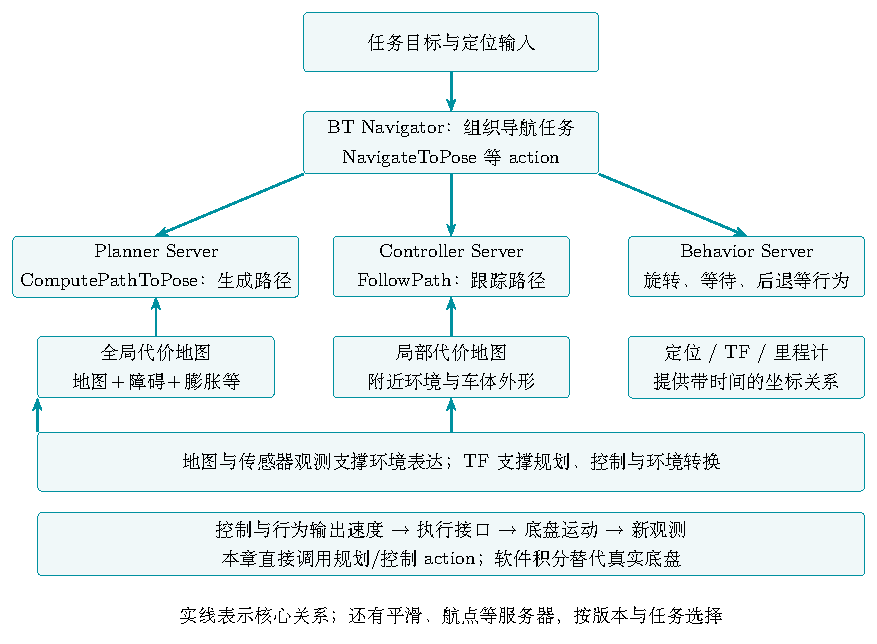
\includegraphics[width=.94\textwidth]{nav_framework_revised.pdf}
\caption{Nav2 的核心调用与数据关系；并非所有项目都只启动这几个服务器}
\label{fig:I_nav-1}
\end{figure}

先别急着给哨兵装手机，我们把刚才的六样东西对上号。[1]是记录场地的\textbf{地图（Map）}，它还要经过障碍更新、外形与通行余量等处理，才成为全局代价地图（Global Costmap）。[2]相当于整个导航系统，其中负责找路的是\textbf{规划器（Planner）}。[3]是\textbf{定位（Localization）}，其结果通过带时间的位姿、TF 等接口传给其他模块；TF 是坐标关系，自己不会凭空算出位置。[4]对应不断更新的\textbf{局部代价地图（Local Costmap）}。[5]对应\textbf{控制器（Controller）}，根据路径、位姿和附近障碍算出速度。[6]则是\textbf{恢复（Recovery）}策略，由任务逻辑决定什么时候等、什么时候重试，以及什么时候向上层报告失败。

不过，手机“信号不好”只是帮助记忆的类比。真实机器人可能是 TF 缺失、观测过期、没有可行控制或长期不前进，处理方式各不相同，不能一律先倒车再说。我们先定位，给规划器当前位置和目标；规划器给出路径，控制器跟踪，新的障碍进入代价地图后还可能触发重规划。这几个模块一直交换最新数据，才形成导航闭环。

\begin{example}\label{ex:nav-overview}
这章的小项目在本卷的 \texttt{examples/navigation/navigation-lab-demo}。首先在 Ubuntu 22.04 的 Humble 环境安装依赖，再进入项目。下面的路径是仓库位置示例，换成你自己的；使用 Distrobox 时，先进入已安装 Humble 的 Ubuntu 22.04 容器；示例容器名换成你自己的，原生 Ubuntu 用户跳过这一步。
\begin{tbash}
distrobox enter ubuntu2204
bash
source /opt/ros/humble/setup.bash
sudo apt-get install --no-install-recommends \
  ros-humble-navigation2 ros-humble-nav2-bringup \
  libpcl-dev cmake g++ python3-numpy python3-scipy \
  python3-matplotlib python3-yaml fonts-wqy-zenhei
cd /home/mijiao/Apps/Tutorial4New/02-专项技术栈/\
examples/navigation/navigation-lab-demo
export ROS_DOMAIN_ID=188
export ROS_LOCALHOST_ONLY=1
\end{tbash}
本章代码与配置使用 Humble 的 Nav2 接口，PCL 由系统的 libpcl-dev 提供。两终端需要同一套环境与 Domain ID；188 是演示选择，若本机已有项目使用它就换一个空闲值。

我们用生成的小地图，让真实 Nav2 服务器规划、控制，再由软件积分速度，观察机器人是否真的沿路前进。地图、TF、最短路和恢复的代码会在相应小节依次展开，完整调用在\ref{sec:nav-real}节。
\end{example}
\begin{exercise}\label{ex:nav-chain}
已有路径却没有速度输出，先查哪一段？如果连当前位置都拿不到，为什么反复点“重新规划”通常没用？画出你要检查的两个数据链。
\end{exercise}

\subsubsection{先把坐标关系接起来}
我们上一章让云台转到了某个角度，导航现在要回答“小哨兵在场地哪里”。在 ROS 中，变换（Transform）描述两个坐标系（Frame）的相对平移和旋转；一组有父子关系的变换就组成 TF 树。车体、雷达、相机都有自己的坐标系，查询一条连通路径，才能把某个雷达点换算到地图里。

\begin{figure}[H]
\centering
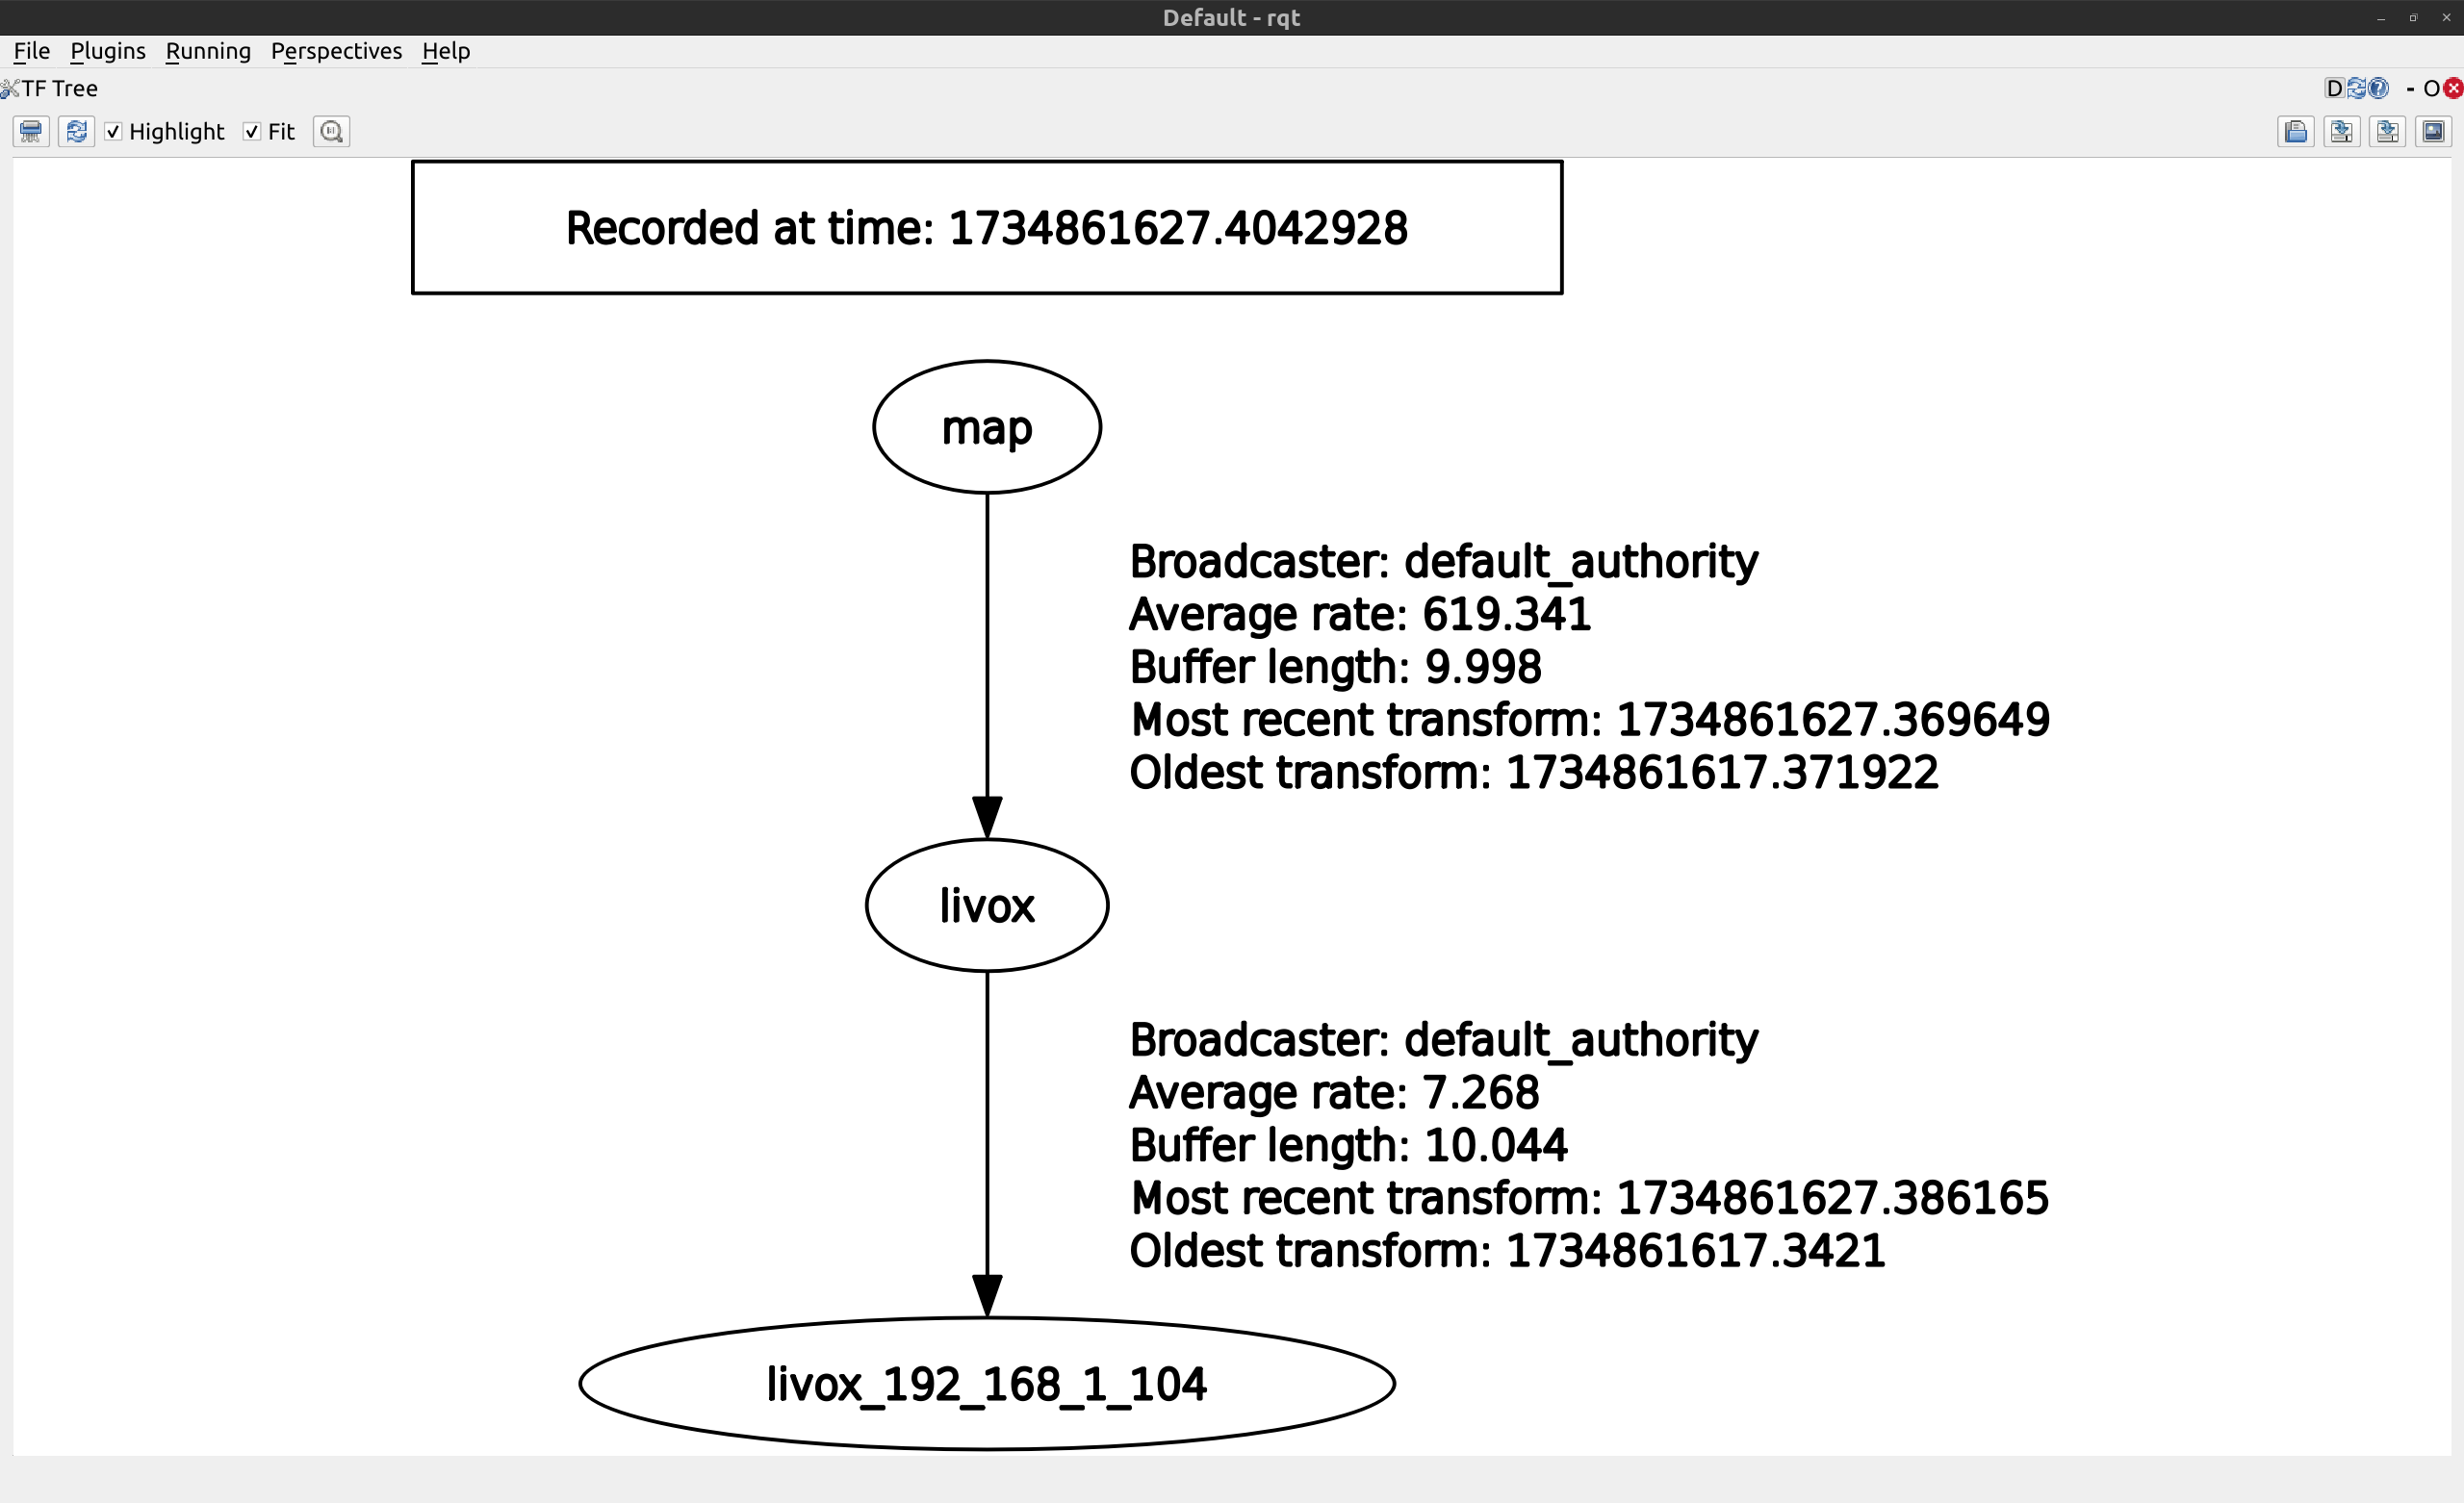
\includegraphics[width=.8\textwidth]{tf树_revised.png}
\caption{原项目的真实 TF 截图，记录 map、livox 与设备坐标系；图中的时间和频率保留原值，不能当成本章实验结果}
\label{fig:I_nav-2}
\end{figure}

名字通常用 \texttt{map}、\texttt{odom}、\texttt{base\_link}、\texttt{camera\_link}、\texttt{laser\_link}。它们是坐标系名称，开头不要加话题名那样的斜杠。图\ref{fig:I_nav-2}是原项目自定义关系的例子；想接入常见的移动机器人导航链，我们更常采用图\ref{fig:I_nav-3}的约定。
\begin{figure}[H]
\centering
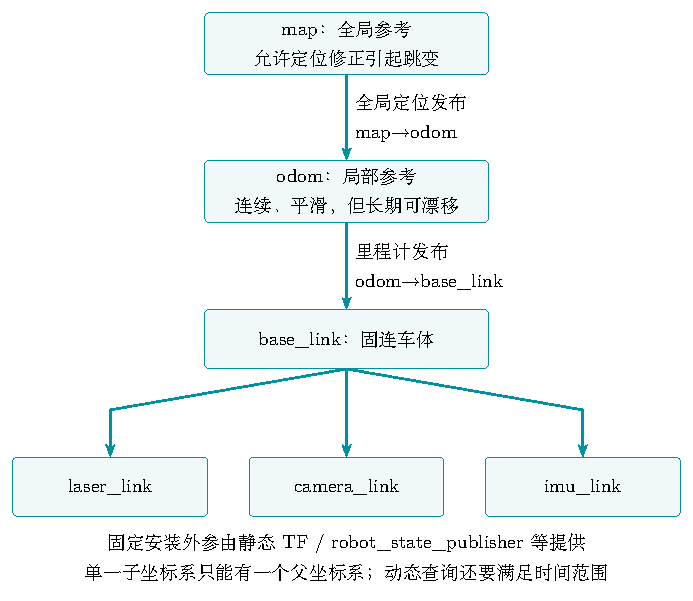
\includegraphics[width=.89\textwidth]{nav_frames_revised.pdf}
\caption{REP-105 的常见地图、里程计和车体关系；每个子坐标系只有一个父坐标系}
\label{fig:I_nav-3}
\end{figure}

\texttt{odom} 要让短时间的位置变化平滑、连续，即使走久了会漂；\texttt{map} 要对齐全局场地，定位修正时允许跳变；\texttt{base\_link} 固连车体。通常里程计发布 \texttt{odom→base\_link}，全局定位发布 \texttt{map→odom}，安装外参发布车体到传感器的固定变换。不要让两个节点抢着发布同一个子坐标系，不然哨兵可能没动，坐标先吵起来了。各坐标系的职责可对照\href{https://github.com/ros-infrastructure/rep/blob/master/rep-0105.rst}{REP-105 原文}。

\begin{example}
先做一条最简单的静态变换。终端一保持运行，终端二查询：
\begin{tbash}
# 终端一；只用独立演示坐标系
ros2 run tf2_ros static_transform_publisher \
  --x 1 --y 0 --z 0 --yaw 0 --pitch 0 --roll 0 \
  --frame-id demo_map --child-frame-id demo_base
# 终端二
ros2 run tf2_ros tf2_echo demo_map demo_base
\end{tbash}
稍等发现完成，应看到平移 $(1,0,0)$ 和零旋转。停止终端一后把 x 改为 2，再启动同一个发布程序，核对新的平移。不要同时启动两份发布者。
\end{example}

\begin{example}
一条边会查了，我们再查询两条边合成后的结果。\texttt{tf\_demo.py} 使用真实 tf2 Buffer 存入独立静态变换：第一条平移 $(1,2)$、旋转 $90^\circ$；第二条在父坐标系里沿 x 平移 2。代码完整如下：
\lstinputlisting[language=Python,basicstyle=\footnotesize\ttfamily]{examples/navigation/navigation-lab-demo/tf_demo.py}
\begin{tbash}
python3 tf_demo.py
\end{tbash}
输出约为 \texttt{xy: [1,4]}，缺失分支是 \texttt{LookupException}。为什么不是 $(3,2)$？因为第二条的 x 轴已经转向了地图的 y 轴。TF 连通还不够，动态变换也要覆盖查询时间；查旧时刻或未来时刻时出现外推异常，要先检查时间戳、时钟和缓存，不能靠把所有变换设为静态解决。
\end{example}
\begin{exercise}\label{ex:nav-tf}
完成 x=1 与 x=2 的命令实验，然后把 \texttt{tf\_demo.py} 第一条旋转改为零，预测并核对合成结果。解释真实 map→odom 为何不能长期用一个固定值代替。
\end{exercise}
\begin{conclusion}
地图负责全局一致，里程计负责局部连续，车体负责固定参考。位置可用要同时满足树连通、时间可查、单位与方向正确。TF 是这些关系的传递工具，定位算法才负责估计它们。
\end{conclusion}

\subsubsection{定位、建图和融合到底在忙什么}
导航里常听到 \textbf{SLAM（Simultaneous Localization and Mapping，同时定位与建图）}，简称 SM（不是）。定位可以在已有地图上匹配当前位置；SLAM 则在未知环境中同时估计自己的运动和地图，所以“所有定位都必须先有地图”并不成立。

可怜的小哨兵在场馆里通常没有可直接使用的 GPS，只好看周围的墙、柱子，读车轮和 IMU。激光雷达发射光并接收返回信号，测距后结合扫描角度得到点，有的还提供回波强度。将当前扫描与已有地图或局部子地图对齐，再结合雷达到车体的外参，就能估计车体位置。三维方法如 ICP、NDT，二维方法如基于栅格地图的 AMCL，各有适用条件；三维保留了高度信息，不意味着任何场景都一定更准确，精度和耗时还取决于几何、噪声、初值与实现。

局部匹配通常只看附近或最近的地图，让运动估计及时更新；全局重定位则扩大搜索范围，处理刚上电不知道在哪、位置已经明显不对等情况。不过，重定位不是“清空 TF，再把车体位置归零”。我们要用新的全局估计修正 map→odom，让 odom→base\_link 继续平滑，控制器才不会突然把定位修正当成底盘瞬移。

\begin{example}
设里程计认为车体在 $(2,0.5)$，地图匹配认为它在 $(2.3,0.5)$。按照变换相乘关系，
\[
T_{map,base}=T_{map,odom}T_{odom,base},\qquad
T_{map,odom}=T_{map,base}T_{odom,base}^{-1}.
\]
我们用 \texttt{localization.py} 跑一下这个修正，也顺便看看长走廊为什么容易让雷达迷路。
\lstinputlisting[language=Python,basicstyle=\footnotesize\ttfamily]{examples/navigation/navigation-lab-demo/localization.py}
\begin{tbash}
python3 localization.py
\end{tbash}
第一次 map→odom 的平移是 $(0.3,0)$；全局估计改为 $(2.2,0.5)$ 后修正变成 $(0.2,0)$，而里程计坐标仍是 $(2,0.5)$。两面沿 x 无限延伸的墙只约束横向，代码里的法向量矩阵特征值是 0 和 2，沿 x 移动 100 m 仍产生零墙面残差。这是几何退化的极简演示：实际走廊如果能看到端点、柱子等特征，纵向仍可能受到约束，不能把这两个数当成真实雷达定位误差。
\end{example}
\begin{exercise}\label{ex:nav-localization}
地图估计改成 $(1.8,0.7)$，计算新的 map→odom 平移。再给墙面约束增加法向量 $(1,0)$，运行查看新的特征值，说明它补上了哪个方向的信息。
\end{exercise}

轮式里程计把车轮运动累加起来，打滑会积累误差；IMU（Inertial Measurement Unit，惯性测量单元）测角速度和比力，要处理重力、偏置、安装方向与积分漂移，不能把读出的加速度直接加到地图坐标上。视觉里程计（Visual Odometry，VO）利用图像特征或像素变化估计运动，单目尺度、光照、遮挡、纹理都可能影响结果，也没有一个“视觉精度一定比激光低”的通用排名。

所以我们让传感器互相补位：轮子短时间走得连贯，地图匹配给全局修正，IMU 提供较快的运动信息。但“融合”也不是把三个坐标平均一下，外参、时间同步、噪声和退化条件都要先说清楚。否则融合的可能只是三份不同步的错误。第八章的滤波和第九章的几何优化，就是你继续深入时会用到的工具。

\begin{figure}[H]
\centering
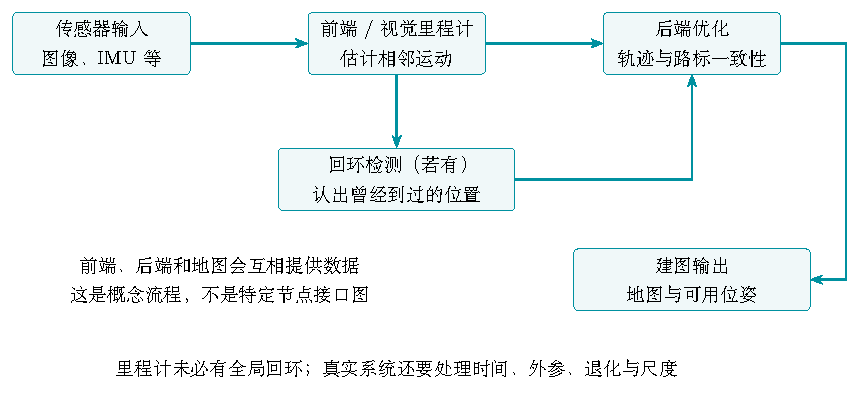
\includegraphics[width=.92\textwidth]{nav_slam_revised.pdf}
\caption{常见视觉 SLAM 的概念流程；回环可以修正累计误差，但不是所有里程计系统都有回环模块}
\label{fig:I_nav-4}
\end{figure}

从求解方式看，可以看到滤波与图优化两类思路，但具体系统经常组合使用。gmapping 使用粒子滤波；hector\_mapping 的核心是扫描匹配，不能一起塞进“都是滤波”的筐里。\href{https://index.ros.org/p/hector_mapping/}{hector\_mapping 的介绍}可以帮助核对这一点。Point-LIO 是激光惯性里程计的例子，\href{https://github.com/hku-mars/Point-LIO}{其原仓库}强调点时间戳、雷达与 IMU 同步、外参和 IMU 量程；原版提供的是 ROS 1 构建流程，接 ROS2 Humble 时还要核对实际采用的移植版本。这里没有把它装上就宣布“小哨兵会定位了”，本章先把输入输出和故障原因对上。
\begin{exercise}\label{ex:nav-fusion}
一份雷达数据落后 IMU 0.1 s，车体以 1 m/s 平移。仅考虑这个时间差，两份数据对应的位置会相差多少？再分别给出轮子打滑、白墙缺纹理和长走廊中的一个排查方向。
\end{exercise}
\begin{conclusion}
已有地图上的定位、连续运动估计和同时建图承担不同任务。回环是再次认出到过的地方并施加一致性约束，既可能纠正轨迹，也可能纠正地图；它不是凭空把所有误差清零。先问清传感器提供什么、哪个方向可观测，再选择融合或优化方法。
\end{conclusion}

\subsubsection{先把点云收拾一下}
导航需要地图。小哨兵还没学会飞行，我们先用二维导航表达，但 z、roll、pitch 仍会影响坡道、车体高度和传感器投影。地图通常可以从三维点云处理得到，也可以直接使用二维扫描建图。激光测到的主要是可见表面，没看到的地方不能自动当成空地。

首先，近处点云太密，全部计算容易变成“三帧电竞”，这时候可以用\textbf{体素下采样（Voxel Grid）}。PCL 的 VoxelGrid 把同一体素内的点合成\textbf{质心}，不是固定的体素几何中心。叶子尺寸越大，点越少，细小障碍也更可能被抹掉；不要只盯着帧率。

然后，用\textbf{直通滤波（Pass Through）}留下某个坐标范围。z 范围要先统一到合适坐标系，再根据车体可碰撞高度选择。雷达装在车顶时，“z 大于 0.5”未必就是离地 0.5 m；横梁、桌面等也可能让车体过不去，不能因为点在某个高度之外就宣判安全。

\textbf{统计离群点移除（Statistical Outlier Removal，SOR）}则计算点到 K 个近邻的平均距离，以全局均值加标准差倍数作阈值。这是对邻域平均距离分布的假设，不是“所有点坐标都符合高斯分布”。稀疏的真实障碍也可能被误删，所以换场地、换密度时要看滤前滤后。

\begin{example}
\texttt{point\_filters.cpp} 自己生成两组小点云，不需要雷达。第一组只有两个点，让你看清质心；第二组放入 30 个近点、1 个远离群点和 1 个低点，分别观察直通与 SOR。
\lstinputlisting[language=C++,basicstyle=\footnotesize\ttfamily]{examples/navigation/navigation-lab-demo/point_filters.cpp}
完整构建配置是 \texttt{CMakeLists.txt}，这里同时启用 C 与 C++，兼容 PCL 依赖中可能出现的 C/MPI 目标。
\lstinputlisting[language=bash,basicstyle=\footnotesize\ttfamily]{examples/navigation/navigation-lab-demo/CMakeLists.txt}
\begin{tbash}
cmake -S . -B build
cmake --build build -j4
./build/point_filters
\end{tbash}
实测输出为质心 x=0.02、输入 32、直通后 31、统计过滤后 30。0.1 m 体素的中心 x 是 0.05，这就能直接区分“体素中心”和“点的质心”。PCL 的\href{https://pointclouds.org/documentation/tutorials/voxel_grid.html}{VoxelGrid 教程}与\href{https://pointclouds.org/documentation/tutorials/statistical_outlier.html}{SOR 教程}可查参数；网页版本可能更新，本例在 PCL 1.14.0 上实际编译运行。
\end{example}
\begin{exercise}\label{ex:nav-filter}
将两个点的 x 改为 0.01 和 0.09，先手算质心，再同步修改程序中的核对值并运行。若叶子尺寸改为 0.02，它们还在同一个体素吗？说明为什么不能为了让程序返回 0 就忽略真实输出。
\end{exercise}

最后还有地面提取。简单的 z 截取、平面拟合、法向量和聚类都能提供线索，但“最大聚类就是地板”“平的就是地板”都只是特定场景的假设。桌面也平，墙面也可能是最大一组点，我们还要结合高度、朝向、连续性与场地结构。原项目的法向量方法可以保留为工程选择，阈值与误删风险应通过真实地面和障碍样本验证，这部分放到卷三建图实验。

\subsubsection{把地图保存完整，再谈哪里能走}
现在，你拿到了某个时刻附近的点。要拼成完整地图，先用每一帧的位姿把它们变到共同坐标系，再处理动态物体、遮挡和误差，不能把传感器原坐标下的数组直接叠起来。三维地图常存为 PCD；二维栅格通常由 PGM/PNG 图片与 YAML 元数据共同表示。尽量保留无损图片，JPG 的压缩边缘可能影响障碍判定。

栅格索引 $(i,j)$ 对应的不是格角而是格心。设分辨率 r、地图原点 $(o_x,o_y)$ 和偏航 $\psi$，先得到局部格心，再旋转平移：
\[
\begin{bmatrix}x\\y\end{bmatrix}=
\begin{bmatrix}o_x\\o_y\end{bmatrix}+
\begin{bmatrix}\cos\psi&-\sin\psi\\\sin\psi&\cos\psi\end{bmatrix}
\begin{bmatrix}(i+0.5)r\\(j+0.5)r\end{bmatrix}.
\]
所以宽 W、高 H 格的地图覆盖 $Wr\times Hr$，只把图片缩放一下而不改元数据，场地就会被你偷偷放大或缩小。图像通常从顶部开始数行，而地图从较小 y 向上数；没有旋转时，第 v 行对应 $j=H-1-v$。

\begin{example}\label{ex:nav-grid-project}
我们把栅格换算、生成输入和找路放进同一个 \texttt{grid.py}。本小节先看 \texttt{cell\_center} 和生成 PGM/YAML 的部分；\texttt{shortest} 与 \texttt{plan} 在下一小节继续使用，所以这里给出完整文件，后面直接对照。
\lstinputlisting[language=Python,basicstyle=\footnotesize\ttfamily,firstline=1,lastline=43]{examples/navigation/navigation-lab-demo/grid.py}
\lstinputlisting[language=Python,basicstyle=\footnotesize\ttfamily,firstnumber=44,firstline=44]{examples/navigation/navigation-lab-demo/grid.py}
\begin{tbash}
python3 grid.py --output out/map
python3 -c 'from grid import cell_center; print(\
cell_center(10,20,.05,(0,0,0)))'
cat out/map/map.yaml
\end{tbash}
第二行得到 $(0.525,1.025)$ m。生成图固定 60×40 格、0.1 m/cell，也就是 6×4 m，黑色边框和中央矩形是人为障碍。保存时上下翻转，\texttt{map.yaml} 的内容如下，图片路径相对 YAML 所在目录解释：
\begin{tbash}
image: map.pgm
mode: trinary
resolution: 0.1
origin: [0.0, 0.0, 0.0]
negate: 0
occupied_thresh: 0.65
free_thresh: 0.25
\end{tbash}
这是三值地图模式：图像灰度经 negate 规则转换为占据概率，再按两个阈值分类。ROS 的占据栅格（OccupancyGrid）用 -1 表示未知、0～100 表示占据；Nav2 原始代价地图有另一套 0～255 的编码。未知不等于自由，两套数组也不能不转换就直接交换。
\end{example}
\begin{exercise}\label{ex:nav-map}
把原点改为 $(-2,-1)$，求同一个 $(10,20)$ 格心。如果改为原点 $(1,2)$、偏航 $90^\circ$、分辨率 0.1，求 $(2,3)$ 格心并用函数核对。40 行图片的第 0 行对应哪个地图 j？
\end{exercise}
\begin{note}
定位地图应保留可复核的几何信息。禁止通行区用导航约束表达，编辑前保留原始版本，再核对实际场地；把未知刷成白色只是骗过规划器，墙不会因为你修图就消失。
\end{note}

\subsubsection{给路径算代价，也给车留空间}
地图能帮助定位，但要找路，还需要代价地图（Costmap）：自由区域代价低，越靠近障碍代价越高，致命障碍不能通过。为了方便“掺点小料”，Nav2 用地图层（Layer）插件组合信息。静态层（Static Layer）接收已有地图，障碍层（Obstacle Layer）根据观测标记、清除障碍，体素层（Voxel Layer）可保留高度信息，膨胀层（Inflation Layer）在障碍周围生成代价分布，通常放在要膨胀的障碍层之后。

哨兵不是不计体积的理想质点，膨胀层因此堂堂登场。不过，调一个 inflation\_radius 就不代表完成了碰撞检查，还要正确配置车体轮廓（Footprint）或半径，并留出定位、离散化和控制误差的余量。KeepoutFilter 和 SpeedFilter 是代价地图过滤器，配置接口与普通 layer 有区别，分别表达禁止区和区域限速；区域限速不能替代底盘本身的速度上限。

全局代价地图供较大范围的规划，局部代价地图供附近控制；内容和更新速度由任务决定，不是固定的“三层对两层”。本项目已知一张静态地图，所以两张代价地图都使用静态层与膨胀层；没有伪装成雷达正实时扫描动态障碍。

\begin{example}
假设车速 v=2 m/s、可用制动减速度 a=1 m/s$^2$，理想制动距离为 $v^2/(2a)=2$ m；再加 0.2 s 的总延迟，至少多走 0.4 m。若机器人位于 4 m 方形局部窗口的正中心，正前方可见长度只有 2 m，这还没算余量就不够。窗口应覆盖预测、停车与观测需求，频率也要能在预算内完成，不是越快越好。

离线 \texttt{plan} 用障碍格心距离大于 margin 判断可通行，\texttt{--margin} 默认 0.35 m。它只是四邻接算法实验的模型，不是完整 Nav2 footprint 检查。运行 \texttt{python3 grid.py --margin 0.6 --output out/wide}，比较通道变窄后的路线；margin 大到起终点也被挡住时，代码明确返回无路。
\end{example}
\begin{exercise}\label{ex:nav-costmap}
速度保持 2 m/s、延迟仍为 0.2 s，将减速度改为 2 m/s$^2$，计算不含额外余量的前向距离需求。5 m 方形窗口的半宽够不够？再解释清空动态障碍层为什么不应清掉静态墙。
\end{exercise}
\begin{conclusion}
图片是地图输入，地图层组合成代价地图，外形检查与控制再决定运动是否可行。全局地图不能自动看到新障碍，局部地图也不能只靠扩大范围补救过期观测。配置外形、更新范围、延时和制动能力时，要把它们放在同一个量级里看。
\end{conclusion}

\subsubsection{现在终于可以找路了}
有了地图和定位，我们进入正题。Dijkstra 在非负边权图上，每次取累计代价最小的候选点向外扩展；普通广度优先搜索只有在各边等权时才能直接这样求最低代价。A* 则按 $f(n)=g(n)+h(n)$ 选候选点，其中 g 是已经走过的代价，h 是到目标的估计。

本例的四邻接就是每格只连接上下左右四格。在 \texttt{grid.py} 的四邻接图里每步代价为 1，曼哈顿距离不高估剩余步数，并满足一致性，所以 A* 可以更有方向地找到同样最低代价的路线。若随手把 h 乘十，或者用了与边权不匹配的距离，就不能继续宣称最优。最少拐弯、最短距离、最快时间，也不是同一个优化目标；Nav2 插件的结果由代价与约束共同决定。
\begin{example}
先跑三顶点图，再对照上面的完整 \texttt{shortest}：
\begin{tpython}
from grid import shortest
graph = {"A": [("B", 1), ("C", 5)],
         "B": [("C", 2)], "C": []}
print(shortest(graph.__getitem__, "A", "C"))
\end{tpython}
输出路径 A→B→C、代价 3。返回值还记录取出的候选点次数，用于比较这份实现的搜索工作量。再运行：
\begin{tbash}
python3 grid.py --output out/map
python3 grid.py --blocked --output out/blocked
\end{tbash}
默认地图中两算法总代价均为 70、路径均有 71 格；本实现 Dijkstra 扩展 1304 次，A* 扩展 914 次，数量也受相同代价时的取点顺序影响。\texttt{--blocked} 加入一面贯穿地图的墙，二者都返回空路径和 \texttt{cost: null}。返回“无路”才是合理结果，不能为了完成任务穿墙。
\end{example}
\begin{exercise}\label{ex:nav-search}
将三顶点图 A→C 改为 2，运行核对；再看默认栅格，解释为什么 A* 与 Dijkstra 同代价却可能取到不同路线。若边权为负，程序怎样处理？
\end{exercise}

\subsubsection{让规划出的路径真的变成运动}\label{sec:nav-real}
如果只有规划器会怎么样？想象你在游戏里给角色指定了远处目标：
\begin{figure}[H]
\centering
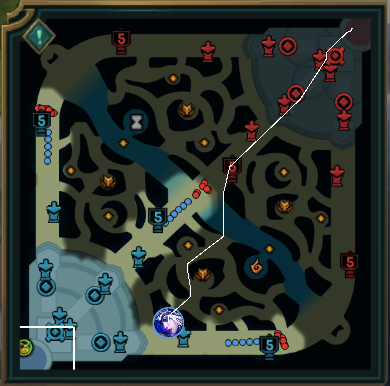
\includegraphics[width=.48\textwidth]{英雄联盟_revised.png}
\caption{原游戏小地图，用来类比全局路线；截图本身不能证明游戏使用了 A*}
\label{fig:I_nav-5}
\end{figure}
规划时没看到的移动目标可能突然挡路，只有路线还不够。回到缺德地图，你这位车手对应控制器，地图只告诉你怎么绕到目的地，你还要根据视野和车的能力决定眼下怎样转向、减速。Nav2 控制器通常输出 Twist 或 TwistStamped 速度，而不是直接替底盘算电机电流；电控执行接口还要在卷三接起来。

DWA、TEB 是常见的局部规划思路，但不能看到 Nav2 就默认它们正在运行。本章在 Humble 中明确选 Navfn 规划器和调节纯追踪（Regulated Pure Pursuit，RPP）控制器。RPP 根据前方追踪点与几何关系跟踪路径，同时调节速度并检查碰撞；它不是任意动态障碍下都能自行绕路的控制器。算法与参数可对照\href{https://github.com/ros-navigation/navigation2/tree/humble/nav2_regulated_pure_pursuit_controller}{Humble 的 RPP 说明}，实际插件以加载日志与配置为准。

\begin{example}\label{ex:nav-real-run}
首先看 \texttt{params.yaml}。\texttt{GridBased}、\texttt{FollowPath} 是我们给插件实例起的名字，后面的 action 请求要用相同 ID。控制频率 20 Hz；局部窗口 4×4 m；车体用半径 0.15 m 的圆；膨胀半径 0.35 m。配置使用 Humble 的 Twist 输出，没有速度平滑器、真实传感器或碰撞监控器。
\lstinputlisting[language=bash,basicstyle=\footnotesize\ttfamily,firstline=1,lastline=36]{examples/navigation/navigation-lab-demo/params.yaml}
接下来是两张代价地图的完整配置：
\lstinputlisting[language=bash,basicstyle=\footnotesize\ttfamily,firstnumber=37,firstline=37]{examples/navigation/navigation-lab-demo/params.yaml}

然后，\texttt{sim.py} 接收实际 \texttt{cmd\_vel}，用单调时钟的实际间隔积分平面运动，发布 odom 和 TF。固定 map→odom 为单位变换，是因为软件模型没有定位漂移；它明确替代了本实验的定位输入，不能搬到真实哨兵上当定位系统。
\lstinputlisting[language=Python,basicstyle=\footnotesize\ttfamily]{examples/navigation/navigation-lab-demo/sim.py}
该模型忽略惯性、打滑和碰撞动力学，断流 0.5 s 后只让软件停止积分。导航避障取决于实际代价地图和控制器检查，最后还应检查保存轨迹是否与障碍相交。

\texttt{lab.launch.py} 把 map\_server、planner\_server、controller\_server、生命周期管理器和软件模型一起启动。生命周期管理器负责配置、激活服务器，\texttt{map} 启动参数替换地图文件位置；整个示例不需要新建 ROS 包。
\lstinputlisting[language=Python,basicstyle=\footnotesize\ttfamily]{examples/navigation/navigation-lab-demo/lab.launch.py}

最后，\texttt{client.py} 等服务器真正激活，再调用 \texttt{ComputePathToPose}，成功后才调用 \texttt{FollowPath}。它订阅并保存真实服务器输出的速度和软件 odom，超时会请求取消，失败则保留 action 状态。Humble 的这两个 action 结果没有 \texttt{error\_code} 字段；成功与否用状态判断，具体失败原因从启动终端日志定位。进度检查器由服务器的 \texttt{progress\_checker\_plugin} 指定，不在 FollowPath 请求中另设 ID。
\lstinputlisting[language=Python,basicstyle=\footnotesize\ttfamily,firstline=1,lastline=50]{examples/navigation/navigation-lab-demo/client.py}
\lstinputlisting[language=Python,basicstyle=\footnotesize\ttfamily,firstnumber=52,firstline=52]{examples/navigation/navigation-lab-demo/client.py}
两个终端都进入项目、加载同一 ROS 环境和隔离 Domain，然后运行：
\begin{tbash}
# 终端一：先生成地图，launch终端保持运行
python3 grid.py --output out/map
ros2 launch "$PWD/lab.launch.py"
# 终端二
python3 client.py --output out/nav2
ros2 topic type /cmd_vel
ros2 param get planner_server GridBased.plugin
ros2 param get controller_server FollowPath.plugin
ros2 run tf2_ros tf2_echo map base_link
\end{tbash}
看到 \texttt{Managed nodes are active} 后地图与服务器已经激活；刚启动时短暂的“等待 TF”与一直超时不是同一种情况。客户端也会检查生命周期，避免“action 能连上，地图却还没准备好”的竞争。

正常完成时，规划状态和跟踪状态应均为 4（Succeeded），最终位置误差应在配置的 0.1 m 容差附近；路径点数以当前规划结果为准。具体 odom/速度样本数随运行调度变化，以你保存的 \texttt{result.json} 为准。本例应能观测到 60×40 的 map 和 global costmap；map 的值是 0/100，原始 costmap 中还有 253、254 和一系列膨胀代价，能看出它们不是同一数组。
\end{example}
\begin{exercise}\label{ex:nav-run}
实际启动该闭环，保存结果，核对插件 ID、cmd\_vel 类型、路径长度和最终位置误差。然后运行 \texttt{python3 client.py --blocked-goal --output out/nav2-blocked}，目标落在障碍中；它有没有继续调用控制器？从日志指出中断位置。
\end{exercise}

\begin{example}
现在把保存的数据画出来。\texttt{plot.py} 只读上面那次结果，不另造一条“看上去很成功”的轨迹。
\lstinputlisting[language=Python,basicstyle=\footnotesize\ttfamily]{examples/navigation/navigation-lab-demo/plot.py}
\begin{tbash}
python3 plot.py --map out/map --nav2 out/nav2 \
  --output out/navigation.pdf
\end{tbash}
默认字体使用依赖里的文泉驿，\texttt{--font} 可换成你机器上的中文字库；教材插图使用 Fandol 与其他章协调。左图看离线格心路线，右图看真实 Navfn 路径与软件轨迹，两边的模型与代价不同，不要求路径点一一重合。
\begin{figure}[H]
\centering
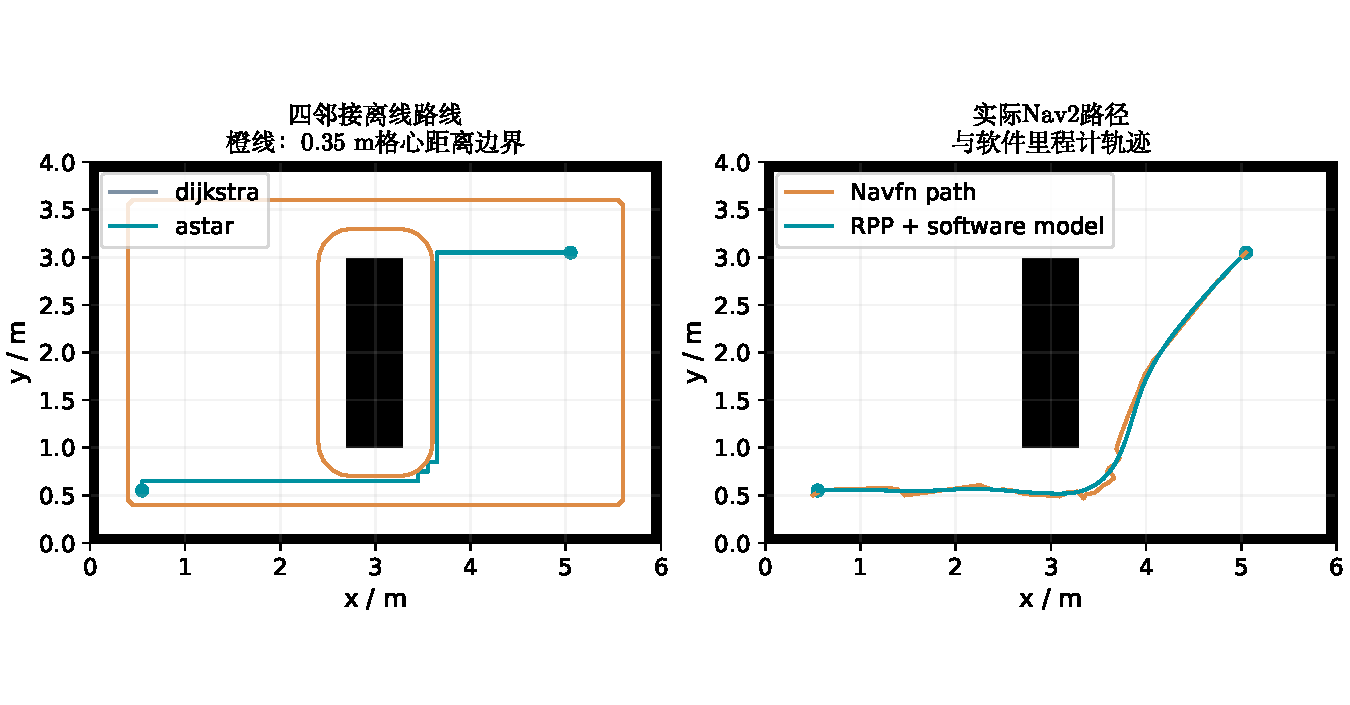
\includegraphics[width=.96\textwidth]{nav_paths_revised.pdf}
\caption{一组保存数据：四邻接离线路线与 Nav2 的规划、跟踪结果}
\label{fig:nav-paths}
\end{figure}
\end{example}
\begin{exercise}\label{ex:nav-plot}
把 \texttt{desired\_linear\_vel} 改为 0.3，停止终端一并重新启动，从同一初始位置跑到同一目标，保存到另一个输出目录。比较实际速度峰值与到达时长；说明为什么不能只改图上的标签就声称已经验证了慢速运行。
\end{exercise}
\begin{note}
项目输出目录用于保存当前实验，重复运行同一路径会覆盖数据。终端一 Ctrl+C 结束本项目；演示没有连接真实底盘，不应把这些配置直接启动在正在运动的机器人环境里。本章的圆形模型与静态场地软件验证，不能证明真实底盘制动、雷达覆盖或动态避障能力。
\end{note}

\subsubsection{失败以后，别让哨兵无限重试}
规划无路、控制无有效速度、进度长期不变时，任务需要选择恢复。清空过时障碍信息、等障碍离开、重新规划、旋转或后退都有用途，但要针对原因：清地图不能清掉真实墙，倒车也要先核对后方可行空间；TF 丢失时更应该修复数据链，而不是盲目转圈。

Nav2 的行为树（Behavior Tree，BT）用任务节点和控制节点组织流程。执行节点调用规划、控制或行为服务器；顺序（Sequence）按顺序执行，失败就停；选择（Fallback）只在当前分支失败时才试下一分支。节点返回 Success、Failure 或 Running；Running 表示还没完成，必须向上传递，不能一边跟踪路径一边误启动恢复。具体还有带记忆、响应式等控制节点，名称相似也要看执行语义。

\begin{example}
\texttt{bt.py} 是可以逐 tick 运行的等价教学模拟器，\texttt{Control} 实现带记忆的顺序/选择节点，\texttt{Recovery} 在导航失败后轮流清理、等待，成功才重试导航，最多完成两次恢复；恢复分支自己失败则立即退出。这与实际 Nav2 的\href{https://docs.nav2.org/rolling/configuration_and_development/configuration_guide/core_servers/bt_plugins/controls/RecoveryNode/}{RecoveryNode 重试职责}相对应，但本文件不是 Nav2 插件，也没有真的删代价地图。
\lstinputlisting[language=Python,basicstyle=\footnotesize\ttfamily,firstline=1,lastline=35]{examples/navigation/navigation-lab-demo/bt.py}
\lstinputlisting[language=Python,basicstyle=\footnotesize\ttfamily,firstnumber=36,firstline=36]{examples/navigation/navigation-lab-demo/bt.py}
\begin{tbash}
python3 bt.py
python3 bt.py --fail
python3 bt.py --stuck
\end{tbash}
默认日志依次为导航失败、清理成功、导航失败、等待 Running、等待成功、导航成功，最终重试计数为 2。\texttt{--fail} 让导航持续失败，恢复两次后结束为 Failure；\texttt{--stuck} 让等待一直 Running，十次 tick 后外层预算输出 Timeout。这个 tick 预算不是秒级实时保证，真实任务还要结合时钟期限和取消逻辑。

要直接核对 Fallback 的 Running 传播，可以在项目目录执行：
\begin{tpython}
from bt import Control, Script, RUNNING, SUCCESS
log = []
root = Control([Script("follow", [RUNNING], log),
                Script("recover", [SUCCESS], log)], sequence=False)
print(root.tick(), log)
\end{tpython}
只应记录 \texttt{follow}，不会调用 \texttt{recover}。真实导航的完整 BT XML 应结合已安装版本查看，BT Navigator 组织的不止规划与控制，还可以调用行为、平滑等服务，不能把导航软件永久写成“一大三小”。
\end{example}
\begin{exercise}\label{ex:nav-bt}
用 \texttt{Control} 分别核对两个分支均 Failure 的 Fallback、第一分支 Running 的 Sequence。再运行三种恢复序列，记录每次 tick 的返回值，解释恢复次数和 tick 预算各自限制什么。
\end{exercise}
\begin{conclusion}
规划器说“路在哪”，控制器说“现在怎么动”，恢复逻辑说“失败后怎么办”。恢复次数要有限，Running 要有上层时间预算，最终失败要能通知任务决策；让哨兵原地重试到比赛结束，日志可能挺努力，任务还是没完成。
\end{conclusion}


\section{本章小结}
导航把“我在哪、哪里能走、怎样到达、失败怎么办”连接成闭环。TF 统一坐标，地图表示环境，代价地图加入障碍与外形约束，规划器生成路径，控制器跟踪路径并持续处理局部变化。应熟练定位断点和读参数；SLAM、控制器插件与行为树扩展按具体方向深入。

\begin{problemset}
\item 基础：系统已有全局路径，但控制器未输出速度，应先检查规划器还是控制链？
\item 基础：map、odom、base\_link 的典型作用是什么？
\item 基础：分辨率 0.1 m/cell、原点为 (1,2)、无旋转，索引 (2,3) 的格心在哪里？
\item 基础：静态层、障碍层、膨胀层分别承担什么？
\item 基础：A-B 代价 2、B-C 代价 2、A-C 代价 5，Dijkstra 选择哪条路线？
\item 基础：Fallback 的第一个子项返回 Running，是否立即执行下一个子项？
\item 提高：机器人速度 2 m/s、可用制动减速度 1 m/s²，忽略其它因素的制动距离是多少？为什么局部地图边界不能小于它？
\item 实践：修改本章最短路程序，使 A-B=4、B-C=4、A-C=5，运行并记录到 C 的距离。
\end{problemset}

\section{本章验收}
\begin{enumerate}
    \item 对照实际 Nav2 配置或离线日志，展示规划器、控制器与代价地图的输入输出，解释一个故障的排查路径。
    \item 演示独立 TF 树查询，说明 map、odom、base\_link 的关系；在模拟环境中展示一处变换缺失的表现。
    \item 按检查者给定的失败序列演示行为树或等价模拟器，展示至少两种恢复分支、重试上限和最终失败出口。
\end{enumerate}


\chapter*{卷二小结}
\addcontentsline{toc}{chapter}{卷二小结}
本卷为自瞄、导航、决策和雷达四个方向提供专项技术基础（含共用的图像处理、深度学习与 CUDA）。
赛场链路、工程准则与任务级案例见 \textbf{卷三 · RM 视觉概述}。

% 统一题解放在卷二全文末尾，题目仍保留在原章。
\chapter*{参考题解}
\addcontentsline{toc}{chapter}{参考题解}
\markboth{参考题解}{参考题解}
% 卷二完整题解；由 main.tex 在全文末尾载入。
\begingroup
\setlength{\emergencystretch}{3em}

先完成题目，再来核对。下面按正文顺序整理随堂练习与章末题；两套编号分开，例如“随堂练习 1.1”与“第一章章末第 1 题”不是同一道题。
操作题给出步骤、预期结果和判断依据；依赖设备、软件版本或实验数据的数值，以实际记录为准。
本章验收用于现场考核，不另列一份可以照抄的验收答案。

\section*{第一章：ROS2 基础}
\phantomsection
\addcontentsline{toc}{section}{第一章题解：ROS2 基础}
\subsubsection*{随堂练习}

\paragraph*{随堂练习 \ref{ex:v2-ros-setup}}
\begin{solution}
talker 属于 \texttt{demo\_nodes\_cpp}。加载当前发行版环境后，可执行：
\begin{tbash}
ros2 pkg executables demo_nodes_cpp
ros2 run --help
ros2 run demo_nodes_cpp talker
\end{tbash}
前两条分别确认包中的可执行程序与启动语法，第三条启动发布节点。按 Ctrl+C 结束。
\end{solution}

\paragraph*{随堂练习 \ref{ex:v2-ros-graph}}
\begin{solution}
在只启动一个示例 talker 的环境中，\texttt{/chatter} 类型为 \texttt{std\_msgs/msg/String}，发布者数量通常为 1。
\begin{tbash}
ros2 topic info /chatter
ros2 node list
\end{tbash}
停止 talker 后等待发现信息更新，发布者数量应变为 0，或话题不再列出；如果 echo 等订阅者仍在运行，话题可能仍可见。节点是功能实体，话题是通信通道，不能用“还能查到话题”判断发布节点是否存活。
\end{solution}


\paragraph*{随堂练习 \ref{ex:v2-ros-qos}}
\begin{solution}
可靠发布者能够满足 best\_effort 订阅者的要求，所以可以通信。发布端和订阅端按“提供的策略是否满足要求”匹配，不要求每项值都相等。分别运行：
\begin{tbash}
# 终端一
ros2 topic pub /qos_demo std_msgs/msg/String "{data: hello}" --rate 1 --qos-reliability reliable
# 终端二
ros2 topic echo /qos_demo std_msgs/msg/String --qos-reliability best_effort --once
\end{tbash}
应收到 hello。这里只改变可靠性，其他策略保持兼容；不能由这个实验推断任何 QoS 组合都能通信。
\end{solution}

\paragraph*{随堂练习 \ref{ex:v2-ros-message}}
\begin{solution}
在 \texttt{my\_msgs/msg/My.msg} 末尾加入 \texttt{float64 distance}，保存后回到工作空间根目录：
\begin{tbash}
cd ~/ros2_ws
colcon build --packages-select my_msgs
source install/setup.bash
ros2 interface show my_msgs/msg/My
\end{tbash}
应看到新增字段。若节点要访问该字段，再重新构建依赖它的包，例如执行 \texttt{colcon build --packages-up-to my\_package}。单位约定为米，应同时写在接口注释或文档里。
\end{solution}

\paragraph*{随堂练习 \ref{ex:v2-ros-timer}}
\begin{solution}
将构造函数中的间隔改为 \texttt{std::chrono::milliseconds(500)}，重新构建、加载环境并重启节点。在另一个已加载环境的终端执行：
\begin{tbash}
ros2 topic hz /timer_
\end{tbash}
理论频率为 2 Hz，调度和观测窗口会造成小幅波动。计数器只表示回调执行次数；时间戳表示特定时钟下的事件时间。间隔改变后，一次计数不再等于一秒，不能用计数器代替时间戳。
\end{solution}

\paragraph*{随堂练习 \ref{ex:v2-ros-service}}
\begin{solution}
服务端运行时查询：
\begin{tbash}
ros2 service list -t
ros2 interface show example_interfaces/srv/AddTwoInts
\end{tbash}
请求包含两个 \texttt{int64} 字段 a、b，响应包含 \texttt{int64 sum}；接口中的三条短横线分隔请求和响应。服务对应一次请求与一次响应，话题用于按发布端节奏持续传递数据，两者用途不同。
\end{solution}


\paragraph*{随堂练习 \ref{ex:v2-ros-reply}}
\begin{solution}
receive 与 send 都使用 \texttt{std\_msgs/msg/String}。先保持 \texttt{ros2 topic echo /send} 运行，再在另一终端发送：
\begin{tbash}
ros2 topic pub --once /receive std_msgs/msg/String "{data: armor_found}"
\end{tbash}
应收到 \texttt{I can hear:armor\_found}。停止节点后，原命令可能等待订阅者；加 \nolinkurl{--wait-matching-subscriptions} 并设为 0，可以在没有订阅者时也发送一次，但不会收到回复。CLI 打印 publishing 只说明发布端执行了发送，处理是否发生要由回调日志、响应消息等证据确认。
\end{solution}

\paragraph*{随堂练习 \ref{ex:v2-ros-domain}}
\begin{solution}
域不同的两个节点不能按普通 DDS 发现互相通信；统一为 42 后应恢复收发。两端都先停止节点，再设置相同的 \texttt{ROS\_DOMAIN\_ID} 和发现范围，执行 \texttt{ros2 daemon stop} 并重新启动。恢复默认实验环境时停止节点、unset \texttt{ROS\_DOMAIN\_ID}、\texttt{ROS\_LOCALHOST\_ONLY}、\nolinkurl{ROS_AUTOMATIC_DISCOVERY_RANGE} 和 \texttt{ROS\_STATIC\_PEERS}，停止 daemon 后重新运行；持久写入启动文件的设置也需删除或更改。域隔离实验须排除同名遗留发布者。
\end{solution}

\paragraph*{随堂练习 \ref{ex:v2-ros-ament}}
\begin{solution}
启动系统通常从安装索引查资源。检查 CMake 是否安装 launch/config 目录、是否重新构建，以及当前环境是否指向该工作空间。手动版本应包含：
\begin{tcode}
install(DIRECTORY launch config DESTINATION share/${PROJECT_NAME})
\end{tcode}
间隔函数改为 \texttt{milliseconds >= 10 \&\& milliseconds <= 500}；合法边界测试为 10 和 500，非法测试为 9 和 501。\Needspace{11\baselineskip}
保存后执行：
\begin{tbash}
cd ~/ros2_ws
colcon build --packages-select training_tools --cmake-args -DBUILD_TESTING=ON
source install/setup.bash
colcon test --packages-select training_tools
colcon test-result --verbose
ros2 pkg prefix training_tools
\end{tbash}
预期边界测试全部通过，包前缀指向当前工作空间的安装目录。
\end{solution}

\paragraph*{随堂练习 \ref{ex:v2-ros-launch}}
\begin{solution}
在 team 文件中将 observer 的 cmd 改成下面的列表，其余配置保持不变。嵌套列表把三个替换片段拼成同一个话题参数：
\begin{tpython}
cmd=['ros2', 'topic', 'echo',
     ['/', LaunchConfiguration('robot'), '/health'],
     'std_msgs/msg/String', '--once'],
\end{tpython}
重新构建、加载环境后运行：
\begin{tbash}
ros2 launch training_tools team.launch.py robot:=blue
\end{tbash}
应看到一条 team ready 消息及观测进程退出提示，heartbeat 继续运行。结束后再次启动：
\begin{tbash}
ros2 launch training_tools team.launch.py robot:=blue watch:=false
\end{tbash}
此时不启动 echo 进程。用另一个终端查询 \texttt{ros2 node list}、\texttt{ros2 topic info /blue/health}，应确认 heartbeat 发布者存在；查询命令本身可能产生临时观测节点，不能仅凭节点总数判断。
\end{solution}

\paragraph*{随堂练习 \ref{ex:v2-ros-log}}
\begin{solution}
定时器仍为 200 毫秒，所以理论消息频率是 5 Hz；alive 限流改成 1000 毫秒后约为 1 Hz。修改源码、重新构建、加载环境并重启后，用 \texttt{ros2 topic hz /status} 测量前者，按日志时间戳检查后者。调度、观测窗口和所用时钟会影响实测间隔。WARN 阈值仅隐藏 INFO/DEBUG 日志，发布逻辑仍运行，不会因此停止消息。
\end{solution}

\paragraph*{随堂练习 \ref{ex:v2-ros-ide}}
\begin{solution}
IDE 默认运行独立构建目录中的目标，\texttt{ros2 run} 根据已加载环境运行安装目录中的目标。仅执行 IDE Build 时，安装目录可能仍是旧程序。先去掉运行配置中的 \texttt{-p text:=from\_ide} 等文本覆盖，才能观察修改后的默认值；否则参数会掩盖源码默认值的变化。停止旧进程，然后执行：
\begin{tbash}
cd ~/ros2_ws
source /opt/ros/jazzy/setup.bash
colcon build --packages-select training_tools
source install/setup.bash
ros2 pkg prefix training_tools
ros2 run training_tools heartbeat
\end{tbash}
确认包路径属于当前工作空间，观察 /status 应得到 from\_debug。若仍是旧值，检查是否有其他发布者、参数覆盖、同名覆盖包，以及实际改动的源码路径。
\end{solution}

\subsubsection*{章末习题}

\paragraph*{第一章章末第 \ref{prob:v2-ros-1} 题}
\begin{solution}
包为 1，两个程序各启动一次时进程与节点各为 2；同一进程也可以包含多个节点。
\end{solution}

\paragraph*{第一章章末第 \ref{prob:v2-ros-2} 题}
\begin{solution}
加载 install/setup.bash；build 是中间构建结果，log 是日志。
\end{solution}

\paragraph*{第一章章末第 \ref{prob:v2-ros-3} 题}
\begin{solution}
不是，它表示历史队列深度；周期发布通常由定时器及回调执行情况决定。
\end{solution}

\paragraph*{第一章章末第 \ref{prob:v2-ros-4} 题}
\begin{solution}
类型为 \texttt{my\_msgs::msg::My}，包含头文件 \texttt{my\_msgs/msg/my.hpp}。
\end{solution}

\paragraph*{第一章章末第 \ref{prob:v2-ros-5} 题}
\begin{solution}
核对消息类型、命名空间、域标识、QoS 兼容性和终端环境；再确认节点存活、发布逻辑与执行器是否运行。
\end{solution}

\paragraph*{第一章章末第 \ref{prob:v2-ros-6} 题}
\begin{solution}
响应 sum 应为 5；这是一问一答服务，不是持续推送的话题。
\end{solution}

\paragraph*{第一章章末第 \ref{prob:v2-ros-7} 题}
\begin{solution}
环境变量由新进程继承，已启动的节点不会读取另一个终端后来修改的环境。应停止旧节点、重新设置通信范围、停止 daemon 后重启。域编号用于分组，本机范围用于限制通信接口；两者都没有提供身份认证，也不能阻止程序自建的其他网络连接。
\end{solution}

\paragraph*{第一章章末第 \ref{prob:v2-ros-8} 题}
\begin{solution}
完整话题名为 \texttt{/blue/health}。检查 launch/config 的安装规则、构建结果、环境加载顺序及 \texttt{ros2 pkg prefix training\_tools} 返回路径；再检查 get\_package\_share\_directory 拼出的文件名。源目录存在文件不代表安装目录已有文件。YAML 节点键还需匹配实际节点名，或使用本例的通配键。
\end{solution}

\paragraph*{第一章章末第 \ref{prob:v2-ros-9} 题}
\begin{solution}
消息理论频率为 5 Hz，限流日志约为 0.5 Hz。日志限流不改变定时器回调。FATAL 只记录严重级别，不自动终止程序；程序应明确执行故障处置和退出逻辑。
\end{solution}

\paragraph*{第一章章末第 \ref{prob:v2-ros-10} 题}
\begin{solution}
先确认修改的源码属于哪个包、IDE 实际运行哪个构建目标，再确认新目标是否已安装，最后检查当前终端加载的前缀及启动参数。设置 CMAKE\_INSTALL\_PREFIX 不等于执行安装。停止旧节点后可用以下命令统一结果：
\begin{tbash}
cd ~/ros2_ws
source /opt/ros/jazzy/setup.bash
colcon build --packages-select training_tools
source install/setup.bash
ros2 pkg prefix training_tools
ros2 run training_tools heartbeat
\end{tbash}
若有多个覆盖工作空间，使用只加载系统环境和目标工作空间的新终端复核；同时去掉覆盖默认文本的参数，检查话题上是否还有旧发布者。
\end{solution}

\section*{第二章：多机通信方法}
\phantomsection
\addcontentsline{toc}{section}{第二章题解：多机通信方法}
\subsubsection*{随堂练习}

\paragraph*{随堂练习 \ref{ex:v2-comm-boundary}}
\begin{solution}
可让相机处理进程作为 Server、记录进程作为 Client，使用本机 TCP；协议约定长度、字段类型/编码、序号、时间、单位与坐标系。跨机器还约定地址与访问控制。设备由一个明确进程读取后分发完整帧，否则两个读取者可能分别拿走部分字节，双方都无法组帧。
\end{solution}

\paragraph*{随堂练习 \ref{ex:v2-comm-roles}}
\begin{solution}
Server 执行 bind、listen、accept，Client 执行 connect；随后双方都能收发。把 ping 改成 pong 仍输出 pong。改为两字节后还要关闭发送方向，否则只是暂时没收满，会等待到超时：
在 Python 源码中修改为下面两行：
\begin{tpython}
client.sendall(b"po")
client.shutdown(socket.SHUT_WR)
\end{tpython}
接收累计到两字节后，下一次 recv 得到空字节，抛出“连接提前关闭”；不能把 po 当完整四字节结果。
\end{solution}

\paragraph*{随堂练习 \ref{ex:v2-comm-fragments}}
\begin{solution}
把 \texttt{parser\_demo} 中的输入列表替换为：
\begin{tpython}
[b"\x02", b"A", b"B", b"\x03X", b"YZ"]
\end{tpython}
输出仍为 AB、XYZ。向 LengthParser.feed 输入零长度会抛出 ValueError 并清空缓存，TCP 服务端据此结束本连接。协议没有可靠帧头，后面某个载荷字节也可能像合法长度，跳过一个字节再猜会误组帧。
\end{solution}

\paragraph*{随堂练习 \ref{ex:v2-comm-latest}}
\begin{solution}
priority 改为 status、position 后，第一次 take 得到 status/ready，第二次得到 position/30，槽数随后为零；调整原来只检查位置的断言和输出。代次 1 的迟到清理应记录当前代次 2、返回 False，位置 42 保留；代次 2 清理返回 True，清空自身状态。实际共享状态的检查与修改要在同一保护范围内，日志的状态读取也应同步。运行后面的两轮 TCP，第二轮同样拒绝代次 1 清理并继续回显。
\end{solution}

\paragraph*{随堂练习 \ref{ex:v2-comm-events}}
\begin{solution}
把丢确认条件改为 \texttt{event[0] == 1}，不再限定 attempt 为 1。第 1 事件发送三次，实际只执行一次，每次确认都丢失；最终 RuntimeError 报告投递失败，程序不会继续处理第 2 事件。发送端失败并不证明接收端没执行，应通过约定的查询/确认处理不确定结果。原示例只丢第一次时，第 1 事件第二次得到确认，第 2 事件也完成。
\end{solution}

\paragraph*{随堂练习 \ref{ex:v2-comm-crc}}
\begin{solution}
不要重算损坏帧的 CRC。在 \texttt{parser\_demo} 构建 stream 处改为：
\begin{tpython}
damaged = bytearray(encode_crc(7))
damaged[1] ^= 1
stream = b"noise" + bad + damaged + encode_crc(9)
\end{tpython}
值列表应为 [9]，坏 CRC 计数为 2，最后 buffer 为空；同步修改原本期待 [7] 与一次坏 CRC 的断言。改完数据又重新算 CRC，得到的是另一条有效帧，不能测试拒收损坏载荷。
\end{solution}

\paragraph*{随堂练习 \ref{ex:v2-comm-units}}
\begin{solution}
\texttt{bridge\_demo} 中 struct.pack 的输入改为 (8, 2000)。普通模式输出 (8, 2.0)，ROS 的 /\texttt{range\_m} 输出 data: 2.0；换程序前停止旧节点，避免两发布者混在一起。换算在协议边界做一次，内部统一使用米。位置接口还需明确坐标轴/坐标系、时间来源、单位、序号与无效值；Float64 的类型本身不会帮你约定这些内容。
\end{solution}

\paragraph*{随堂练习 \ref{ex:v2-comm-isolation}}
\begin{solution}
A 最后一次输入在第 1 秒，第 4 秒年龄为 3。阈值 4 时不过期，应得到 position/11，expired 保持 0；相应修改演示中原本期待 None 和计数 1 的断言，并把过期提示改为“旧值仍被允许”。恢复阈值 2 时丢弃一次。B 始终消费 100--105；A 槽数最多 1，第 5 秒消费新值 15。比较是大于阈值，所以年龄恰好等于阈值时仍允许消费。
\end{solution}

\subsubsection*{章末习题}
\paragraph*{第二章章末第 \ref{prob:v2-comm-1} 题}
\begin{solution}
不应争抢设备读取。由唯一所有者校验组帧，再向其他进程分发完整消息；发送控制命令也按同一接口约定协调。
\end{solution}
\paragraph*{第二章章末第 \ref{prob:v2-comm-2} 题}
\begin{solution}
客户端 connect，服务端 accept 得到新连接对象，通过它收发；监听对象继续负责接入连接。
\end{solution}
\paragraph*{第二章章末第 \ref{prob:v2-comm-3} 题}
\begin{solution}
不能。两条连接的数据没有组成同一帧的约定，拼起来可能混合不同轮次或不同客户端的数据。丢弃旧半帧，新连接另建解析器。
\end{solution}
\paragraph*{第二章章末第 \ref{prob:v2-comm-4} 题}
\begin{solution}
校验失败说明候选帧不满足协议，拒收并按规则重同步；CRC 不验证身份，也不能替代鉴权。
\end{solution}
\paragraph*{第二章章末第 \ref{prob:v2-comm-5} 题}
\begin{solution}
填 3.0 m/s，还需约定速度向量的坐标系、采集时间与时钟来源。不能把接收时间冒充源采集时间，也不能重复换算。
\end{solution}
\paragraph*{第二章章末第 \ref{prob:v2-comm-6} 题}
\begin{solution}
检查之后、关闭之前可能已换连接；在锁外重新读取当前 socket，就会关掉新对象。比较代次和摘下本轮归属要一起受保护，关闭保存的旧对象，不再读取当前对象。槽位写入和清理也遵守同样规则。
\end{solution}
\paragraph*{第二章章末第 \ref{prob:v2-comm-7} 题}
\begin{solution}
只消费最新值 300；三次购买需有界事件队列，约定确认、重试、序号去重及满队列/失败处理，不能覆盖成一次。
\end{solution}
\paragraph*{第二章章末第 \ref{prob:v2-comm-8} 题}
\begin{solution}
原示例第 1 事件发送 2 次、执行 1 次、确认成功；第 2 事件发送/执行各 1 次。所有确认都丢时，第 1 事件发送 3 次、执行 1 次，发送端失败并停止，第二事件尚未执行。检查日志中实际执行与发送次数，失败不能推出对方未执行；需要查回结果或按协议处理不确定状态。
\end{solution}
\paragraph*{第二章章末第 \ref{prob:v2-comm-9} 题}
\begin{solution}
年龄为 3 秒，超过 2 秒阈值，应丢弃、计数并按约定使用新鲜备用源。不同时间原点和未同步时钟不能直接相减；接收年龄使用本机同一单调时钟，跨机采集时间另行约定同步与误差范围。
\end{solution}


\section*{第三章：SDR 与电磁波解析}
\phantomsection
\addcontentsline{toc}{section}{第三章题解：SDR 与电磁波解析}
\subsubsection*{随堂练习}

\paragraph*{随堂练习 3.1}
\begin{solution}
天线与 ADC 属于硬件采集环节，相关峰搜索与 CRC 校验属于数字处理。完整记录下来的 IQ 可用于重放滤波、同步、解调和帧校验；无法补回采样前已丢失的信号，也不能重现天线摆放、模拟饱和等硬件条件的全部影响。
\end{solution}

\paragraph*{随堂练习 3.2}
\begin{solution}
将 f 改为 -125000 后，相邻样本相位差为 $-\pi/4$，约 -0.785398 rad；原断言需相应改为比较负值。正、负频率在复平面上旋转方向相反，但理想样本幅值都为 1，所以只看幅值无法区分。
\end{solution}

\paragraph*{随堂练习 3.3}
\begin{solution}
在状态转移查询前处理 reset，使其不依赖当前状态：
\begin{tpython}
if event == "reset":
    state = "level1"
else:
    state = transitions.get((state, event), state)
\end{tpython}
可依次输入 ok1、reset、ok2，状态应为 level2、level1、level1。超时重试通常在当前阶段重新尝试；主动复位返回初始阶段，必要时还应清空阶段缓存。
\end{solution}

\paragraph*{随堂练习 3.4}
\begin{solution}
原比特 1010 变为 0101，因为乘以 -1 等价于相位旋转 $\pi$，实部符号全部相反。接收机需要建立符号定时、载波相位与帧起点，并用已知前导等方式消除歧义；仅按正负判决不足以组成可靠接收机。
\end{solution}

\paragraph*{随堂练习 3.5}
\begin{solution}
两路数据年龄均为 $10.0-9.0=1.0$ s，超过 0.2 s 有效期，selected 应为 None。验证时应将原断言改为 \texttt{assert selected is None}。继续沿用最后坐标会把历史位置伪装成当前状态，应报告无有效源或进入明确的回退状态。
\end{solution}

\paragraph*{随堂练习 3.6}
\begin{solution}
一个明确的保存约定可以是：采样率 8000 Hz，样本为交错 I/Q 的小端 float32 数对，复数样本数 32；若无文件头，数据区应为 $32\times2\times4=256$ 字节。缺采样率会误解时间与频率，缺数据类型会误解数值和步长，字节序错误会破坏数值，样本数错误可能把截断或尾部数据误当成有效采样。保存时还应写明 I/Q 顺序与是否含文件头。
\end{solution}

\subsubsection*{章末习题}

\paragraph*{第三章章末第 1 题}
\begin{solution}
不能。离线处理只能使用已采集的信息，软件不能恢复从未记录的频段。
\end{solution}

\paragraph*{第三章章末第 2 题}
\begin{solution}
幅值为 5；会丢失相位信息，不能完整表示复数基带信号。
\end{solution}

\paragraph*{第三章章末第 3 题}
\begin{solution}
不应。事件与当前阶段不匹配，应保持状态或按明确策略报错。
\end{solution}

\paragraph*{第三章章末第 4 题}
\begin{solution}
同步确定符号或帧参考，解调把样本映射为比特或软信息，CRC 检查候选帧的数据一致性。
\end{solution}

\paragraph*{第三章章末第 5 题}
\begin{solution}
不可，样本年龄 0.4 s 超过有效期，应按约定回退或报告无有效源。
\end{solution}

\paragraph*{第三章章末第 6 题}
\begin{solution}
判决比特翻转；幅值不变，需要载波相位参考、前导或其它消歧机制。
\end{solution}

\paragraph*{第三章章末第 7 题}
\begin{solution}
相位差为 π/4 rad，共 4 个周期；应记录复数类型、采样率、频率、样本数与保存格式。
\end{solution}

\section*{第四章：OpenCV 与图像处理基础}
\phantomsection
\addcontentsline{toc}{section}{第四章题解：OpenCV 与图像处理基础}
\subsubsection*{随堂练习}

\paragraph*{随堂练习 4.1}
\begin{solution}
把 add\_executable、target\_include\_directories 和 target\_link\_libraries 中的目标名全部改为 image\_demo，不能只改其中一行。
\begin{tbash}
cmake -S . -B build
cmake --build build --target image_demo
./build/image_demo
\end{tbash}
源码目录为当前目录，包含 main.cpp 和 CMakeLists.txt；构建目录为其下的 build。目标名称与 project 名称可以不同。
\end{solution}

\paragraph*{随堂练习 4.2}
\begin{solution}
把 b 定义为 \texttt{cv::Mat b = a(cv::Rect(0,0,1,1));}，仍通过 b 修改其第一个像素。a 的对应像素变为 9，事先 clone 得到的 c 仍为 1。ROI 创建的是共享原数据的表头，clone 分配独立数据，因此修改传播范围不同。
\end{solution}

\paragraph*{随堂练习 4.3}
\begin{solution}
仅把 imread 的路径改为不存在的文件，保留前面的图像生成步骤。程序应在 empty 检查处返回 2。在 Linux 终端运行程序后立即执行 \texttt{echo \$?}，应输出 2。空 Mat 没有有效像素数据，继续转换颜色或访问像素可能触发断言或错误。
\end{solution}

\paragraph*{随堂练习 4.4}
\begin{solution}
第二个像素 H=90，不属于任一红色区间，第一次修改后 countNonZero 为 1。再将第一个像素 S 设为 0，它低于饱和度下限 70，非零数变为 0。色调、饱和度和亮度条件需要同时满足。
\end{solution}

\paragraph*{随堂练习 4.5}
\begin{solution}
输入为 126、127、128，阈值为 127。反向二值阈值在输入小于或等于阈值时输出 255，大于阈值时输出 0，因此结果为 255、255、0。边界值 127 属于前一类。
\end{solution}

\paragraph*{随堂练习 4.6}
\begin{solution}
改用 \texttt{cv::blur(a, out, cv::Size(3,3));}。中心邻域中一个值为 255、八个为 0，均值为 $255/9\approx28.33$，存回 8 位图时中心约为 28；中值是排序后的第五个值，即 0。均值会让孤立点影响邻居，中值能够在该例中直接消除它。
\end{solution}

\paragraph*{随堂练习 4.7}
\begin{solution}
7×7 核大于 5×5 方块，腐蚀阶段没有任何位置能完全容纳结构元素，方块和孤立点都被去掉；后续膨胀不能恢复已经消失的前景，非零数为 0。核越大越可能删掉真正的小目标或细结构。
\end{solution}

\paragraph*{随堂练习 4.8}
\begin{solution}
先对 a 执行 Canny，再在边缘图上使用相同的外轮廓模式，打印轮廓数量、各轮廓面积与边缘非零像素数。可使用阈值 50、150；具体边界位置及数值以该版本实测为准。原实心图的非零像素数是 200，而几何轮廓面积是 171；Canny 输出的是边缘像素，既不是实心区域计数，也不保证与原轮廓几何面积相等。
\end{solution}

\paragraph*{随堂练习 4.9}
\begin{solution}
把缩放插值改为 \texttt{cv::INTER\_NEAREST}，保存为另一个文件与 small.png 对照。最近邻只复制源像素，边缘容易呈台阶；INTER\_AREA 在缩小时按覆盖面积综合像素，更适合彩色图像下采样。对于类别掩膜，通常用最近邻避免产生不存在的类别值。
\end{solution}

\paragraph*{随堂练习 4.10}
\begin{solution}
以平移矩阵 $\left[\begin{smallmatrix}1&0&5\\0&1&0\end{smallmatrix}\right]$ 调用 warpAffine 得到第二张图，分别计算两图 ORB 描述子，再用 Hamming 距离匹配。记录两图特征数、匹配数与匹配点坐标差；正确对应大多应满足横向约 5 pixel、纵向约 0 的位移。数量受裁剪、检测器与版本影响。重复纹理也可能有低描述子距离，因此还需几何一致性检查。
\end{solution}

\paragraph*{随堂练习 4.11}
\begin{solution}
保留原消息编码 bgr8，把 \texttt{toCvCopy(msg,"bgr8")} 的目标编码改为 mono8，并打印 \texttt{out->image.channels()}，应为 1。转换函数执行颜色到灰度的变换；仅把消息编码标签改成 mono8，而仍放三通道数据，会使声明与数据不符。编码还描述颜色顺序、元素深度和语义，不能仅凭字节数填写。
\end{solution}

\subsubsection*{章末习题}

\paragraph*{第四章章末第 1 题}
\begin{solution}
检查目标头文件目录、链接库、源码路径，以及配置时找到的 OpenCV 版本与安装位置。
\end{solution}

\paragraph*{第四章章末第 2 题}
\begin{solution}
共 600 字节；赋值共享数据，修改 b 的像素会影响 a，clone 才创建独立副本。
\end{solution}

\paragraph*{第四章章末第 3 题}
\begin{solution}
不能，应先判空并报告路径；imwrite 通常按文件扩展名选择编码器。
\end{solution}

\paragraph*{第四章章末第 4 题}
\begin{solution}
都可能是红色，需考虑色环两端；灰度值等于阈值时输出 0。
\end{solution}

\paragraph*{第四章章末第 5 题}
\begin{solution}
可先试中值滤波；开运算先腐蚀后膨胀，闭运算先膨胀后腐蚀。
\end{solution}

\paragraph*{第四章章末第 6 题}
\begin{solution}
轮廓坐标围成的连续矩形边长为 19 与 9，面积 171；200 是非零像素计数。
\end{solution}

\paragraph*{第四章章末第 7 题}
\begin{solution}
输出 50×30；绘图使用输出图像坐标，位置与尺度需匹配。
\end{solution}

\paragraph*{第四章章末第 8 题}
\begin{solution}
常用 Hamming 距离；还需对应关系和几何一致性检查，不能只看描述子距离。
\end{solution}

\paragraph*{第四章章末第 9 题}
\begin{solution}
相同通道数可能具有不同颜色顺序或含义；应按 encoding 转换并保留消息头，必要时捕获转换异常。
\end{solution}

\paragraph*{第四章章末第 10 题}
\begin{solution}
两个输出都变为 9；各变量指向同一底层像素数据。
\end{solution}

\section*{第五章：神经网络与深度学习}
\phantomsection
\addcontentsline{toc}{section}{第五章题解：神经网络与深度学习}
\subsubsection*{随堂练习}

\paragraph*{随堂练习 5.1}
\begin{solution}
令训练和验证的目标均为 [1,2,3]，两组预测均为 [2,3,4]，两组均方误差都是 1。训练误差只说明模型在见过的数据上的拟合，无法单独反映新样本表现；还需独立验证数据，并检查分布与划分是否合理。
\end{solution}

\paragraph*{随堂练习 5.2}
\begin{solution}
在所用环境执行：
\begin{tbash}
python -c "import sys, torch; print(sys.executable); print(torch.__version__); print(torch.ones(2,3).shape)"
\end{tbash}
记录实际解释器路径、版本和 \texttt{torch.Size([2, 3])}。\texttt{python -m pip} 明确使用该解释器的 pip，避免系统中另一个 pip 可执行文件把包安装到其它环境。
\end{solution}

\paragraph*{随堂练习 5.3}
\begin{solution}
空间尺寸依次为 $32\to28\to14\to10\to5$。最后为 16×5×5，每样本展平维度为 400；批量 2 时输出形状为 [2,400]。若接入完整 LeNet，第一层全连接的输入维度也必须由 256 改为 400，不能只改输入图片尺寸。
\end{solution}

\paragraph*{随堂练习 5.4}
\begin{solution}
在 random\_split 得到训练子集之后、创建 DataLoader 之前，对训练子集再取前 128 项：
\begin{tpython}
train_set = torch.utils.data.Subset(train_set, range(128))
\end{tpython}
训练循环改为一轮，batch\_size 保持 64，因此有两个训练批次。输入形状应为 [64,1,28,28]，输出为 [64,10]，标签为 [64]；损失应有限，反向传播和参数保存不报错。此步骤只验证流程，不用 128 个样本的准确率评价模型能力，确认后恢复完整训练集。
\end{solution}

\paragraph*{随堂练习 5.5}
\begin{solution}
原线性层权重形状为 [1,2]，新建 \texttt{nn.Linear(3,1)} 需要 [1,3]，load\_state\_dict 会报告 weight 尺寸不匹配。参数文件不能完整替代模型结构与预处理说明；应该恢复相同结构，再加载参数。单纯关闭严格键检查也不能让尺寸不同的权重变得兼容。
\end{solution}

\paragraph*{随堂练习 5.6}
\begin{solution}
把 x 改为 \texttt{torch.ones(32,4)}，保持计时方式、线程设置和设备不变。分别记录中位每批用时 $T_1,T_{32}$；每样本平均计算开销为 $T_1$ 和 $T_{32}/32$，吞吐率为 $1/T_1$ 和 $32/T_{32}$。这不等于单张图片实际响应延迟，因为批处理还可能等待凑满输入；不应预先假定具体加速倍数。
\end{solution}

\subsubsection*{章末习题}

\paragraph*{第五章章末第 1 题}
\begin{solution}
优先怀疑过拟合；减少样本不是通用修复，可检查数据划分、增强、正则化与早停。
\end{solution}

\paragraph*{第五章章末第 2 题}
\begin{solution}
24×24、12×12、8×8、4×4；16 个输出通道对应 256 个展平特征。
\end{solution}

\paragraph*{第五章章末第 3 题}
\begin{solution}
接收 logits；PyTorch 默认累积梯度，常规逐批更新需要先清零。
\end{solution}

\paragraph*{第五章章末第 4 题}
\begin{solution}
不能。eval 改变 Dropout、BatchNorm 等模块行为；no\_grad 关闭梯度记录，二者作用不同。
\end{solution}

\paragraph*{第五章章末第 5 题}
\begin{solution}
需要网络定义、类别顺序、输入形状、归一化和其它预处理约定；设备映射也需匹配。
\end{solution}

\paragraph*{第五章章末第 6 题}
\begin{solution}
吞吐率分别为 250 与约 667 样本/s；批量 8 吞吐更高，但每批等待和执行使单样本延迟不能直接这样比较。
\end{solution}

\paragraph*{第五章章末第 7 题}
\begin{solution}
批量 2 时输出为 2×400，因为最后特征为 16×5×5。
\end{solution}

\section*{第六章：CUDA 与 GPU 加速}
\phantomsection
\addcontentsline{toc}{section}{第六章题解：CUDA 与 GPU 加速}
\subsubsection*{随堂练习}

\paragraph*{随堂练习 6.1}
\begin{solution}
逐像素阈值的输出只依赖对应输入，容易分配给独立线程。累计前缀和的第 i 项依赖前面多个输入，朴素递推有跨元素依赖；可通过并行扫描算法加速，但不能简单让每个线程读取尚未计算完成的前一结果。
\end{solution}

\paragraph*{随堂练习 6.2}
\begin{solution}
能说明当前命令环境可查询 NVIDIA 驱动和设备，但不能说明 Toolkit 的编译工具已安装或在 PATH 中。应检查 Toolkit 安装位置与 nvcc 路径。也不能仅凭 nvidia-smi 正常断定应用的全部运行库、容器透传或 GPU 架构配置都正确。
\end{solution}

\paragraph*{随堂练习 6.3}
\begin{solution}
三个长度 4096 的 float 数组，共需 $3\times4096\times4=49152$ 字节设备内存，即 48 KiB。上传两个输入为 32768 字节，下载一个输出为 16384 字节，一次完整流程同样拷贝 49152 字节；不含运行时其它开销。
\end{solution}

\paragraph*{随堂练习 6.4}
\begin{solution}
块数为 $\lceil257/256\rceil=2$，共启动 512 个线程，其中 255 个线程的索引超出数据范围。保留 \texttt{if (i < n)}，运行带错误检查的完整示例，全部 257 个结果应为 3。只检查首元素不能发现尾部越界。
\end{solution}

\paragraph*{随堂练习 6.5}
\begin{solution}
每个算子各上传和下载一次，共六次传输，合计 $3+6\times2=15$ ms。中间结果留在设备端，仅统一上传与下载一次，总用时为 $3+2\times2=7$ ms。这里忽略重叠传输、启动与调度开销，节省来自减少数据搬运。
\end{solution}

\paragraph*{随堂练习 6.6}
\begin{solution}
无 GPU 时可以阅读源码、计算索引与字节数；若安装了 Toolkit，还可能完成编译，但这不代表程序能运行。GPU 枚举、kernel 执行、设备结果校验、同步错误检查和性能计时需要可访问的兼容 GPU 及驱动。检查记录应分“已执行”“缺设备”“缺工具”，不要把跳过写成通过。
\end{solution}

\subsubsection*{章末习题}

\paragraph*{第六章章末第 1 题}
\begin{solution}
逐像素阈值化更直接；递推存在数据依赖，需要重新设计并行算法。
\end{solution}

\paragraph*{第六章章末第 2 题}
\begin{solution}
不能。驱动可用与本机是否安装、配置 Toolkit 是两个问题。
\end{solution}

\paragraph*{第六章章末第 3 题}
\begin{solution}
上传 2×512×4，下载 512×4，总计 6144 字节。
\end{solution}

\paragraph*{第六章章末第 4 题}
\begin{solution}
需要 3 块，共 768 线程，多出 255 个线程。
\end{solution}

\paragraph*{第六章章末第 5 题}
\begin{solution}
同一 Block 内共享；部分线程不参与屏障可能违反同步要求，不能照此编写协作代码。
\end{solution}

\paragraph*{第六章章末第 6 题}
\begin{solution}
不一定，启动和执行错误不同；检查 cudaGetLastError，并通过同步等操作检查执行阶段错误。
\end{solution}

\paragraph*{第六章章末第 7 题}
\begin{solution}
前者说明驱动和设备状态及支持版本信息，后者说明编译工具版本；两者不同本身不等于错误，需核对兼容性。
\end{solution}

\section*{第七章：相机与成像原理}
\phantomsection
\addcontentsline{toc}{section}{第七章题解：相机与成像原理}
\subsubsection*{随堂练习}

\paragraph*{随堂练习 7.1}
\begin{solution}
记录设备完整型号、数据表版本或来源，以及最大分辨率、像元尺寸（通常为微米）、快门类型；例如记录格式可以是“型号：实际型号；分辨率：数据表值；像元尺寸：数据表值；快门：global/rolling/未知”。分辨率不等于物理感光面尺寸，同属 CMOS 也不能推断快门类型。缺失字段如实标未知。
\end{solution}

\paragraph*{随堂练习 7.2}
\begin{solution}
从 f/4 收到 f/5.6，进光量约减半。保持亮度和增益不变，曝光应从 1 ms 延长到约 2 ms；若按标称比值精算，为 $(5.6/4)^2\approx1.96$ ms。相同图像运动速度下，曝光内位移也近似加倍，运动模糊风险增加。
\end{solution}

\paragraph*{随堂练习 7.3}
\begin{solution}
泊松模型下标准差为 $\sqrt{900}=30$，相对噪声为 $30/900\approx3.33\%$。补光可以增加收到的光子数，改善此模型下的相对散粒噪声；数字增益只是同时放大已有信号与噪声，不能提供额外光子信息。
\end{solution}

\paragraph*{随堂练习 7.4}
\begin{solution}
像素数为 $1280\times720=921600$。Bayer8 为 921600 字节，BGR8 为 2764800 字节。文件还可能包含头部、元数据、行填充，或使用压缩编码，因此文件长度不一定等于原始像素区长度。
\end{solution}

\paragraph*{随堂练习 7.5}
\begin{solution}
当 $\gamma=1$，映射成为 $y=x$。对整数范围 0 到 255，使用本章构表公式并 round 后应逐项等于输入，可直接检查：
\begin{tpython}
gamma = 1.0
lut = [round(255*(i/255)**(1/gamma)) for i in range(256)]
assert lut == list(range(256))
\end{tpython}
\end{solution}

\paragraph*{随堂练习 7.6}
\begin{solution}
代入焦距 16 mm、光圈数 8、弥散圆 0.01 mm，得 $H=16^2/(8\times0.01)+16=3216$ mm。与光圈数 4 时的 6416 mm 比较，收小光圈使超焦距减小；在同焦距、同对焦距离与清晰度判据下，通常使景深增加。实际极小光圈还需考虑衍射。
\end{solution}

\paragraph*{随堂练习 7.7}
\begin{solution}
图像速度为 800 pixel/s，要求位移不超过 1 pixel，则曝光时间满足 $t\le1/800=0.00125$ s，即 1.25 ms。保持曝光时间和运动速度不变，仅提高增益不会减少位移；增益只可能在亮度允许时帮助选择更短的曝光。
\end{solution}

\paragraph*{随堂练习 7.8}
\begin{solution}
小角度与相同成像比例近似下，宽度为 $20\times12/8=30$ pixel。条件包括目标尺寸与姿态、距离、传感器像元尺寸、输出分辨率和裁剪缩放方式均不变；离轴畸变或较近拍摄时，简单比例可能不够准确。
\end{solution}

\paragraph*{随堂练习 7.9}
\begin{solution}
分别建立“主要正对”和“加入不同倾角、位置、边缘覆盖”的照片集合，保持分辨率、棋盘格内角点数和方格尺寸相同，分别运行标定并记录有效照片数、RMS、K 与畸变参数。正对照片约束不足可能得到不稳定参数，即使拟合这些照片的 RMS 很低。还应检查未参与标定的照片、参数合理性及重复标定的一致性，不能编造固定 RMS 数值。
\end{solution}

\paragraph*{随堂练习 7.10}
\begin{solution}
按题设坐标约定，新焦距为 $1000\times0.5=500$ pixel，主点为 $(640-80)\times0.5=280$ pixel。裁剪改变坐标原点，缩放改变像素尺度，所以只改 width/height 会导致投影位置错误。还需同步更新对应内参、投影矩阵和 ROI；若具体缩放库采用半像素中心约定，按其实际坐标映射处理。
\end{solution}

\paragraph*{随堂练习 7.11}
\begin{solution}
先确认原图发布和棋盘格规格，在标定命令的 --ros-args 之前加入 --no-service-check，采集多位置、多倾角数据，完成 CALIBRATE 后检查结果并点击 SAVE。复制归档、取得 YAML，按驱动文档配置标定文件路径，重启后检查 CameraInfo 与校正图。该选项只跳过服务检查，不会给驱动增加服务，也不会自动加载文件；若驱动不支持加载和发布参数，需要补充驱动实现或选用支持该功能的图像发布方案。未部署前不能把保存成功视为完整验收。
\end{solution}

\paragraph*{随堂练习 7.12}
\begin{solution}
$B=-(-96)/800=0.12$ m，即 12 cm。--approximate 只允许时间戳在指定容差内的图像组成一对，不会让曝光同时发生，也不补偿目标运动。动态实验应采用可靠的同步采集，或明确建模并验证时间补偿；不能靠放宽容差掩盖问题。
\end{solution}

\paragraph*{随堂练习 7.13}
\begin{solution}
错位为 $1000\times0.010=10$ pixel。重影来自多次曝光之间目标移动，融合时不同位置叠加；过曝是像素达到饱和而丢失亮部细节。缩短帧间隔或改善运动对齐可针对重影，降低曝光等措施针对过曝，不能混为同一问题。
\end{solution}

\subsubsection*{章末习题}

\paragraph*{第七章章末第 1 题}
\begin{solution}
光圈数为 4，即 f/4；分母使用入瞳直径。
\end{solution}

\paragraph*{第七章章末第 2 题}
\begin{solution}
约 3 pixel；在相同运动条件下缩短曝光可减少模糊。
\end{solution}

\paragraph*{第七章章末第 3 题}
\begin{solution}
都不能。全局快门统一曝光时序，增益改变信号放大，不改变入射光子数量。
\end{solution}

\paragraph*{第七章章末第 4 题}
\begin{solution}
分别为 10000 与 30000 字节；Bayer 每像素一个颜色采样，RGB 每像素三个通道。
\end{solution}

\paragraph*{第七章章末第 5 题}
\begin{solution}
不能。已经饱和而丢失的信息无法仅靠亮度映射恢复。
\end{solution}

\paragraph*{第七章章末第 6 题}
\begin{solution}
理想情况下像素内参基本不变，平移尺度变大 1000 倍；尺度由标定物尺寸决定。
\end{solution}

\paragraph*{第七章章末第 7 题}
\begin{solution}
0.012 m；同步误差会变成几何不一致。
\end{solution}

\paragraph*{第七章章末第 8 题}
\begin{solution}
0.0005 s，即 0.5 ms；真实相机需核对设置单位及是否受帧周期约束。
\end{solution}

\paragraph*{第七章章末第 9 题}
\begin{solution}
CALIBRATE 求解参数，SAVE 保存采样与参数文件，COMMIT 请求驱动通过 SetCameraInfo 接收结果。只有保存文件或服务调用成功还不够；重启驱动后应核对 CameraInfo 的尺寸、模型、焦距和畸变与保存结果一致，再观察匹配图像的校正效果。无服务时走手动文件加载路径。CameraInfo 的校正旋转 R 不能当作相机相对底盘的 TF 外参。
\end{solution}

\paragraph*{第七章章末第 10 题}
\begin{solution}
检查照片是否仅为相似正面姿态、是否漏掉边缘、角点是否模糊、标定板是否平整以及打印尺寸是否准确。保留不同姿态验证图，在固定内参和畸变的前提下估计该图位姿，再查看残差与校正直线；同时比较重复标定的参数稳定性。低训练 RMS 不保证视场覆盖和模型正确。校正后的图像应使用新内参或 P 中对应的内参部分及零畸变；若仍使用原图的 K、D，会把模型与图像混用，可能重复补偿畸变。
\end{solution}

\section*{第八章：信号处理与滤波}
\phantomsection
\addcontentsline{toc}{section}{第八章题解：信号处理与滤波}
\subsubsection*{随堂练习}

\paragraph*{随堂练习 8.1}
\begin{solution}
优先检查观测模型、零偏与标定，因为真实位置未改变而传感器整体偏移。持续 0.1 m 的偏差可能是系统性零偏，不能简单当作零均值随机噪声处理；可先用已知参考位置测量并校准，必要时把偏置纳入估计状态。
\end{solution}

\paragraph*{随堂练习 8.2}
\begin{solution}
序列变为 [9,11,9,15]，均值为 11，而最新真值为 15，输出误差为 -4。窗口使用了运动前的历史样本，虽让数值平滑，却滞后于新的真实状态。判断滤波好坏应同时比较真值误差与延迟。
\end{solution}

\paragraph*{随堂练习 8.3}
\begin{solution}
输入连续为 1、初值 0。系数 0.2 的前三步为 0.2、0.36、0.488；系数 1 的前三步为 1、1、1。小系数抑制突变更强但跟随更慢；系数 1 完全采用当前输入，不提供平滑。
\end{solution}

\paragraph*{随堂练习 8.4}
\begin{solution}
先验方差仍为 1.1，$K=1.1/(1.1+9)\approx0.108911$；更新估计 $x=0+2K\approx0.217822$，更新方差约为 0.980198。R 增大意味着观测更不确定，在本标量模型下对观测的权重减小。
\end{solution}

\paragraph*{随堂练习 8.5}
\begin{solution}
两个估计为 2 和 4，方差均为 1，权重各为 0.5，融合均值为 3；独立时融合方差为 0.5。同一帧派生的两个估计可能共享噪声，存在交叉协方差；忽略相关性会把同一份信息重复计算，使不确定性被低估。
\end{solution}

\paragraph*{随堂练习 8.6}
\begin{solution}
sigma 点的加权均值为 0。对 $y=2x+1$，加权输出均值为 $2\times0+1=1$，也等于 $f(E[x])$。该结论来自线性变换保持期望关系；任意非线性函数可能涉及更高阶统计量，有限 sigma 点不能保证全部精确表达。
\end{solution}

\subsubsection*{章末习题}

\paragraph*{第八章章末第 1 题}
\begin{solution}
前者归入过程模型不确定性，后者归入观测噪声；具体归类仍取决于定义的状态与模型。
\end{solution}

\paragraph*{第八章章末第 2 题}
\begin{solution}
依次为 0.5 和 0.875；系数越小通常越平滑也越滞后。
\end{solution}

\paragraph*{第八章章末第 3 题}
\begin{solution}
K=2/5=0.4，更新值为 4+0.4×5=6。
\end{solution}

\paragraph*{第八章章末第 4 题}
\begin{solution}
独立时为 2；完全相关时必须计入交叉协方差，不能直接套用独立公式。
\end{solution}

\paragraph*{第八章章末第 5 题}
\begin{solution}
EKF 在估计点用雅可比线性化，UKF 传播选定 sigma 点并重建统计量，二者都不是任意非线性问题的精确解。
\end{solution}

\paragraph*{第八章章末第 6 题}
\begin{solution}
创新量单位不一致，估计会严重偏离；应先统一单位与模型，不能用 R 掩盖尺度错误。
\end{solution}

\paragraph*{第八章章末第 7 题}
\begin{solution}
K=1.1/10.1，约 0.10891；x 约 0.21782，P 约 0.98020。测量权重减小。
\end{solution}

\section*{第九章：几何视觉与 Bundle Adjustment}
\phantomsection
\addcontentsline{toc}{section}{第九章题解：几何视觉与 Bundle Adjustment}
\subsubsection*{随堂练习}

\paragraph*{随堂练习 9.1}
\begin{solution}
深度由 2 m 变为 4 m，$u=800\times0.2/4+320=360$，$v=800\times0.1/4+240=260$。缩半的是相对主点的偏移，主点本身仍为 (320,240)，因此不能把原像素坐标 (400,280) 整体除以 2。
\end{solution}

\paragraph*{随堂练习 9.2}
\begin{solution}
先缩小到一半，$f_y=410$、$c_y=120$；再从顶部裁去 10 pixel，相当于图像原点下移 10，最终 $f_y=410$、$c_y=110$。这里按连续坐标缩放模型计算，实际重采样还需统一像素中心约定。
\end{solution}

\paragraph*{随堂练习 9.3}
\begin{solution}
列向量约定下取
\[
R=\begin{bmatrix}0&-1&0\\1&0&0\\0&0&1\end{bmatrix},\quad
p=\begin{bmatrix}0\\2\\3\end{bmatrix},\quad
t=\begin{bmatrix}1\\0\\0\end{bmatrix}.
\]
于是 $Rp+t=(-1,0,3)^T$。代入 $R^T(q-t)$ 应恢复原点坐标 (0,2,3)。
\end{solution}

\paragraph*{随堂练习 9.4}
\begin{solution}
保留原三维点顺序，只交换两项二维观测，然后重新求位姿并对所有点计算重投影 RMS。通常误差会明显增大，也可能返回不合理位姿或失败；具体值受求解器影响。成功返回只表示算法给出了结果，仍须核对点序、残差、正深度与位姿范围，不能把布尔返回值当成数据正确的证明。
\end{solution}

\paragraph*{随堂练习 9.5}
\begin{solution}
三个差值变为 2、2、8，因此 $t=(2+2+8)/3=4$。预测为 [4,5,6]，观测为 [2,3,10]，残差平方和为 $2^2+2^2+(-4)^2=24$。平方损失对大残差赋予很大代价，导致异常点把解从 2 拉到 4；可考虑异常点检测或适当的鲁棒损失。
\end{solution}

\paragraph*{随堂练习 9.6}
\begin{solution}
共有 3 个位姿顶点和 2 个路标顶点，即 5 个顶点；每个相机都观测两个点，共 6 条观测边。可以固定第一个相机位姿作为参考坐标。若是纯单目联合优化，还需处理整体尺度自由度；本题的图也不保证拥有足够的几何约束，固定参考并不自动保证所有参数可观。
\end{solution}

\paragraph*{随堂练习 9.7}
\begin{solution}
\texttt{numpy.linalg.qr(M)} 返回 Q 和上三角因子 U，应检查 \texttt{Q @ U} 重建 M。通常 Q 不等于原来的旋转 R，U 也不等于原内参 K，因为原模型是 K 在左、R 在右。可以打印两个差值矩阵或使用 allclose 验证，而不能只看到一个正交矩阵就称其为相机旋转。
\end{solution}

\paragraph*{随堂练习 9.8}
\begin{solution}
该矩阵本身是反射矩阵，未修正的 $UV^T$ 行列式为 -1。反射会改变坐标系手性，三维适当旋转必须满足正交性且行列式为 +1。按正文公式加入行列式修正后得到适当旋转；本例奇异值相同，最近旋转可能不唯一，不应要求某个固定的矩阵元素结果。
\end{solution}

\paragraph*{随堂练习 9.9}
\begin{solution}
例如令目标点为 $Q=PR^T+t$，其中 P 按行存放点，R 为绕 z 轴 90° 的旋转。只用质心差估计平移会得到 $(1/3,2,3)$，不能恢复原来的 $(1,2,3)$；三点残差平方和为 $8/3$。旋转改变点集相对质心的方向，单一平移无法补偿，需同时估计 R 和 t。
\end{solution}

\paragraph*{随堂练习 9.10}
\begin{solution}
角度改为 $-\pi/2$ 时，x 轴单位向量变为 $(0,-1,0)$，绕 z 轴的方向与正角相反。旋转矩阵的元素不能自由变化：需同时满足 $R^TR=I$ 和 $\det R=1$。逐元素相加通常破坏这些约束，应按统一约定用旋转复合或李代数扰动。
\end{solution}

\subsubsection*{章末习题}

\paragraph*{第九章章末第 1 题}
\begin{solution}
u=330 pixel；缩图后 fx=300、cx=150，未裁剪时对应 u=165。
\end{solution}

\paragraph*{第九章章末第 2 题}
\begin{solution}
p=Rᵀ(q-t)，因为旋转矩阵满足 R⁻¹=Rᵀ。
\end{solution}

\paragraph*{第九章章末第 3 题}
\begin{solution}
输入是三维点、对应二维点、内参与畸变；输出把物体系变到相机系的位姿。成功不代表对应正确，还需检查几何与残差。
\end{solution}

\paragraph*{第九章章末第 4 题}
\begin{solution}
3²+4²=25 pixel²；残差符号约定不影响平方和，但雅可比需保持一致。
\end{solution}

\paragraph*{第九章章末第 5 题}
\begin{solution}
分别代表相机姿态、三维点和图像约束；固定参考是为消除整体坐标变换的规范自由度。
\end{solution}

\paragraph*{第九章章末第 6 题}
\begin{solution}
使用 RQ；普通 QR 的相乘顺序是正交因子在左，不能直接交换。
\end{solution}

\paragraph*{第九章章末第 7 题}
\begin{solution}
使用 U diag(1,1,det(UVᵀ)) Vᵀ，要求奇异值按标准降序排列，以得到最近的适当旋转。
\end{solution}

\paragraph*{第九章章末第 8 题}
\begin{solution}
交替更新最近邻或其它对应关系，再估计刚体变换，直到满足收敛或停止条件。
\end{solution}

\paragraph*{第九章章末第 9 题}
\begin{solution}
结果为 (-1,0,0)；不能，左右扰动属于不同参考约定，雅可比必须匹配。
\end{solution}

\paragraph*{第九章章末第 10 题}
\begin{solution}
理想条件下旋转不变，平移约为原来的 1000 倍；这验证了位移单位由三维点单位决定。
\end{solution}

\section*{第十章：模型预测控制}
\phantomsection
\addcontentsline{toc}{section}{第十章题解：模型预测控制}
\subsubsection*{随堂练习}

\paragraph*{随堂练习 10.1}
\begin{solution}
改后响应为 $y_k=1-0.5^k$，第 3 步为 0.875，第 4 步为 0.9375，首次达到 0.9 需 4 步。原模型为 $y_k=1-0.8^k$，第 10 步约 0.8926、第 11 步约 0.9141，需 11 步。新模型更快接近目标，但这只是给定离散模型的比较。
\end{solution}

\paragraph*{随堂练习 10.2}
\begin{solution}
两频率分量的相对幅度被改变，高频分量仅保留原幅度的五分之一，叠加后的波形形状随之变化，属于幅频失真。如果还存在纯延时，整体会滞后，但纯延时本身不改变各频率分量之间的幅度比。
\end{solution}

\paragraph*{随堂练习 10.3}
\begin{solution}
宽度仍为 0.1 m，$\epsilon=\arctan(0.1/(2\times10))\approx0.005$ rad，约 $0.2865^\circ$，约为原来的一半。同样角度误差在更远处对应更大的横向偏移，所以更容易超出固定宽度目标的容限。
\end{solution}

\paragraph*{随堂练习 10.4}
\begin{solution}
代价为 $J(u)=(1-u)^2+9u^2$，求导得 $J'(u)=-2+20u$，无约束最优解为 0.1。它在 [-0.2,0.2] 范围内，因此约束解仍为 0.1，不触及限幅；控制惩罚增大使输入更温和。
\end{solution}

\paragraph*{随堂练习 10.5}
\begin{solution}
前三步控制均为 0.2，状态达到 0.6，再施加 -0.1 扰动后变为 0.5。重新规划的后三步控制为 0.2、0.15、0.075，状态依次为 0.7、0.85、0.925；若继续照抄无扰动时的后三步 0.2、0.1、0.05，状态为 0.7、0.8、0.85。闭环利用新状态修正未来输入，比盲目沿用旧序列更接近目标。
\end{solution}

\paragraph*{随堂练习 10.6}
\begin{solution}
日志至少包含当前周期编号、采集时间、开始/结束求解时间、返回状态、最大约束违反量与首个控制量。结果可用需满足求解器返回约定的成功状态、数值有限、约束容差满足要求、输入未过期且结果在控制截止时间内到达。任何一项失败都应进入已设计并验证的回退路径，不能只检查“函数正常返回”。
\end{solution}

\subsubsection*{章末习题}

\paragraph*{第十章章末第 1 题}
\begin{solution}
0.1 和 0.19；模型描述输入不能瞬间变成期望输出。
\end{solution}

\paragraph*{第十章章末第 2 题}
\begin{solution}
相位为 -0.1π rad，理想纯延时不改变幅值。
\end{solution}

\paragraph*{第十章章末第 3 题}
\begin{solution}
约为 0.08/(2×4)=0.01 rad；这只是几何近似，不是实车开火充分条件。
\end{solution}

\paragraph*{第十章章末第 4 题}
\begin{solution}
u|≤0.1 后呢？|无约束解为 0.25；约束解为 0.1。
\end{solution}

\paragraph*{第十章章末第 5 题}
\begin{solution}
现在执行 0.2；下一周期读取新状态重新求解，不盲目继续执行旧序列。
\end{solution}

\paragraph*{第十章章末第 6 题}
\begin{solution}
时域 0.1 s；求解超过周期，需检测超时与过期结果，并按已验证的回退策略处理。
\end{solution}

\paragraph*{第十章章末第 7 题}
\begin{solution}
控制仍应落在 [-0.2,0.2]；扰动后的控制根据新状态增大或维持限幅，而非直接沿用旧序列。
\end{solution}

\section*{第十一章：导航与 SLAM 初步}
\phantomsection
\addcontentsline{toc}{section}{第十一章题解：导航与 SLAM 初步}
\subsubsection*{随堂练习}

\paragraph*{随堂练习 11.1}
\begin{solution}
已有路径但没有速度时，先检查控制器是否激活、是否收到路径、局部代价地图与 TF 是否可用，以及进度/目标检查和下游速度接口。没有位姿时，先从定位输入、时间戳、TF 连通性和定位节点状态查起；没有坐标变换基础时，反复重算路径不能解决问题。
\end{solution}

\paragraph*{随堂练习 11.2}
\begin{solution}
停止原发布程序后，把 x 改为 2 再启动，tf2\_echo 应看到 x 平移为 2，y、z 为 0。不要让两个发布者同时发布同一个子坐标系。真实 map 到 odom 的变换用于随定位结果修正累计漂移，通常随时间变化；固定演示值不能长期替代定位输出。
\end{solution}

\paragraph*{随堂练习 11.3}
\begin{solution}
原例格心相对原点为 (0.525,1.025) m，加上新原点 (-2,-1)，得到 (-1.475,0.025) m。分辨率与栅格宽高共同决定地图覆盖的物理尺寸，例如宽 W 格时宽度为 $W\times resolution$。本题假定原点偏航为零，存在旋转时还需先旋转再平移。
\end{solution}

\paragraph*{随堂练习 11.4}
\begin{solution}
A 到 C 的直达代价改为 2，经 B 的代价仍为 $1+2=3$，所以最短距离为 2，走直接边。最少边只统计经过多少条边，最低代价则累加边权；原例直接边代价 5 时，一条边反而不如两条边的总代价 3。
\end{solution}

\paragraph*{随堂练习 11.5}
\begin{solution}
加入以下断言：
\begin{tpython}
assert fallback(["Failure", "Failure"]) == "Failure"
\end{tpython}
基础 Fallback 只传播子项状态；重试上限应由上层任务编排、重试装饰节点或明确的恢复策略决定，同时设超时与最终失败出口。不能由每个底层模块各自无限重试。
\end{solution}

\subsubsection*{章末习题}

\paragraph*{第十一章章末第 1 题}
\begin{solution}
先检查控制器状态、局部代价地图、TF、输入路径和进度条件，不能只反复调用全局规划。
\end{solution}

\paragraph*{第十一章章末第 2 题}
\begin{solution}
map 是全局参考，可发生定位修正；odom 局部连续但可能漂移；base\_link 固连机器人。
\end{solution}

\paragraph*{第十一章章末第 3 题}
\begin{solution}
格心为 (1.25,2.35) m；需区分栅格索引与图片行坐标。
\end{solution}

\paragraph*{第十一章章末第 4 题}
\begin{solution}
静态层提供已有地图，障碍层更新传感器障碍，膨胀层在障碍周围形成代价分布以反映通行余量。
\end{solution}

\paragraph*{第十一章章末第 5 题}
\begin{solution}
选择 A-B-C，总代价 4；最少边的直达路线并非最低代价。
\end{solution}

\paragraph*{第十一章章末第 6 题}
\begin{solution}
不执行，应返回 Running；失败才尝试后续分支。
\end{solution}

\paragraph*{第十一章章末第 7 题}
\begin{solution}
制动距离 v²/(2a)=2 m；还需加入感知、通信、控制延迟与余量，否则障碍被发现时可能已无法及时停车。
\end{solution}

\paragraph*{第十一章章末第 8 题}
\begin{solution}
到 C 的最短距离为 5，应走直接边。
\end{solution}

\endgroup


\end{document}
